%%%---PREAMBLE---%%%%%%%%%%%%%%%%%%%%%%%%%%%%
\documentclass[oneside,12pt,final]{sty/ucthesis-CA2012}
\pdfoutput=1

%--- Packages ---------------------------------------------------------
\usepackage[lofdepth,lotdepth,caption=false]{subfig}
\usepackage{fancyhdr}
\usepackage{hyperref}
\usepackage{amsmath, amssymb, graphicx}
\usepackage{xspace}
\usepackage{braket}
\usepackage{color}
\usepackage{setspace}
%\usepackage{subfigure} (Subfigure package clashes with another package)

%packags Laura added
\usepackage[utf8]{inputenc} %for the mac
\usepackage{multicol}
\usepackage[authoryear]{natbib}      %for bibliography parametrization (inline citations with square %brackets and author-year configuration)
\setcitestyle{round,aysep={},citesep={,}}    %round parenthesis, remove the comma between author and year, comma between citations https://gking.harvard.edu/files/natnotes2.pdf 
\let\cite\citep                             % make \cite command behave like \citep     
\usepackage{pdflscape}
\usepackage{lscape}
\usepackage{longtable}
\usepackage{booktabs}
\usepackage{float}
\usepackage{multirow}
\usepackage{rotating}


%---New Definitions and Commands------------------------------------------------------
%\def\p{\partial}
%\def\im{\mrm{im}}
%\def\Tr{\mrm{Tr}}
%\def\Z{\mbb{Z}}
%\def\R{\mbb{R}}
%\def\C{\mbb{C}}
%\def\half{\frac{1}{2}}
%\def\filler{\phantom{fillerfillerfiller}}
%\newcommand{\be}{\begin{equation}}
%\newcommand{\ee}{\end{equation}}
%\newcommand{\mbb}[1]{\mathbb{#1}}
%\newcommand{\mrm}[1]{\mathrm{#1}}
%\newcommand{\mcal}[1]{\mathcal{#1}}
%\newcommand{\mbf}[1]{\mathbf{#1}}
%\newcommand{\ph}[1]{\phantom{#1}}
%\newcommand{\udten}[3]{#1^{#2}_{\ph{#2}#3}}
%\newcommand{\duten}[3]{#1^{\ph{#2}#3}_{#2}}
%\newcommand{\pd}[2]{\frac{\p#1}{\p#2}}
%\newcommand{\D}[2]{\frac{d#1}{d#2}}

%---Set Margins ------------------------------------------------------
\setlength\oddsidemargin{0.25 in} \setlength\evensidemargin{0.25 in} \setlength\textwidth{6.25 in} \setlength\textheight{8.50 in}
\setlength\footskip{0.25 in} \setlength\topmargin{0 in} \setlength\headheight{0.25 in} \setlength\headsep{0.25 in}

%%%---DOCUMENT---%%%%%%%%%%%%%%%%%%%%%%%%%%%%
\begin{document}

%=== Preliminary Pages ============================================
\begin{frontmatter}
	%%%%%%%%%%%%%%%%%%%%%%%%%%%
% TITLE PAGE INFORMATION %
%%%%%%%%%%%%%%%%%%%%%%%%%%%


\title{Uncertainty analysis in fisheries science--an interdisciplinary approach }

\author{Laura C. Urbisci}

%%%%%%%%%%%%%%%%%%%%%%%%%%%%%%%%%%
% DECLARATIONS FOR FRONT MATTER %
%%%%%%%%%%%%%%%%%%%%%%%%%%%%%%%%%%
\report{Dissertation} \degree{Doctor of Philosophy} \degreemonth{December} \degreeyear{2018}
\defensemonth{December} % should be one of the following: March, 
\defenseyear{2018}

\chair{Professor Steve Gaines}  % this is your advisor
\othermemberA{Professor Wendy Meiring} % This is a member of your committee 
\othermemberB{Doctor Kevin Piner} % This is a member of your committee 
\numberofmembers{3} % should match the number of entries above (chair + othermembers)

\field{Environmental Science \& Management}
\campus{Santa Barbara}


%\title{{ University of California \\ Santa Barbara} \linebreak \\  Ph.D. Dissertation}
%\author{Tom\'as Andrade}
%\date{2012}

	\maketitle
	\approvalpage
	\copyrightpage
	\begin{dedication}

\bigskip

${}$ \\

\bigskip

${}$ \\

\bigskip

${}$ \\

\bigskip

\begin{center}
\begin{Large}

I dedicate my dissertation to the countless cups of coffee, wine, and whiskey I consumed in the past 5.25 years. I could be nowhere with out you.

\end{Large}
\end{center}


\end{dedication} %comment out if you don't want a dedication
	\begin{acknowledgements}

There is a seemingly countless number of people I want to acknowledge who have supported me throughout my time in graduate school. 

\vspace{-\topsep}
\begin{itemize}
\setlength{\parskip}{0pt}
 \setlength{\itemsep}{0pt plus 1pt}
\item[--] Family: Thank you mummy and fasha for giving birth to me. You did a great job.
\item[--] PhD Committee: Thank you for all of your time, advice, and for putting up with all of my questions--both the smart and the dumb ones.
\item[--] Steve Gaines: You were my Thanksgiving toast. I'm so thankful for you.
\item[--] Hunter Lenihan: Even though our paths diverged, thank you for all of the lessons you taught me.
\item[--] My roommates: My roommates, my psuedo family, and my ``German friends". I love and thank you so much for everything you've done for me. House Dad (Spencer), House Child (Katrina), and House Goldfish (Mark), don't die without your House Mom. She's really going to miss you.
\item[--] Cubicle mate: Thank you Brian for all of the puns, for being an awesome study buddy through all of the PSTAT classes we took together, for being a patient sounding board to run ideas by, and for listening to me vent all my frustrations. Someday we'll win the lottery.
\item[--] Past and current lab mates: Thank you for all of your support the hugs and the listening. I'll always have chocolate for you.
\item[--] Bren buddies: Special shout out to Ian and Timbo. Thanks guys!
\item[--] Bren staff: Thank you Sage for all of your help my first year. Thank you Corlei, I know you no longer are at Bren, but you helped me so much when you were at Bren. You were the ultimate Bren Mom. Thank you Dee for being so helpful and a sweetheart. Thank you Kim for being the wonderful, unique you. Never change. Thank you Casey for being a friend in need. Thank you Kristine for being so supportive. Thank you Satie for guiding me along the way. Thank you Onella and Yoda. I loved getting to know you both. Thank you Doris for answering all of my emails. Sorry to bombard you all the time. Thank you Dave for all of your career advice. Thank you Geoff, Brad, and Steve for all of your computer help. Thank you Beth for joining me at all of our pro fem events. Fun times. Thank you Lisa for always taking the time to help me, no matter how busy you were. I really appreciate everything you've done for me.
\item[--] Bren faculty: Thank you Andrew Plantinga. I had a great experience working with you as a mentor on the MESM GP. Thank you Sarah Anderson for being super supportive. 
\item[--] PSTAT faculty: Thank you Prof. Jammalamadaka for being the professor of me dreams. I will always remember your catch phrase, ``Let's see what's cooking!" Thank you for Prof. Wang for being such a great teacher. I really enjoyed your lectures. Thank you Prof. Hsu. I still remember the time you thought I was doing my PhD in the PSTAT Department. I was so flattered. 
\item[--] PSTAT staff: Thank yooou Jamie. You're the best.
\item[--] NOAA/IATTC staff: Thank you Hoo Hoo and Carolina for always taking the time to help me.
\item[--]ERI staff: Thank you Erik Fields, St\'ephane Maritorena, and Dave Siegel for all of your help with SeaWiFS. 
\item[--] Ladies crew: Ladies, I love and appreciate you so much. I can't even put in words how much you mean to me. Timnit, Jessica, Phoebe, Julia, Lewam, and Alice. So much love going your way.
\item[--] Potluck and karaoke buddies: Mengya, Yuwei, Rungsheng, Ying, Yang, Jiajia, Zhitong, and Yuxiong--I've had such a great time hanging out with all of you. I've enjoyed all of our time together as friends. 
\item[--] Non-Bren grad school friends: Tara/Yuanbo, Zach, Ya, Anna, Sergio, and Ben--thank you for being such great friends and for all of the laughs.  Cool, cool.
\item[--] My mentors: Matt Burgess and Cody Szuwalski--I'm wishing the best for you in all of your endeavors.
\item[--] The Chalet Crew: Jen, Carl, Myley, Matt, Molly, Jacquie, Joe, and Mike--I've never been a group person, but you changed my mind
\item[--] Graduate Scholars family: my lovely mentoring family: Timnit, Terence, Natasha, and Xochitl and the GSP faculty and staff: Carlos, Michele, and Miros. I'm always here for you even if we are far apart.
\item[--] Other UCSB folks: Lana Hale-Smith and Megan Unden - I love you ladies. Thank you for being so helpful and validating.
\item[--] Thank you Deborah and Hap for being amazing role models and mentors.
\item[--] Funding sources: Dr. Daniel Vapnek Fellowship and Award, NMFS-Sea Grant Fellowship in Population and Ecosystem Dynamics (NOAA Grant $\#NA14OAR4170211$, California Sea Grant College Program Project $\#E/PD-13$), the Bren School, and the PSTAT Department.
\item[--] To all the dogs I ever dog sat--never forget me. And the owners too. Thanks for letting me get my doggo snuggles.
\end{itemize}
\vspace{-\topsep}

\end{acknowledgements} 
	\begin{vitae}
\addcontentsline{toc}{chapter}{Curriculum Vitae}

\begin{vitaesection}{\uppercase{Education}}
\vspace{-0.1cm}
\item [2018]	Ph.D. in Environmental Science \& Managemnt (Expected), University of California, Santa Barbara.
\item [2016]	M.A. in Applied Statistics, University of California, Santa Barbara.
\item [2012] 	BS in Environmental Science and Management \textit{with honors} Emphasis in Ecology, Biodiversity and Conservation, Minor in Spanish 
University of California, Davis 
\item  [2010] Education Abroad Program Universidad de Carlos III – Madrid, Spain
\end{vitaesection}

\textbf{\uppercase{Relevant Coursework}}
\begin{tabular}{l p{0.5\linewidth}}
Probability \& Statistics (3 part course) & Regression Analysis \\
Statistical Theory (2 part course) & Statistical Consulting \\
Advanced Statistical Methodology (3 part course) & Data Mining \\
Design and Analysis of Experiments & Time Series Analysis \\
Linear and Nonlinear Mixed Effects Modeling & Data Science \\
Bayesian Data Analysis & Machine Learning (audit) \\
\end{tabular}

\textbf{\uppercase{Relevant Statistical Experience}} \\
\textbf{Quantitative Consultant,} Santa Barbara, CA \\
\textit{Bren School of Environmental Science \& Management}
\hfill
9/16 – 3/17
\vspace{-\topsep}
\begin{itemize}
\setlength{\parskip}{0pt}
 \setlength{\itemsep}{0pt plus 1pt}
\item[--] Assisted all graduate students, faculty, postdocs, and visiting researchers with their quantitative needs 
\item[--] Advised the most appropriate statistical methods to use given the data set and research questions 
\item[--] Explained how to code statistical models and interpret model results
\end{itemize}
\vspace{-\topsep}

\textbf{Probability and Statistics Department,} UCSB	 \\
\textit{Group Projects}
\hfill				         
4/16 – 6/18
\vspace{-\topsep}
\begin{itemize}\setlength{\parskip}{0pt}
\setlength{\itemsep}{0pt plus 1pt}
\setlength\itemsep{0pt plus 1pt}
\item[--] Worked on a multiple projects that utilized different data sets including: biological and political
\item[--] Select skills applied include: principal component analysis, categorical KNN, classification tree analysis (with pruning, bagging, and random forests), and Naïve Bayes 
\item[--] Lead group by setting goals and determined course of action for a group of 4
\item[--] Presented ideas effectively and wrote a report which received positive feedback from instructor
\end{itemize}
\vspace{-\topsep}

\textbf{Probability and Statistics Department,} UCSB	 \\
\textit{Individual Projects}
\hfill
12/14 – 6/16
\vspace{-\topsep}
\begin{itemize}
\setlength{\parskip}{0pt}
\setlength{\itemsep}{0pt plus 1pt}
\item[--] Worked on a variety of projects to analyze results from various data sets including: medical, economic, and biological
\item[--] Overview of skills and select a few used: fitted a time series model (Seasonal ARIMA) to data and forecasted into the future to predict values, compared the efficacy of three weight-loss programs using linear mixed effects models, looked at the economic relationship between the 48 contiguous states using multivariate analysis methods and linear models
\item[--] Presented ideas effectively in project interview and wrote a report which received positive feedback 
\end{itemize}
\vspace{-\topsep}
 
\textbf{\uppercase{STATISTICAL LEADERSHIP EXPERIENCE}} \\
\textbf{Teaching Assistant (TA),} Santa Barbara, CA \\
\textit{University of California, Santa Barbara}
\hfill
3/17 – current
\vspace{-\topsep}
\begin{itemize}
\setlength{\parskip}{0pt}
\setlength{\itemsep}{0pt plus 1pt}
\item[--] Gave multiple guest lectures to ~ 150 students on linear regression, binomial proportion test, and chi-squared tests
\item[--] Managed computer labs and showed students how to program in R, the R GUI R Commander, SAS, and Excel
\item[--] Taught material ranging from basic statistical concepts to advanced statistical theory to students who came from a wide range of backgrounds
\end{itemize}
\vspace{-\topsep}

\textbf{Statistics Tutor,} Santa Barbara, CA \\
\textit{Probability and Statistics Department}		
\hfill
9/15 – current
\vspace{-\topsep}
\begin{itemize}
\setlength{\parskip}{0pt}
\setlength{\itemsep}{0pt plus 1pt}
\item[--] Aided undergraduate students with their quantitative coursework and taught R
\item[--] Helped students understand difficult concepts by explaining it to them in novel ways
\end{itemize}
\vspace{-\topsep}

\textbf{Master’s Group Project PhD Mentor,} Santa Barbara, CA \\
\textit{Bren School of Environmental Science \& Management}
\hfill
3/16 – 3/17
\vspace{-\topsep}
\begin{itemize}
\setlength{\parskip}{0pt}
\setlength{\itemsep}{0pt plus 1pt}
\item[--] Helped master student’s set attainable goals, define research questions, and develop a feasible project timeline
\item[--] Reviewed and provided feedback on drafts of reports and presentations
\item[--] Recommended appropriate statistical analysis given data
\end{itemize}
\vspace{-\topsep}

\textbf{Intern,} La Jolla, CA \\
\textit{NOAA Southwest Fisheries Science Center}		
\hfill
8/12 – 8/13
\vspace{-\topsep}
\begin{itemize}
\setlength{\parskip}{0pt}
\setlength{\itemsep}{0pt plus 1pt}
\item[--] Analyzed scientific data and presented findings at a professional meeting
\item[--] Trained lab assistants 
\end{itemize}
\vspace{-\topsep}
 
\textbf{\uppercase{Publications}} \\
\textbf{Urbisci, L. C.}, Stohs, S. M., and Piner, K. P. 2017. From sunrise to sunset in the California drift gillnet fishery: An examination of the effects of time and area closures on the catch and catch rates of four key pelagic species: thresher shark (Alopias vulpinus), swordfish (Xiphias gladius), blue shark (Prionace glauca), and shortfin mako (Isurus oxyrinchus). Marine Fisheries Review. 78(3-4):1-12. 

Ayres, A., Degolia, A., Fienup M., Kim J., Sainz, J., \textbf{Urbisci, L. C.}, Viana, D., Wesolowski, G., Plantinga, A. J., Tague, C. 2016. Social science/natural science perspectives on wildfire and climate change. Geography Compass. 10.2: 67-86.

\textbf{Urbisci, L. C.}, Sippel, T., Teo, L. H., Piner, K. R., and Kohin, S. 2013 Size composition and spatial distribution of shortfin mako sharks by size and sex in U.S. West Coast fisheries. Submitted to ISC Shark Working Group Workshop July 6-11, 2013. 

\textbf{Urbisci, L. C.,} Runcie, R., Sippel, T., Piner, K., Dewar, H., and Kohin, S. 2012 Examining size-sex segregation among blue sharks (Prionace glauca) from the Eastern Pacific Ocean using drift gillnet fishery and satellite tagging data.  Submitted to ISC Shark Working Group Workshop January 7-14, 2013. 

\textbf{Urbisci, L. C.} 2011. Testing the unknown: the distribution, size and abundance of intertidal Haliotis rufescens (red abalone) and Haliotis cracherodii (black abalone) within Marine Protected Areas. (Unpublished student report. On file at the Cadet Hand Library, U.C. Davis Bodega Marine Laboratory). 


\textbf{\uppercase{Presentations}} \\
\textbf{Urbisci, L.C.} 2018. Untangling uncertainty in food webs. Presented to Schmidt Family Foundation on March 9, 2018, Santa Barbara, CA. 

\textbf{Urbisci, L.C.} 2017. Fishing through the food web leads to systematic overestimation of maximum sustainable yield. Presented at the NMFS-SG Annual Fellows Meeting on May 8-10, 2017, Beaufort, NC. 

\textbf{Urbisci, L.C.}, 2016. Developing an alternative estimate for virgin biomass using food web dynamics. Presented at the NMFS-SG Annual Fellows Meeting on June 28-30, 2016, Santa Cruz, CA.

\textbf{Urbisci, L.C.}, 2016. Developing an alternative estimate for virgin biomass using food web dynamics. Presented at the Bren School PhD Symposium on February 19, 2016, Santa Barbara, CA.

\textbf{Urbisci, L.C.}, 2015. Developing a new ecosystem‐based management approach: using ecosystem model to calculate a better estimate of population scale for single‐species models. Presented at the NMFS-SG Annual Fellows Meeting on June 9-11, 2015, Miami, FL.

\textbf{Urbisci, L.C.}, Stohs, S. M., and Piner, K. P. 2014. From sunrise to sunset in the California drift gillnet fishery: An examination of the effects of time and area closures on the catch and catch rates of four key pelagic species: thresher shark (Alopias vulpinus), swordfish (Xiphias gladius), blue shark (Prionace glauca), and shortfin mako (Isurus oxyrinchus). Presented at the Highly Migratory Species Management Team Meeting on January 22, 2014, La Jolla, CA.

\textbf{Urbisci, L.C.} Runcie, R., Sippel, T., Piner, K., Dewar, H., and Kohin, S. 2012 Examining size-sex segregation among blue sharks (Prionace glauca) from the Eastern Pacific Ocean using drift gillnet fishery and satellite tagging data.  Presented at the ISC Shark Working Group Workshop January 10, 2013. 

\textbf{Urbisci, L.C.} 2011. Testing the unknown: the distribution, size and abundance of intertidal Haliotis rufescens (red abalone) and Haliotis cracherodii (black abalone) within Marine Protected Areas. Presented at the Sequence One and Two Student Symposium 2011, Bodega Bay, CA.

\end{vitae}
	%
%  Abstract
%

\begin{abstract}
\addcontentsline{toc}{chapter}{Abstract}
%todo: max 350 words

Laura's dissertation is an interdisciplinary approach that combines fisheries science, ecological theory, and applied statistics. Her first chapter is a meta-analysis on transfer efficiency that describes and quantifies the variation in transfer efficiency. Her second chapter assesses uncertainty in food web models by creating multiple Monte Carlo simulations to test various ecological assumptions about net primary production and transfer efficiency. Her final chapter is a comparative analysis of two Bayesian models: a classic Bayesian surplus production model and a Bayesian surplus production model that incorporates ecological information. This chapter examines if the inclusion of ecological information informs and alters fisheries assessment models, with a focus on data-limited fisheries. Ultimately, Laura's work bridges the gap between applied statistics and ecological theory and encourages the use of uncertainty analysis to make more robust predictions in food web models.

%\abstractsignature
\end{abstract}



	\tableofcontents
\end{frontmatter}


\begin{mainmatter}

%---Set Headers and Footers ------------------------------------------------------
\pagestyle{fancy}
\renewcommand{\chaptermark}[1]{\markboth{{\sf #1 \hspace*{\fill} Chapter~\thechapter}}{} }
\renewcommand{\sectionmark}[1]{\markright{ {\sf Section~\thesection \hspace*{\fill} #1 }}}
\fancyhf{}

\makeatletter \if@twoside \fancyhead[LO]{\small \rightmark} \fancyhead[RE]{\small\leftmark} \else \fancyhead[LO]{\small\leftmark}
\fancyhead[RE]{\small\rightmark} \fi

\def\cleardoublepage{\clearpage\if@openright \ifodd\c@page\else
  \hbox{}
  \vspace*{\fill}
  \begin{center}
    This page intentionally left blank
  \end{center}
  \vspace{\fill}
  \thispagestyle{plain}
  \newpage
  \fi \fi}
\makeatother
\fancyfoot[c]{\textrm{\textup{\thepage}}} % page number
\fancyfoot[C]{\thepage}
\renewcommand{\headrulewidth}{0.4pt}

\fancypagestyle{plain} { \fancyhf{} \fancyfoot[C]{\thepage}
\renewcommand{\headrulewidth}{0pt}
\renewcommand{\footrulewidth}{0pt}}

%=== Introduction ============================================
\chapter{Introduction}
Fisheries modeling take the complexity of a single heterogeneous stock  and simplify these diverse dynamics into a cohesive model. These stock assessment models look at data and attempt to predict how these attributes will respond to fishing over time. Depending on the available data and level of complexity desired, we can model open ocean ecosystems using several different approaches. Most models focus on an individual stock and fall under the category of a single-species model. The simplest single-species models look only at abundance and are referred to as biomass dynamic or production models. However if sufficient data is unavailable to model the individual species dynamics, a common workaround is to cluster the targeted species in a fishery into a complex and model their dynamics in one production model. Doing this though, comes with a set of assumptions that when invalidated can have drastic consequences on the sustainability of some or all of the targeted species.

\vspace{5mm}

A multitude of ecosystem-based models have been developed within the past three decades to address the need to incorporate ecosystem-based science into fisheries management. These models help inform decision-makers about the effects of fishing mortality and the indirect trophic implications of fishing in changing ecological environments. There are various types of ecosystem-based models. All of these classes of models aim to simulate the environment by including species interactions and environmental fluctuations. 

\vspace{5mm}

Instead of attempting to explain all the ecological processes in one model, a new approach that is outlined in this dissertation is to move away from focusing on small-scale details and look at the ecosystem in a broader context. We can combine ecosystem-knowledge to improve upon single-species models. For instance by applying ecological theory such as food web dynamics, we can develop a more feasible approach to estimate the unfished biomass and carrying capacity. By taking the amount of net primary production that enters into the system, we can use the principle behind energy transfer in food webs to approximate the amount of biomass at each trophic level. By taking a bottom-up approach, we can ensure that our estimates of unfished biomass are feasible, because we account for how much energy goes into the system. We can additionally include sensitivity analysis in our model to account for the natural variation in the environment.

%\begin{section}{Permissions and Attributions}
%\begin{enumerate}
%
%\item The content of chapter 2 and appendix A is the result of a collaboration with Alice and Bob, and has previously appeared in the (Journal) (paper citation). It is reproduced here with the permission of (Institution): \url{http://}.
%
%\end{enumerate}
%\end{section}

%=== Chapter 1 ============================================
\chapter{Tangled is the web we weave}
%---  Section -------------------------

\section{Introduction}
One of the crucial, and at times, most puzzling concepts in food web dynamics research is the transfer efficiency--the movement of production between trophic levels. This paper addresses two aspects of transfer efficiency: first, we seek to provide clarity and untangle the web of confusion surrounding the conceptualization of transfer efficiency. Second, we address the often-cited claim that transfer efficiency is a constant 10\%. We analyze extant research to show that transfer efficiency varies substantially across systems, trophic levels, and taxa. 

\subsection{Origin and Conceptualization of Transfer Efficiency}
The definition of transfer efficiency has been somewhat muddled since its inception. We refer to transfer efficiency as the fraction of production passing from one trophic level to the next \cite{slobodkin1959energetics}. At times it has also been referred to as trophic (transfer) efficiency \cite{chapman1998ecology}. This term is often confused with other non-equivalent efficiencies such as ecological efficiency, assimilation efficiency, and consumption efficiency \cite{iverson1990control, hairston1993causeeffect}. However, each of these efficiencies addresses distinct ecological questions and thus require different data for their calculations. \citet{slobodkin1959energetics} theorized a food chain efficiency metric and defined it as the ratio of the number of organisms removed from the targeted population to the food consumed by the targeted population \cite{slobodkin1960ecological,slobodkin1962energy}. Removal includes both natural mortality and human harvesting. He subsequently renamed the concept ``ecological efficiency" in his 1962 and 1972 papers \cite{slobodkin1962energy, slobodkin1972inconstancy}. The energy budget requires a balance between inputs and outputs. When energy is ingested, some of that energy is lost to respiration and excretion. Then, the remaining energy that is assimilated is divided amongst basal maintenance, growth, and reproduction. Assimilation efficiency is defined as the percentage of energy ingested at trophic level $n$ that is assimilated at trophic level $n$ \cite{hairston1993causeeffect}. The consumption efficiency measures the number of organisms from the prey population that is consumed by its predators and is defined as the percentage of net production at trophic level $n$ that is consumed by trophic level $n + 1$ \cite{hairston1993causeeffect}. In an attempt to make the differences clearer, we provide a simple cartoon of a food web (Figure \ref{foodweb}) that visualizes the definitions of four of the commonly used efficiencies. 

\vspace{5mm}

Availability of data differs between ecosystems. It is difficult in aquatic systems, especially marine systems, to gather enough data on every species in order to calculate the assimilation and consumption efficiencies. Terrestrial studies, on the other hand, can collect detailed population data much easier. Thus, terrestrial studies do not need to rely as much on inferential techniques, like the transfer efficiency, and have the ability to calculate species-specific metrics, such as the assimilation and consumption efficiency. To clarify, the assimilation and consumption efficiencies can also be calculated at the trophic-level in addition to the species-level.

\begin{figure}[H]
     \centering
       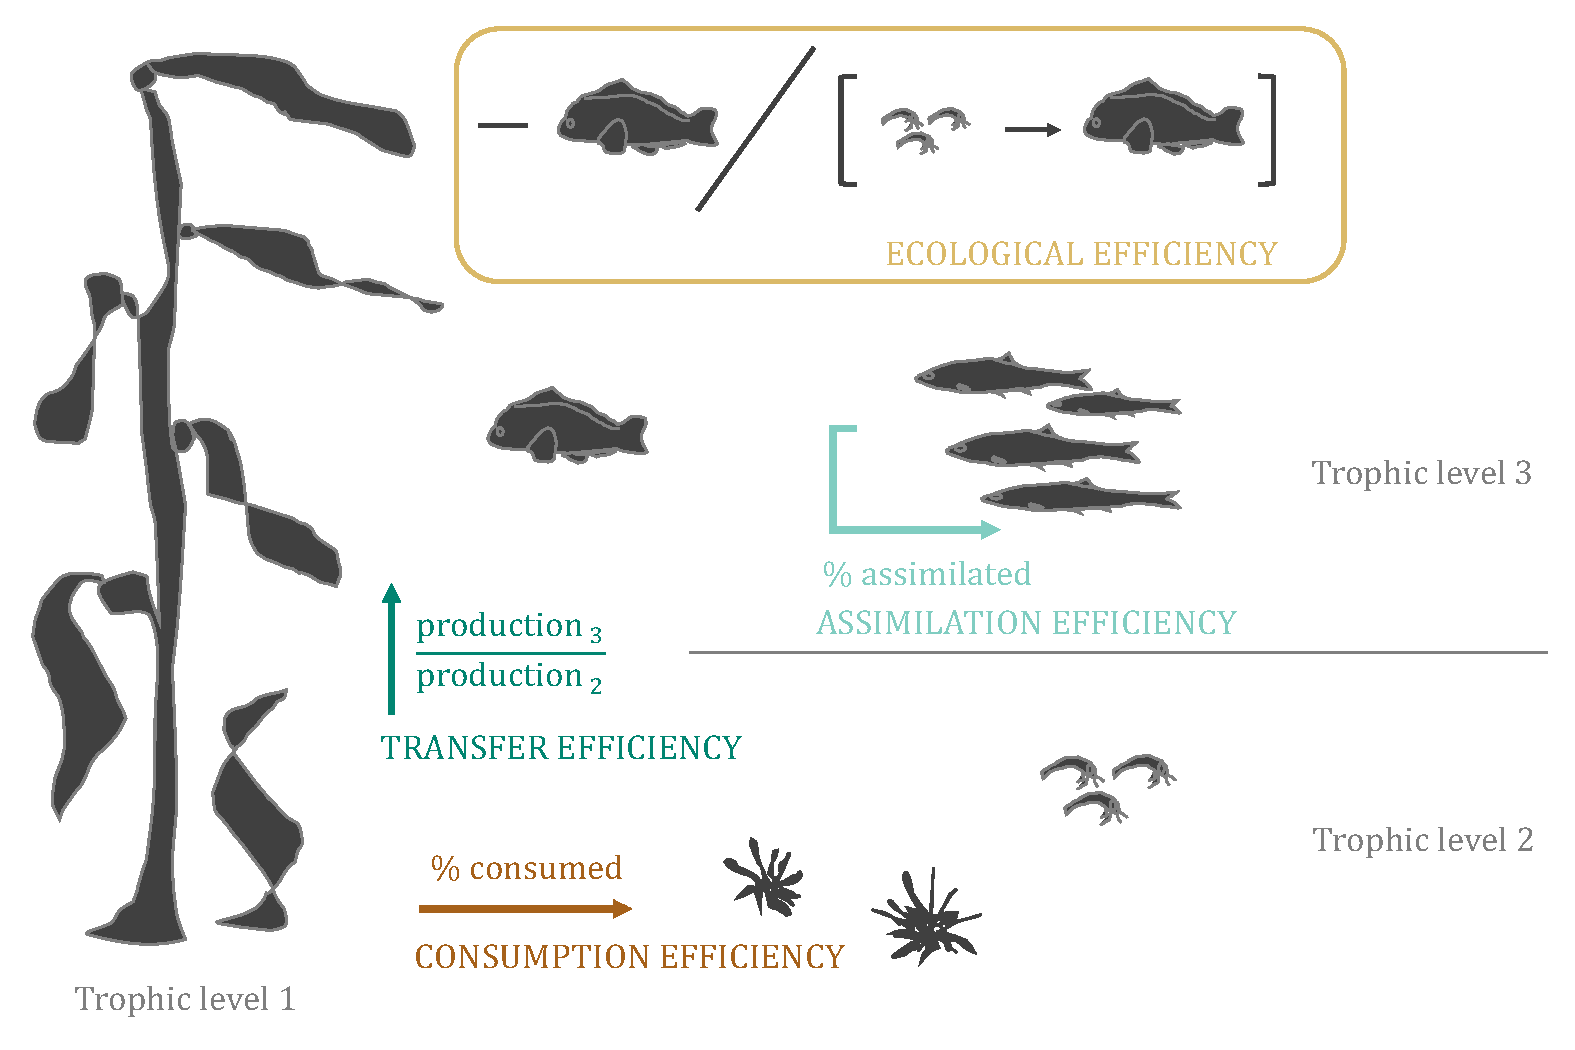
\includegraphics[width=\textwidth]{fig/foodwebimage}
    \caption{Cartoon of a food web that visualizes different efficiencies. The consumption efficiency is in brown, the transfer efficiency is in teal, the assimilation efficiency is in light blue, and the ecological efficiency (food chain efficiency) is in tan. In the consumption and ecological efficiency, the head of the arrow indicates the direction of consumption, where the species at the arrow head represent the species consuming the species at the arrow's origin. The diagram of the ecological efficiency includes a negative sign, division sign, and parentheses. Plot created using Microsoft office 2013.}
    \label{foodweb}
\end{figure}

The confusion around the definition is not the only complication with transfer efficiency--the values themselves have been disputed over the years and remain a point of contention. It is surprising that some scholars treat transfer efficiency as a fixed constant (i.e., 10\%) for all trophic levels in light of the fact that other scholars have found that physiological, and potentially behavioral, characteristics influence transfer efficiency \cite{may1983ecology, pauly1995primary, ware2000aquatic, cury2005trophodynamic, libralato2008novel, chassot2010global, trebilco2013ecosystem, watson2014primary}.

\subsection{Physiological and Behavioral Characteristics of Transfer Efficiency in Freshwater and Marine Ecosystems}
Multiple factors have been shown to affect transfer efficiency in both freshwater and marine ecosystems. In freshwater systems, the sources of variability in transfer efficiencies include the body of water, season, trophic level, and species composition \cite{lindeman1942trophic, gaedke1994seasonal, rybarczyk2003analysis, karlsson2007differences}.
In marine systems, transfer efficiency varies by ecological system, geographic location, trophic level, metabolic strategy, and species composition \cite{may1983ecology, persson2007food, libralato2008novel, barnes2010global}.

\subsubsection{Ecological System Within Freshwater and Marine Ecosystems}
Transfer efficiency has been found to be specific to the geographical region. Multiple marine studies found distinct transfer efficiencies between upwelling, temperate and tropical ecosystems (i.e., 5\% upwelling, 10\% temperate, and 14\% tropical) \cite{libralato2008novel, coll2008ecosystem, chassot2010global}. Even within a single ecosystem,
\citet{baird2004energy} found that each community within an intertidal ecosystem had unique transfer efficiency values. Distinct transfer efficiency values have also been found to occur not only between lakes and within trophic levels in freshwater ecosystems \cite{lindeman1942trophic}, but also in bays and estuaries as well \cite{rybarczyk2003analysis}.

\vspace{5mm}

Additionally, research has found that the amount of sunlight a region receives affects transfer efficiency. \citet{sanmartin2006latitudinal} suggest that transfer efficiency from phytoplankton to zooplankton in marine ecosystems decreases as latitude increases due to the decrease in sunlight. \citet{gaedke1994seasonal} found seasonal variation in transfer efficiency between the first and second trophic level in lakes, with transfer efficiency rising in the summer and fall and decreasing in the winter and spring. The seasonal variation in transfer efficiency can be attributed to the decrease in phytoplankton abundance in winter due to limited sunlight. As daylight increases in early spring, there is a gradual increase in phytoplankton blooms--culminating in the maximum phytoplankton production in summer (i.e., peak hours of sunlight).  As the days become shorter in fall and the hours of sunlight decreases, there is a decrease in the amount of phytoplankton. There is a time lag corresponding to the change in sunlight in the spring and fall seasons. Therefore, the amount of sunlight indirectly influences transfer efficiency between the first and second trophic level by directly impacting the phytoplankton abundance. 

\subsubsection{Trophic Level}
Size spectrum studies report that transfer efficiency decreases with body size, and by association, trophic level \cite{barnes2010global}. Therefore, the size ratio of prey to predators (e.g., phytoplankton to zooplankton) impacts transfer efficiency and trophic structure 
\cite{havens1998size, garciacomas2016prey}.

\subsubsection{Metabolic Strategy}
Furthermore, \citet{may1983ecology} found ectotherms are more efficient than endotherms in transferring energy from trophic level $n$ to trophic level $n+1$, with energy transfer efficiencies around 20-50\% for invertebrate ectotherms, around 10\% for vertebrate ectotherms and less than 2\% for endotherms. This discrepancy in transfer efficiency is due to the metabolic efficiency: ectotherms rely on environmental heat sources and therefore have a lower metabolic cost in comparison to endotherms. Much of the metabolic energy in endotherms goes to the production of heat. Therefore, transfer of energy in the higher trophic levels where endotherms are prominent is less than the lower trophic levels were ectotherms make up more of the composition in marine ecosystems \cite{mcgarvey2018two}.

\subsubsection{Species Composition}
Consuming nutritionally imbalanced food has been shown to lead to large respiratory losses, which negatively affect transfer efficiency \cite{persson2007food}. \citet{karlsson2007differences} and \citet{vonelert2003absence} found that the species composition of prey, in particular different species of zooplankton crustaceans and the absence of long-chain polyunsaturated fatty acid in cyanobacteria, influence transfer efficiency. In addition, the presence of jellyfish blooms has been found to reduce the transfer of energy to higher trophic levels \cite{condon2011jellyfish}.

\vspace{5mm}

\citet{trussell2006fear} and \citet{schmitz2008individuals} found that the risk of predation modifies prey conversion efficiencies and biomass production, which could therefore influence trophic structure and energy transfer. While these results refer specifically to assimilation and consumption efficiencies, it is plausible that this behavior influences transfer efficiencies as well. While the specific factors  previously discussed influence transfer efficiency individually, these components interact in the natural environment. Because of this interaction, researchers must consider the impacts of the synergistic effects of these factors on the variability of the transfer efficiency and in turn how to account for them in the modeling process.  

\subsection{The 10\% Transfer Efficiency}
Although the studies above highlight that a number of factors can greatly affect trophic efficiencies, we still see broad use of the assumption of a constant value of 10\%. To explore how (un)reasonable this assumption might be in different contexts, we synthesize the pattern of variation that has been observed in empirical studies that measured transfer efficiencies. Our goal is to provide guidance for what is reasonable to assume and what is necessary to measure.

\vspace{5mm}

It is unclear where the 10\% transfer efficiency assumption came from. Looking back at the historical records, we find a ``tangled web" of misattributions and a general lack of empirical evidence. \citet{semper1881animal} might have come up with the theory that there is a 10\% transfer between trophic levels, but he lacked empirical evidence to back this claim \cite{mcintosh1986background}. \citet{lindeman1942trophic} developed more general theory by looking at energy flow diagrams and mentioned a progressive efficiency which is currently known as transfer efficiency. However, no explicit mention of a 10\% value shows up in this work even though he is often credited for it (i.e., Lindeman?s law of trophic transfer efficiency--\citealt{chapman1998ecology}). \citet{slobodkin1959energetics, slobodkin1972inconstancy} stated that ?the values mentioned by Lindeman, as well as other values presented by other field workers, for ecological efficiency tended to cluster around 10\%.? Yet, Lindeman never explicitly discusses the ecological efficiency. He talked about the progressive efficiency, which as mentioned previously is a different concept. Regardless, Slobodkin and his students used laboratory experiments to formalize the hypothesis that there was an approximately 10\% transfer between trophic levels \cite{slobodkin1959energetics}. He referred to this as the food chain efficiency, which was later renamed to the ecological efficiency. However in a later study, \citet{slobodkin1972inconstancy} found empirical and theoretical objections to the 10\% ecological efficiency and rejected the theory. According to \citet{mcintosh1986background}, ?Nevertheless, May (1967b) in pursuit of the ?perfect crystals? of ecology, included Slobodkin?s 1961 hypothesis in a series of community properties he described as ?constant and predictable?.? In a more recent edition of May?s Theoretical Ecology textbook , however, the authors reach a very different conclusion:

\begin{quote}
One such [generalization] in the early 1960s suggested that the food-chain efficiency for transfer of energy from one trophic level to the next was generally around 10\%. Subsequent studies showed that such food-chain efficiencies can vary over two or more orders of magnitude, from less than 0.1\% to significantly more than 10\%. Some evidence suggests such efficiencies may, other things being equal, be higher for carnivores and detritus feeders than for herbivores, possibly because biochemical conversion efficiencies are higher for animals eating plants. \cite{may2007theoretical}
\end{quote}

In Figure \ref{flowchart}, we present a flowchart showing the muddled origin of this concept. Given the unclear origin and application of the 10\% transfer efficiency assumption, this assumption warrants further analysis, which is the focus of this current study. In the following section, we synthesize studies that provide empirical estimates of transfer efficiencies.

\begin{figure}[H]
     \centering
       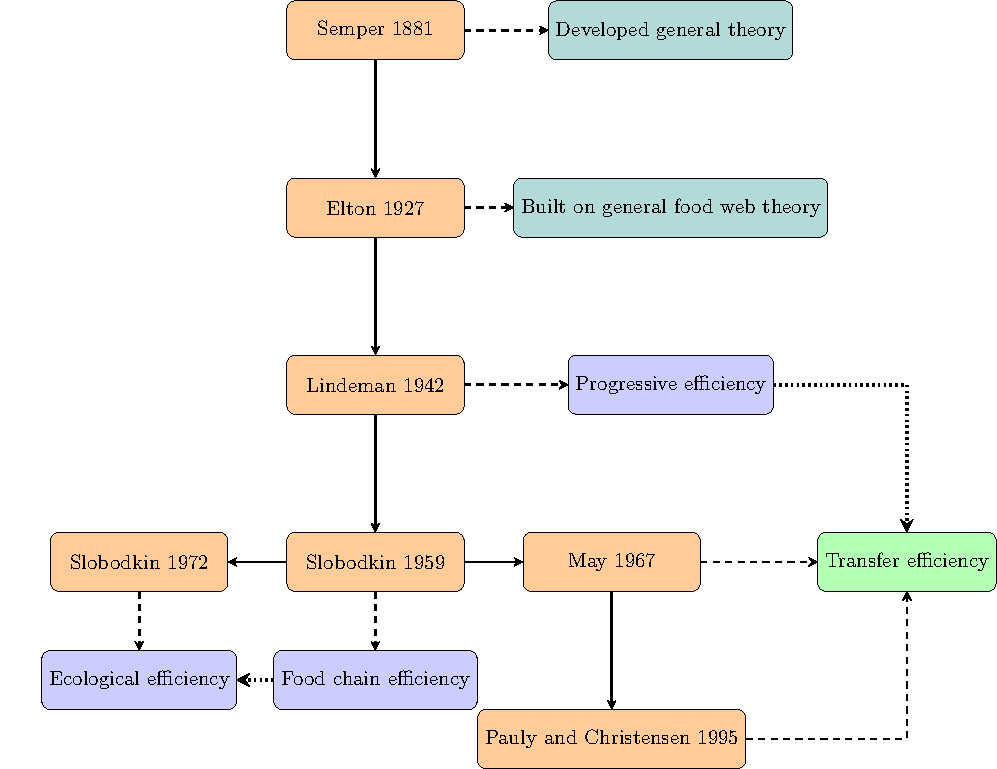
\includegraphics[width=\textwidth]{fig/flowchartfig}
    \caption{Flow chart of the origin of the 10\% transfer efficiency theory (green icon). A subset of key journal articles are highlighted in the orange icons. The dashed lines point to the efficiency mention in a particular article. The dotted lines represent a change in the name of an efficiency. Teal icons denote that the article discussed general theory, while periwinkle blue icons represent the discussion of a type of efficiency. The arrowhead attached to the solid line denotes the downstream flow direction of citations. Plot created using LaTeX v.2.9.6211  \cite{lamport1994latex} package tikz v.3.0.1a \cite{tantau2015tikz}.}
    \label{flowchart}
\end{figure}

\section{Methods}
To explore the empirical distributions of transfer efficiencies, we collected  articles that mentioned both food web and transfer efficiency. We then selected from these studies those that included relevant data, whether model-based or empirical. While we initially hoped to include terrestrial as well as freshwater and marine studies, we found nearly all of the terrestrial studies were on the consumption and assimilation efficiency, not the transfer efficiency. Therefore, we broke our analysis into two sections: freshwater and marine and ignored terrestrial. We primarily applied exploratory data analysis techniques such as summary statistics to distinguish patterns between the systems. 

\vspace{5mm}

If the sample size was sufficient large, we also used decision tree analysis (i.e., regression trees with pruning, bagging, and random forests) and Monte Carlo simulations (See Table \ref{datafresh} and \ref{datamar}). Decision tree analysis was employed to determine which factors had the largest impact on transfer efficiency. Using an approach similar to \cite{libralato2008novel}, we clustered the marine ecosystems into the following regions: temperate shelves and seas, tropical shelves and seas, lagoons, upwelling ecosystems, and open oceans. Although we also clustered the freshwater ecosystems into lakes, springs, and ponds, the sample size of the freshwater transfer efficiency data was too small to run regression tree analysis. We used regression trees with pruning, bagging, and random forests on the marine transfer efficiency data set and used relative importance plots to determine which factors accounted for the largest sources of variation and were most useful in predicting transfer efficiency. In the discussion, we used Monte Carlo simulations to aid in the conversation.

\subsection{Freshwater}
Many of the preliminary studies on transfer efficiency occurred in freshwater systems. All of the early studies were empirical (i.e., data used to calculate the transfer efficiency were collected either through laboratory experiments or from the field), but over time studies shifted to being increasingly model-based (i.e., data used to calculate the transfer efficiency were generated as the product of computer models). We found a total of 11 systems with transfer efficiency data (Table \ref{datafresh}). Only the empirical studies reported transfer efficiency values for multiple trophic levels. The model-based studies reported the system-wide average. Most of the transfer efficiency data is empirically based. 

\vspace{5mm}

The distributions of the freshwater transfer efficiencies are given in Figure \ref{dens_te}. The empirical observations are skewed-right, while the model-based observations appear bimodal (albeit with a small sample size--$n=4$). Combining the empirical and model-based estimates, the collective freshwater transfer efficiencies ($n=19$) range from 0.1\% to 22.3\% with a median of 8.4\%. When we calculate the average transfer (progressive) efficiency values provided in \citet{lindeman1942trophic}, we found that the average actually is 9\%. If we consider just transfer efficiencies between phytoplankton (trophic level 1) and zooplankton (trophic level 2), we found the median transfer efficiency to be 12.2\%. Unfortunately, the sample size in each group (i.e., trophic level and geographical region) is insufficiently large to draw any strong conclusions with relative certainty about which factors are the biggest sources of variation.

\begin{figure}[H]
     \centering
       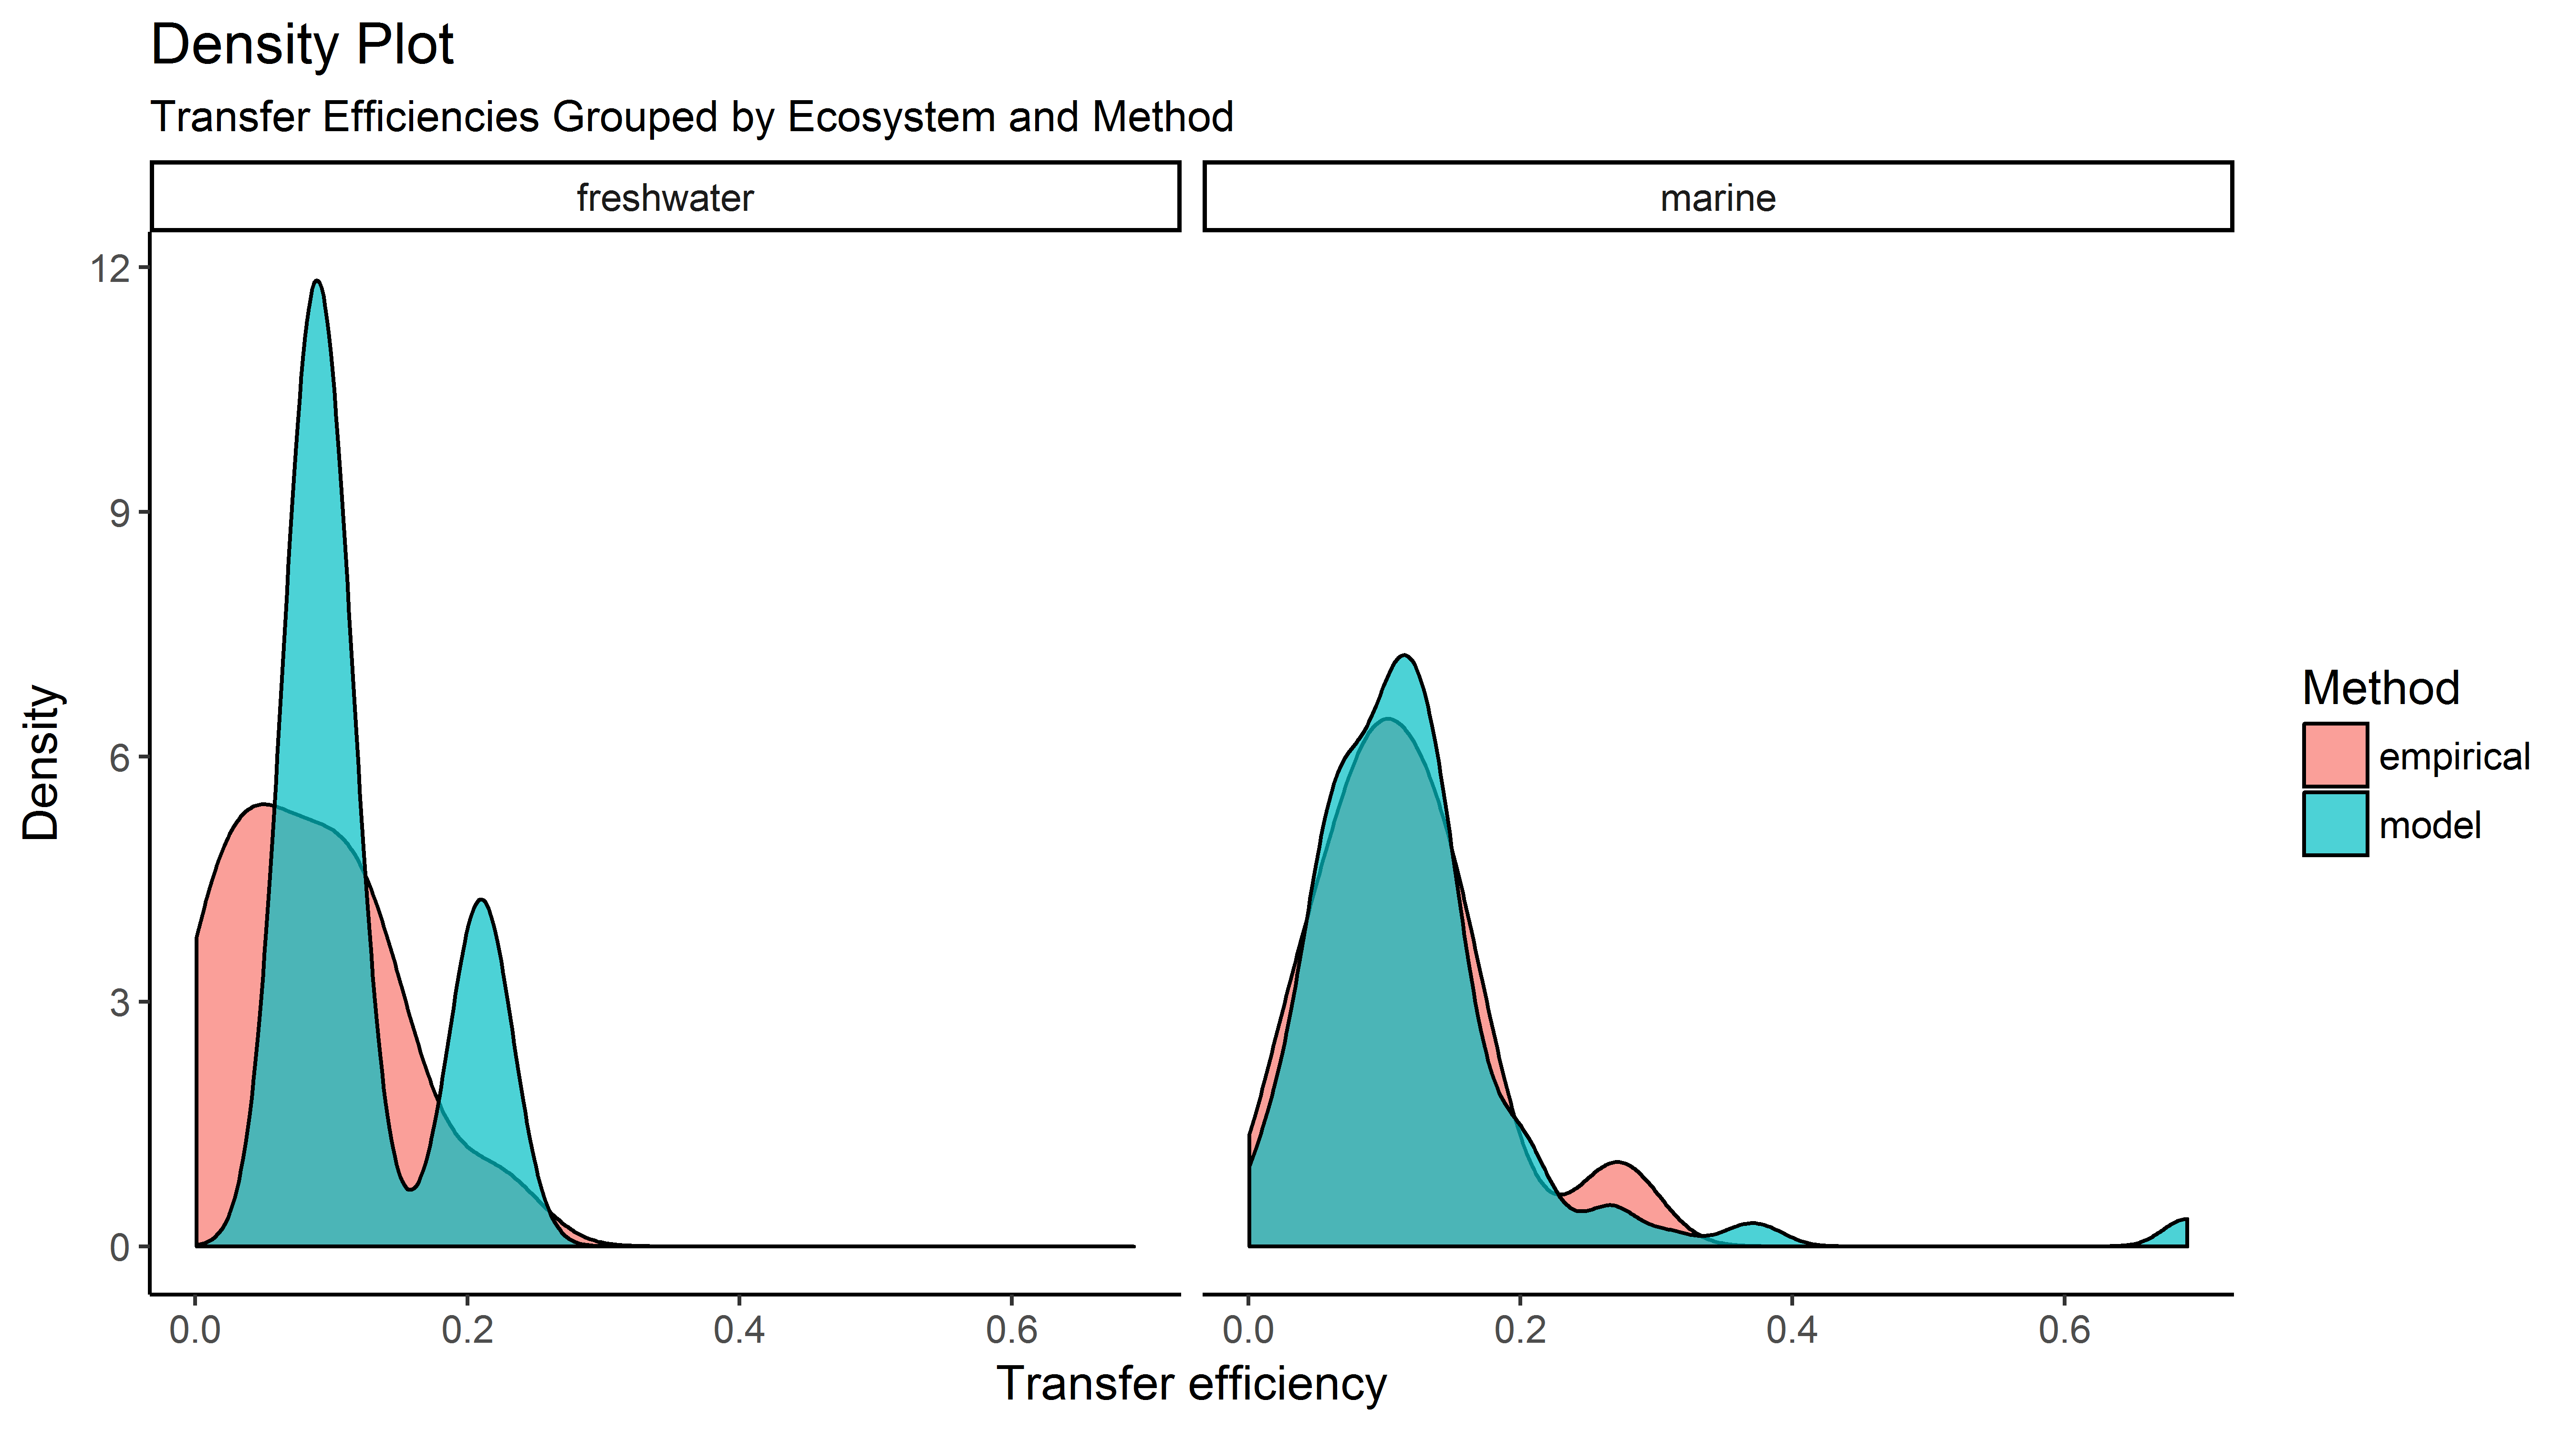
\includegraphics[width=\textwidth]{fig/density_eco_method}
    \caption{Density plot of transfer efficiencies where transfer efficiencies are grouped by ecosystem (i.e., freshwater vs. marine) and method (i.e., empirical and model-based).  There are a total of 15 transfer efficiency observations gathered from freshwater empirical studies, 4 observations from freshwater model-based studies, 13 from marine empirical studies, and 134 from marine model-based studies. Plot created using R v.3.4.3 \cite{Rcite} ggplot2 package v.2.2.1 \cite{ggplot}. }
    \label{dens_te}
\end{figure}

\small %starting font size 12, small means size 11pt
% Table generated by Excel2LaTeX from sheet 'Sheet1' with some big edits by Laura
%\begin{landscape}
\begin{longtable} {p{3cm}p{3cm}p{1.8cm}lp{2cm}p{1.7cm}} 
	\toprule
    Articles & Region & Clustered Region & Method & Trophic Level & Transfer Efficiency \\
    \midrule
    Chea et al. 2016   & Tonle Sap Great Lake & lakes & model & average & 8.3 \\
    Gaedke 1993   & Lake Constance & lakes & model & average & 21 \\
    Lindeman 1942   & Cedar Bog Lake & lakes & empirical & producers & 0.1 \\
    Lindeman 1942   & Cedar Bog Lake & lakes & empirical & primary consumers & 13.3 \\
    Lindeman 1942   & Cedar Bog Lake & lakes & empirical & secondary consumers & 22.3 \\
    Lindeman 1942   & Lake Mendota & lakes & empirical & producers & 0.4 \\
    Lindeman 1942   & Lake Mendota & lakes & empirical & primary consumers & 8.7 \\
    Lindeman 1942   & Lake Mendota & lakes & empirical & secondary consumers & 5.5 \\
    Lindeman 1942   & Lake Mendota & lakes & empirical & tertiary consumers & 13 \\
    Odum 1959   & Silver Springs & springs & empirical & producers & 1.2 \\
    Odum 1959   & Silver Springs & springs & empirical & primary consumers & 16 \\
    Odum 1959   & Silver Springs & springs & empirical & secondary consumers & 11 \\
    Odum 1959   & Silver Springs & springs & empirical & tertiary consumers & 5 \\
    Rand and Stewart 1998   & Lake Michigan & lakes & empirical & tertiary consumers & 3.2 \\
    Rand and Stewart 1998   & Lake Ontario & lakes & empirical & primary consumers & 11.1 \\
    Rand and Stewart 1998   & Lake Ontario & lakes & empirical & secondary consumers & 8.3 \\
    Rand and Stewart 1998   & Lake Ontario & lakes & empirical & tertiary consumers & 4.6 \\
    Villaneuva et al. 2008   & Lake Kivu & lakes & model & average & 8.4 \\
    Villaneuva et al. 2006   & Lake Nokoue & lakes & model & average & 10.3 \\
    \bottomrule
    \caption{Freshwater transfer efficiency data}
         \label{datafresh}
    \end{longtable}
% \end{landscape}
\normalsize

\subsection{Marine}
Marine studies on transfer efficiency did not commence until decades after the start of freshwater studies. The popularity of marine transfer efficiency research has increased rapidly in the past 20 years and has overall now exceeded the number of freshwater studies. A total of 115 sites have transfer efficiency data (Table \ref{datamar}). In contrast to the freshwater studies, most marine transfer efficiency data ($n=134$) come from model-based studies rather than empirical experiments ($n=13$). Most marine studies report the average value for an entire system ($n=94$). In studies that focused on individual transfer efficiencies between specific trophic levels, most focused on the transfer efficiency between phytoplankton (trophic level 1) and zooplankton (trophic level 2).

\vspace{5mm}

The empirical and model-based transfer efficiency data both form skewed-right distributions with large amounts of dispersion around the 10\% value (Figure \ref{dens_te}). For model-based observations, there are a few outlying points from a study on bays and estuaries that skew the distribution (Figure \ref{dens_te}). The combined transfer efficiency data ranges from 0.2\% to 69\% with a median of 10.6\%, while the range constricts with a minimum of 3.12\% to a maximum of 27.2\% for just the marine empirical studies (Figure \ref{dens_te}). 

\vspace{5mm}

To explore the potential drivers of variation in transfer efficiencies, we calculated importance plots from the decision tree analysis. When interpreting importance plots, the larger the score, the more influential the variable. A number close to zero indicates the variables is not important and could be dropped. When determining the importance of a variable, the mean decrease in accuracy (i.e., mean square error, MSE) or the mean decrease in node impurity are used to measure how well the trees split the data. Thus, the relative importance plots from the decision tree analysis indicate that trophic level had the greatest influence on transfer efficiency, followed by the clustered region (i.e., temperate shelves and seas, tropical shelves and seas, lagoons, upwelling ecosystems, and open oceans) (Figure \ref{varimp}). The method employed (i.e., empirical or model-based) did not appear to be a useful predictor.  

\begin{figure}[H]
     \centering
       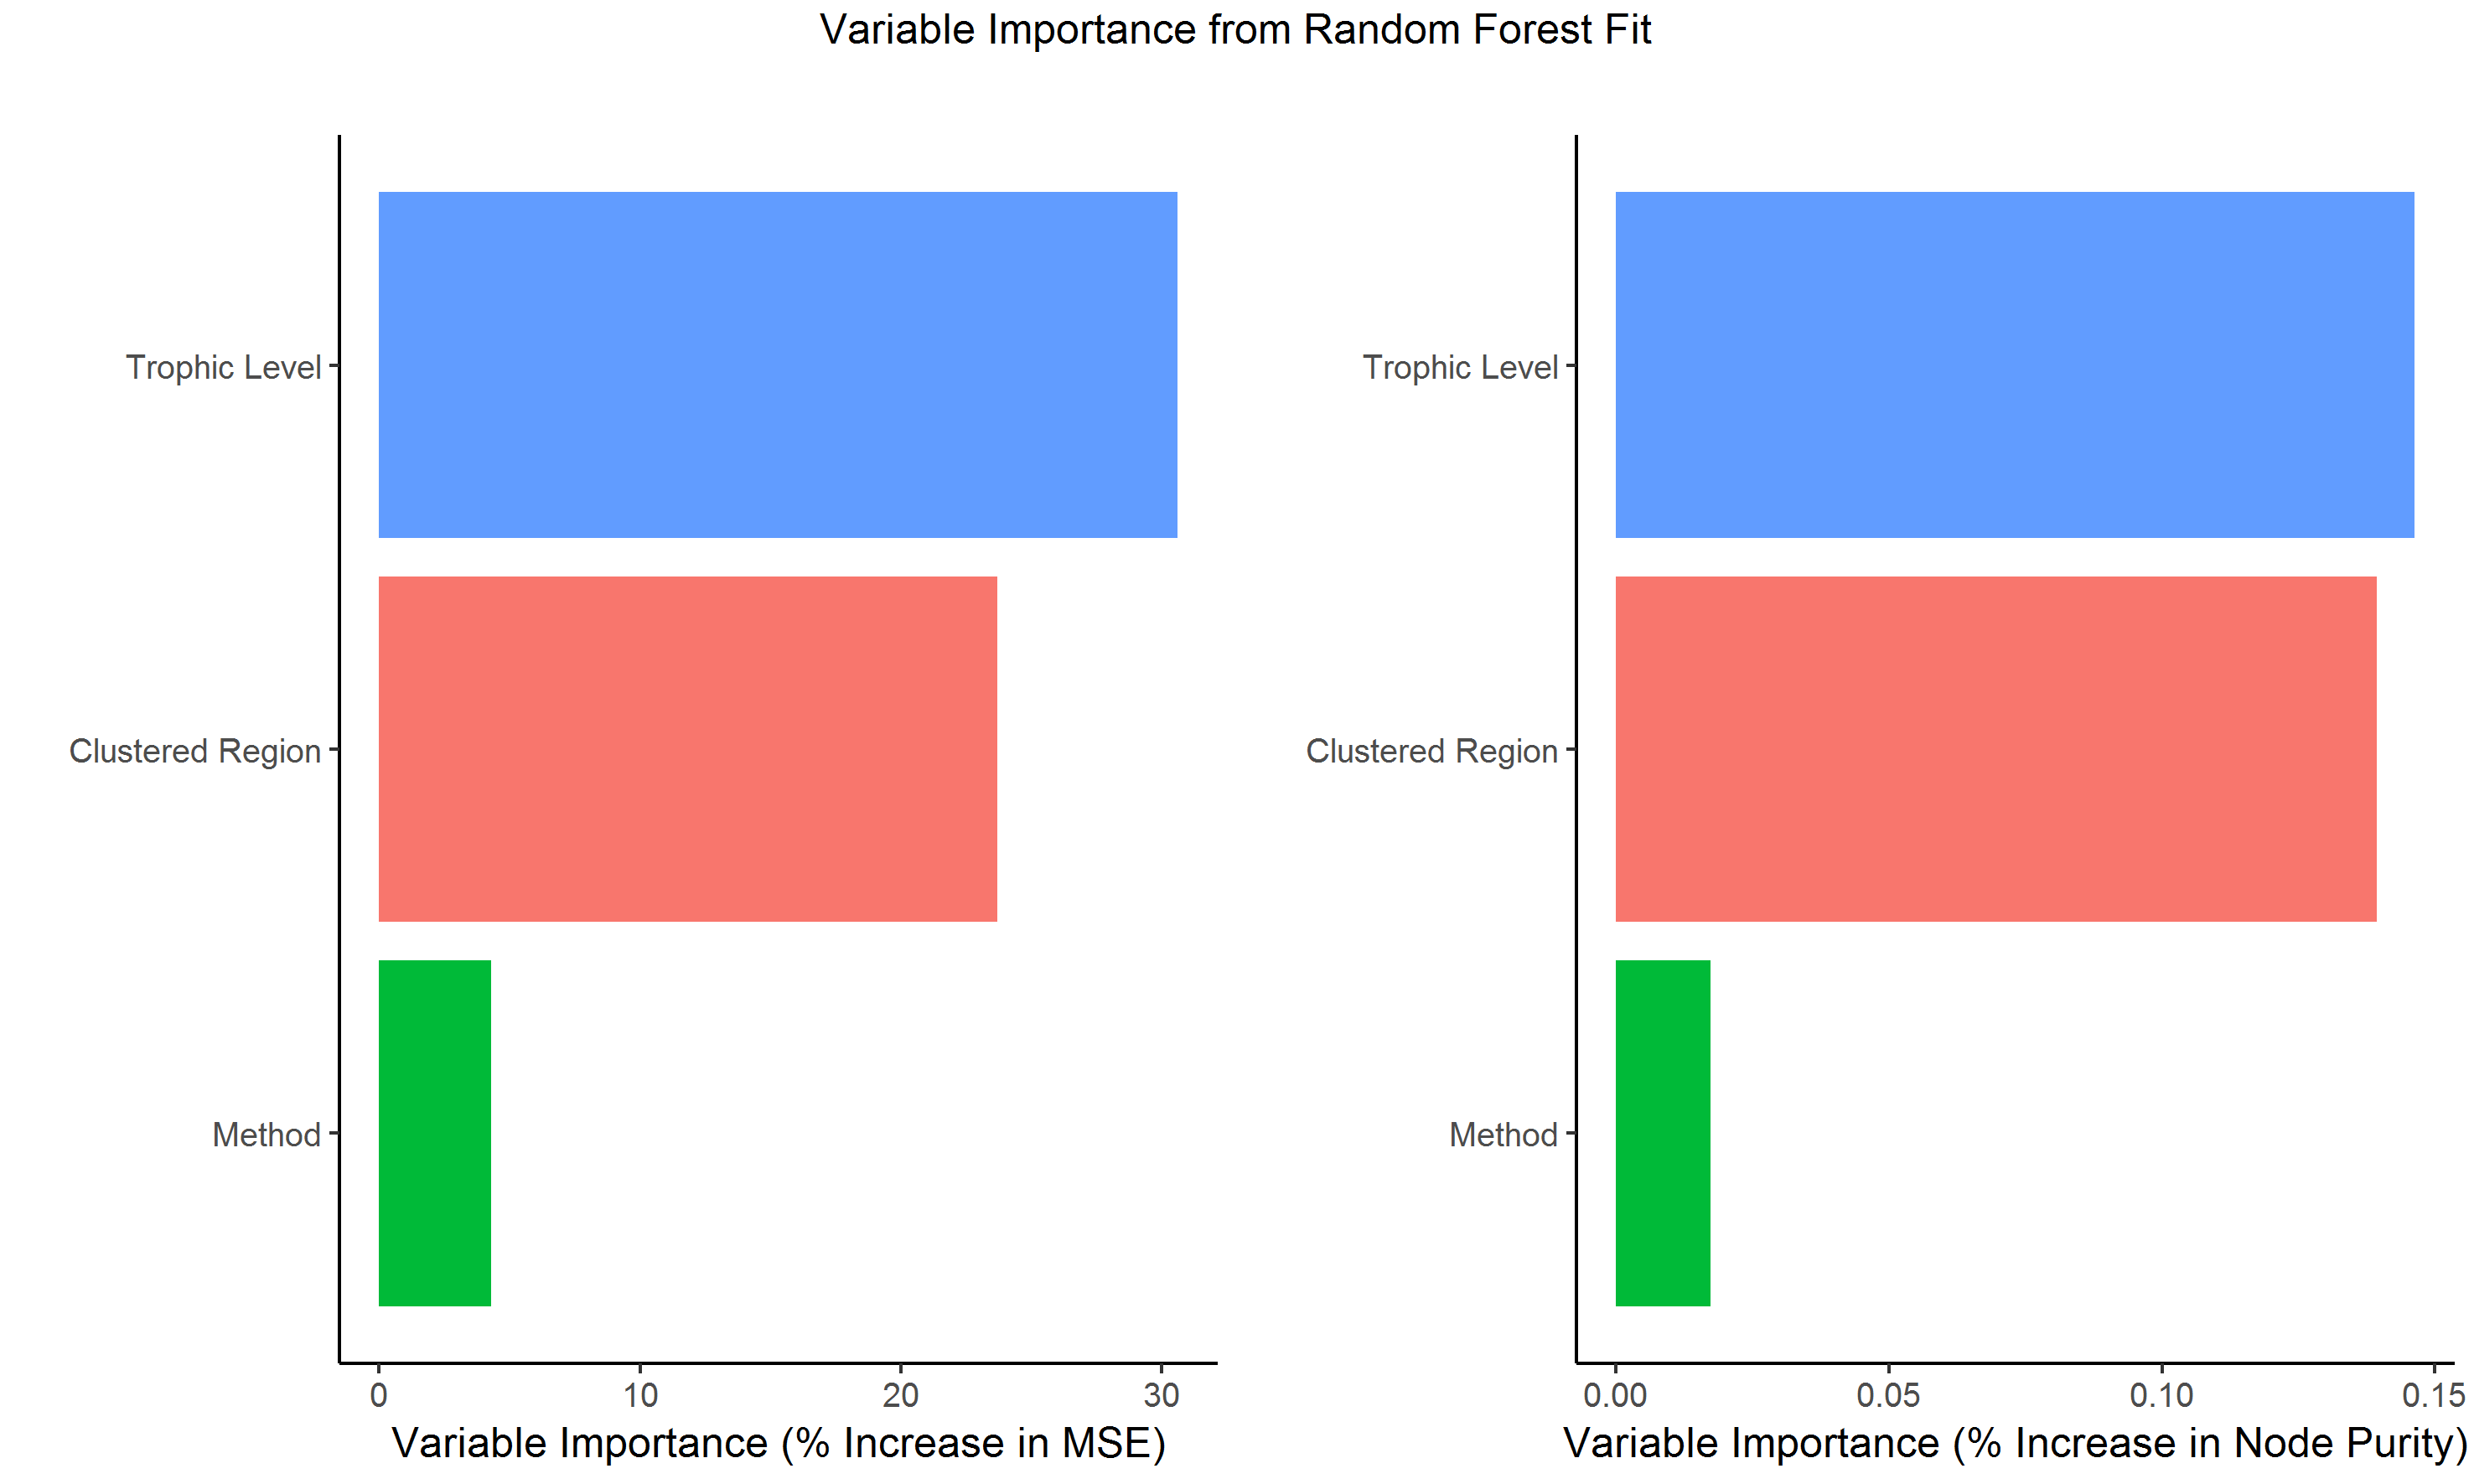
\includegraphics[width=\textwidth]{fig/var_imp_plot}
    \caption{Relative importance plots for random forest fit on marine transfer efficiency observations. In panel a), the predictors are ordered by percent increase in Mean Square Error (MSE). In panel b), the predictors are ordered by increase in node purity. Plot created using R v.3.4.3 \cite{Rcite} ggplot2 package v.2.2.1 \cite{ggplot}. }
    \label{varimp}
\end{figure}

We combined results across both marine and freshwater systems to examine differences among trophic levels (Figure 5). We combined data for all the systems to increase the sample size. Whether the different densities are due to the sensitivity to small samples sizes or systematic differences is unclear. Nonetheless, our results support the hypothesis that transfer efficiency decreases as trophic level increases (see \citealt{garcia2012reconsidering}). This in turn supports the results from  \citet{may1983ecology} that in the marine environment ectotherms (invertebrates then vertebrates), which dominate the lower trophic levels, are more efficient than endotherms, which are more prominent at higher trophic levels (Figure \ref{den_tl}). 

\begin{figure}[H]
     \centering
       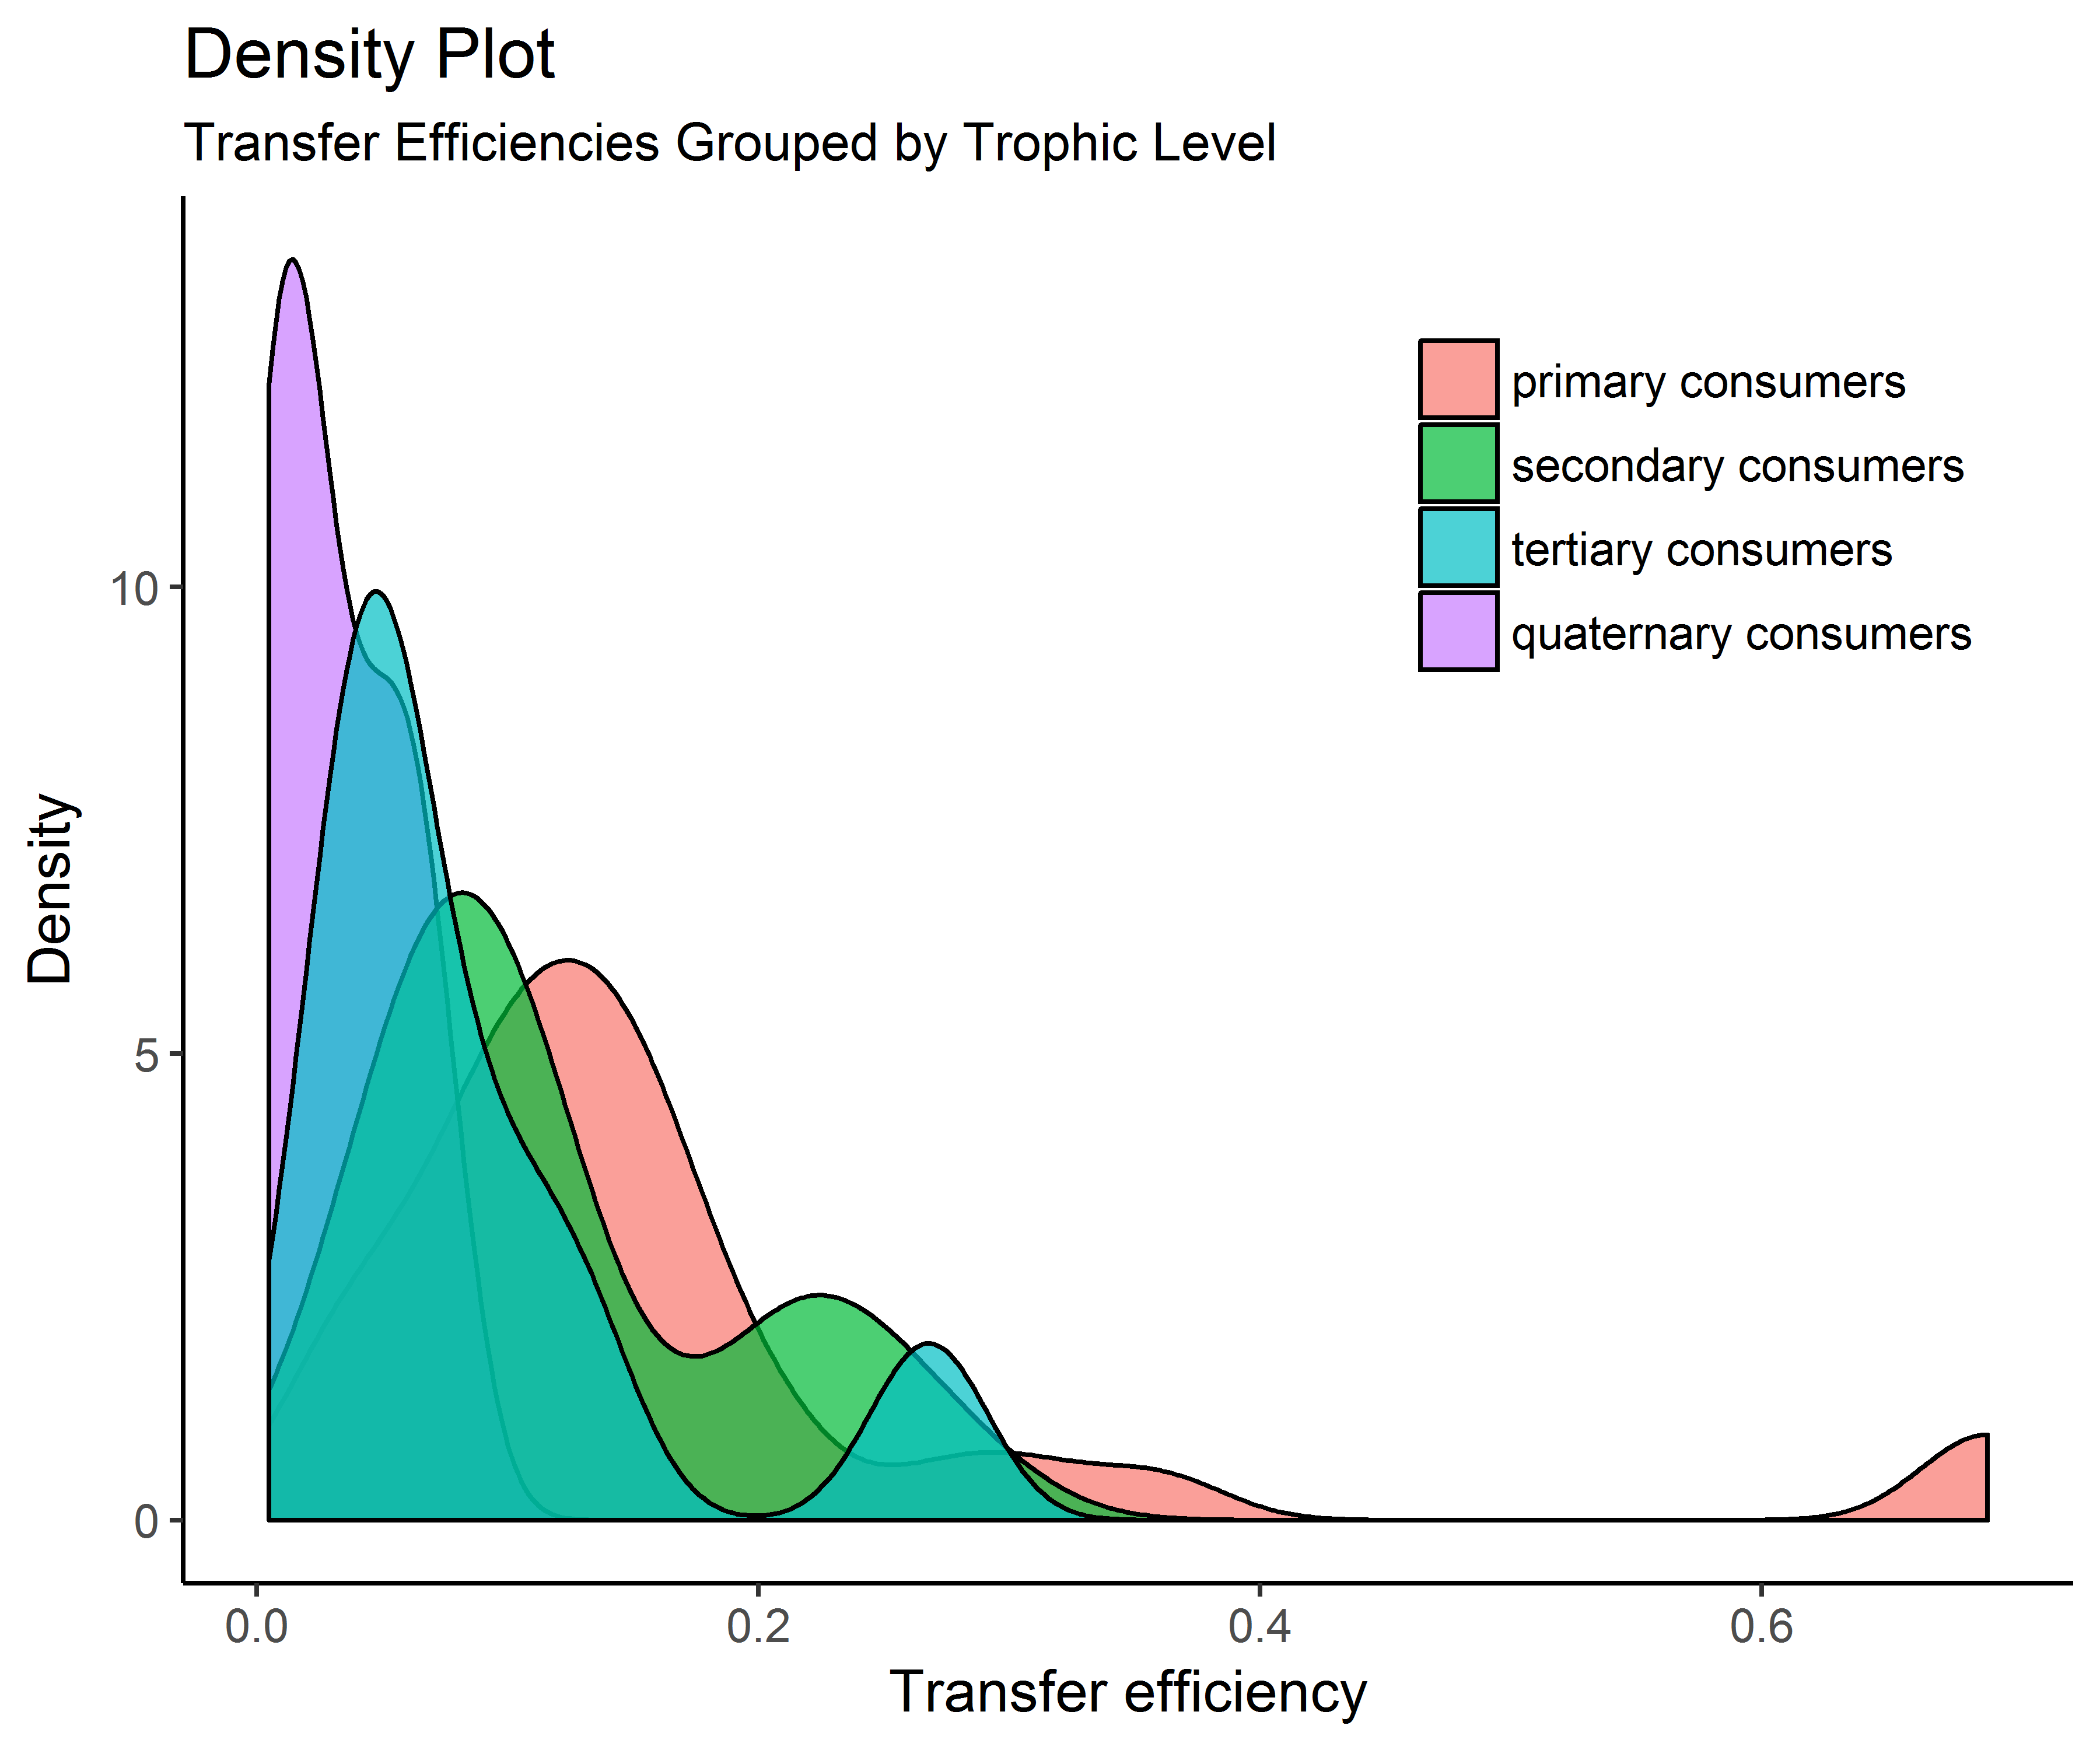
\includegraphics[width=.8\textwidth]{fig/density_te_by_tl}
    \caption{Density plot of transfer efficiencies grouped by trophic level. The data in this figure includes both ecosystem (i.e., freshwater and marine) and empirical and model-based transfer efficiency data. Plot created using R v.3.4.3 \cite{Rcite} ggplot2 package v.2.2.1 \cite{ggplot}. }
    \label{den_tl}
\end{figure}

\small %starting font size 12, small means size 11pt
% Table generated by Excel2LaTeX from sheet 'Sheet1' with some big edits by Laura
%\begin{landscape}
\begin{longtable} {p{3cm}p{3cm}p{1.8cm}lp{2cm}p{1.7cm}}
	\toprule
    Articles & Region & Clustered Region & Method & Trophic Level & Transfer Efficiency \\
    \midrule
    \endhead
    Akoglu et al. 2014  & Black Sea & temperate seas & model & primary consumers & 3 \\
    Akoglu et al. 2014   & Black Sea & temperate seas & model & secondary consumers & 3.8 \\
    Akoglu et al. 2014  & Black Sea & temperate seas & model & tertiary consumers & 7.4 \\
    Akoglu et al. 2014  & Black Sea & temperate seas & model & quaternary consumers & 0.5 \\
    Anjusha et al. 2013   & Gulf of Mannar & tropical seas & empirical & primary consumers & 13 \\
    Anjusha et al. 2013   & Gulf of Mannar & tropical seas & empirical & primary consumers & 12 \\
    Anjusha et al. 2013   & Gulf of Mannar & tropical seas & empirical & primary consumers & 14.6 \\
    Anjusha et al. 2013  & Gulf of Mannar & tropical seas & empirical & primary consumers & 9.1 \\
    Anjusha et al. 2013   & Gulf of Mannar & tropical seas & empirical & primary consumers & 6.8 \\
    Anjusha et al. 2013 & Palk Bay & tropical seas & empirical & primary consumers & 27.2 \\
    Anjusha et al. 2013   & Palk Bay & tropical seas & empirical & primary consumers & 17.6 \\
    Anjusha et al. 2013  & Palk Bay & tropical seas & empirical & primary consumers & 9.39 \\
    Anjusha et al. 2013  & Palk Bay & tropical seas & empirical & primary consumers & 7.19 \\
    Anjusha et al. 2013  & Palk Bay & tropical seas & empirical & primary consumers & 3.12 \\
    Anjusha et al. 2013  & Palk Bay & tropical seas & empirical & primary consumers & 3.23 \\
    Baird et al. 2004  & Sylt-Romo Bight & temperate seas & model & average & 2.61 \\
    Baird et al. 2007  & Sylt-Romo Bight: arenicola flats & temperate seas & model & average & 3.47 \\
    Baird et al. 2007  & Sylt-Romo Bight: dense zostera noltii beds & temperate seas & model & average & 5.58 \\
    Baird et al. 2007  & Sylt-Romo Bight: mud flats & temperate seas & model & average & 6.13 \\
    Baird et al. 2007   & Sylt-Romo Bight: muddy sand flats & temperate seas & model & average & 7.31 \\
    Baird et al. 2007   & Sylt-Romo Bight: mussel beds & temperate seas & model & average & 14.92 \\
    Baird et al. 2007  & Sylt-Romo Bight: pelagic domain & temperate seas & model & average & 1 \\
    Baird et al. 2007  & Sylt-Romo Bight: sandy beaches & temperate seas & model & average & 6.5 \\
    Baird et al. 2007  & Sylt-Romo Bight: sandy shoals & temperate seas & model & average & 3.3 \\
    Baird et al. 2007   & Sylt-Romo Bight: sparse zostera noltii beds & temperate seas & model & average & 5.06 \\
    Barnes et al.  2010  & summary of 21 locations & -    & model & average small sizes & 13.8 \\
    Barnes et al.  2010   & summary of 21 locations & -    & model & average large sizes & 5.8 \\
    Baumann 1995   & general claim & -    & empirical & average & 15 \\
    Bradford-Grieve et al. 2003   & Southern Plateau, New Zealand & temperate seas & model & secondary consumers & 23 \\
    Chassot et al. 2010  & temperate & temperate seas & model & average & 10 \\
    Chassot et al. 2010   & tropical & tropical seas & model & average & 14 \\
    Chassot et al. 2010  & upwelling & upwelling ecosystems & model & average & 5 \\
    Cornejo-Donoso and Antezana 2008   & Antarctic Peninsula & temperate seas & model & primary consumers & 21 \\
    Cornejo-Donoso and Antezana 2008  & Antarctic Peninsula & temperate seas & model & secondary consumers & 20 \\
    Cornejo-Donoso and Antezana 2008  & Antarctic Peninsula & temperate seas & model & tertiary consumers & 10 \\
    Cornejo-Donoso and Antezana 2008   & Antarctic Peninsula & temperate seas & model & quaternary consumers & 5 \\
    D'Alelio et al. 2016   & Gulf of Naples & temperate seas & model & primary consumers & 20 \\
    Duan et al. 2009  & Pearl River Estuary & tropical seas & model & average & 10.2 \\
    Gamito and Erzini 2004  & Ria Formosa lagoon, south Portugal & lagoons & model & primary consumers & 4.8 \\
    Gamito and Erzini 2004   & Ria Formosa lagoon, south Portugal & lagoons & model & secondary consumers & 6 \\
    Gamito and Erzini 2004   & Ria Formosa lagoon, south Portugal & lagoons & model & tertiary consumers & 3.5 \\
    Gamito and Erzini 2004   & Ria Formosa lagoon, south Portugal & lagoons & model & quaternary consumers & 1.2 \\
    Gamito and Erzini 2004   & Ria Formosa lagoon, south Portugal & lagoons & model & quinary consumers & 0.2 \\
    Libralto et al. 2008   & Atlantic coast of Morocco  & temperate seas & model & average & 10.9 \\
    Libralto et al. 2008   & Azores archipelago & temperate seas & model & average & 10.5 \\
    Libralto et al. 2008   & Bali Strait & tropical seas & model & average & 11.7 \\
    Libralto et al. 2008   & Baltic sea & temperate seas & model & average & 25.9 \\
    Libralto et al. 2008  & Bay of Bengal & tropical seas & model & average & 9 \\
    Libralto et al. 2008   & Bay of Biscay & temperate seas & model & average & 16.5 \\
    Libralto et al. 2008   & Bay of Revellata, Corsica & temperate seas & model & average & 18.8 \\
    Libralto et al. 2008   & Bolinao reef flat & tropical seas & model & average & 10.4 \\
    Libralto et al. 2008   & Brunei Darussalam & tropical seas & model & average & 12.9 \\
    Libralto et al. 2008  & California upwelling & upwelling ecosystems & model & average & 4 \\
    Libralto et al. 2008  & Campeche Bank of Yucatan shelf & tropical seas & model & average & 17.6 \\
    Libralto et al. 2008   & Cantabric Sea & temperate seas & model & average & 38.1 \\
    Libralto et al. 2008  & Celestun lagoon, Mexico & lagoons & model & average & 6.4 \\
    Libralto et al. 2008   & Central North Pacific Ocean & temperate seas & model & average & 4.4 \\
    Libralto et al. 2008   & Chesapeake Bay & temperate seas & model & average & 12.5 \\
    Libralto et al. 2008  & Chiku lagoon, Taiwan & lagoons & model & average & 13.1 \\
    Libralto et al. 2008  & Coast of Western Gulf of Mexico & tropical seas & model & average & 16.2 \\
    Libralto et al. 2008  & Coastal areas and reefs & -    & model & average & 13 \\
    Libralto et al. 2008  & Continental shelf of southern Brazil & tropical seas & model & average & 11.8 \\
    Libralto et al. 2008   & Eastern Bering Sea & temperate seas & model & average & 13.2 \\
    Libralto et al. 2008   & Eastern Scotian shelf & temperate seas & model & average & 11 \\
    Libralto et al. 2008   & Eastern Tropical Pacific Ocean & temperate seas & model & average & 20.4 \\
    Libralto et al. 2008  & Etang de Thau, France  & lagoons & model & average & 10.8 \\
    Libralto et al. 2008   & Faroe Islands & temperate seas & model & average & 14.4 \\
    Libralto et al. 2008  & Faroe Islands & temperate seas & model & average & 15.4 \\
    Libralto et al. 2008  & Floreana rocky reef Galapagos & tropical seas & model & average & 13 \\
    Libralto et al. 2008  &  Georgia Strait & temperate seas & model & average & 9.5 \\
    Libralto et al. 2008   & Great Barrier Reef & tropical seas & model & average & 11.5 \\
    Libralto et al. 2008  & Gulf of Lingayen & tropical seas & model & average & 13.5 \\
    Libralto et al. 2008   & Gulf of Maine - Georges Bank & temperate seas & model & average & 15.6 \\
    Libralto et al. 2008   & Gulf of Mexico continental shelf  & tropical seas & model & average & 9.7 \\
    Libralto et al. 2008  & Gulf of Thailand & tropical seas & model & average & 10.4 \\
    Libralto et al. 2008  & Hong Kong & tropical seas & model & average & 9.1 \\
    Libralto et al. 2008   & Icelandic fisheries & temperate seas & model & average & 14.2 \\
    Libralto et al. 2008   & Kuala Trengganu & tropical seas & model & average & 17.8 \\
    Libralto et al. 2008   & Laguna de Bay, Philippines & lagoons & model & average & 12.4 \\
    Libralto et al. 2008  & Lancaster Sound Region & temperate seas & model & average & 8.2 \\
    Libralto et al. 2008   & Maputo Bay & temperate seas & model & average & 7.6 \\
    Libralto et al. 2008   & Newfoundland & temperate seas & model & average & 14.3 \\
    Libralto et al. 2008  &  North Benguela upwelling & upwelling ecosystems & model & average & 7.9 \\
    Libralto et al. 2008 & North Coast of Central Java & tropical seas & model & average & 11.8 \\
    Libralto et al. 2008   & North Sea & temperate seas & model & average & 11.6 \\
    Libralto et al. 2008  & Northern British Columbia & temperate seas & model & average & 14.2 \\
    Libralto et al. 2008   & Northern Gulf of Saint Lawrence  & temperate seas & model & average & 12 \\
    Libralto et al.  2008   & Northern-central Adriatic Sea  & temperate seas & model & average & 10 \\
    Libralto et al. 2008  & Norwegian and Barents Sea & temperate seas & model & average & 10.5 \\
    Libralto et al. 2008  & NW Africa upwelling & upwelling ecosystems & model & average & 6.1 \\
    Libralto et al. 2008  & Open oceans & open oceans & model & average & 12 \\
    Libralto et al. 2008   & Orbetello lagoon & lagoons & model & average & 9.6 \\
    Libralto et al. 2008   & Peru upwelling & upwelling ecosystems & model & average & 6.6 \\
    Libralto et al. 2008   & Prince William Sound, Alaska & temperate seas & model & average & 14.1 \\
    Libralto et al. 2008  & San Miguel Bay & tropical seas & model & average & 20.6 \\
    Libralto et al. 2008  & San Pedro Bay & tropical seas & model & average & 9.4 \\
    Libralto et al. 2008   & Schlei Fjord & temperate seas & model & average & 7.4 \\
    Libralto et al. 2008   & Shallow areas of Gulf of Thailand & tropical seas & model & average & 6.8 \\
    Libralto et al. 2008   & South Catalan Sea & temperate seas & model & average & 12.6 \\
    Libralto et al. 2008   & South China Deep Sea & tropical seas & model & average & 10.6 \\
    Libralto et al. 2008   & Southern Brazil & tropical seas & model & average & 6.3 \\
    Libralto et al. 2008   & Southwest coast of India & tropical seas & model & average & 14 \\
    Libralto et al. 2008  & Tampa Bay & tropical seas & model & average & 8.6 \\
    Libralto et al. 2008  & Temperate shelves & temperate seas & model & average & 14 \\
    Libralto et al. 2008   & Tropical shelves & tropical seas & model & average & 10 \\
    Libralto et al. 2008   & Upwellings & upwelling ecosystems & model & average & 5 \\
    Libralto et al. 2008   & Venezuela northeastern shelf & tropical seas & model & average & 7.3 \\
    Libralto et al. 2008   & Venice lagoon & lagoons & model & average & 14.5 \\
    Libralto et al. 2008   & Vietnam-China shelf & tropical seas & model & average & 7.5 \\
    Libralto et al. 2008   & West Coast of Vancouver Island & temperate seas & model & average & 13.7 \\
    Libralto et al. 2008   & West Greenland  coast & temperate seas & model & average & 12.1 \\
    Libralto et al. 2008   & West Greenland trawling area & temperate seas & model & average & 7.1 \\
    Lin et al. 2006  &  Tapong Bay, southwestern Taiwan & tropical seas & model & average & 5.5 \\
    Liu et al. 2009  &  Nanwan Bay, southern Taiwan & tropical seas & model & primary consumers & 13.9 \\
    Liu et al. 2009  &  Nanwan Bay, southern Taiwan & tropical seas & model & secondary consumers & 6.6 \\
    Liu et al. 2009  & Nanwan Bay, southern Taiwan & tropical seas & model & tertiary consumers & 5.2 \\
    Liu et al. 2009   & Nanwan Bay, southern Taiwan & tropical seas & model & quaternary consumers & 2 \\
    Manickchand-Heileman et al. 2003   & Gulf of Paria, Venezuela and Trinidad & tropical seas & model & average & 12.2 \\
    Neira and Arancibia 2004   & upwelling Central Chile & upwelling ecosystems & model & primary consumers & 8.1 \\
    Neira and Arancibia 2004  & upwelling Central Chile & upwelling ecosystems & model & secondary consumers & 27.4 \\
    Neira and Arancibia 2004   & upwelling Central Chile & upwelling ecosystems & model & tertiary consumers & 26.8 \\
    Neira and Arancibia 2004   & upwelling Central Chile & upwelling ecosystems & model & quaternary consumers & 6.7 \\
    Neira and Arancibia 2004   & upwelling Central Chile & upwelling ecosystems & model & quinary consumers & 7.4 \\
    Pauly and Christensen 1995   & general claim & NA    & empirical & average & 10.13 \\
    Rybarczyk and Elkaim 2003   & Bay of Somme & temperate seas & model & primary consumers & 15.6 \\
    Rybarczyk and Elkaim 2003   & Chesapeake Bay & temperate seas & model & primary consumers & 31 \\
    Rybarczyk and Elkaim 2003  & Delaware Bay & temperate seas & model & primary consumers & 69 \\
    Rybarczyk and Elkaim 2003   & Narragansett Bay & temperate seas & model & primary consumers & 69 \\
    Rybarczyk and Elkaim 2003   & Seine Estuary & temperate seas & model & primary consumers & 36.05 \\
    Sheldon et al. 1977  &  ocean pelagic & open oceans & model & primary consumers & 15 \\
    Tsagarakis et al. 2010  & N. Aegean & temperate seas & model & average & 17.4 \\
    Tsagarakis et al. 2010  & N.C. Adriatic  & temperate seas & model & average & 10 \\
    Tsagarakis et al. 2010   & S. Catalan & temperate seas & model & average & 12.6 \\
    Villaneuva et al. 2006  & Ebrie lagoon  & lagoons & model & average & 15.5 \\
    Ware 2000  & Georges Bank & temperate seas & model & primary consumers & 15.9 \\
    Ware 2000   & Gulf of Maine & temperate seas & model & primary consumers & 11.9 \\
    Ware 2000  & Gulf of Maine & temperate seas & model & secondary consumers & 10.5 \\
    Ware 2000  & Mid-Atlantic Shelf & tropical seas & model & primary consumers & 10.2 \\
    Ware 2000   & Mid-Atlantic Shelf & tropical seas & model & secondary consumers & 10.1 \\
    Ware 2000   & Nova Scotia Shelf & temperate seas & model & primary consumers & 12.1 \\
    Ware 2000   & Nova Scotia Shelf & temperate seas & model & secondary consumers & 12.3 \\
    Ware 2000   & Oyashio current model & temperate seas & model & primary consumers & 17 \\
    Ware 2000   & Oyashio current model & temperate seas & model & secondary consumers & 7.9 \\
    Ware 2000   & SW Britisth Columbia model & temperate seas & model & primary consumers & 11.1 \\
    Ware 2000   & SW Britisth Columbia model & temperate seas & model & secondary consumers & 8 \\
    \bottomrule
    \caption{Marine transfer efficiency data}
    \label{datamar}
    \end{longtable}
% \end{landscape}
\normalsize


\section{Discussion}
Overall, these studies show similarities between the two systems. The results give visual evidence that although the average transfer efficiency does not differ greatly from 10\%, there is substantial variation in transfer efficiency in both systems (Figure \ref{dens_te}). Additionally our study was able to identify that trophic level and the general geographic location of the ecosystem impacts the variability of the transfer efficiency. Some of this large variation seems to have predictable patterns, but the potential sources of this variation can only be explored for the larger sample sizes from marine systems. Thus in the absence of data, the distributions generated in the current study are good starting points to model the variation in transfer efficiency. 

\vspace{5mm}

We hypothesize the difference in transfer efficiency between trophic levels could be partially attributed to the composition of the taxa. Additionally, the differences could be due to the mobility of the organisms at each trophic levels and the amount of energy expedited to capture their prey. Both of these points highlight the need for additional research that can distinguish between the different mechanisms that influence transfer efficiency (e.g., endotherms vs. ectotherms).

\vspace{5mm}

We encountered two main difficulties in this study due to the different naming conventions in the early states (Figure \ref{foodweb} and \ref{flowchart}) and the different efficiencies of interest amongst different fields. We bring this point up to highlight the challenges in conducting interdisciplinary work. We found freshwater studies report either assimilation and consumption efficiencies or transfer efficiency, while the majority of marine papers focused on transfer efficiency. As previously mentioned, we found very few terrestrial studies that reported results on transfer efficiency. It is intriguing that the focus on transfer efficiency is an aquatic phenomenon. While we are unable to say with certainty why this is, we can speculate that in aquatic systems, and especially marine systems, it is extremely difficult to gather data on most species in an ecosystem. As a result, it is challenging to calculate the assimilation and consumption efficiencies in these systems. The great ease in counting terrestrial populations means the studies do not need to rely on more inferential, trophic level wide, techniques.

\vspace{5mm}

Despite the aforementioned limitations, we are able to demonstrate the 10\% value is problematic given the substantial variation that exists in the transfer efficiency. Even though the average and median values that emerge from the synthesis are not dramatically different from 10\%--which may suggest that an assumption of 10\% would be reasonable--by continuing to use a 10\% transfer efficiency researchers are eschewing the large variation and predictable patterns within this variation, which will impact a food web model?s ability to provide realistic results. From here on, we explore implications of applying a fixed 10\% transfer efficiency in ecology, fisheries, and aquaculture.

\subsection{Applications in Ecology}
When it comes to ecology, the transfer efficiency is used to understand food web dynamics and how various species interact and influence one another. Most commonly, it is used in size spectrum studies that explore predator-prey relationships \cite{barnes2010global}. In general though, the more detailed and species-specific assimilation efficiency is used more frequently in such analyses. Since many issues within ecology and conservation biology focus on individual species patterns, it is valuable to be able to calculate species-specific efficiencies. The transfer efficiency is perhaps too broad of a metric for many questions. While using a 10\% transfer efficiency value can have drastic underrepresentation and lead to severely mismanaged systems, given the preference for the assimilation efficiency the implications of a 10\% transfer efficiency most likely has not been directly measured in many cases in ecology. Previous research has shown distinct assimilation efficiencies between trophic levels and for terrestrial (i.e., temperate forests, deciduous forests, and grasslands) and freshwater (i.e., lakes) systems \cite{hairston1993causeeffect}. Even though the assimilation and consumption efficiencies are different measures, there is comparable variation in them as there is in the transfer efficiency data, and therefore the implications of applying fixed values for these efficiencies could be the same as those for the transfer efficiency.

\subsection{Applications in Fisheries}
In fisheries, transfer efficiency is mostly used to determine the impact of fishing on a population. It can be used to estimate various metrics, such as biomass and the primary production required (PPR) given fisheries catch. Primary production required estimates the amount of net primary production needed to replace the biomass removed by fisheries landings. The idea is that primary production is a major limiting factor of fisheries catch. If biomass or the primary production required is incorrectly estimated, we risk the potential of under- or overfishing. 

\vspace{5mm}

What is the cost of ignoring variability in transfer efficiencies for fisheries applications? To explore this question, we reexamined the analyses by \citet{chassot2010global} and \citet{watson2014primary} of the primary production required to produce the biomass of fish that were caught. As an exploration, we recreated the analysis for one marine region, the California Current. We gathered annual catch data from Sea Around Us (\url{http://www.seaaroundus.org/}) from 1950 to 2014, trophic level data on fishes from Fishbase data base (\url{http://www.fishbase.org/}), and net primary production data on SeaWiFS from the Ocean Productivity web site (\url{http://www.science.oregonstate.edu/ocean.productivity/}). \citet{watson2014primary} also included trophic level data on invertebrates from SeaLifeBase; however, SeaLifeBase does not include trophic level data for the California Current. We first replicated the previously published results using a fixed 10\% transfer efficiency using the following equation\footnote{\citet{chassot2010global} specified ecosystem specific transfer efficiencies.}.

\begin{equation}
PPR_t = \sum_{i=1}^{n}\frac{C_{i,t}}{CR}*\frac{1}{TE}^{TL_i-1}
\end{equation}

$PPR_t$ is the primary production required in year $t$ to produce the observed catch, $C_{i,t}$ is the biomass of catch for species $i$ in year $t$, $CR$ is the conversion rate of carbon to wet weight, $TE$ is the transfer efficiency, $TL_i$ is trophic level for species $i$, and $n$ is the number of species within a region. 

\vspace{5mm}

To explore the impact of ignoring variability in transfer efficiencies, we used the data we gathered on marine transfer efficiencies to test for sensitivities to transfer efficiency variability. We fit an approximate distribution to the marine transfer efficiency data using goodness-of-fit criterion so that we could randomly sample a value from the observed distribution instead of using a fixed 10\% value in the above equation (See Appendix \ref{appendix:a} for details). This approach allowed us to incorporate variability in the transfer efficiency. While the time span of the Sea Around Us catch data ran for over 60 years, we explored the distribution at 20 year intervals to get a sample of the changes in transfer efficiency. We constructed Monte Carlo simulations and ran 10,000 simulations for the years 1950, 1970, 1990, and 2010. Although it is difficult to compare our results directly to \citet{watson2014primary}, since their results are broken up by continental fishing fleets, we found that when transfer efficiency is allowed to vary, the projected PPR varies dramatically. Although the majority of the time the PPR is a sustainable fraction of the total production of the California Current, on average 47.18\% of the time (i.e., 46.93\% in 1950, 47.21\% in 1970, 47.35\% in 1990, and 47.22\% in 2010) the simulations suggest annual landings could exceed total primary production (Figure \ref{ppr}). Therefore, the application of a 10\% transfer efficiency in fisheries management has a high chance of leading to unsustainable fishing practices. 

\begin{figure}[H]
     \centering
       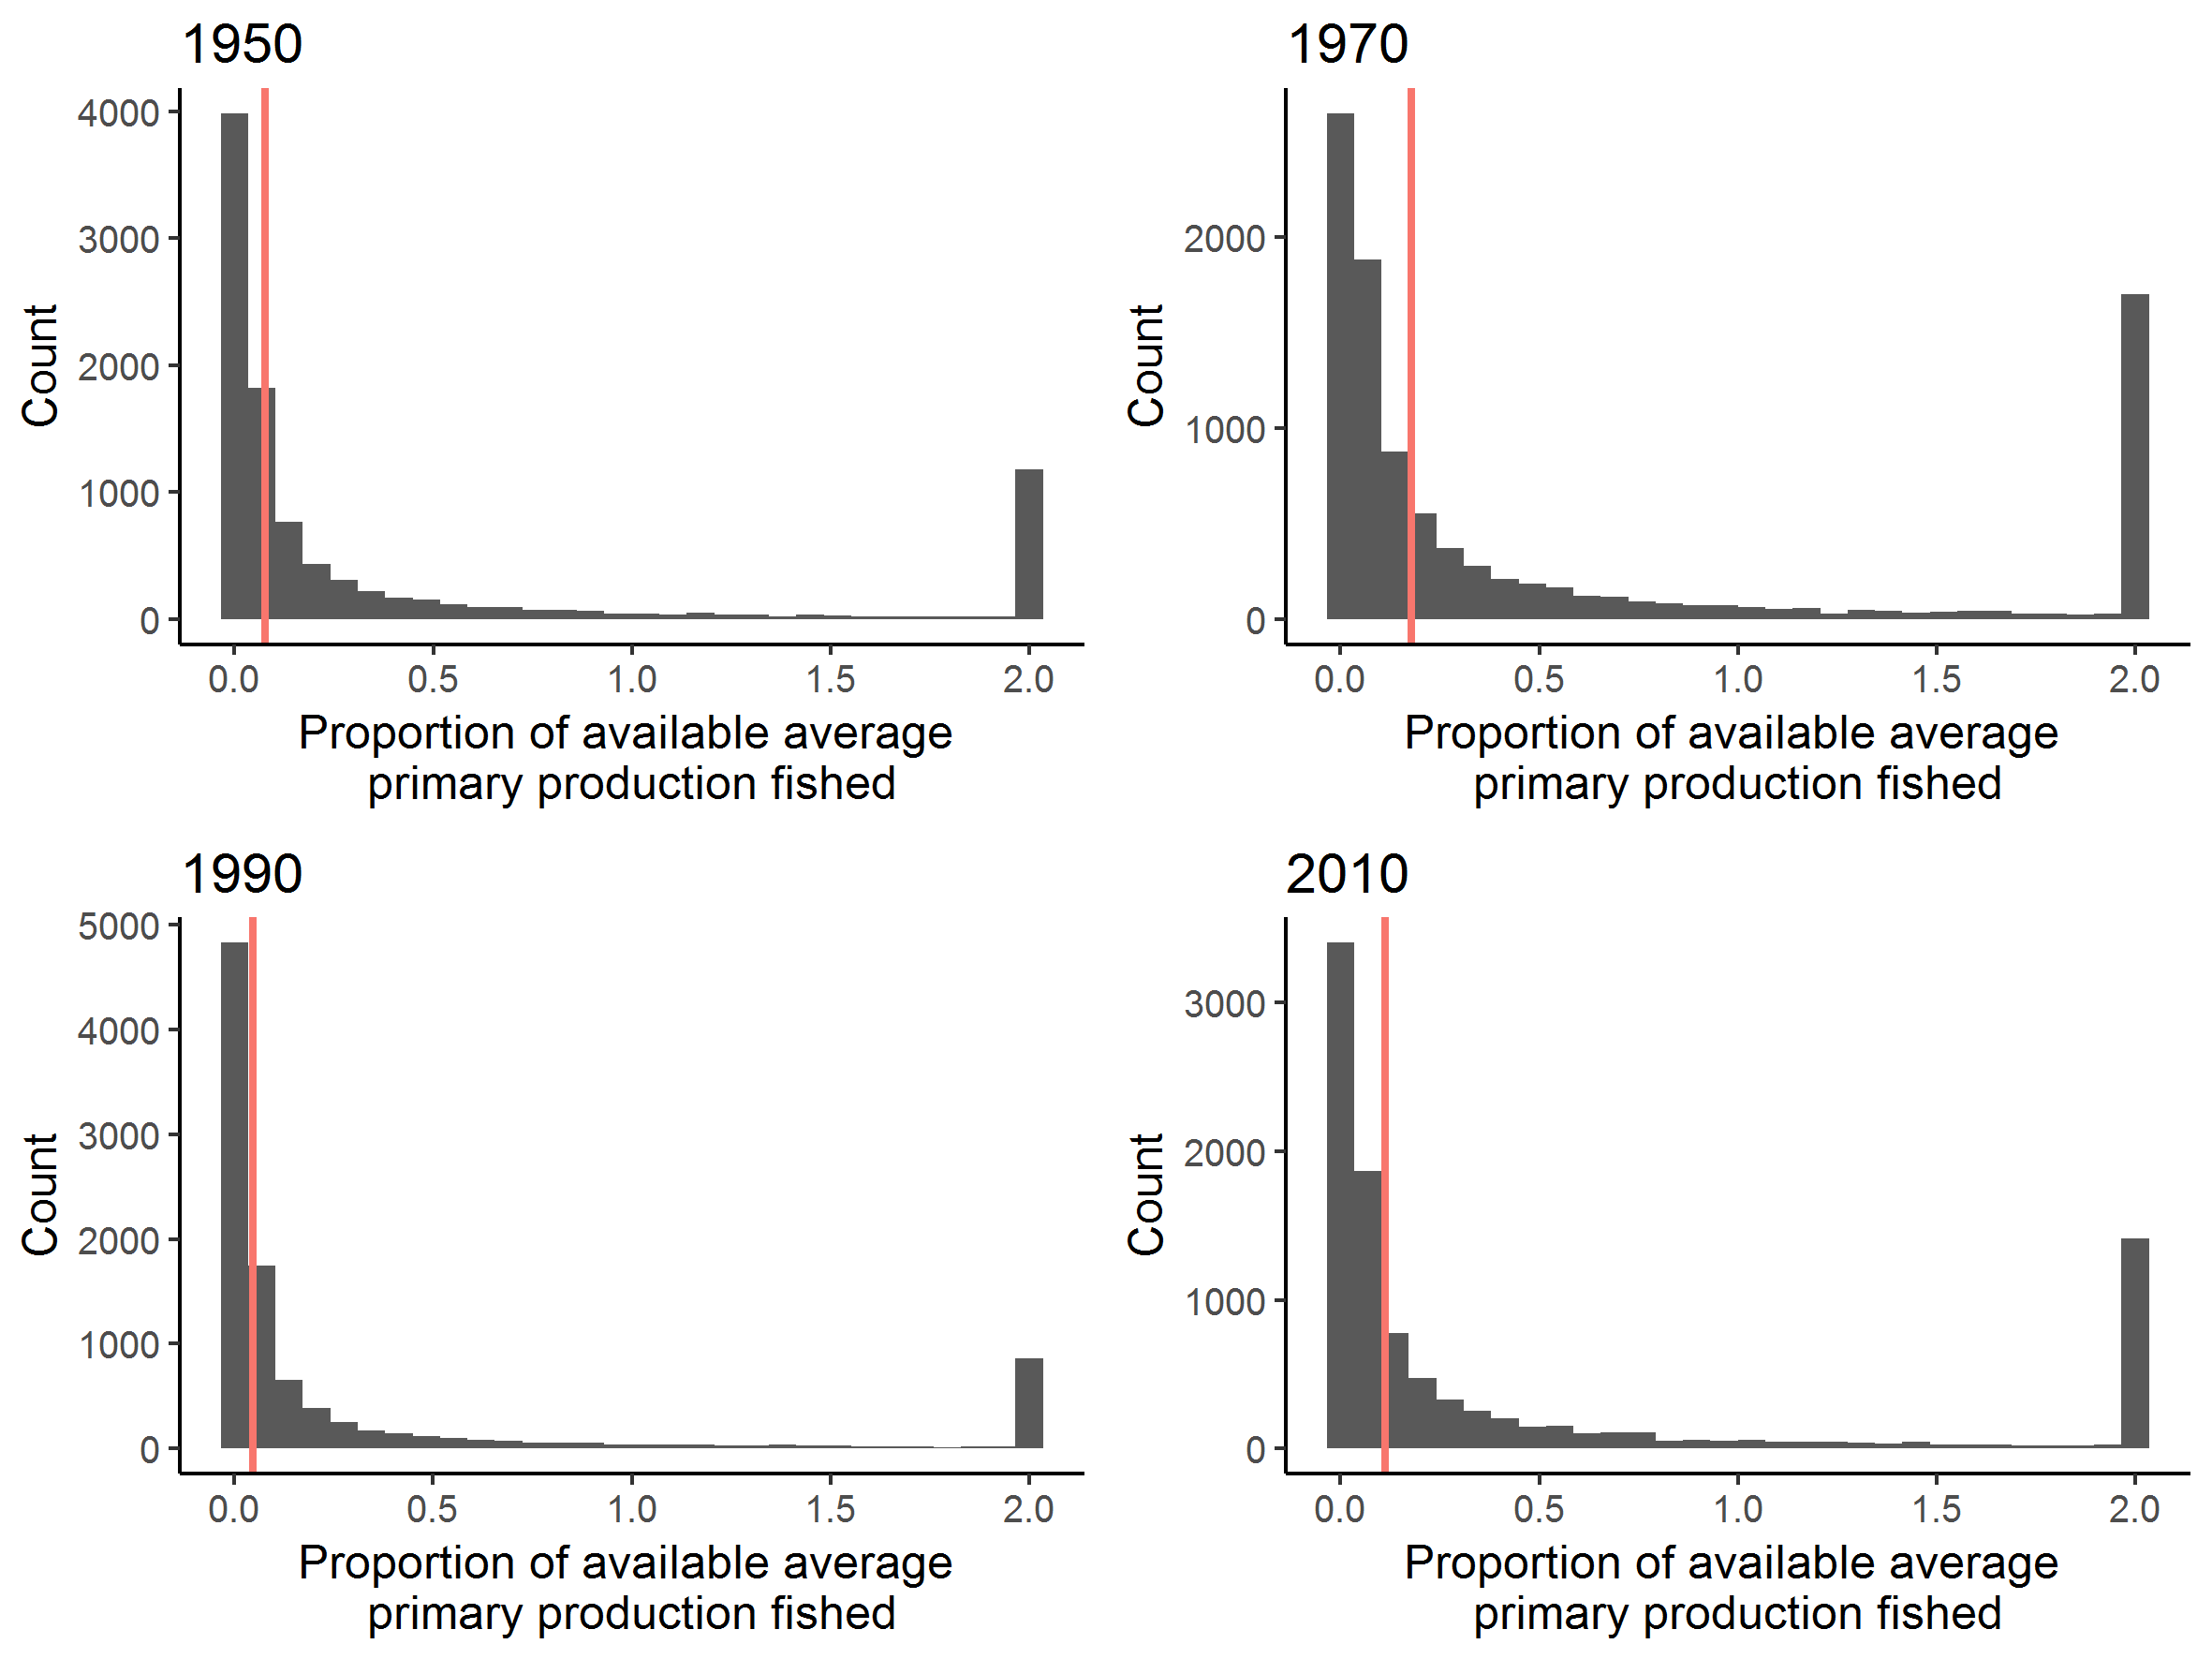
\includegraphics[width=.8\textwidth]{fig/hist_pp_1950_2010}
    \caption{Histogram of simulated primary production required given catch divided by the average primary production in 1950, 1970, 1990, and 2010 in the California Current using a random transfer efficiency. The vertical red line indicates the primary production required divided by primary production using a fixed 10\% transfer efficiency in the calculations. We adjusted the far right bin width due to rare events. The original range extends out further. Plot created using R v.3.4.3 \cite{Rcite} ggplot2 package v.2.2.1 \cite{ggplot}. }
    \label{ppr}
\end{figure}

\subsection{Applications in Aquaculture}
Aquaculture already cultivates hundreds of different marine and freshwater species. The relevance of transfer efficiencies to production decisions depends on whether the species requires additional feed or not. Non-fed aquaculture includes either primary producers or primary consumers that are not provided additional feeds by the aquaculturist. Fed aquaculture, on the other hand, involves consumer species that are typically fed compound feeds designed to meet their specific nutritional requirements. Consumption of autotrophs, usually phytoplankton by filter feeders, is studied extensively in non-fed aquaculture to track carrying capacity of ecosystems with added aquaculture \cite{banas2007tidal}. These carrying capacities are estimated using assimilation efficiencies of a specific target species \cite{rosland2009applying, irisarri2013absorption, srisunont2016estimating} or as broader estimates of transfer efficiencies \cite{simenstad1995influence, sommer1998algal, byron2011calculating, han2017evaluating}.

\vspace{5mm}

More and more fed species are given specialized compound feeds rather than whole organisms in order to increase efficiency and sustainability of feed resources. To assess the sustainability of feeds, the field has begun to track transfer efficiencies by dissecting the feed into its compositional parts and estimating the efficiencies for each of the components using the method devised by \citet{pauly1995primary}. While a 10\% transfer efficiency was initially employed to estimate the primary production requirements or biotic resource use in environmentally-based aquaculture assessments (e.g., \citealt{papatryphon2004environmental, pelletier2007feeding, pelletier2009not}), more recent studies have incorporated species-specific efficiencies in their analyses to better understand the environmental tradeoffs between different feed compositions \cite{cashion2016review}. Additionally, \citet{cashion2016review} found that the use of a 10\% transfer efficiency has led to an underestimation of the impacts of salmon aquaculture on natural marine biomass resources. Actual impacts are likely three times greater. As with the case for wild fisheries, ignoring the variability in transfer efficiencies can have negative impacts on the conservation of limited resources and management of human activities.

\section{Concluding Remarks}
Our results raise the question why the use of an assumed transfer efficiency value of 10\% is still so prevalent despite widespread evidence of substantial variability and examples of where the consequences of ignoring such variability have been documented? One issue is clearly convenience. The overall mean of observed values is not dramatically different from the assumed 10\% value. Nonetheless, given the scope of observed variation and uncertainty, using a 10\% value for the sake of arithmetic convenience carries large risks. Our study is not the first to raise this point, but synthesizing the full scope of evidence around the levels of variability and its potential consequences for decisions will hopefully highlight the costs of ignoring variability in this key ecosystem parameter. 

\vspace{5mm}

Another reason for the continued assumption of a constant value is the lack of relevant data for most systems. But our synthesis of the distributions of observed values for trophic efficiency in freshwater and marine ecosystems provides an opportunity to draw from this synthetic distribution rather than assuming a constant value. In cases where locally relevant data are infeasible to collect, this synthetic distribution may provide a better platform for decisions. 

\vspace{5mm}

Finally, one other issue is that the studies that have addressed the variability in transfer efficiency specifically have typically been in the context of narrower questions (e.g., aquaculture feeds). These narrower studies may not catch the attention of people using transfer efficiencies in other ways. By pulling together information from diverse studies from different fields, we hope this synthesis will generate a broader discussion.

\vspace{5mm}

In the absence of specific data for a broader array of systems, instead of using a fixed 10\% constant, we suggest using simulations or Bayesian models drawing on these synthetic distributions, which are great tools for incorporating variation and uncertainty. This approach would take us a long ways towards creating more valid food web models, and as such, improve our understanding on how food web dynamics impact community structure. 


%=== Chapter 2  ============================================
\chapter{Untangling uncertainty in food web models}
%---  Introduction -------------------------

\section*{Introduction}
Many managed fisheries constitute data-limited cases \cite{farmer2016stock} where there is insufficient information to evaluate population health and the sustainability of fishing practices with a full stock assessment. One common approach to overcome data limitations has been to aggregate multiple species together into stock complexes and create a single aggregate population dynamic model for the group \cite{cope2011approach}. Typically, similar species, or the species that are targeted together by the same fleets, are aggregated into a common model. However, this approach is based on strong assumptions which can compromise the validity or interpretability of the model results. 

\vspace{5mm}

Perhaps the largest limitation to using a species complex model is that clustering species leads to a loss of information at the individual-species level. This is especially true when aggregated complexes are assessed using simple biomass dynamics models. In those cases the aggregated species are assumed to share life history traits (e.g., carrying capacity, expected lifespan, growth rates, reproductive rates, etc.), geographical ranges, and vulnerabilities. Ignoring the potential differences in vulnerabilities and sensitivities to fishing pressure is a serious concern when modeling species together as a complex and can lead to inaccurate and unsustainable predictions of biomass for some or all the stocks. Catch levels set to maximize one species could drive a ``weaker stock" to  unsustainably low levels \cite{hastings2017marine}.

\vspace{5mm}

Traditional single-species assessment modeling estimates the impacts of fishing using fisheries-related data such as catch, composition of the catch, and indices of abundance. These single-species models often lack the capability to incorporate broader-scale ecosystem information. Food web models, which are a type of ecosystem-based model, are capable of providing estimates of quantities such as carrying capacity, tropic level abundance, and transfer rates that are conceptually similar to concepts of single-species assessment modeling of carrying capacity, abundance, and intrinsic rates of increase. Incorporating ecosystem concepts into single-species assessments may offer a way forward for data-limited situations as well as provide a pathway from single-species to ecosystem-based management.

\vspace{5mm}

A problem in incorporating ecological concepts into statistical models of applied fisheries assessments is the quantification of uncertainty. Fisheries models are increasingly using state-space modeling approaches and with that comes an array of possibilities. Measures of the confidence in model results are important in setting management decisions. Most existing food web models are deterministic (do not take into account variation). A way of incorporating uncertainty in models is through simulation. We developed an approach using trophic pyramid food webs combined with Monte Carlo simulations to simulate values of trophic level biomass under different ecological assumptions. By considering uncertainty under different scenarios, we are able to quantify parameter and model output uncertainties in a way that has not previously been done in existing ecosystem models. 

\vspace{5mm}

Applying this technique on a data-limited fishery gives insight into the rigor of information we can expect to obtain when ecological concepts are incorporated into fisheries models and from there, how this information can be applied in fisheries assessments. The past few assessments of the main Hawaiian Islands Deep7 Bottomfish Complex groundfish fishery used an aggregate surplus production model for the complex. However there is a concern that life history traits may differ amongst the targeted species, which could ultimately affect the vulnerability to fishing pressure \cite{brodziak2011stock, langseth2018stock}. We used the main Hawaiian Islands (MHI) as the setting for our simulations to not only gain insight on the fishery and region, but to also minimize assumptions in our model construction, particularly those related to the movement of migratory species and larval dispersal. We needed to select a marine ecosystem that was as close to a naturally closed system as possible. Hawaii does not lie directly in the path of any current system, and the local wind and current patterns create a system of cyclonic eddies. Due to these properties, prior studies concluded that there is an oceanic barrier to larval dispersal \cite{lobel1986transport, vermeij1987dispersal, hourigan1987mid}. Therefore, we considered the MHI a naturally enclosed marine ecosystem due to the containment of larval drift.


\section*{Methods}
\subsection*{Base Equation}
Both \citet{lalli1997biological} and \citet{libralato2008novel} outlined that production at each trophic level ($h$) can be estimated from net primary production  (NPP, denoted $\nu$) multiplied by the trophic transfer efficiencies ($\tau_h$). In line with extant research on this topic (see \citealt{cury2005trophodynamic, libralato2008novel, chassot2010global, trebilco2013ecosystem, watson2014primary}) we define the transfer efficiency ($\tau_h$) as the fraction of production passing from trophic level $h-1$ to $h$, where $h$ is the higher trophic level in the food web. In many cases net primary production is represented in metric tons C/year and is multiplied by 9 to convert from organic carbon (metric tons C) to wet weight (metric tons) \cite{strathmann1967estimating, pauly1995primary, chassot2010global}. We include the lifespan term $\lambda_h$ to convert from the weight of individuals produced in a year to the overall standing stock in Eq. (\ref{base}) as we are interested in solving for trophic level biomass ($\gamma_h$) instead of production. See Table \ref{description} for defined variables and parameters definitions within Eq. (\ref{base}).

\begin{equation} \label{base}
\gamma_h = \nu * 9 * \left( \prod_{j=2}^{h} \tau_j \right) \lambda_h \hspace{5mm} \text{for} \hspace{5mm} h \in \{2, 3, 4\}
\end{equation}

\begin{table}[H]
\centering
\caption{Definition of notation in Eq. (\ref{base}) and scientific units used}
\begin{tabular}{l|l|l}
  \hline \small
 Terms & Description & Units  \\ 
   \hline
   $h$ & Trophic level in MHI, where $h = 2,3,4$  & \\
   $\gamma_h$ &  Trophic level biomass at trophic level $h$ & metric tons  \\
   $\nu$ & NPP & metric tons C/year \\
   9 & Carbon to wet weight conversion ratio & metric tons/metric tons C \\
   $\tau_{h}$ & Transfer efficiency between trophic level $h-1$ and $h$ &   \\  
   $\lambda_h$ & Lifespan of a species found at trophic level $h$ & years \\
   \hline
\end{tabular} 
\label{description}
\end{table}

\subsection*{Data}
We built Eq. (\ref{base}) for our case study of the MHI using the following data sources: We used the 8-day time series Sea-viewing Wide Field-of-view Sensor (SeaWiFS) chlorophyll \textit{a} data from 1997 to 2010 that was transformed using the \textit{Eppley-}Vertically Generalized Production Model (VGPM) to estimate NPP from chlorophyll \textit{a} from the Ocean Productivity group at Oregon State University (\url{http://www.science.oregonstate.edu/ocean.productivity/}) (Fig. \ref{SeaWiFSmhi}) \cite{behrenfeld1997photosynthetic}. Estimated trophic levels (rational numbers) were calculated from the FishBase database (\url{http://www.fishbase.org/}) of \citet{fishbase} for each species and truncated to assign species into integer-valued trophic levels. Truncated trophic levels range in the MHI from $h=1,\dots,4$ with $h=1$ representing phytoplankton, $h=2$ primary consumers, $h=3$ secondary consumers, and $h=4$ tertiary consumers. In this ecosystem, the maximum trophic level is 4. However, this value can vary in other ecosystems depending on the species composition. The \citet{fishbase} FishBase data set was also used to estimate the lifespan ($\lambda_h$) across all species at trophic level $h$. In this database \citet{fishbase} defines the term lifespan as ``the maximum expected age, on average, for a species, cohort, stock, or a population in the absence of fishing. Smaller than maximum age although may be used in this sense."

\begin{figure}[H]
     \centering
       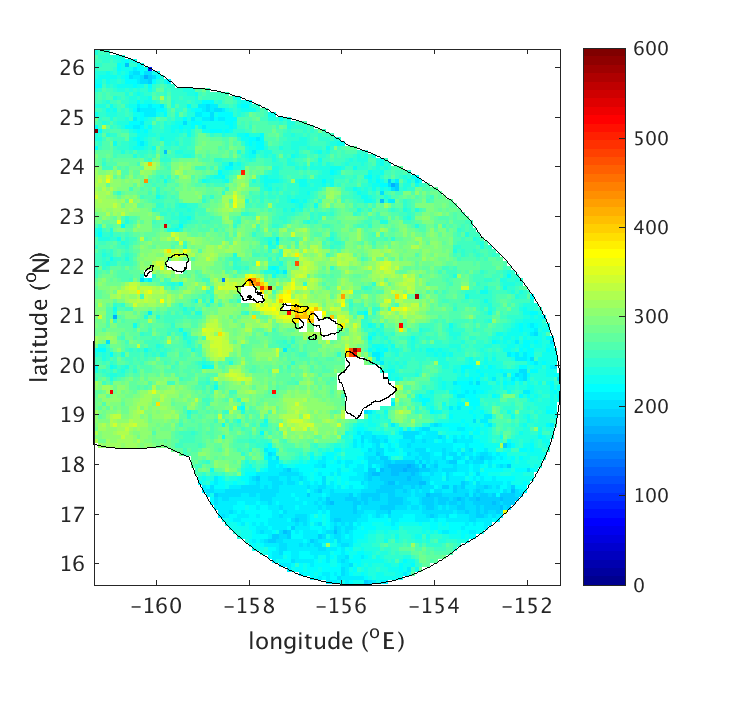
\includegraphics[width=.7\textwidth]{fig/SeaWiFSmhi}
    \caption{A single 8-day time frame of the SeaWiFS \textit{Eppley-}VGPM NPP data in January 1998 for the main Hawaiian Islands EEZ. The color scale shows the amount of estimated NPP in total gigatons of Carbon per year per pixel. The pixel size of the SeaWiFS data set is 9 by 9 km. Image created by Erik Fields (Earth Research Institute, ERI).}
    \label{SeaWiFSmhi}
\end{figure}

\subsection*{Assumptions and General Model}
\subsubsection*{Assumptions in Model}
In Eq. (\ref{joint}), we present the decomposition of the joint distribution for the general ecological model. Here we assume that the random variables NPP $(\nu)$, transfer efficiencies $(\tau_2, \tau_3,$ and $\tau_4)$, and lifespans $(\lambda_2, \lambda_3,$ and $\lambda_4)$ are independent. This assumption is ecologically reasonable, because the amount of energy going into the system does not depend upon the transfer of energy or an organism's lifespan. Additionally, we assume that the distribution of transfer efficiency at trophic level $h$, ($\tau_h$), is independent of transfer efficiency at the previous trophic level ($\tau_{h-1}$). Throughout this paper, we therefore assume the joint distribution for $\nu, \tau_2, \tau_3, \tau_4, \lambda_2, \lambda_3,$ and $\lambda_4$ can be broken down as:

\begin{equation} \label{joint}
f(\nu, \tau_2, \tau_3, \tau_4, \lambda_2, \lambda_3, \lambda_4) =  f(\nu)f(\tau_2)f(\lambda_2)f(\tau_3)f(\lambda_3)f(\tau_4)f(\lambda_4)  
\end{equation}

Since the trophic level biomass, $\gamma_h$, for trophic levels $h \in \{ 2,3,4\}$ in Eq. (\ref{base}) is a deterministic function of the random variables from Eq. (\ref{joint}), given the distributional assumptions detailed both above and in Table \ref{assumcases}, it is possible  in some cases to find the distribution of $\gamma_h$ for $h \in \{2, 3, 4\}$. Our assumptions in Eq. (\ref{joint}) implies that we are assuming if trophic level $h_x$ does not equal to trophic level $h_y$, the lifespan ($\lambda_{h_{x}}$) is independent of trophic level biomass ($\gamma_{h_{y}}$) for $h_x, h_y \in \{2, 3, 4\}$.

\subsubsection*{Random Distributions on Random Variables}
Variation in ecosystem-based models is a contested area of research in fisheries science. Many studies use a default 10\% transfer efficiency for $\tau_h$ for each $h \in \{2, 3, 4\}$ (i.e., $\tau_h = 0.10 \hspace{2mm} \forall \hspace{2mm} h \in \{2, 3, 4\}$), thereby assuming this is constant across all trophic levels \cite{lindeman1942trophic, slobodkin1962energy, may1976theoretical, pauly1995primary}. However, other researchers have estimated that the true transfer efficiency may be higher than 10\% \cite{schaefer1965potential, ryther1969photosynthesis,sheldon1977structure, baumann1995comment}, may vary depending on the size and type of ecosystem \cite{libralato2008novel, heymans2011ecopath}, and decrease with increasing trophic levels \cite{may1983ecology, barnes2010global}. As the current study is applied to a data-limited case, we are unsure of the values of NPP ($\nu$), transfer efficiency $(\tau_h)$, and lifespans ($\lambda_h$) for $h \in \{2, 3, 4\}$ in the model. Therefore, we choose to study sensitivities of biomass ($\gamma_h$) to each of the three components.

\subsubsection*{Distributional Assumptions}
Several distributional and conditional assumptions we placed on the distributions of the random variables NPP ($\nu$), transfer efficiencies $(\tau_h)$, and lifespans ($\lambda_h$) for $h \in \{2, 3, 4\}$ are described in Table \ref{assumcases} and visualized in Fig. \ref{distassump} as special cases of our general model Eq. (\ref{joint}). In Case 1 of $f(\nu)$, a value of $c_1 = 87339861.7$ metric tons C/ year was estimated by fitting a time series seasonal autoregressive integrated moving average model (SARIMA model) to the SeaWiFS data using R v.3.4.3 \cite{Rcite} forecast package v8.2 and function auto.arima() \cite{forecast1, forecast2}. Case 2 of $f(\nu)$ was approximated based on goodness-of-fit tests fitted to the SeaWiFS data \cite{fitdistrplus} (Fig. \ref{distassump}). 

\vspace{5mm}

We based the distributional assumptions for Case 1 of the transfer efficiencies $\tau_h$ for $h \in \{2, 3, 4\}$ from \citet{pauly1995primary}. We used \citet{pauly1995primary} average transfer efficiency value of 0.1013 for $c_2$ in our study. We utilized data gathered from a meta analysis on marine transfer efficiencies to fit approximate distributions based on goodness-of-fit tests \cite{fitdistrplus} for Case 2 and 3 of the transfer efficiencies $\tau_h$ (Fig. \ref{distassump}). Case 2 has the transfer efficiency ($\tau_h$) come from the same distribution for all $h \in \{2, 3, 4\}$, while Case 3 places distinct distributions on each transfer efficiency.

\vspace{5mm}

In Case 1 for $f(\lambda_2)$, $f(\lambda_3)$, and $f(\lambda_4)$, the values of $c_3=5.75$ years, $c_4=6$ years, and $c_5=11.95$ years were calculated by taking the median of the maximum expected lifespan data at each trophic level $h$. When lifespans ($\lambda_h$ for $h \in \{2, 3, 4\}$) are treated as random variables (non-constant), we chose approximate distributions based on goodness-of-fit tests \cite{fitdistrplus} (Fig. \ref{distassump}). Details of the SARIMA model and the steps taken to estimate the parameters in the Lognormal and Beta distributions in Table \ref{assumcases} are in Appendix \ref{appendix:b}.
   
\begin{table}[H]
\centering
\caption{Distributional assumption cases are special cases for the components of the joint distribution (i.e., Eq. (\ref{joint})). We treat $c_1$, $c_2$, $c_3$, $c_4$, and $c_5$ as constants.  Lack of subscripts means the parameter has the same value across all distributions.}
\begin{tabular}{|c|c|c|c|}
  \hline 
 	& Case 1 & Case 2 & Case 3  \\ 
   \hline
   \multirow{2}{*}{$f(\nu)$} 	& 1 if $\nu = c_1$ & 
   \multicolumn{2}{c|}{ \multirow{2}{*}{$Lognormal(\mu_\nu, \sigma_\nu^2)$ }} \\
   				& 0 else 			 & 	\multicolumn{2}{c|}{ } \\
   \hline   
   \multirow{2}{*}{$f(\tau_2)$} & 1 if $\tau_2 = c_2$ & \multirow{2}{*}{$Beta(\alpha, \beta)$} & \multirow{2}{*}{$Beta(\alpha_{\tau_2}, \beta_{\tau_2})$}  \\
         			& 0 else &  &  \\
   \hline   
   \multirow{2}{*}{$f(\tau_3)$}  & 1 if $\tau_3 = c_2$ & \multirow{2}{*}{$Beta(\alpha, \beta)$} & \multirow{2}{*}{$Beta(\alpha_{\tau_3}, \beta_{\tau_3})$}  \\
            			& 0 else & &  \\
   \hline  
   \multirow{2}{*}{$f(\tau_4)$} & 1 if $\tau_4 = c_2$ &  \multirow{2}{*}{$Beta(\alpha, \beta)$} & \multirow{2}{*}{$Beta(\alpha_{\tau_4}, \beta_{\tau_4})$}  \\
               			& 0 else & &  \\
   \hline      	
    \multirow{2}{*}{$f(\lambda_2)$} & 1 if $\lambda_2 = c_3$ & \multicolumn{2}{c|}{\multirow{2}{*}{$Lognormal(\mu_{\lambda_2}, \sigma_{\lambda_2}^2)$}} \\
    	& 0 else	& 	\multicolumn{2}{c|}{ }  \\
   \hline      	
    \multirow{2}{*}{$f(\lambda_3)$} & 1 if $\lambda_3 = c_4$ & \multicolumn{2}{c|}{\multirow{2}{*}{$Lognormal(\mu_{\lambda_3}, \sigma_{\lambda_3}^2)$}} \\
    	& 0 else	& 	\multicolumn{2}{c|}{ }  \\
   \hline      	
    \multirow{2}{*}{$f(\lambda_4)$} & 1 if $\lambda_4 = c_5$ & \multicolumn{2}{c|}{\multirow{2}{*}{$Lognormal(\mu_{\lambda_4}, \sigma_{\lambda_4}^2)$}} \\
    	& 0 else	& 	\multicolumn{2}{c|}{ }  \\    	
   \hline
\end{tabular} 
\label{assumcases}
\end{table}

\begin{figure}[H]
     \centering
       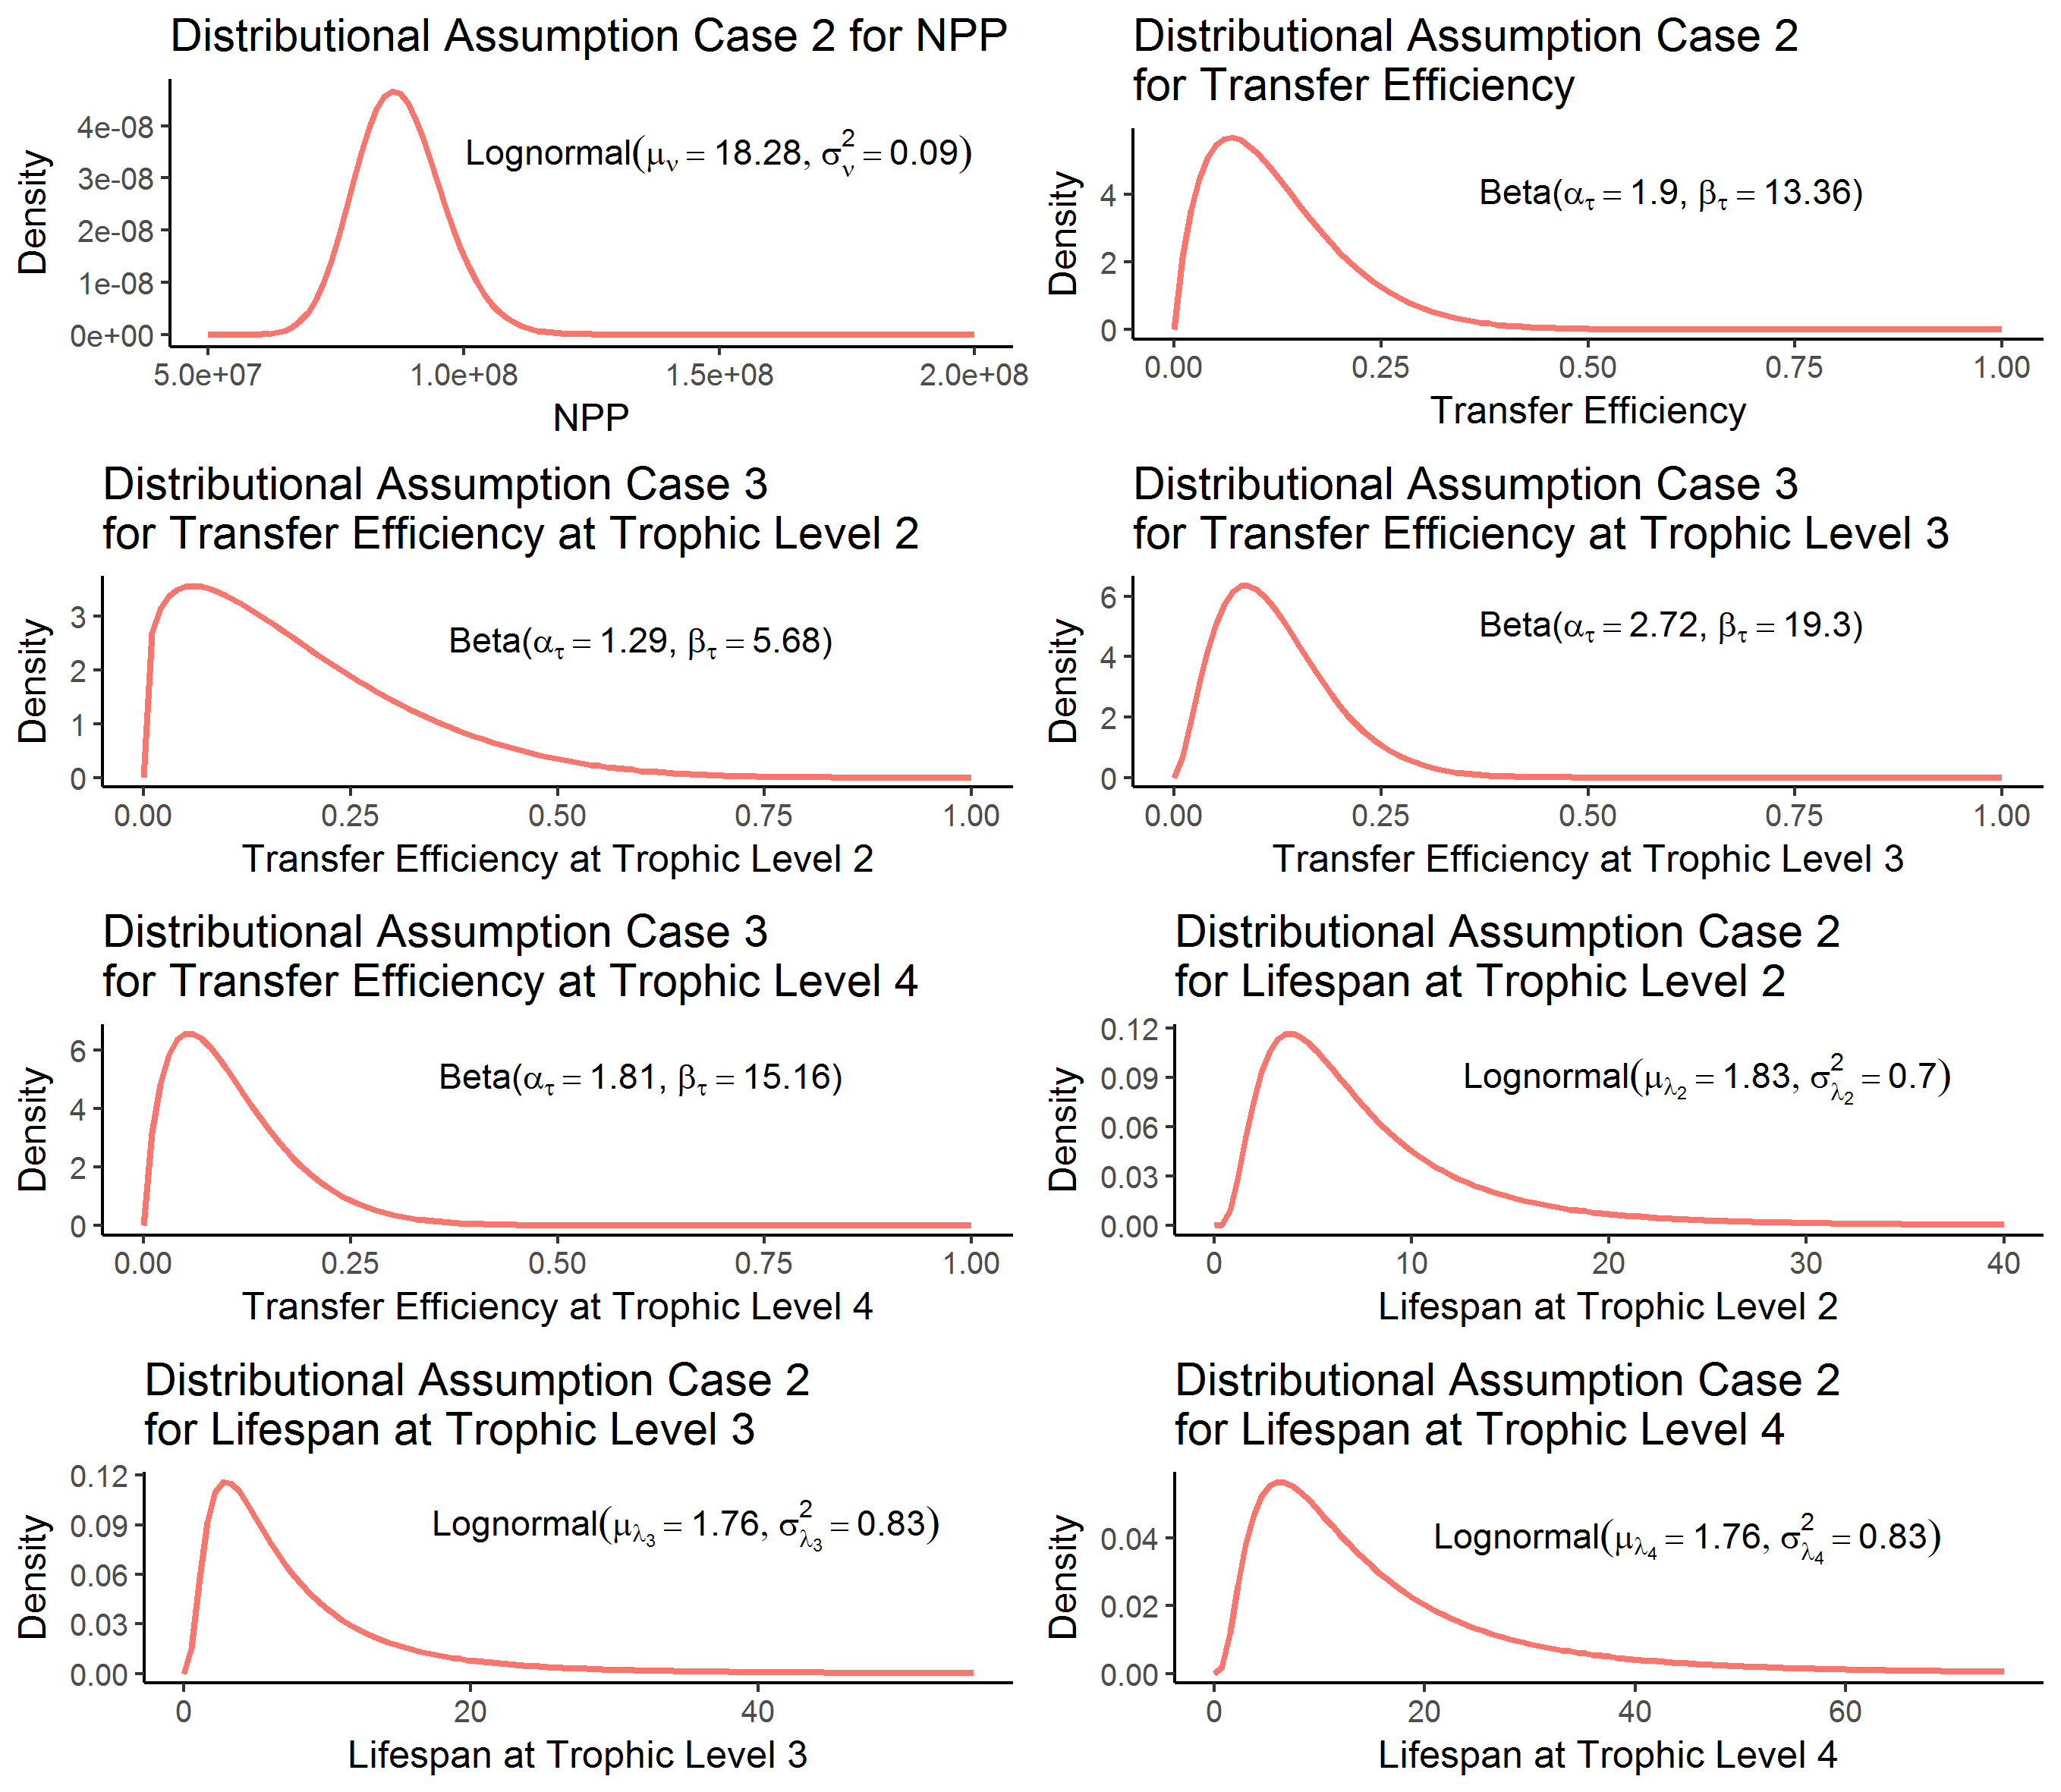
\includegraphics[width=.9\textwidth]{fig/distassump}
    \caption{Probability distributions for the distributional assumption cases described in Table \ref{assumcases} where NPP ($\nu$), transfer efficiencies ($\tau_h$ for $h \in \{2, 3, 4\}$), and lifespans ($\lambda_h$ for $h \in \{2, 3, 4\}$) are not fixed values. Plot created using R v.3.4.3 \cite{Rcite} ggplot2 package v.2.2.1 \cite{ggplot}. }
    \label{distassump}
\end{figure}

\subsection*{Simulation Scenarios}
We combine distributional assumptions on the components of Eq. (\ref{joint}) corresponding to NPP $f(\nu)$, transfer efficiencies $f(\tau_h)$, and lifespans $f(\lambda_h)$ for $h \in \{2, 3, 4\}$ from Table \ref{assumcases} to create different scenarios that represent various ecological assumptions (See Table \ref{scenariosids} for the explanation of scenario code names and Table \ref{scenarios} for description of scenarios). In Table \ref{scenarios}, we interpret each cell as the $i^{th}$ distributional case outlined in Table \ref{assumcases} for the $x^{th}$ variable. For example, we would interpret $f^1(\nu)$ as the distributional assumption under the column Case 1 for $f(\nu)$ in Table \ref{assumcases}. The transfer efficiencies ($\tau_2, \tau_3, \tau_4$) and maximum expected lifespans ($\lambda_2, \lambda_3, \lambda_4$) are independent of each other in all cases. We construct different scenarios to not only incorporate uncertainty in the NPP (denoted by superscript ``2" in Table \ref{assumcases}, $f^2(\nu)$) and lifespans ($f^2(\lambda_h)$ for $h \in \{2, 3, 4\}$), but also to encompass contrasting values for the transfer efficiency. The three areas focused on in this manuscript are: constant transfer efficiencies ($f^1(\tau_h)$ for $h \in \{2, 3, 4\}$), non-constant but independent transfer efficiencies ($f^2(\tau_h)$ for $h \in \{2, 3, 4\}$), and the constriction on transfer efficiencies distributions at successive trophic levels ($f^3(\tau_h)$ for $h \in \{2, 3, 4\}$). Scenario NTL (i.e., fixed NPP ($\nu$), fixed transfer efficiencies ($\tau_h$), and fixed lifespans ($\lambda_h$)) is a simplistic model intended to be used as a comparison to other relatively similar simple equations \cite{pauly1995primary, cury2005trophodynamic, chassot2010global, watson2014primary}. 

\begin{table}[H]
\centering
\caption{Key of the scenario code names used to identify the various ecological and distributional assumptions.}
\begin{tabular}{|c|cc|cc|cc|}
  \hline Types of Transfer Efficiency & \multicolumn{2}{c|}{NPP ($\nu$)} & \multicolumn{2}{c|}{Transfer efficiency ($\tau_h$)}  &  \multicolumn{2}{c|}{Lifespan ($\lambda_h$)}  \\ 
  Variation & Fixed & Random & Fixed & Random & Fixed & Random  \\
    \hline
  Fixed 10\% & N & n & T &   & L & l \\
  Allowed to vary & \textit{N} & \textit{n} & & \textit{t} & \textit{L} & \textit{l} \\
  Decreases as move up food web & \textbf{N} & \textbf{n} & & \textbf{t} & \textbf{L} & \textbf{l} \\
  \hline
\end{tabular} 
\label{scenariosids}
\end{table}

\begin{table}[H]
\centering
\caption{Scenarios are combinations of the distributional assumption cases described in Table \ref{assumcases}, where $f^i(x)$ indicates the $i^{th}$ distributional assumption for the variable $x$. Table \ref{scenariosids} defines the code names for the scenarios. }
\begin{tabular}{|c|c|c|c|c|c|}
  \hline \small
   Scenarios & $f(\nu)$ & $f(\tau_2)$ & $f(\tau_3)$ & $f(\tau_4)$ & $f(\lambda_h)$  \\ 
  \hline
  NTL & $f^1(\nu)$ & $f^1(\tau_2)$ & $f^1(\tau_3)$ & $f^1(\tau_4)$ & $f^1(\lambda_h)$ \\
  NTl & $f^1(\nu)$ & $f^1(\tau_2)$ & $f^1(\tau_3)$ & $f^1(\tau_4)$ & $f^2(\lambda_h)$ \\
  nTl & $f^2(\nu)$ & $f^1(\tau_2)$ & $f^1(\tau_3)$ & $f^1(\tau_4)$ & $f^2(\lambda_h)$ \\   
  \textit{NtL} & $f^1(\nu)$ & $f^2(\tau_2)$ & $f^2(\tau_3)$ & $f^2(\tau_4)$ & $f^1(\lambda_h)$ \\
  \textit{Ntl} & $f^1(\nu)$ & $f^2(\tau_2)$ & $f^2(\tau_3)$ & $f^2(\tau_4)$ & $f^2(\lambda_h)$ \\ 
  \textit{ntl} & $f^2(\nu)$ & $f^2(\tau_2)$ & $f^2(\tau_3)$ & $f^2(\tau_4)$ & $f^2(\lambda_h)$ \\
  \textbf{NtL} & $f^1(\nu)$ & $f^3(\tau_2)$ & $f^3(\tau_3)$ & $f^3(\tau_4)$ & $f^1(\lambda_h)$ \\
  \textbf{Ntl} & $f^1(\nu)$ & $f^3(\tau_2)$ & $f^3(\tau_3)$ & $f^3(\tau_4)$ & $f^2(\lambda_h)$ \\
  \textbf{ntl} & $f^2(\nu)$ & $f^3(\tau_2)$ & $f^3(\tau_3)$ & $f^3(\tau_4)$ & $f^2(\lambda_h)$ \\
  \hline
\end{tabular} 
\label{scenarios}
\end{table}

\subsection*{Simulation Details}
We were able to find equations for the distribution of $\gamma_h$ for $h \in \{2, 3, 4\}$ based on the transformation of parameters in Eq. (\ref{joint}) for Scenarios NTl and nTl. For details see Appendix \ref{appendix:b}. Given the current distributional assumptions placed on NPP ($f(\nu)$), transfer efficiencies ($f(\tau_h)$), and lifespans ($f(\lambda_h)$ for $h \in \{2, 3, 4\}$), we used simulations for the other six scenarios. Scenario NTL is a deterministic equation and therefore does not need simulation. We ran one million simulations for the other scenarios. 

\vspace{5mm}

In order to support simulation as a reasonable option, we examine the densities of Scenario NTl and nTl where we were able to derive the distributions of $\gamma_h$ and compare them to a version where we instead used simulations. We find that the analytical densities of the derived distributions and simulations are visually very similar to each other (Fig. \ref{scen1and4distsim}). 

\begin{figure}[H]
     \centering
       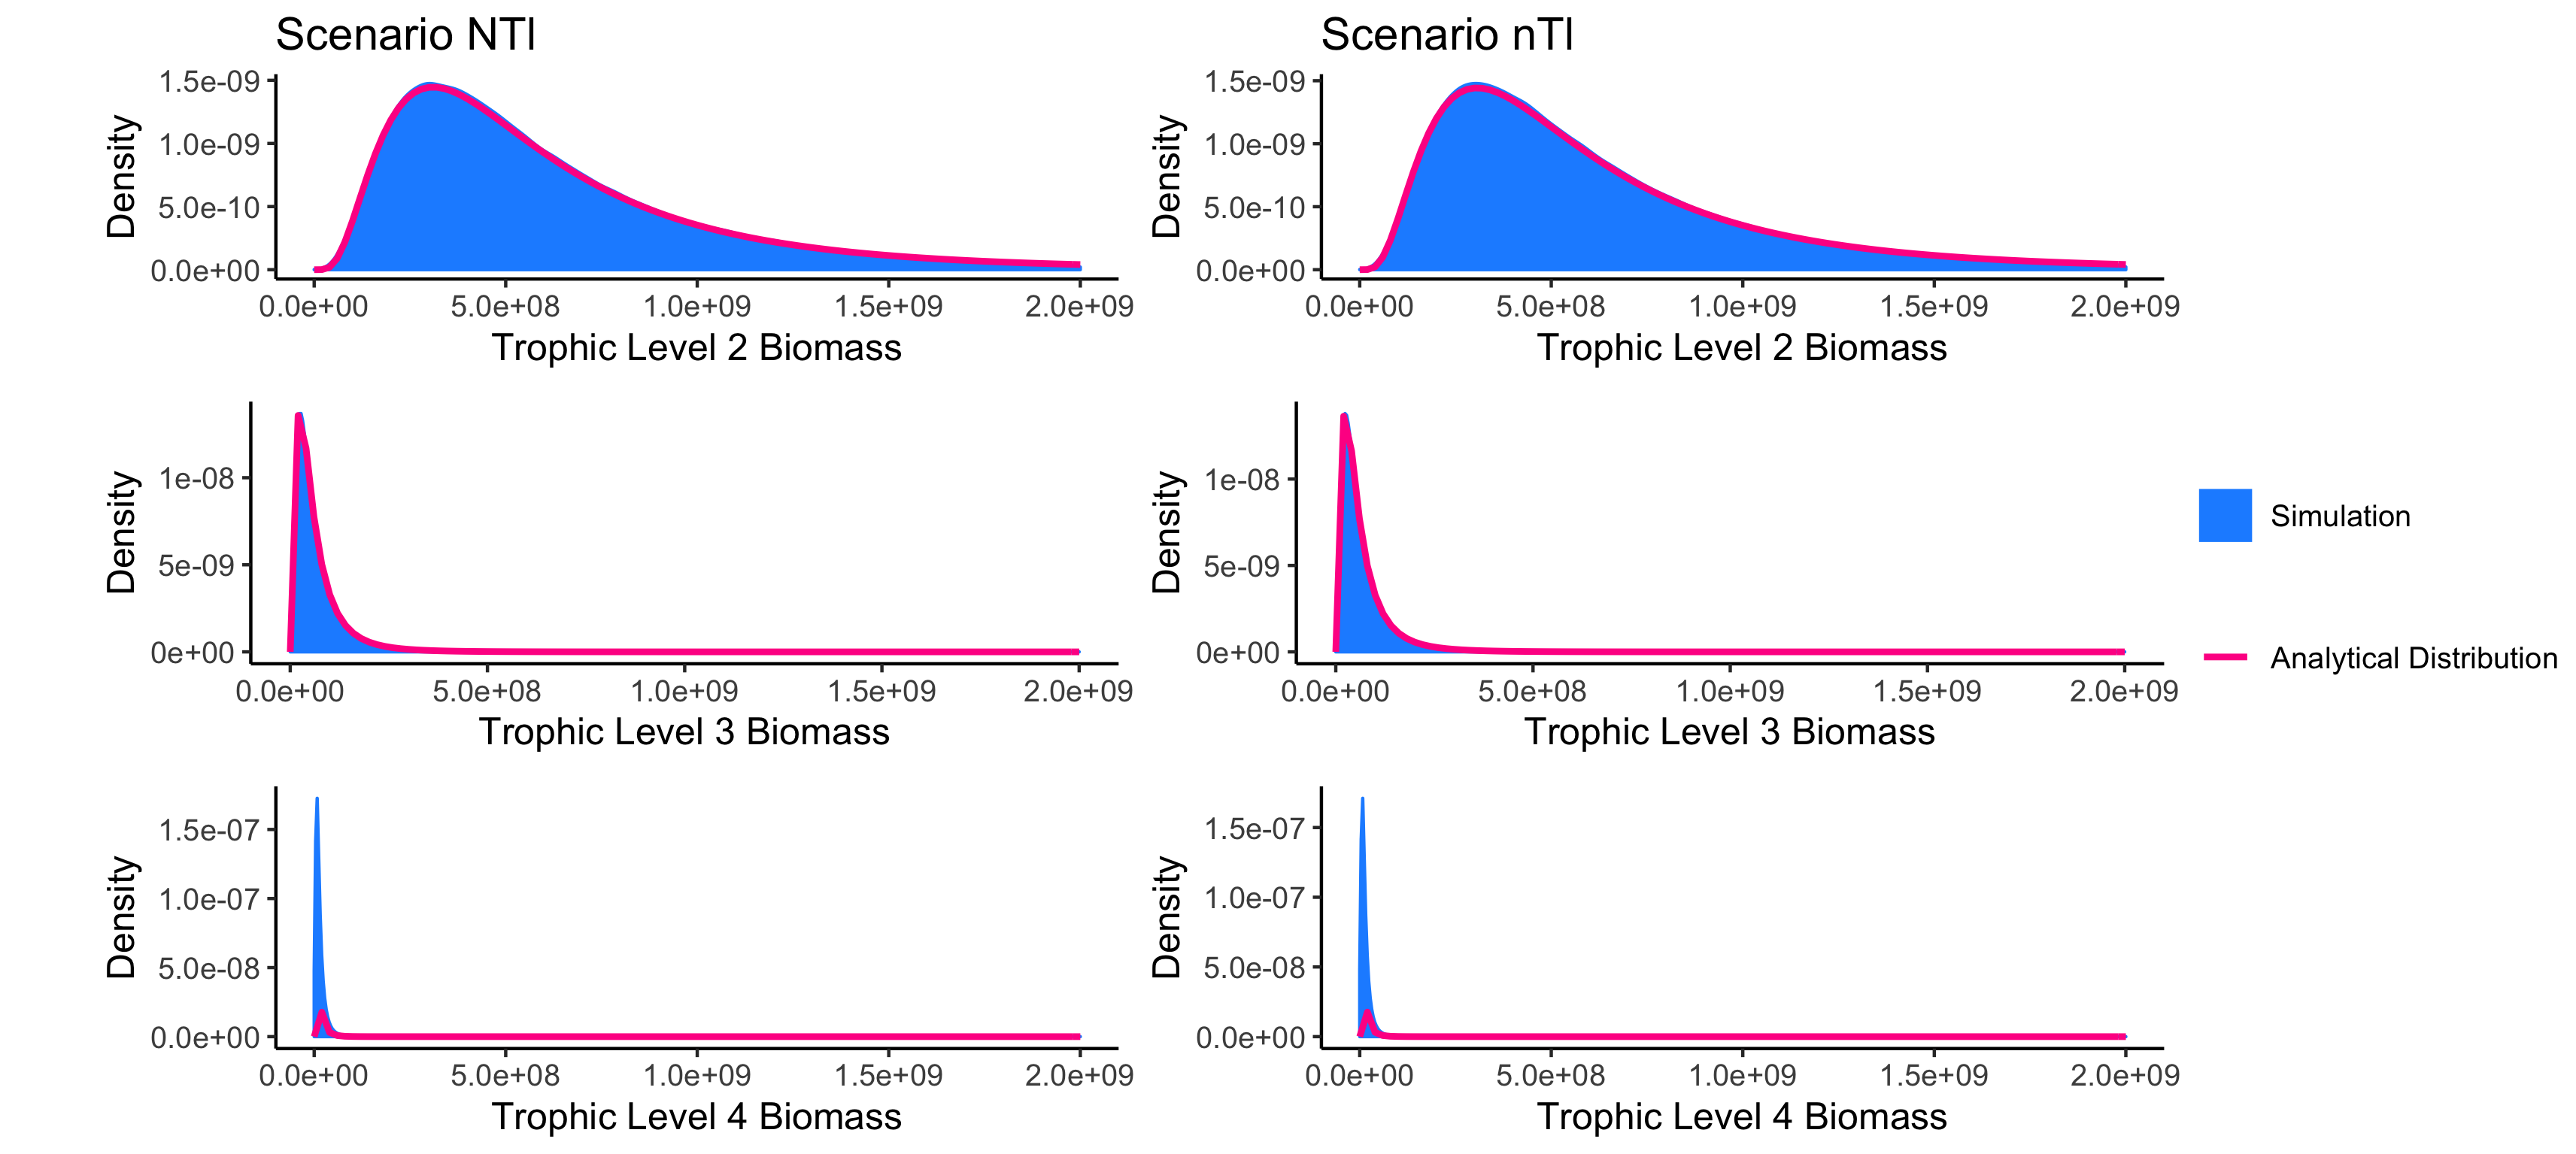
\includegraphics[width=\textwidth]{fig/scen4and7distsim}
    \caption{Comparison of the densities plots where we used simulations (blue) to the analytically derived probability distributions of $\gamma_h$ (pink line) in Scenarios NTl and nTl at each trophic level. We limited the upper bound of the x-axis to improve visualization. Plot created using R v.3.4.3 \cite{Rcite} ggplot2 package v.2.2.1 \cite{ggplot}. }
    \label{scen1and4distsim}
\end{figure}


\section*{Results}
At the primary consumer level ($h=2$), all scenarios exhibit skewed distributions of trophic level biomass ($\gamma_2$) (Fig. \ref{beta2estimated}). The peaks and tails of the biomass distributions are distinct amongst the scenarios with Scenarios \textbf{Ntl} and \textbf{ntl} having the fattest tails. When the transfer efficiency is treated as a random variable in Scenarios \textit{NtL}, \textit{Ntl}, \textit{ntl}, \textbf{NtL}, \textbf{Ntl}, and \textbf{ntl}, both the dispersion and interquartile ranges increase. Out of all of the scenarios, Scenarios NTl, nTl, \textit{NtL}, and \textbf{NtL} have the smallest coefficients of variation (CV) while Scenarios \textbf{Ntl} and \textbf{ntl} have the largest CV (Table \ref{cv}). The medians of the scenarios that represent the constricting distribution of transfer efficiencies as we move up the food web (i.e., \textbf{NtL}, \textbf{Ntl}, and \textbf{ntl}) are slightly higher than Scenario NTL's trophic level biomass estimate (Fig. \ref{beta2estimated}).   

\begin{figure}[H]
     \centering
       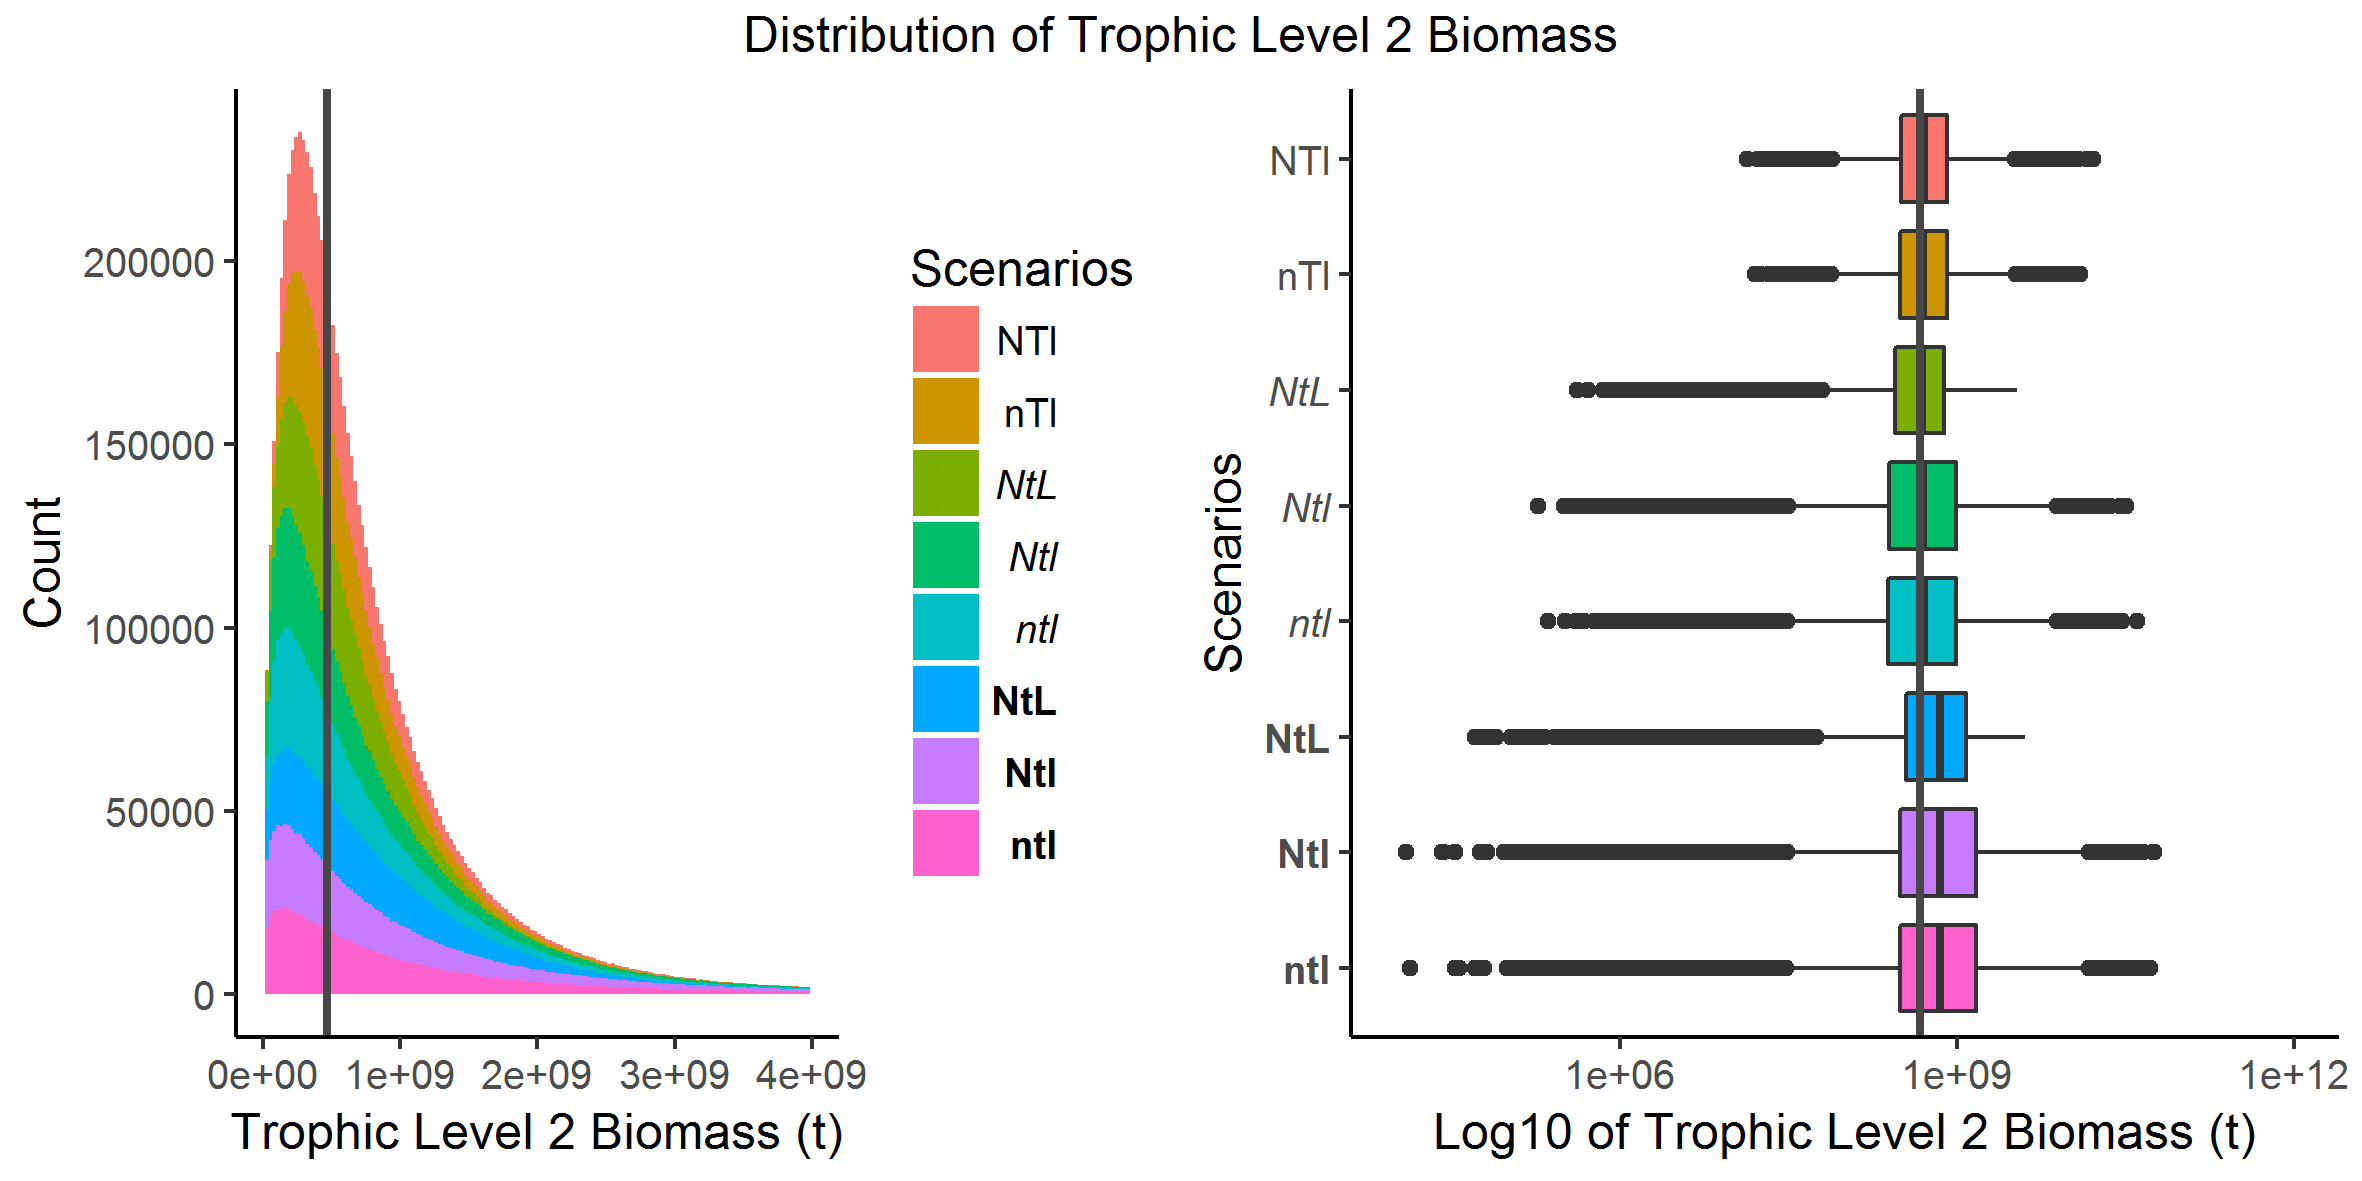
\includegraphics[width=1\textwidth]{fig/biomass2_hist_box_v3.png}
    \caption{Histogram and box plots of the trophic level 2 biomass ($\gamma_2$, metric tons) for all scenarios except Scenario NTL. Both plots have a vertical gray line representing the estimated trophic level biomass from Scenario NTL. Scenarios NTl and nTl show independent draws from analytical distributions, while the remaining scenarios show draws from simulations. In the histograms, we limited the upper bound of the x-axis to improve visualization. In the box plots, we addressed the skewness by plotting the log of the trophic level 2 biomass. The median of each distribution is denoted as a solid vertical black line inside each box. Plot created using R v.3.4.3 \cite{Rcite} ggplot2 package v.2.2.1 \cite{ggplot}. }
    \label{beta2estimated}
\end{figure}

% latex table generated in R 3.4.3 by xtable 1.8-2 package
% Fri Sep 28 15:23:56 2018
\begin{table}[ht]
\centering
\caption{Coefficient of variation for each trophic level biomass and scenario combination. Scenario 1 is not included because it is a deterministic equation.}
\begin{tabular}{cccc}
  \hline
 & Trophic level 2 & Trophic level 3 & Trophic level 4 \\ 
  \hline
  Scenario NTl & 0.79 & 1.00 & 0.97 \\ 
  Scenario nTl & 0.80 & 1.01 & 0.98 \\ 
  Scenario \textit{NtL} & 0.66 & 1.02 & 1.38 \\ 
  Scenario \textit{Ntl} & 1.15 & 1.77 & 2.16 \\ 
  Scenario \textit{ntl} & 1.16 & 1.77 & 2.17 \\ 
  Scenario \textbf{NtL} & 0.74 & 1.01 & 1.41 \\ 
  Scenario \textbf{Ntl} & 1.23 & 1.73 & 2.18 \\ 
  Scenario \textbf{ntl} & 1.24 & 1.76 & 2.20 \\ 
   \hline
\end{tabular}
\label{cv}
\end{table}

At the secondary consumer level ($h=3$), similar visual and mathematical patterns emerge at trophic level 3 that were found at trophic level 2. The distributions of trophic level biomass ($\gamma_3$) for all scenarios are right-skewed with heavy tails (Fig. \ref{beta3estimated}). The medians of Scenarios \textbf{NtL}, \textbf{Ntl}, and \textbf{ntl} are a bit larger than Scenario NTL's trophic level biomass estimate (Fig. \ref{beta3estimated}). The scenarios where transfer efficiency is a fixed 10\% between successive trophic levels (i.e., Scenarios NTl and nTl) and the scenarios where the maximum expected lifespan is kept as a fixed constant (i.e., Scenarios \textit{NtL} and \textbf{NtL}) have the smallest CVs. This is in contrast to the scenarios that allow the transfer efficiency to vary which have the largest CVs (Table \ref{cv}). In general when the transfer efficiency is treated as a random variable (i.e., Scenarios \textit{NtL}, \textit{Ntl}, \textit{ntl}, \textbf{NtL}, \textbf{Ntl}, and \textbf{ntl}), the variance and interquartile range increases. This is mostly attributed to the fact that these equations have more random values. Nevertheless, at trophic level 3 the dispersion has increased overall for all scenarios in comparison to the dispersion at trophic level 2. 

\begin{figure}[H]
     \centering
       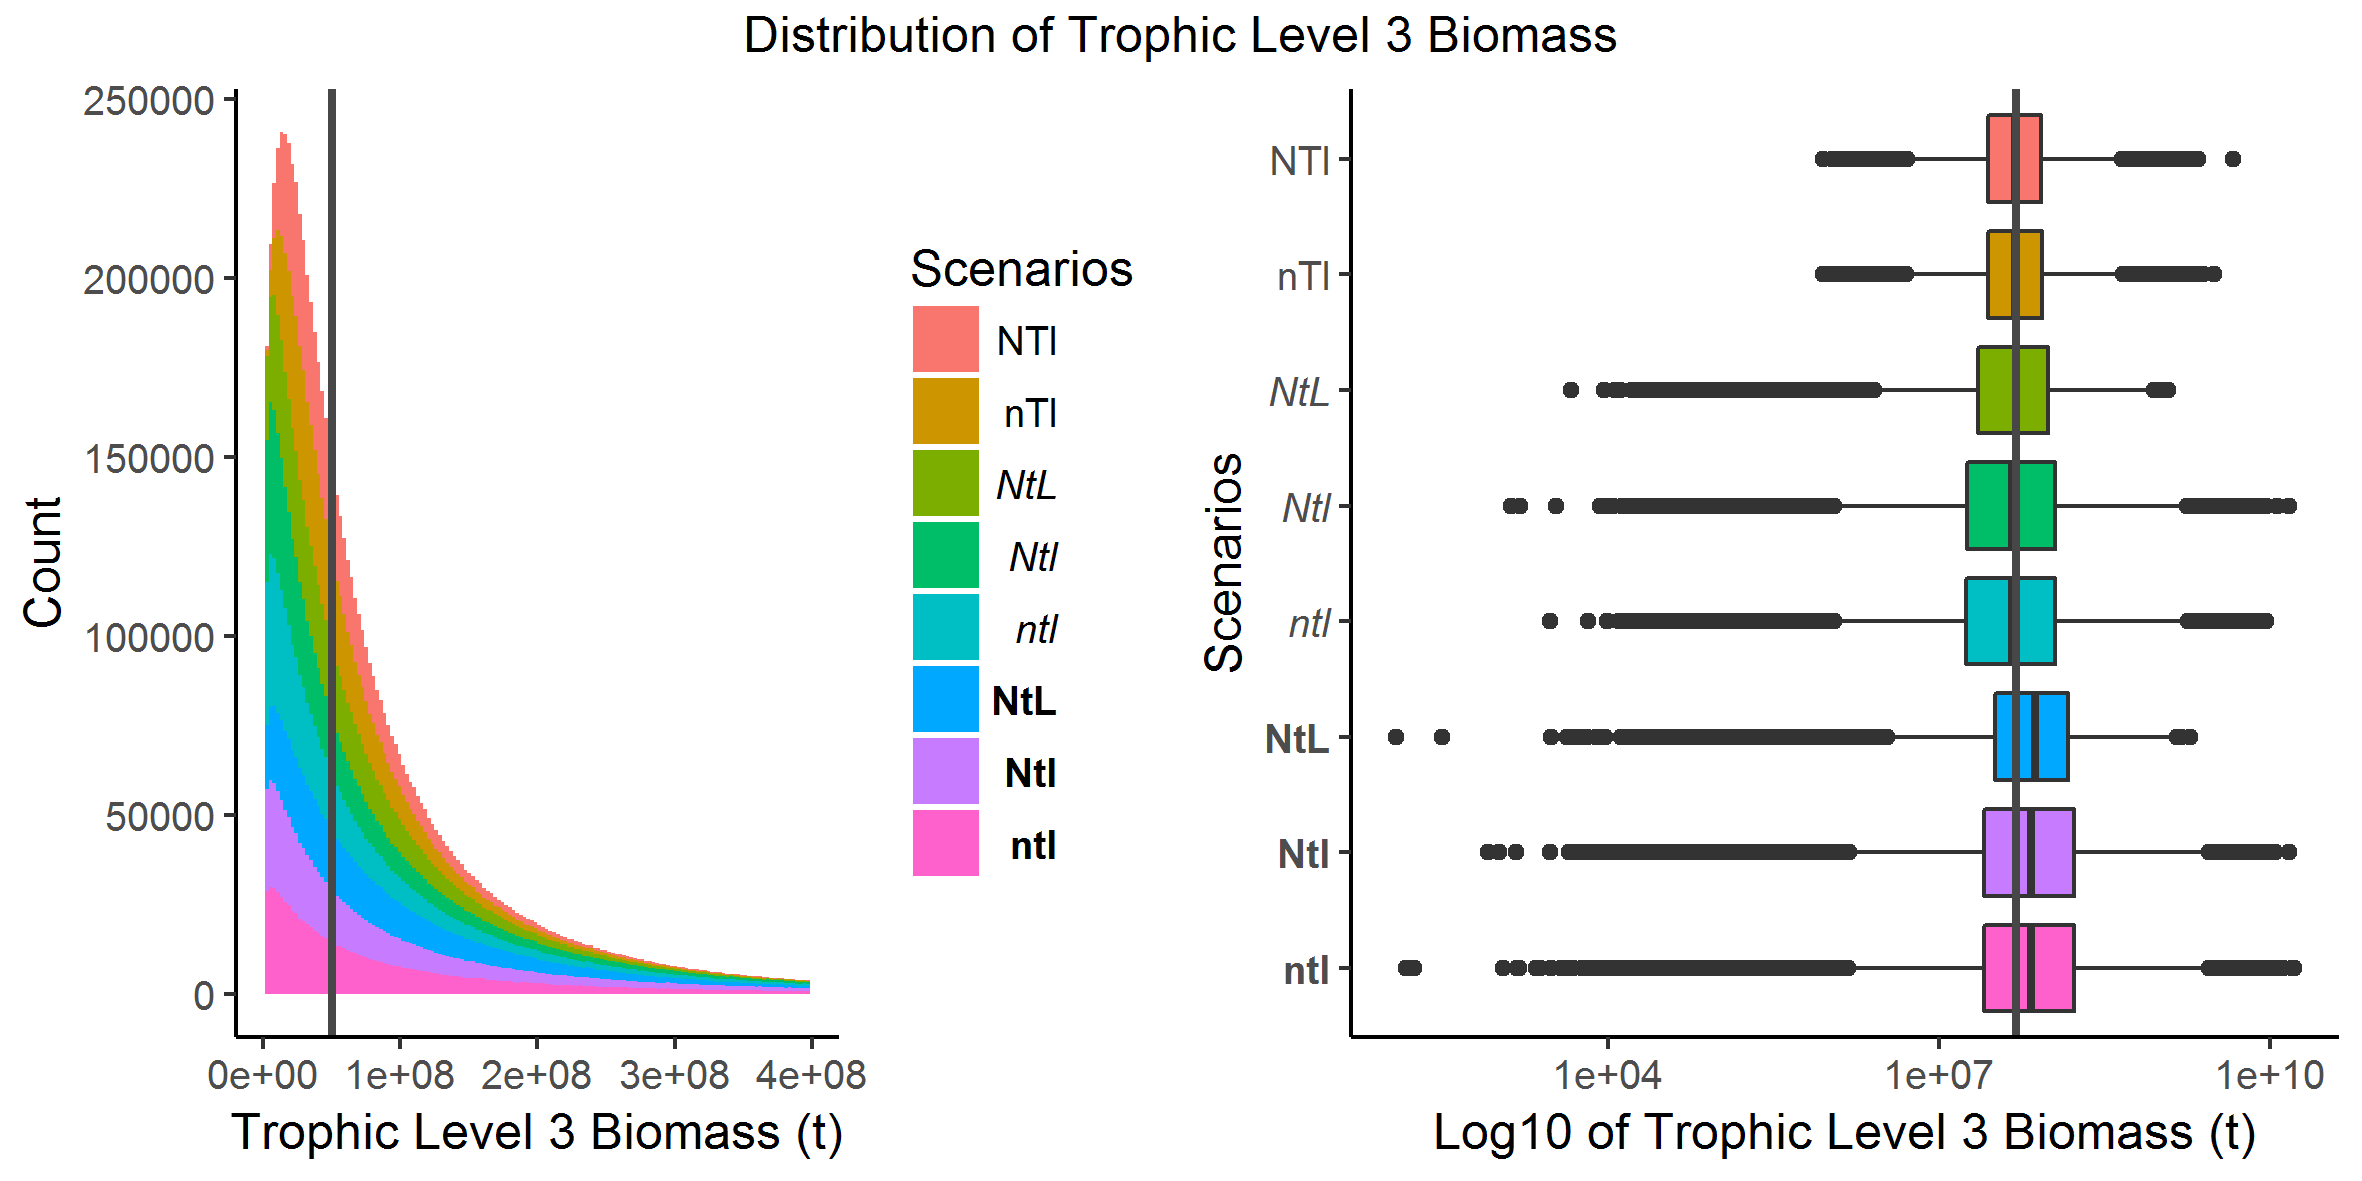
\includegraphics[width=1\textwidth]{fig/biomass3_hist_box_v3.png}
    \caption{Histogram and box plots of the trophic level 3 biomass ($\gamma_3$, metric tons) for except Scenario NTL. Both plots have a vertical gray line representing the estimated trophic level biomass from Scenario NTL. Scenarios NTl and nTl show independent draws from analytical distributions, while the remaining scenarios show draws from simulations. In the histograms, we limited the upper bound of the x-axis to improve visualization. In the box plots, we addressed the skewness by plotting the log of the trophic level 3 biomass. The median of each distribution is denoted as a solid vertical black line inside each box. Plot created using R v.3.4.3 \cite{Rcite} ggplot2 package v.2.2.1 \cite{ggplot}. }
    \label{beta3estimated}
\end{figure}

At the tertiary consumer level ($h=4$), most of the same distributional and dispersion patterns emerge at trophic level 4 that were found at the previous two trophic levels. The distributions of trophic level biomass ($\gamma_4$) for all scenarios are right-skewed with heavy tails (Fig. \ref{beta4estimated}). However at trophic level 4, the medians for all scenarios are relatively the same (Fig. \ref{beta4estimated}). Scenarios NTl and nTl, which both treat the transfer efficiency as a fixed 10\% constant, have the smallest interquartile ranges, but they have smaller CVs at trophic level 4 than at trophic level 3 (Table \ref{cv}). For the other scenarios though, the simulations show an increase in the CVs at trophic level 4 in comparison to the CVs at trophic level 3. 

\begin{figure}[H]
     \centering
       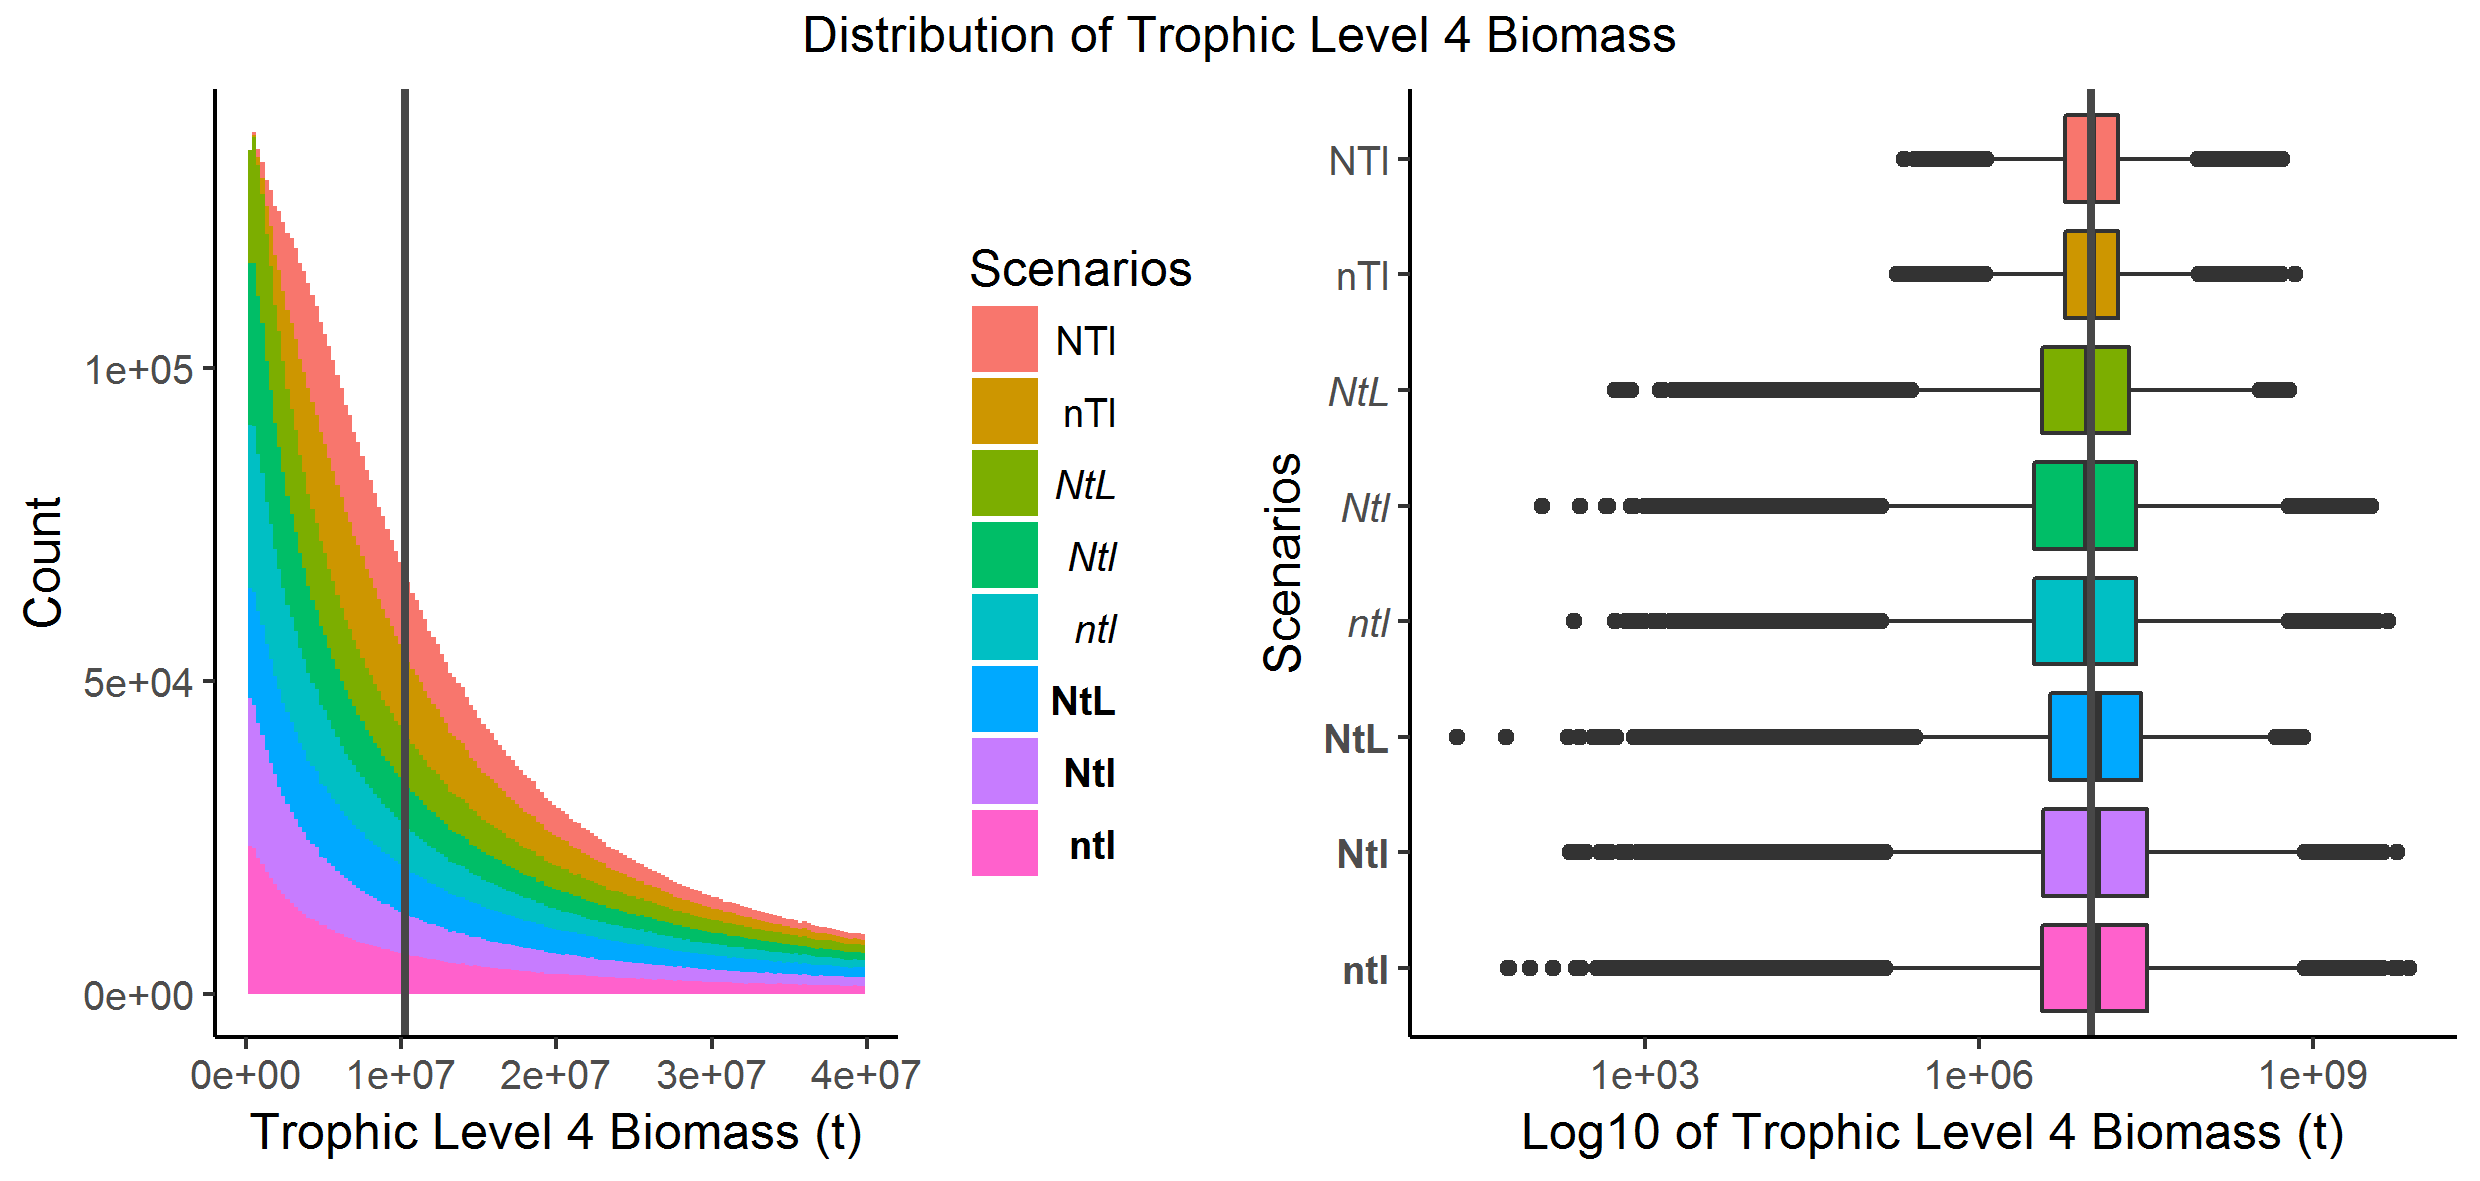
\includegraphics[width=\textwidth]{fig/biomass4_hist_box_v3.png}
    \caption{Histogram and box plots of the trophic level 4 biomass ($\gamma_4$, metric tons) for except Scenario NTL. Both plots have a vertical gray line representing the estimated trophic level biomass from Scenario NTL. Scenarios NTl and nTl show independent draws from analytical distributions, while the remaining scenarios show draws from simulations. In the histograms, we limited the upper bound of the x-axis to improve visualization. In the box plots, we addressed the skewness by plotting the log of the trophic level 4 biomass. The median of each distribution is denoted as a solid vertical black line inside each box. Plot created using R v.3.4.3 \cite{Rcite} ggplot2 package v.2.2.1 \cite{ggplot}. }
    \label{beta4estimated}
\end{figure}


\section*{Discussion}
Even though we placed different distributional assumptions on each of the scenarios, some common visual and mathematical patterns emerge in Fig. \ref{beta2estimated}, \ref{beta3estimated}, and \ref{beta4estimated} and in Table \ref{cv}. While the medians stayed relatively the same amongst the scenarios, the level of variability differed depending on the distributional assumptions. The simulations demonstrate that we can cluster the scenarios into 3 groups: fixed transfer efficiency (i.e., NTl and nTl), random transfer efficiency (i.e., \textit{NtL}, \textit{Ntl}, and \textit{ntl}), and decreasing transfer efficiency (i.e., \textbf{NtL}, \textbf{Ntl}, and \textbf{ntl}). These communal patterns indicate that the distributional assumptions placed on the transfer efficiency affects the distribution of trophic level biomasses more than the assumptions placed on NPP and maximum expected lifespan. Therefore by ignoring the variability in transfer efficiency, researchers will draw incorrect conclusions about biomass. 

\vspace{5mm} 

The results of the simulations provides direct insight on the MHI, which can in turn be used to inform management on the data-limited MHI Deep7 Bottomfish Complex groundfish fishery. This trophic pyramid food web model, which incorporates variability as an essential feature, now allows fisheries scientists to estimate trophic level biomasses with uncertainty assessment. Fisheries scientists now have a better idea of the biomasses that the MHI ecosystem can support, and they can utilize this information to help ground truth carrying capacity estimates for the groundfish fishery. Since the boxes in Fig. \ref{beta2estimated}, \ref{beta3estimated}, and \ref{beta4estimated} representing the various combinations of ecological assumptions mostly overlap, scientists can essentially choose any of them to estimate trophic level biomass in a data-limited case. However if this were a data-rich situation and fisheries scientists knew the ecological assumptions, they should choose the scenario that is most appropriate for their region.
 
\vspace{5mm} 

The results of the simulations demonstrate the need for incorporating variation in the modeling process, especially in data-limited cases. When we allowed the parameters (i.e., NPP, transfer efficiency, and maximum expected lifespan) in the trophic pyramid food web model to vary, we obtained a large range of potential trophic level biomasses from the simulations. We recommend that scientists use the scenarios that incorporate variation, because otherwise the model could potentially not encapsulate all potential biomass values. There is a higher probability that the true biomass of some species might fall above or below the estimated value if a single point estimate was used instead. Especially in data-limited cases, fisheries scientists should always model variability since little ecological and biological information is known about the system. Doing this can help avoid disastrous situations (e.g., population and fisheries collapse). From there, depending how conservative the fisheries management bodies are, fisheries scientists can advise catch limits where the catch cannot exceed the maximum estimated trophic level biomass or even half of that. If the goal is conservation, such as in places with multiple endangered species, managers can error on side of caution and pick lower bounds.

\vspace{5mm} 

Another reason scientists should want to incorporate variability is that the environment is not static. Even though it might appear on average to be acceptable to use a fixed NPP or transfer efficiency, there is year-to-year variability in everything from the input to the amount of energy that flows. It is well documented and understood that marine primary production changes seasonally and annually. Most notably within the past few decades, research has also examined how climate change has and will impact primary production \cite{gregg2003ocean} and species composition \cite{walther2002ecological}. Research also shows that transfer efficiency varies by ecological system, geographic location, trophic level, and species composition \cite{baird2004energy, barnes2010global, libralato2008novel, san2006latitudinal}. \citet{condon2011jellyfish} even found that the presence of jellyfish blooms, which have been increasing worldwide, have been found to restrict the transfer of energy to higher trophic levels. Therefore, we want models that are adjustable, especially in context of data-limited fisheries. Error bounds give a more realistic picture of what is happening in the system.

\vspace{5mm}

In addition, when summarizing data sets it is common practice to record only the mean and standard deviation of the given dataset. However, this proves problematic for other researchers needing to draw on data from multiple sources as these two summary statistics alone are insufficient to produce robust models. When choosing what to archive and make public, we argue that more information needs to be included in the databases (e.g., approximate distributions and parameter estimates). Knowing the specific distributions increases the accuracy of simulations, leading to more useful models.

\vspace{5mm}

Furthermore, we acknowledge that our NPP uncertainty estimate is underestimated due in part to the incomplete data set gathered by the SeaWiFS satellite. The satellite has missing information due to cloud cover, and the data set gathered has a shorter time series than the original time it was in operation due to parts malfunctioning. As a result, our model does not account for all of the NPP that is produced in the ocean. Additionally, the time series model (i.e., SARIMA) we used was simplistic. 
In future work on this topic, a more complicated time series approach will be utilized, as well as more specific estimates of NPP by season and by year.

\vspace{5mm}

The results of our simulations gives insight into the rigor of information we obtain when ecological concepts are incorporated into fisheries models and additionally how this information can be applied in fisheries assessments. Estimating trophic level biomass in data-limited scenarios is feasible, and our simulations yield a plausible range of biomass values. The multiple scenarios provide different options for tackling the same problem, and fisheries scientists can choose between them based on their knowledge of the system. The general ecosystem information provided from the results of the trophic pyramid food web model can help ground truth data-limited single-species estimates by giving an estimate of the biomass that the ecosystem can support. We therefore suggest using deterministic food web models results with caution and encourage future development on food web models to improve their usefulness in data-limited scenarios. 


%=== Chapter 3  ============================================
\chapter{Ecosystem knowledge in Bayesian surplus production models--what can it tell us?}
%---  Introduction -------------------------

\section*{Introduction}
Ecosystem models make use of different types of data than traditional stock assessment models and have the ability to describe a wide range of environmental states. While many ecosystem models do not provide the kind of results applicable to fisheries management, they may be available to provide new information to data-limited systems such as the biomass available at an ecosystem-level. For example in Chapter 3: Untangling uncertainty in food web models, the trophic pyramid food web model I developed cannot tell the commercial fishing operations exactly how much fish to catch, but the model can tell fisheries management what's a realistic carrying capacity for the ecosystem, which may be useful in determining catch limits at a larger scale. Other existing ecosystem models are complex and require similar data types that are used in traditional stock assessment models. Often, the data demands of these ecosystem models far exceed those of stock assessment models. We theorize that in some situations combining the simpler ecosystem models that use alternative data types with data-limited stock assessments may improve assessment reliability. 

\vspace{5mm}

Data-limited assessment models struggle due to lack of data. When species are aggregated and modeled as a complex in data-limited assessments, they are assumed to share similar life history traits. When this assumption is not met, we can obtain inaccurate predictions of biomass and set unsustainable levels of catch for some or all of the species in the complex. We hypothesize one way to provide more information in data-limited assessments is to use ecosystem models and link the data-limited assessment models with ecosystem models. 

\vspace{5mm}

Bayesian methods incorporate additional information in the form of prior distributions placed on some or all of the parameters \cite{mcallister1998bayesian}. The use of additional information has been used to combat data limitation issues, as many fish stocks often contain little information about the key parameters found in population dynamics models. In conventional approaches to stock assessment, uncertainties in the parameters are often ignored and point estimates or assumed values are used instead. However, values for such parameters may be similar among ecologically and taxonomically similar populations and could be incorporated into Bayesian stock assessment in the form of prior probability distributions, alleviating data limitations \cite{mcallister1998bayesian}. Using ecosystem information as prior information in the model may provide an alternative way of collecting estimates of some population dynamic parameters that can be incorporated directly in population dynamics models. Thus, the estimates of the parameters are constrained to more realistic values. 

\vspace{5mm}

In this study, we investigated the feasibility of incorporating ecosystem knowledge into existing single-species models, specifically for data-limited fisheries. We created two Bayesian models: a classic Bayesian surplus production model and a Bayesian surplus production model that includes ecological information. We then used a trophic pyramid food web model to estimate the distribution of trophic level biomasses. Finally, within a Bayesian framework, we linked that information with multiple single-species models’ carrying capacities. By combining these approaches, we determined if the indirect use of ecological information can help constrain the selection process for the carrying capacity of the ecosystem.  


\section*{Methods}
\subsection*{Case Study}
We selected a data-limited fishery in the main Hawaiian Islands (MHI) for our case study. The Hawaii bottomfish complex uses traditional deep handline capture methods for commercial and recreational harvest of the thirteen species of snappers, jacks, and groupers inhabiting the Hawaiian Archipelago. These species occupy different ecological niches, including both shallow- and deep-water habitats. A subset of the Hawaii bottomfish complex have similar life history traits and distributions (Table \ref{names}). These species have been clustered together into their own complex called the Hawaii Deep7 Bottomfish and have been the focus of fisheries management for the past few assessments (see \citealt{langseth2018stock}). However, limited information is known about their life history traits. Scientists assessing this fishery are concerned that life history traits (e.g., intrinsic growth rate, carrying capacity, etc.) vary drastically amongst the Deep7 Bottomfish complex, which could detrimentally impact the legitimacy of the projected biomass for one or all of the bottomfish species. Nonetheless, the last few published stock assessments used a single production model to determine the impacts of fishing for all seven species in the Hawaii Deep7 Bottomfish complex  \cite{brodziak2009hawaiian,langseth2018stock}. 

\begin{table}[H]
\centering
\caption{Common, Hawaiian, and Scientific names of the Hawaii Deep7 Bottomfish complex}
\begin{tabular}{lll}
  \hline \small
 Common name & Hawaiian Name & Scientific Name \\ 
   \hline
Sea bass & Hapuupuu & \textit{Hyporthodus quernus} \\
Snapper & Kalekale & \textit{Pristipomoides sieboldii} \\
Pink snapper & Opakapaka & \textit{Pristipomoides filamentosu}s \\
Squirrelfish snapper & Ehu & \textit{Etelis carbunculus} \\
Longtail snapper & Onaga & \textit{Etelis coruscans} \\
Silver jaw jobfish & Lehi & \textit{Aphareus rutilans} \\
Snapper & Gindai & \textit{Pristipomoides zonatus} \\
   \hline
\end{tabular} 
\label{names}
\end{table}

\subsection*{Data from the Main Hawaiian Islands Deep7 Bottomfish Complex Through 2010 Assessment}
\subsubsection*{Catch and CPUE Data}
We utilized fishery catch and standardized catch-per-unit-effort (CPUE) indices data from the stock assessment on the Main Hawaiian Islands Deep7 Bottomfish Complex Through 2010 \cite{langseth2018stock} in our analysis. The assessment reported species-specific total reported and unreported catch from 1949-2016 and aggregated CPUE data from 1948-2015. To keep a consistent time line, we only used catch and CPUE data that fell between 1949-2015 (Fig. \ref{catchandcpue}).

\begin{figure}[H]
     \centering
       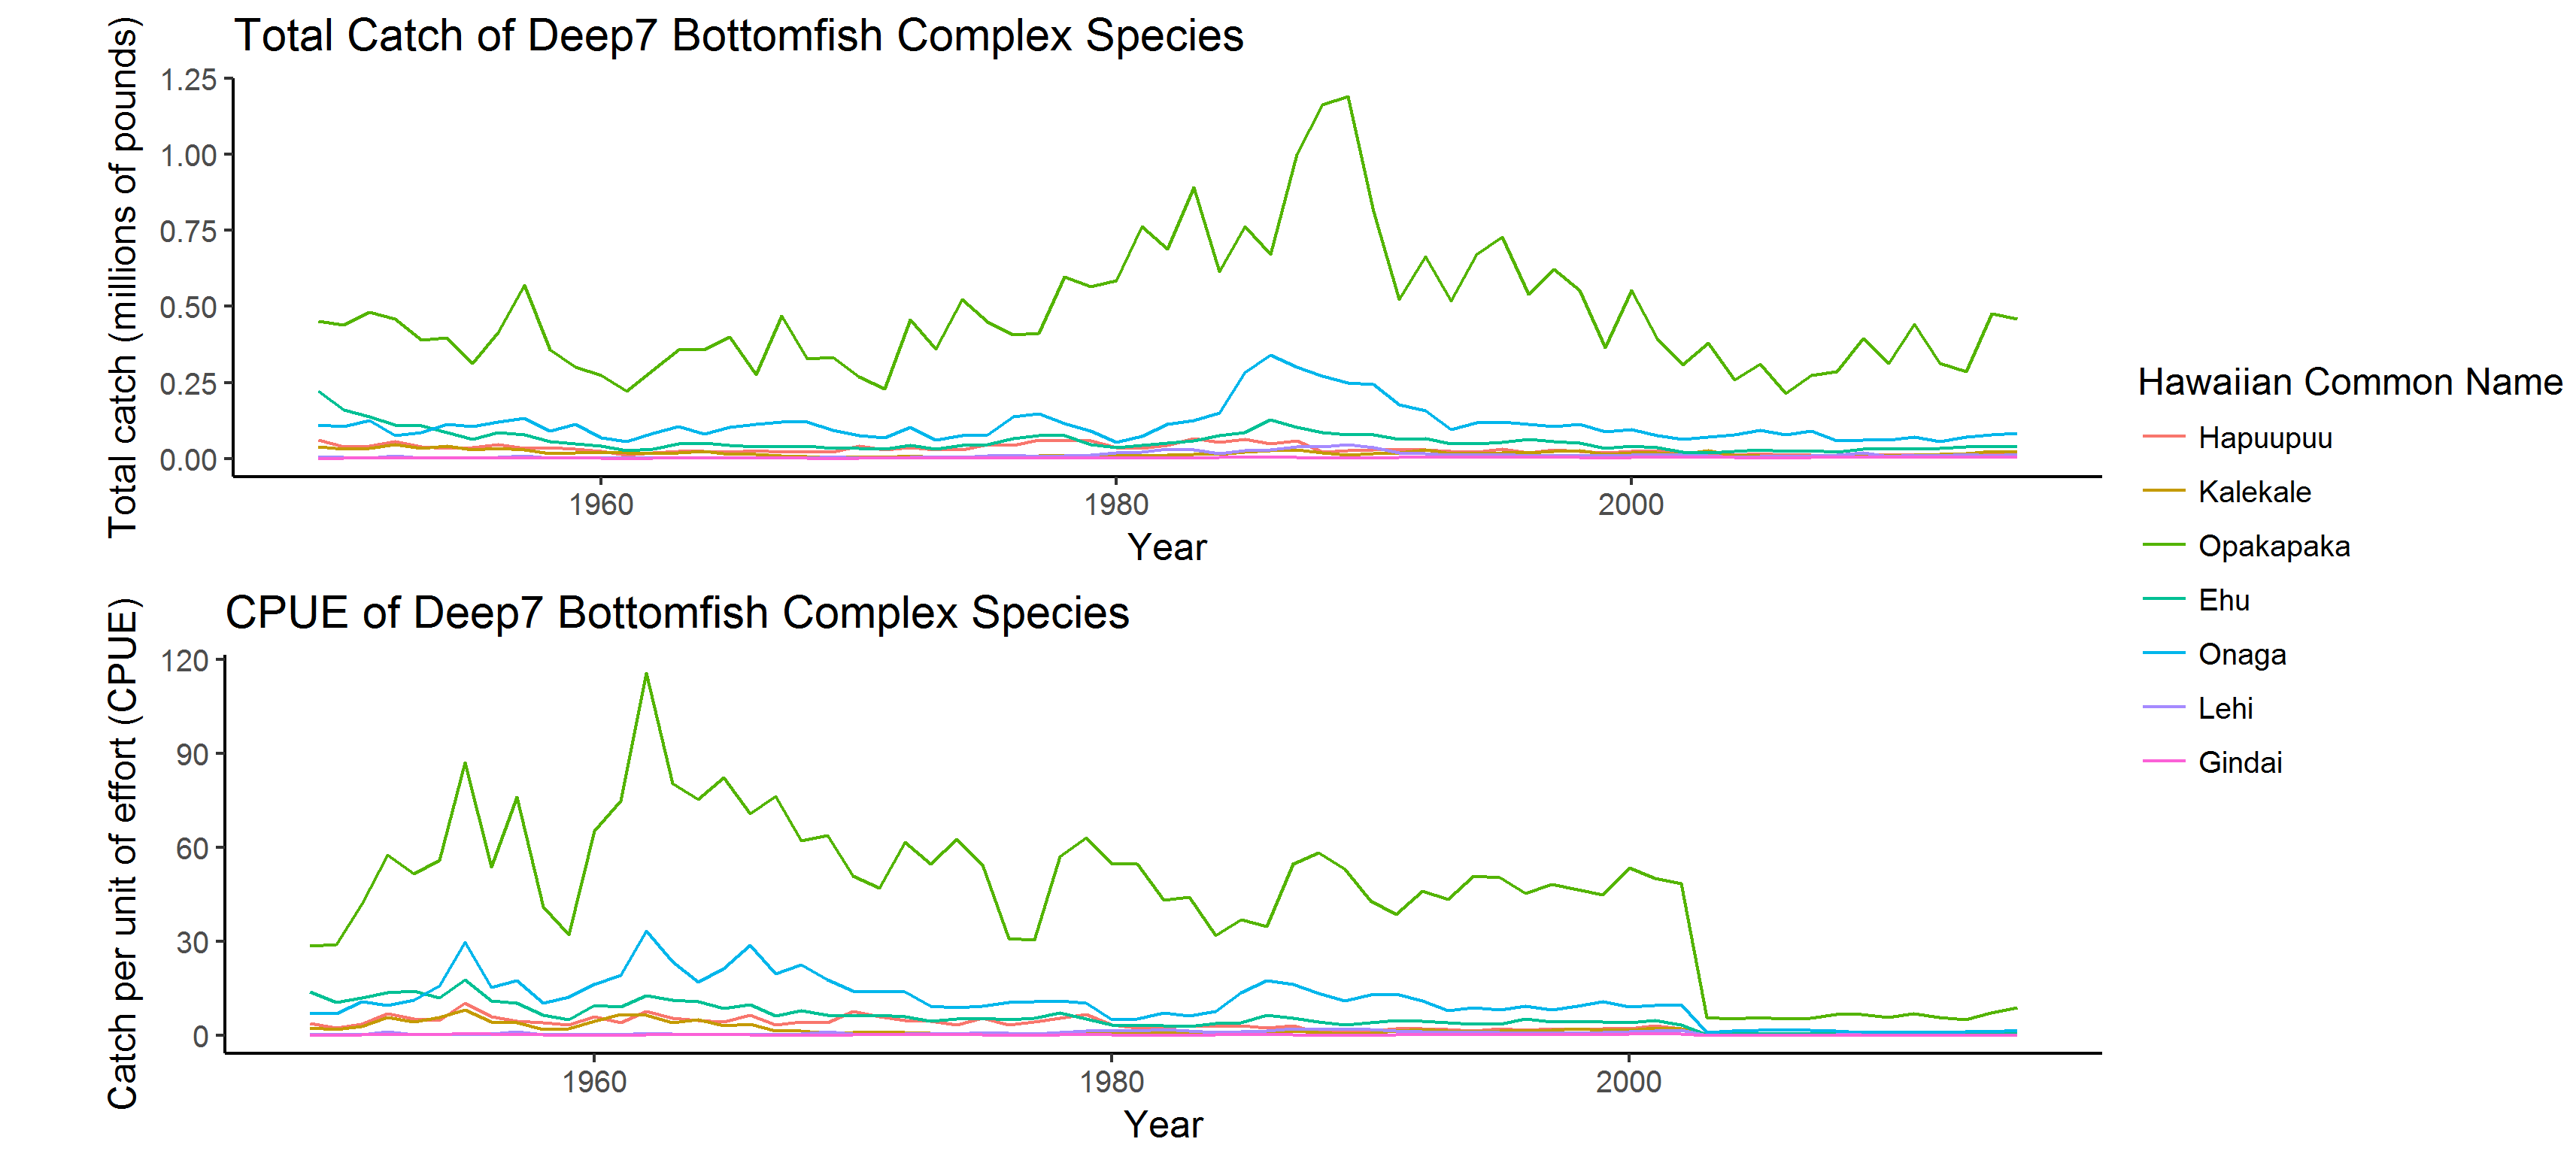
\includegraphics[width=\textwidth]{fig/catch_cpue}
    \caption{Time series of total catch and CPUE for the Seven Bottomfish Species in the Deep7 Bottomfish Complex. Plot created using R v.3.4.3 \cite{Rcite} ggplot2 package v.2.2.1 \cite{ggplot}. }
    \label{catchandcpue}
\end{figure}

In order to obtain species-specific estimates of CPUE per year ($CPUE_{i,t}$) from the aggregated CPUE data ($CPUE_t^*$) from \cite{langseth2018stock}, we assumed that catch in year $t$ for species $i$ is proportional to abundance (Eq. \ref{proportion}). In Eq. \ref{proportion}, $C_{i,t}$ refers to catch of species $i$ in year $t$ for species $i$ where $i=1,\dots,n$. We assume independence across years. We took the proportion outlined in Eq. \ref{proportion} to scale the aggregated CPUE data and obtain species-specific estimates of CPUE per year (i.e., $CPUE_{i,t}$) (Fig. \ref{catchandcpue}).

\begin{equation} \label{proportion}
CPUE_{i,t} = \frac{C_{i,t}}{\sum_{i=1}^{n}C_{i,t}}*CPUE_t^*
\end{equation}

\subsection*{Logistic Surplus Production Models}
We fitted logistic (Schaefer) surplus production models with relative abundance indices as our biomass dynamics models (Eq. \ref{production}) \cite{schaefer1954some}. In Eq. \ref{production}, for species $i$ where $i=1,\dots,n$ a population's biomass in year $t$ ($B_{i,t}$) is dependent on the previous year's biomass ($B_{i,t-1}$), the species' intrinsic growth rate ($r_i$), the population's carrying capacity ($K_i$), and the previous year's fishery catch ($C_{i,t-1}$). To clarify, $B_{i,t}$ represents a matrix with dimension $i\times t$, whereas $K_i$ is a vector with dimension $i$. We assume that $r_i=r_j \hspace{2mm} \forall \hspace{2mm} i,j$. All $r_i$ are identical. Thus for the sake of brevity, we will refer to it simply as $r$. However, each value of $K_i$ is unique for species $i$. We also assume independence across years. In year zero (i.e., 1949), we set the estimated biomass equal to the virgin unfished biomass $K_i$. The two parameters that require estimation in Eq. (\ref{production}) are $r$, where $r$ is defined between 0 and 1 and $K_i$, where $K_i > 0$. See Table \ref{production_table} for defined variables and parameters definitions within Eq. (\ref{production}).

\begin{equation} \label{production}
B_{i,t} = B_{i,t-1} + r*B_{i,t-1} \left(1- \frac{B_{i,t-1}}{K_i} \right)-C_{i,t-1} 
\end{equation}

\begin{table}[H]
\centering
\caption{Definition of notation in Eq. (\ref{production}) and scientific units used}
\begin{tabular}{l|l|l}
  \hline \small
 Terms & Description & Units  \\ 
   \hline
   \multirow{2}{*}{$B_{i,t}$} & Predicted biomass in year $t$ where $t$ $\in \{1949,\dots,2015\}$  & \multirow{2}{*}{millions of lbs} \\
     &  for species $i$ where $i=1,\dots,n$  &   \\      
   $B_{i,t-1}$ &  Predicted biomass in year $t-1$ for species $i$ & millions of lbs  \\
   $r$ & Intrinsic growth rate for species & \\
   $K_i$ & Carrying capacity for species $i$ & millions of lbs  \\  
   $C_{i,t-1}$ & Total fishery catch of species $i$ in year $t-1$ & millions of lbs \\
   \hline
\end{tabular} 
\label{production_table}
\end{table}

\subsubsection*{Catch per Unit Effort (CPUE)}
We define catch per unit effort ($CPUE_{i,t}$) as the total weight in pounds for species $i$ in year $t$ caught divided up the unit of effort in year $t$ (Eq. \ref{cpue}). Effort is defined in \citet{langseth2018stock} as the number of days fishing prior to October 2002 and the number of hours fishing since October 2002. Catch is recorded daily. Both catch and effort are aggregated to obtain yearly estimates. Effort is assumed to be the same for all species $i$. We assume independence across years. Table \ref{cpue_table} describes notation and units for Eq. \ref{cpue}.

\begin{equation} \label{cpue}
CPUE_{i,t} = C_{i,t}/E_t 
\end{equation}

\begin{table}[H]
\centering
\caption{Definition of notation in Eq. (\ref{cpue}) and scientific units used}
\begin{tabular}{l|l|l}
  \hline \small
 Terms & Description & Units  \\ 
   \hline     
   $CPUE_{i,t}$ & Catch per unit of effort in year $t$ for species $i$ & millions of lbs/time spent fishing \\
   $C_{i,t}$ & Total fishery catch of species $i$ in year $t$ & millions of lbs \\
   $E_t$ & Effort in year $t$ & time spent fishing \\
   \hline
\end{tabular} 
\label{cpue_table}
\end{table}

\subsubsection*{Catchability}
Catchability is defined as the fish caught per fish available per unit of effort and per time unit. The catchability coefficient is represented as $q_{i,t}$ for species $i$ at time $t$ in Eq. \ref{catchability}. We assume independence across years. 

\begin{equation} \label{catchability}
q_{i,t} = CPUE_{i,t}/B_{i,t}
\end{equation}

We can calculate an estimate of catchability coefficient $\widehat{q_{i}}$ using the equation below, where data is available on the total catch per species $i$ in year $t$ ($C_{i,t}$) and the observed relative abundance indices (i.e., $CPUE_{i,t}$) for species $i$ in year $t$ for years $1949-2015$. We let the total number of years in our dataset be represented as $m$. 

\begin{align*}
q_{i,t} &= CPUE_{i,t}/B_{i,t}  = CPUE_{i,t}/\left(B_{i,t-1} + r_i*B_{i,t-1} \left( 1- \frac{B_{i,t-1}}{K_i} \right)-C_{i,t-1} \right) \\
\widehat{q_{i}} &= e^{\frac{\sum_{t=1949}^{2015} ln(q_{i,t})}{m}}  \\
\end{align*}

\subsubsection*{Regression methods}
Using the relationship between Eq. \ref{production} and \ref{catchability}, we can substitute the predicted biomass $B_{i,t}$ in Eq. \ref{production} with $B_{i,t}=\frac{CPUE_{i,t}}{q_i} $. We outline the theory below discussed in \citet{hilborn1992quantitative} and use their assumption that the catchability coefficient $q_{i,t}$ is time invariant. Thus, we will refer to it as $q_i$.

\begin{align*}
B_{i,t} &= B_{i,t-1} + r*B_{i,t-1} \left(1- \frac{B_{i,t-1}}{K_i} \right)-C_{i,t-1} \\
\frac{CPUE_{i,t}}{q_i} &= \frac{CPUE_{i,t-1}}{q_i}  + r*\frac{CPUE_{i,t-1}}{q_i} \left(1-\frac{CPUE_{i,t-1}}{q_i}*\frac{1}{K_i} \right) - CPUE_{i,t-1}*E_{t-1} \\
CPUE_{i,t} &= CPUE_{i,t-1} + r*CPUE_{i,t-1} \left(1-\frac{CPUE_{i,t-1}}{q_i*K_i} \right) - CPUE_{i,t-1}*q_i*E_{t-1} \\
CPUE_{i,t} &= CPUE_{i,t-1} + r*CPUE_{i,t-1} -\frac{r*CPUE_{i,t-1}^2}{q_i*K_i}  - CPUE_{i,t-1}*q_i*E_{t-1} \\
CPUE_{i,t} &= CPUE_{i,t-1} \left(1 + r -\frac{r*CPUE_{i,t-1}}{q_i*K_i}  - q_i*E_{t-1} \right) \\
\frac{CPUE_{i,t}}{CPUE_{i,t-1} } &= 1 + r -\frac{r*CPUE_{i,t-1}}{q_i*K_i}  - q_i*E_{t-1} \\
\frac{CPUE_{i,t}}{CPUE_{i,t-1} } -1 &= r -\frac{r}{q_i*K_i}*CPUE_{i,t-1}  - q_i*E_{t-1} 
\end{align*}

Thus in the linear equation (Eq. \ref{regression}), $\frac{CPUE_{i,t}}{CPUE_{i,t-1} } -1$ is the dependent variable, the independent variables are $CPUE_{i,t-1} $ and $E_{t-1} $, and the parameters are $r, -\frac{r}{q_i*K_i},$ and $-q$ where $r$ is the intercept and $-\frac{r}{q_i*K_i}$ and $-q$ are the slopes. \citet{hilborn1992quantitative} noted however that this method does not always provide reliable parameter estimates and is biased. Thus, including prior information on the parameters can improve their estimation.

\begin{equation} \label{regression}
\frac{CPUE_{i,t}}{CPUE_{i,t-1} } -1 = r -\frac{r}{q_i*K_i}*CPUE_{i,t-1}  - q_i*E_{t-1} 
\end{equation}

\subsubsection*{Optimization} 
\citet{walters_fisheries_2004} explain that although in linear regression we assume the error structure follows a Normal distribution, ``we use the log-normal form because most quantitative observations in fish dynamics arise as a product of component and proportional observation/collect processes, and the sum of the logs of such proportions is likely to be normally distributed because of Central Limit Theorem effects." Therefore, we assume the log of the error structure follows a $Normal(0,\sigma_i^2)$ and used the maximum likelihood estimates (MLE) for $\sigma_i^2$.  

 \begin{align*}
SS_{i,t} & = ln(\widehat{q_{i,t}}*B_{i,t}) - ln(CPUE_{i,t}) \\
SSQ_i & = \sum_{t=1949}^{2015}[ln(\widehat{q_{i,t}}*B_{i,t}) - ln(CPUE_{i,t})]^2  \\
\widehat{\sigma_i} &=\sqrt{SSQ_i/m} \\
\end{align*} 

We then plugged in the value of zero for $\mu$ and the MLE estimate of $\widehat{\sigma_i^2}$ into the Normal probability distribution function (PDF) and solved for the negative log likelihood. 

\begin{align*}
L(\mu_i,\sigma_i^2) &= \prod_{t=1949}^{2015} \frac{1}{\sqrt{2\pi\widehat{\sigma_i}^2}}e^{-\frac{SS_{i,t}^2}{2\widehat{\sigma_i}^2}} \\
logL(\mu_i,\sigma_i^2) &= - \sum_{t=1949}^{2015} -(m/2)*ln(2\pi) - (m/2)*ln(\widehat{\sigma_i}^2) - \frac{SS_{i,t}^2}{2\widehat{\sigma_i}^2}
\end{align*}

The optimal values of $r$ and $K_i$ for species $i$ minimizes the log likelihood. We used the limited-memory modification of the Broyden, Fletcher, Goldfarb and Shanno quasi-Newton method for optimization \cite{shanno1970conditioning,byrd1995limited}. This method allows box constraints meaning the parameters being optimized (i.e., $r$ and $K_i$) can be given lower and/or upper bounds. 

\subsection*{Bayesian model}
We set up two Bayesian frameworks in our analysis: a classic Bayesian surplus production model and a Bayesian surplus production model that incorporates ecological information. The Bayesian surplus production models were applied on the individual populations and not the aggregated fishery complex. The posterior distribution for both cases are as follows:
 
\begin{align*}
\pi(\theta_i|y_i) & \propto \pi(\theta_i)L(\theta_i|y_i) \\
& \propto \pi(r)\pi(K_i)L(r,K_i|\hat{q_{i,t}}(r,K_i))
\end{align*}

The posterior distribution $\pi(\theta_i|y_i)$ is proportional to the prior information $\pi(\theta_i)$ and the sampling information $L(\theta_i|y_i)$. $\theta_i$ for species $i$ where $i=1,\dots,n$ can be partitioned as $\theta_i=(r,K_i,q_{i,t})$ where $r$ and $K_i$ are the parameters of interest and $q_{i,t}$ is the nuisance parameter. We place prior information on the intrinsic growth rate ($r$) and carrying capacity ($K_i$). Data $y_i$ can be partitioned into the total catch per species $i$ in year $t$ (i.e., $C_{i,t}$) and the observed relative abundance indices (i.e., $CPUE_{i,t}$) for species $i$ in year $t$ for years $t=1949-2015$. 

\vspace{5mm}

In both of the Bayesian frameworks, we ran 10,000 Monte Carlo simulations per species with the sampling/importance resampling algorithm (SIR) algorithm. Monte Carlo simulations with the SIR algorithm are a simple and versatile method for drawing a sample approximately from a target distribution \cite{mcallister1997bayesian, givens2012computational}. We based our approach off of the methods described in \citet{mcallister1997bayesian}. Samples from the posterior distribution of the production model parameters were simulated in order to make inferences.

\subsection*{Prior Information}
We place prior information from \citet{langseth2018stock} on the intrinsic growth rate ($r$) and carrying capacity ($K_i$) for species $i$ where $i=1,\dots,n$. In \citet{langseth2018stock}, the intrinsic growth rate ($r$) and carrying capacity ($K^*$) parameters are found to follow Lognormal distributions with mean values (0.11 and 27.55) and standard deviation (0.028 and 9.69) for $r$ and $K^*$ respectively.
We used the mean and variance equations of a Lognormal distribution to calculate the  values of the parameters for the Lognormal distribution. We assume $r$ and $K_i$ for species $i$ where $i=1,\dots,n$ are independent. While the prior information from \citet{langseth2018stock} for the intrinsic growth rate ($r$) could be applied to individual production models, the prior distribution for the carrying capacity ($K^*$) needed to be adjusted since it represents the carrying capacity estimate for the sum of the seven groundfish species. Figure \ref{priorr} visualizes the distribution of random draws from the prior distribution on the intrinsic growth rate $r$.

\begin{figure}[H]
     \centering
       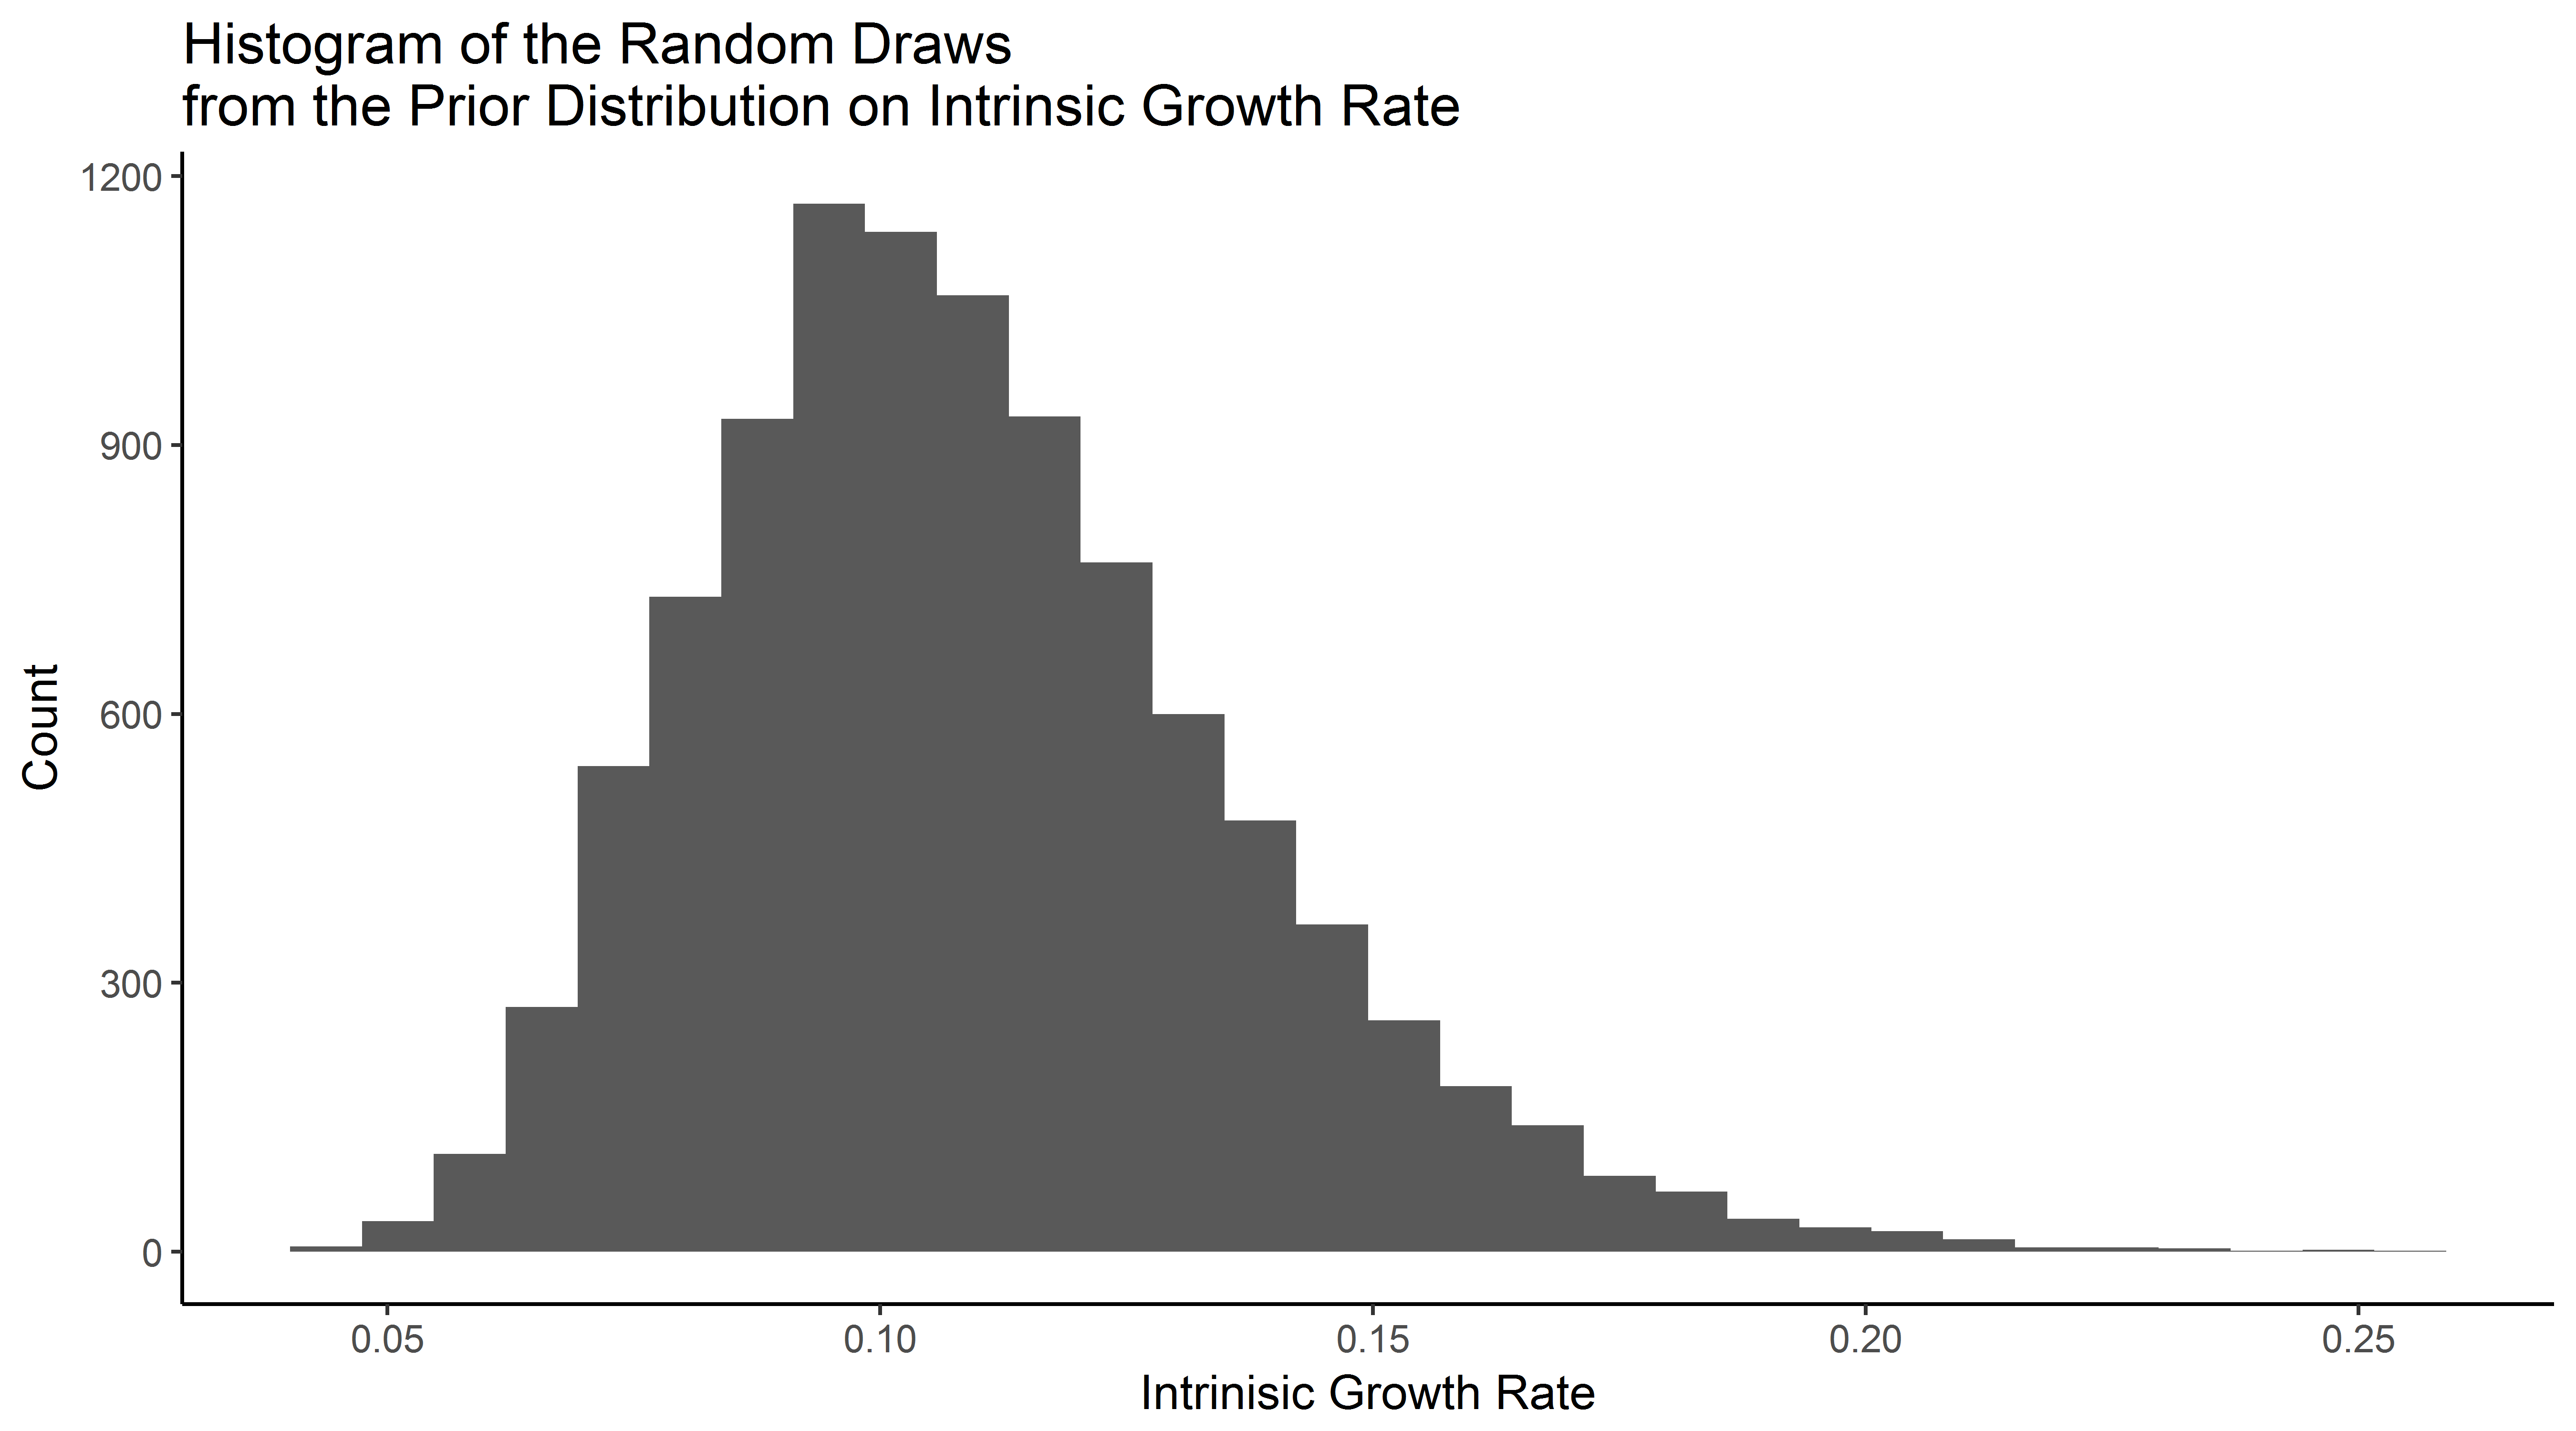
\includegraphics[width=.9\textwidth]{fig/hist_prior_r}
    \caption{Histogram of random values that come from the prior distribution on the intrinsic growth rate $r$. Plot created using R v.3.4.3 \cite{Rcite} ggplot2 package v.2.2.1 \cite{ggplot}. }
    \label{priorr}
\end{figure}

In order to put a prior distribution on the carrying capacities for each of the species, we created a hierarchical framework using hyperparameters and hyperpriors. We let the individual carrying capacities $K_1,...,K_n$ for species $i$ where $i=1,\dots,n$ come from a Multinomial distribution. We placed prior information on the parameters $N$ and $\boldsymbol{\delta}$. We let the distribution of the aggregate carrying capacity ($K^*$) be the hyperprior for the number of trials parameter ($N$) in the Multinomial distribution. We used our assumption that catch $C_{i,t}$ was proportional to abundance and calculated the average proportion of abundance for all  species to parameterize a Dirichlet distribution proportion parameter $\boldsymbol{\alpha}$. We define the total number of years as $m$.

\begin{equation*}
\boldsymbol{\alpha} = \frac{\sum_{t=1949}^{2015}\frac{C_{i,t}}{\sum_{i=1}^{n}C_{i,t}}}{m}
\end{equation*}

We then multiplied the random values from the Dirichlet distribution $\boldsymbol{\delta}$ by the average carrying capacity (i.e., 27.55 million lbs) and set $\boldsymbol{\delta}$ as the hyperparameter values for the proportion parameters in the Multinomial distribution. Figure \ref{priorK} visualizes the prior distribution of the carrying capacity $K_i$ for species $i=1,\dots,n$.

\begin{align*}
r & \sim Lognormal(\mu_r, \sigma_r^2) \\
K_1,\dots,K_n & \sim Multinomial(N=K^*, \boldsymbol{\delta}*2.755e+7) \\
K^* & \sim Lognormal(\mu_{K^*}, \sigma_{K^*}^2) \\
\boldsymbol{\delta} & \sim Dirichlet(\boldsymbol{\alpha})
\end{align*}

\begin{figure}[H]
     \centering
       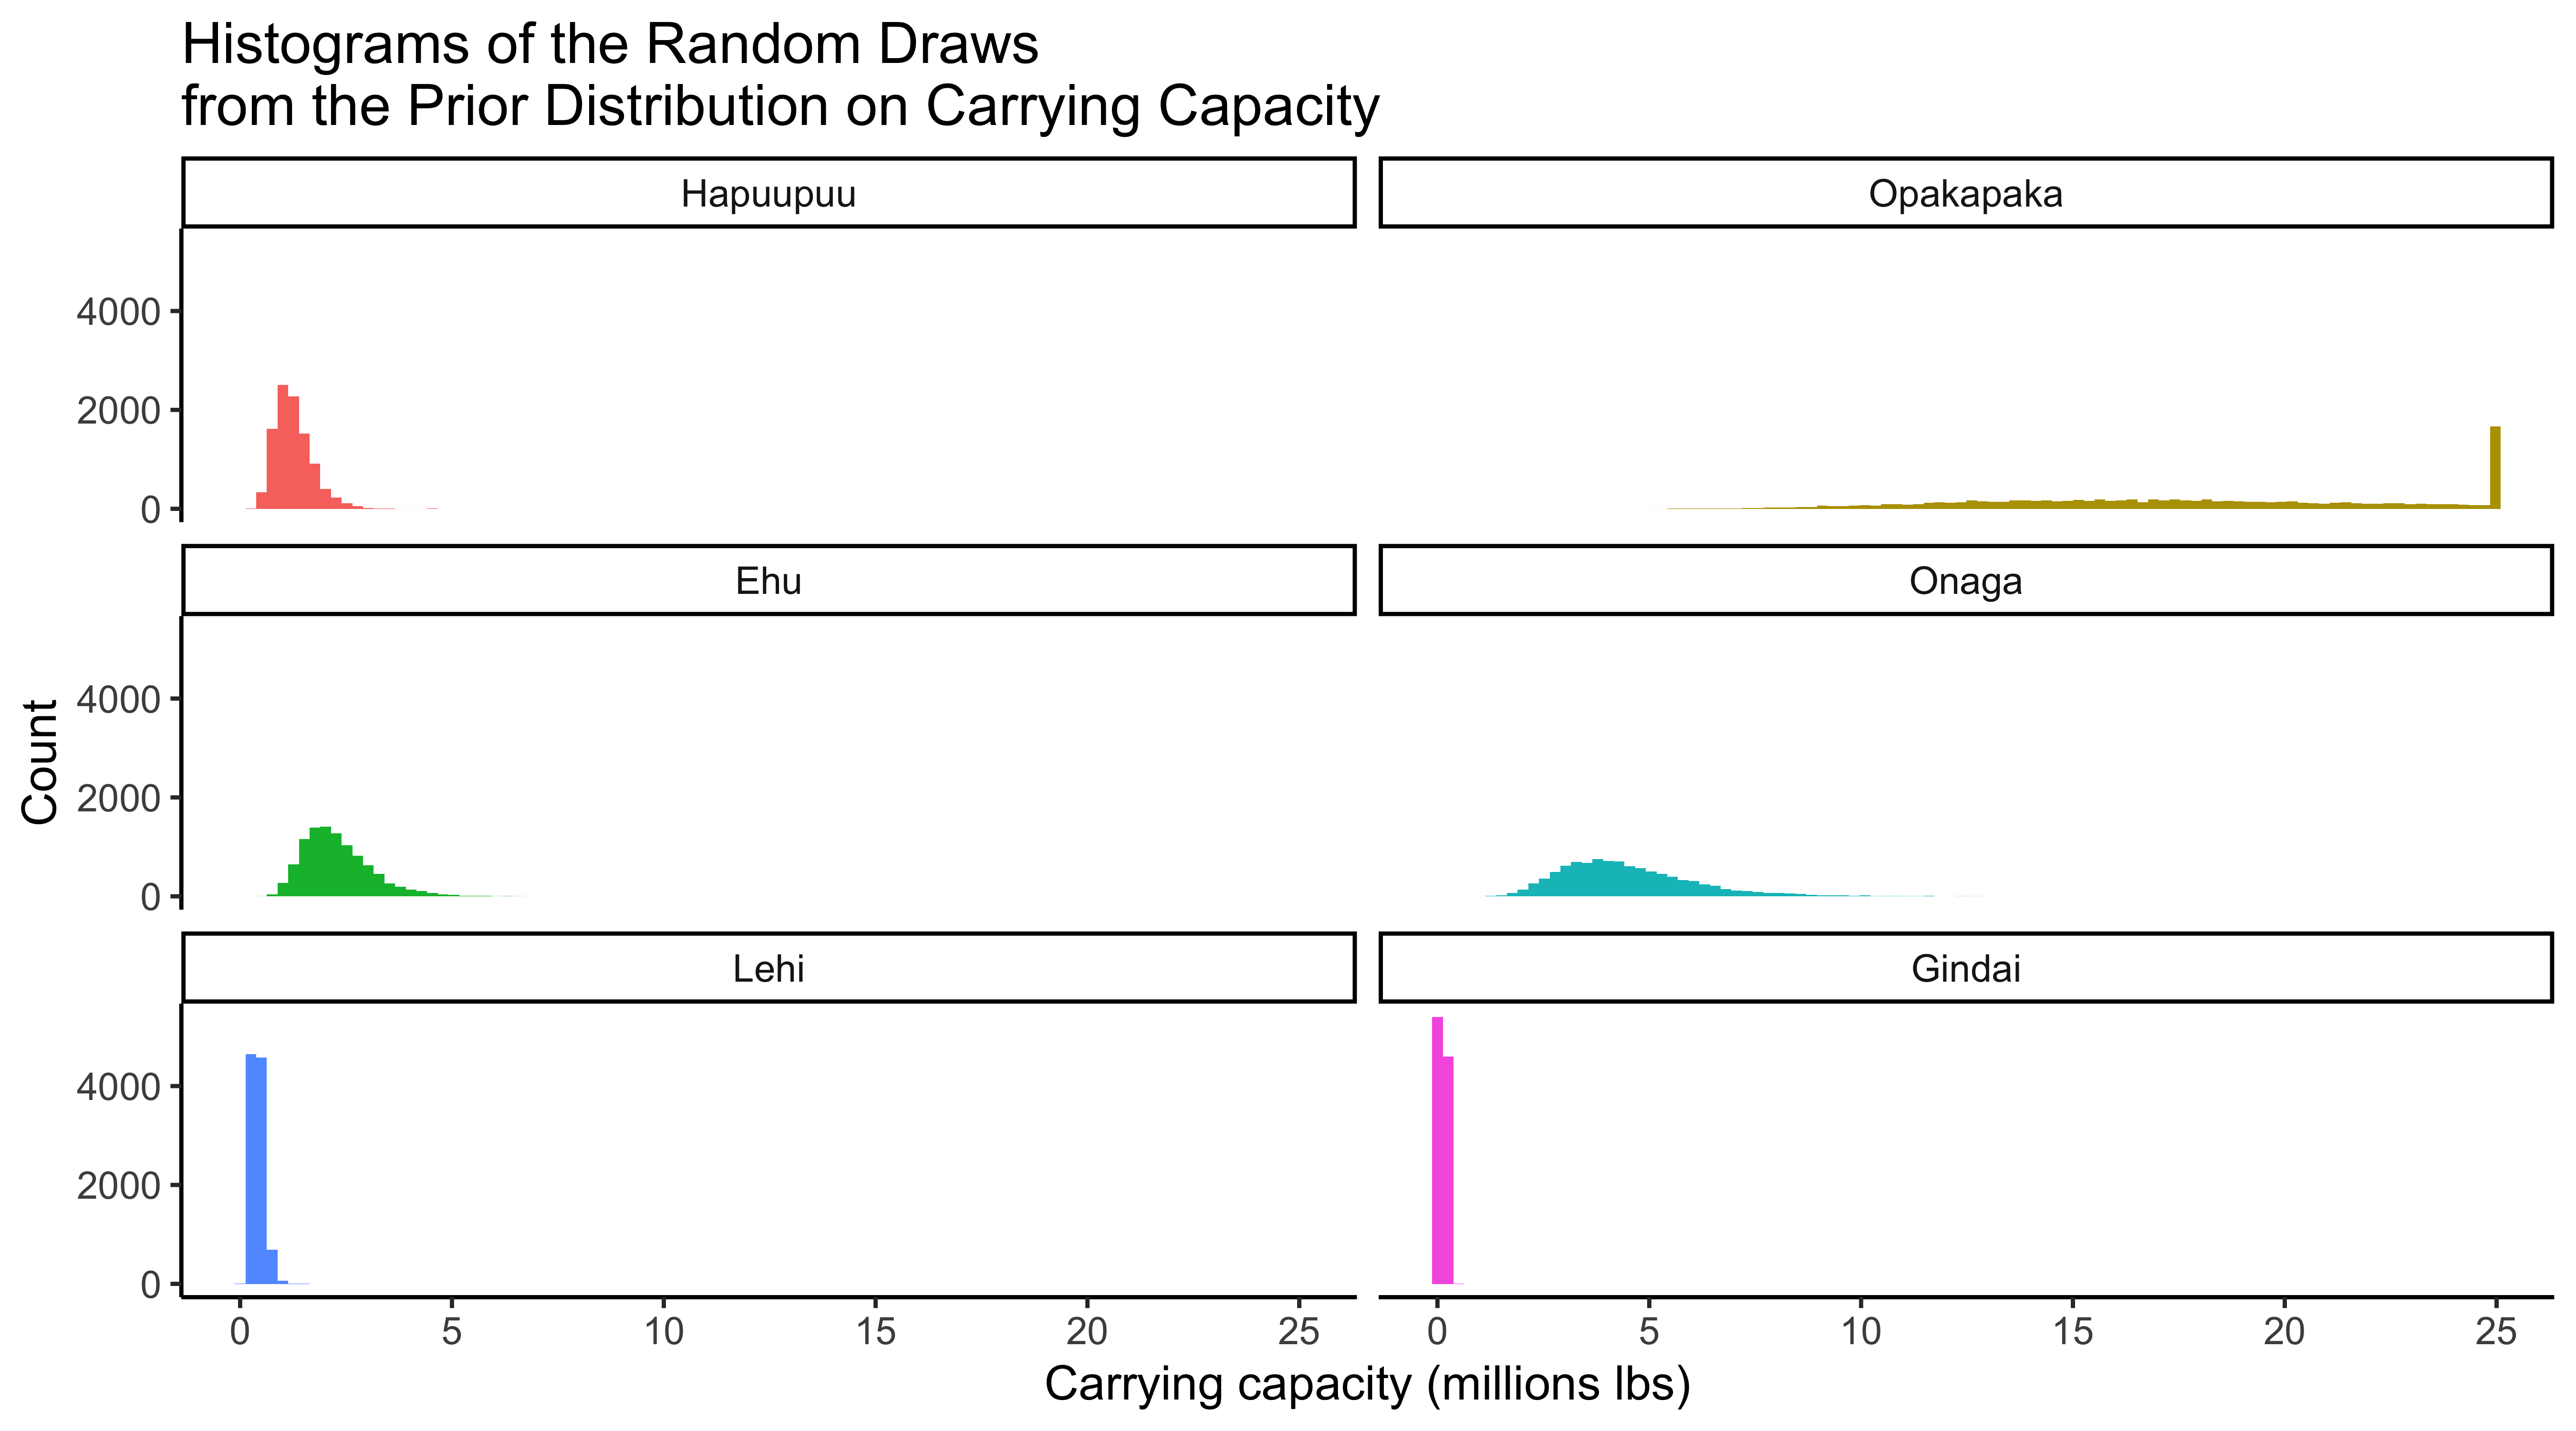
\includegraphics[width=.9\textwidth]{fig/hist_prior_K}
    \caption{Histogram of random values that come from the prior distribution on the carrying capacity $K_i$ for species $i=1,\dots,7$. We adjusted the far right bin width due to rare events. The original range extends out further. Plot created using R v.3.4.3 \cite{Rcite} ggplot2 package v.2.2.1 \cite{ggplot}.}
    \label{priorK}
\end{figure}

\subsubsection*{Bayesian Surplus Production Model}
Before fitting individual logistic (Schaefer) surplus production models, we clustered the bottomfish species by trophic level. We used the Fishbase database (\url{http://www.fishbase.org/}) of \citet{fishbase} to obtain information on trophic level. Out of the seven species, only Kalekale (\textit{Pristipomoides sieboldii}) occupies the third trophic level, with the remaining six occupying trophic level four. Therefore, we focused only the six species that occupied trophic level four since our main interest in this study was to test if the carrying capacity parameter could be constrained by ecological data. 

\vspace{5mm}

Thus, the current set of Bayesian models consisted of individual Bayesian surplus production models for the six species found at trophic level four. We set the values for the parameters to the fixed values described below for the prior distributions.

\begin{align*}
r & \sim Lognormal(\mu_r = -2.24, \sigma_r^2 = 0.06) \\
K_1,\dots,K_n & \sim Multinomial(N=K^*, \boldsymbol{\delta}*2.755e+7) \\
K^* & \sim Lognormal(\mu_K = 3.26, \sigma_K^2 = 0.17)  \\
\boldsymbol{\delta} & \sim Dirichlet(\boldsymbol{\alpha}=0.04, 0.03, 0.67, 0.08, 0.16, 0.01, 0.01)
\end{align*}

\subsubsection*{Bayesian Surplus Production Model with Environmental Link}
The second set of Bayesian surplus models also estimates the relative abundance of the six species found at trophic level four, but in addition includes ecosystem-based information intended to limit the upper bounds of the carrying capacity. We applied an ecosystem-based constraint that the sum of the production model's carrying capacity (i.e., $K_n = \sum_{i=1}^{n} K_i$) cannot exceed the estimated trophic level biomass. In other words, the individual population's carrying capacity is limited by the ecological carrying capacity.

\vspace{5mm}

We used a previously developed trophic pyramid food web model as presented in Chapter 3: Untangling uncertainty in food web models to estimate trophic level biomass ($\gamma_h$) from net primary production ($\nu$), transfer efficiencies $(\tau_2, \tau_3,$ and $\tau_4)$, and the lifespan of organisms in trophic level $h$ ($\lambda_h$) (Eq. \ref{c3:base}). See Table \ref{c3:description} for defined variables and parameters definitions within Eq. (\ref{c3:base}). While the original food web model analysis included multiple scenarios, we decided to use the scenario had fixed net primary production, random transfer efficiency, and random expected lifespan as this case accounted for some of the natural variation in the ecosystem. Since our study investigated only on the six species that occupy trophic level four, we only focused on trophic level four biomass ($\gamma_4$). 

\begin{equation} \label{c3:base}
\gamma_h = \nu * 9 * \left( \prod_{j=2}^{h} \tau_j \right) \lambda_h \hspace{5mm} \text{for} \hspace{5mm} h \in \{2, 3, 4\}
\end{equation}

\begin{table}[H]
\centering
\caption{Definition of notation in Eq. (\ref{c3:base}) and scientific units used}
\begin{tabular}{l|l|l}
  \hline \small
 Terms & Description & Units  \\ 
   \hline
   $h$ & Trophic level in MHI, where $h = 2,3,4$  & \\
   $\gamma_h$ &  Trophic level biomass at trophic level $h$ & metric tons  \\
   $\nu$ & NPP & metric tons C/year \\
   9 & Carbon to wet weight conversion ratio & metric tons/metric tons C \\
   $\tau_{h}$ & Transfer efficiency between trophic level $h-1$ and $h$ &   \\  
   $\lambda_h$ & Lifespan of a species found at trophic level $h$ & years \\
   \hline
\end{tabular} 
\label{c3:description}
\end{table}

We assume that the random variables NPP $(\nu)$, transfer efficiencies $(\tau_2, \tau_3,$ and $\tau_4)$, and lifespan $(\lambda_4)$ are independent. In this situation, $\nu$ is the mean of the SeaWiFS time series (87339861.7 metric tons C/year) within the EEZ of the MHI found by fitting a seasonal autoregressive integrated moving average model (SARIMA model) to the SeaWiFS data using R v.3.4.3 \cite{Rcite} forecast package v8.2 and function auto.arima() \cite{forecast1, forecast2}. The constant 9 is used to convert from organic carbon (metric tons C) to wet weight (metric tons) \cite{strathmann1967estimating, pauly1995primary, chassot2010global}. We based the distributional assumptions of the transfer efficiencies $\tau_h$ for $h \in \{2, 3, 4\}$ on data gathered from a literature review (Chapter 2: Tangled is the web we weave) on transfer efficiencies. We assume the transfer efficiency ($\tau_h$) at all trophic levels $h \in \{2, 3, 4\}$ come from the same distribution. We chose an approximate distribution (i.e., $Beta(\alpha_\tau=1.9, \beta_{\tau}=13.36)$) for the transfer efficiency data based on goodness-of-fit tests \cite{fitdistrplus}. The \citet{fishbase} FishBase data set was used to estimate the lifespan ($\lambda_4$) across all species at trophic level 4. In this database \citet{fishbase} defines the term lifespan as ``the maximum expected age, on average, for a species, cohort, stock, or a population in the absence of fishing. Smaller than maximum age although may be used in this sense." We chose an approximate distribution (i.e., $Lognormal(\mu_{\lambda_4}=2.49, \sigma^2_{\lambda_4}=0.81)$) for the lifespan data based on goodness-of-fit tests \cite{fitdistrplus}. Details of the SARIMA model and the Beta and Lognormal distribution are in the Appendix \ref{appendix:c}. 

\vspace{5mm}

To create the environmental link in the simulations, we included a constraint within the SIR algorithm that the sum of the carrying capacities for the six species must not exceed the trophic level four biomass ($\sum_{i=1}^{6} K_i \le \gamma_4$). We performed this by randomly drawing a $\gamma_4$ and comparing it to the sum of the random draws from the carrying capacities from the individual production models.


\section*{Results}
The results of the simulations  indicate that trophic level information can occasionally improve our understanding of carrying capacity for species that occupy the higher trophic levels. The Bayesian surplus production model with the constrained SIR algorithm can at times result in a more constricted posterior distribution (Fig. \ref{postconstsir}) in comparison to the Bayesian surplus production model without the constraint (Fig. \ref{postsir}), but the results are not consistent (Fig. \ref{postext}). 

\vspace{5mm}

While the published stock assessment for the Hawaii Deep7 Bottomfish complex used a single production model for the aggregated seven species, we created individual production models for six out of the seven species while relying on a set of underlying assumptions. By making a simple assumption that abundance was proportional to the total catch, we were able to obtain individual estimates of CPUE and thus create individual production models. We set up a method for determining the prior distribution on the carrying capacity for the individual species in the complex through the use of hyperpriors. Thus for six species at trophic level four, we were able to obtain species-specific prior distributions for the carrying capacity $K_i$. The results of the simulations show five out of the six species at trophic level four have similar distributions for biomass  (Fig. \ref{postconstsir} and \ref{postsir}). However, the shape and spread of the histogram for Opakapaka is drastically different from the others. This clearly suggests these six species which are modeled together as a complex do not have similar life history traits which most likely compromises the validity of the assumptions used in the current stock assessments of the Deep7 Bottomfish Complex. 

\begin{figure}[H]
     \centering
       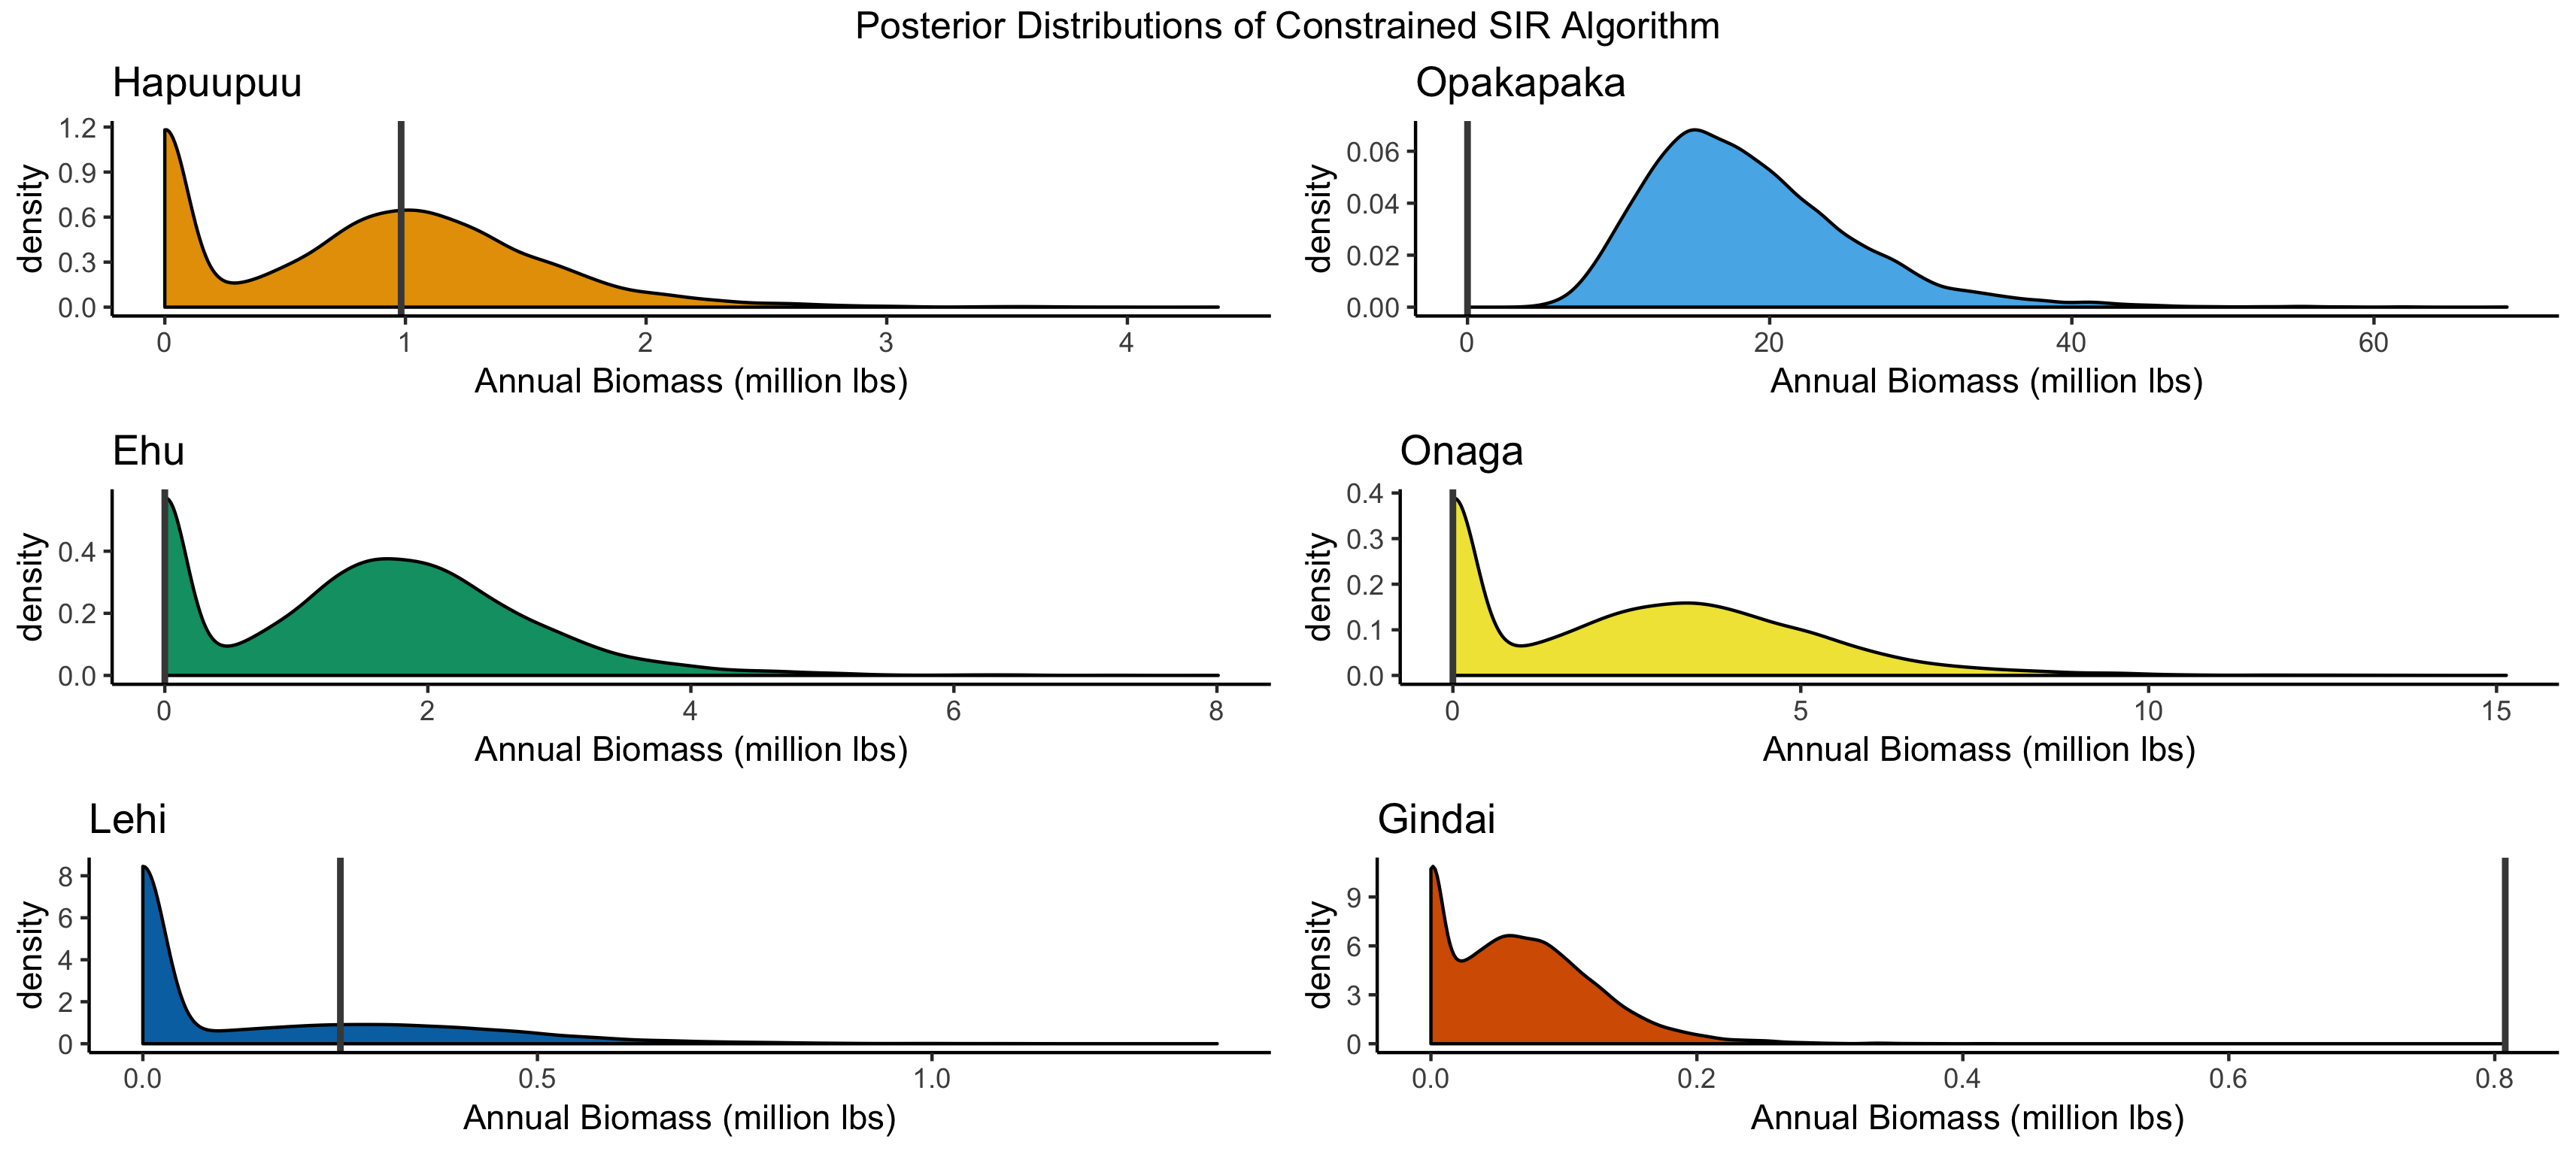
\includegraphics[width=\textwidth]{fig/post_constrained_sir}
    \caption{Histogram of the predicted biomass values from the posterior distribution for the six species at trophic level 4. These values were calculated from the Bayesian model that utilized the ecological constraint within the SIR algorithm. Plot created using R v.3.4.3 \cite{Rcite} ggplot2 package v.2.2.1 \cite{ggplot}.}
    \label{postconstsir}
\end{figure}

\begin{figure}[H]
     \centering
       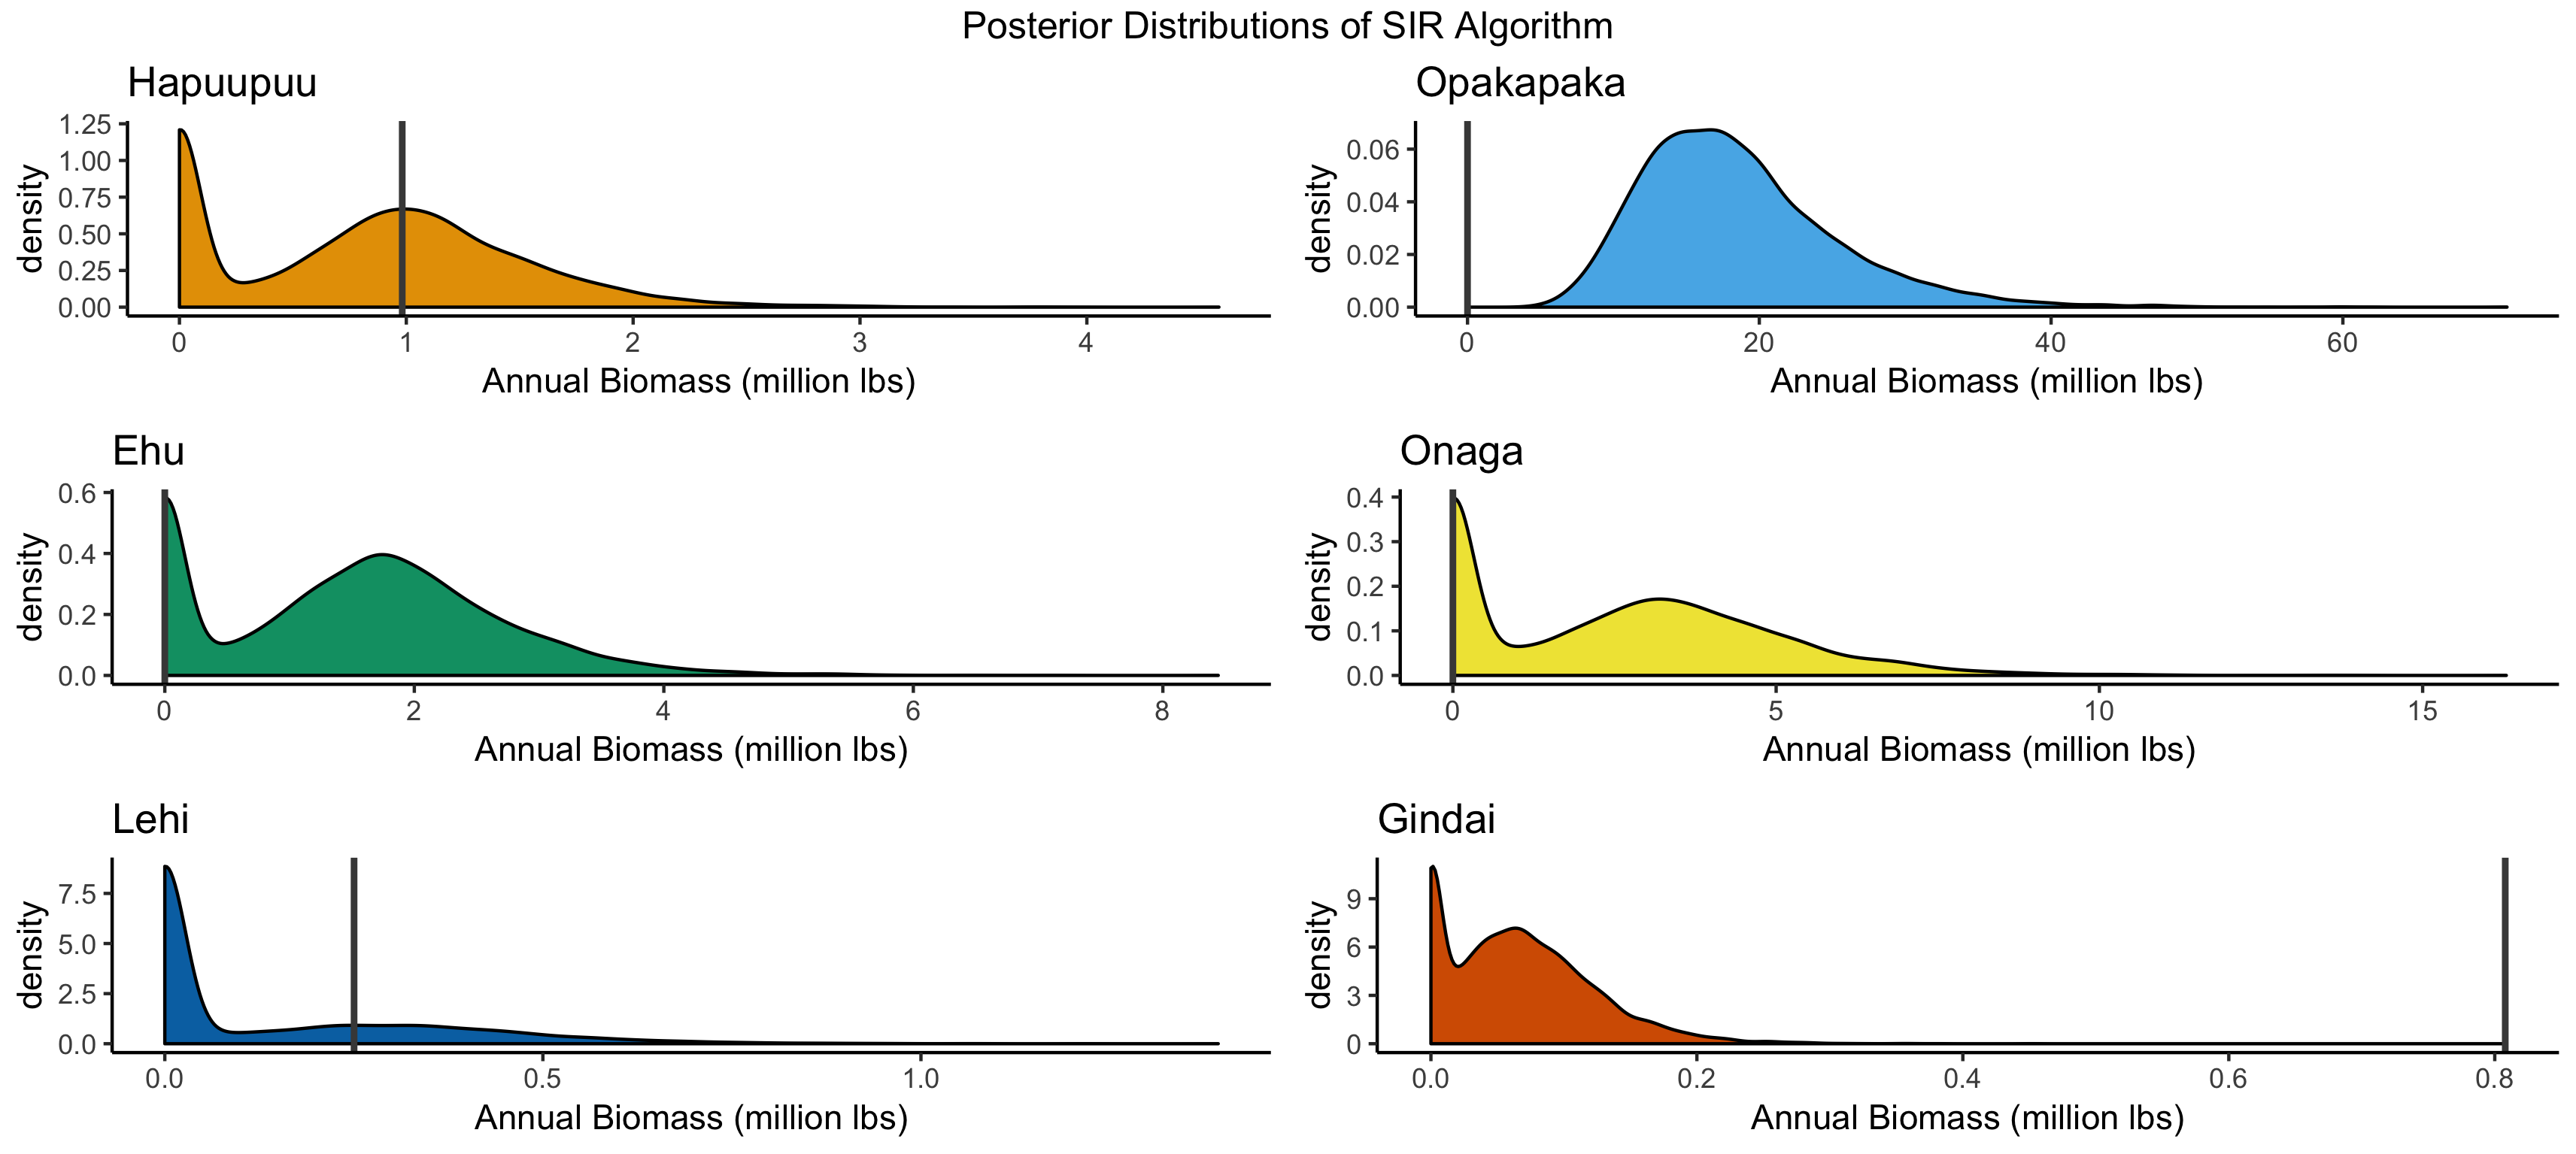
\includegraphics[width=\textwidth]{fig/post_sir}
    \caption{Histogram of the predicted biomass values from the posterior distribution for the six species at trophic level 4. These values were calculated from the Bayesian model using just the SIR algorithm. Plot created using R v.3.4.3 \cite{Rcite} ggplot2 package v.2.2.1 \cite{ggplot}.}
    \label{postsir}
\end{figure}

\begin{figure}[H]
     \centering
       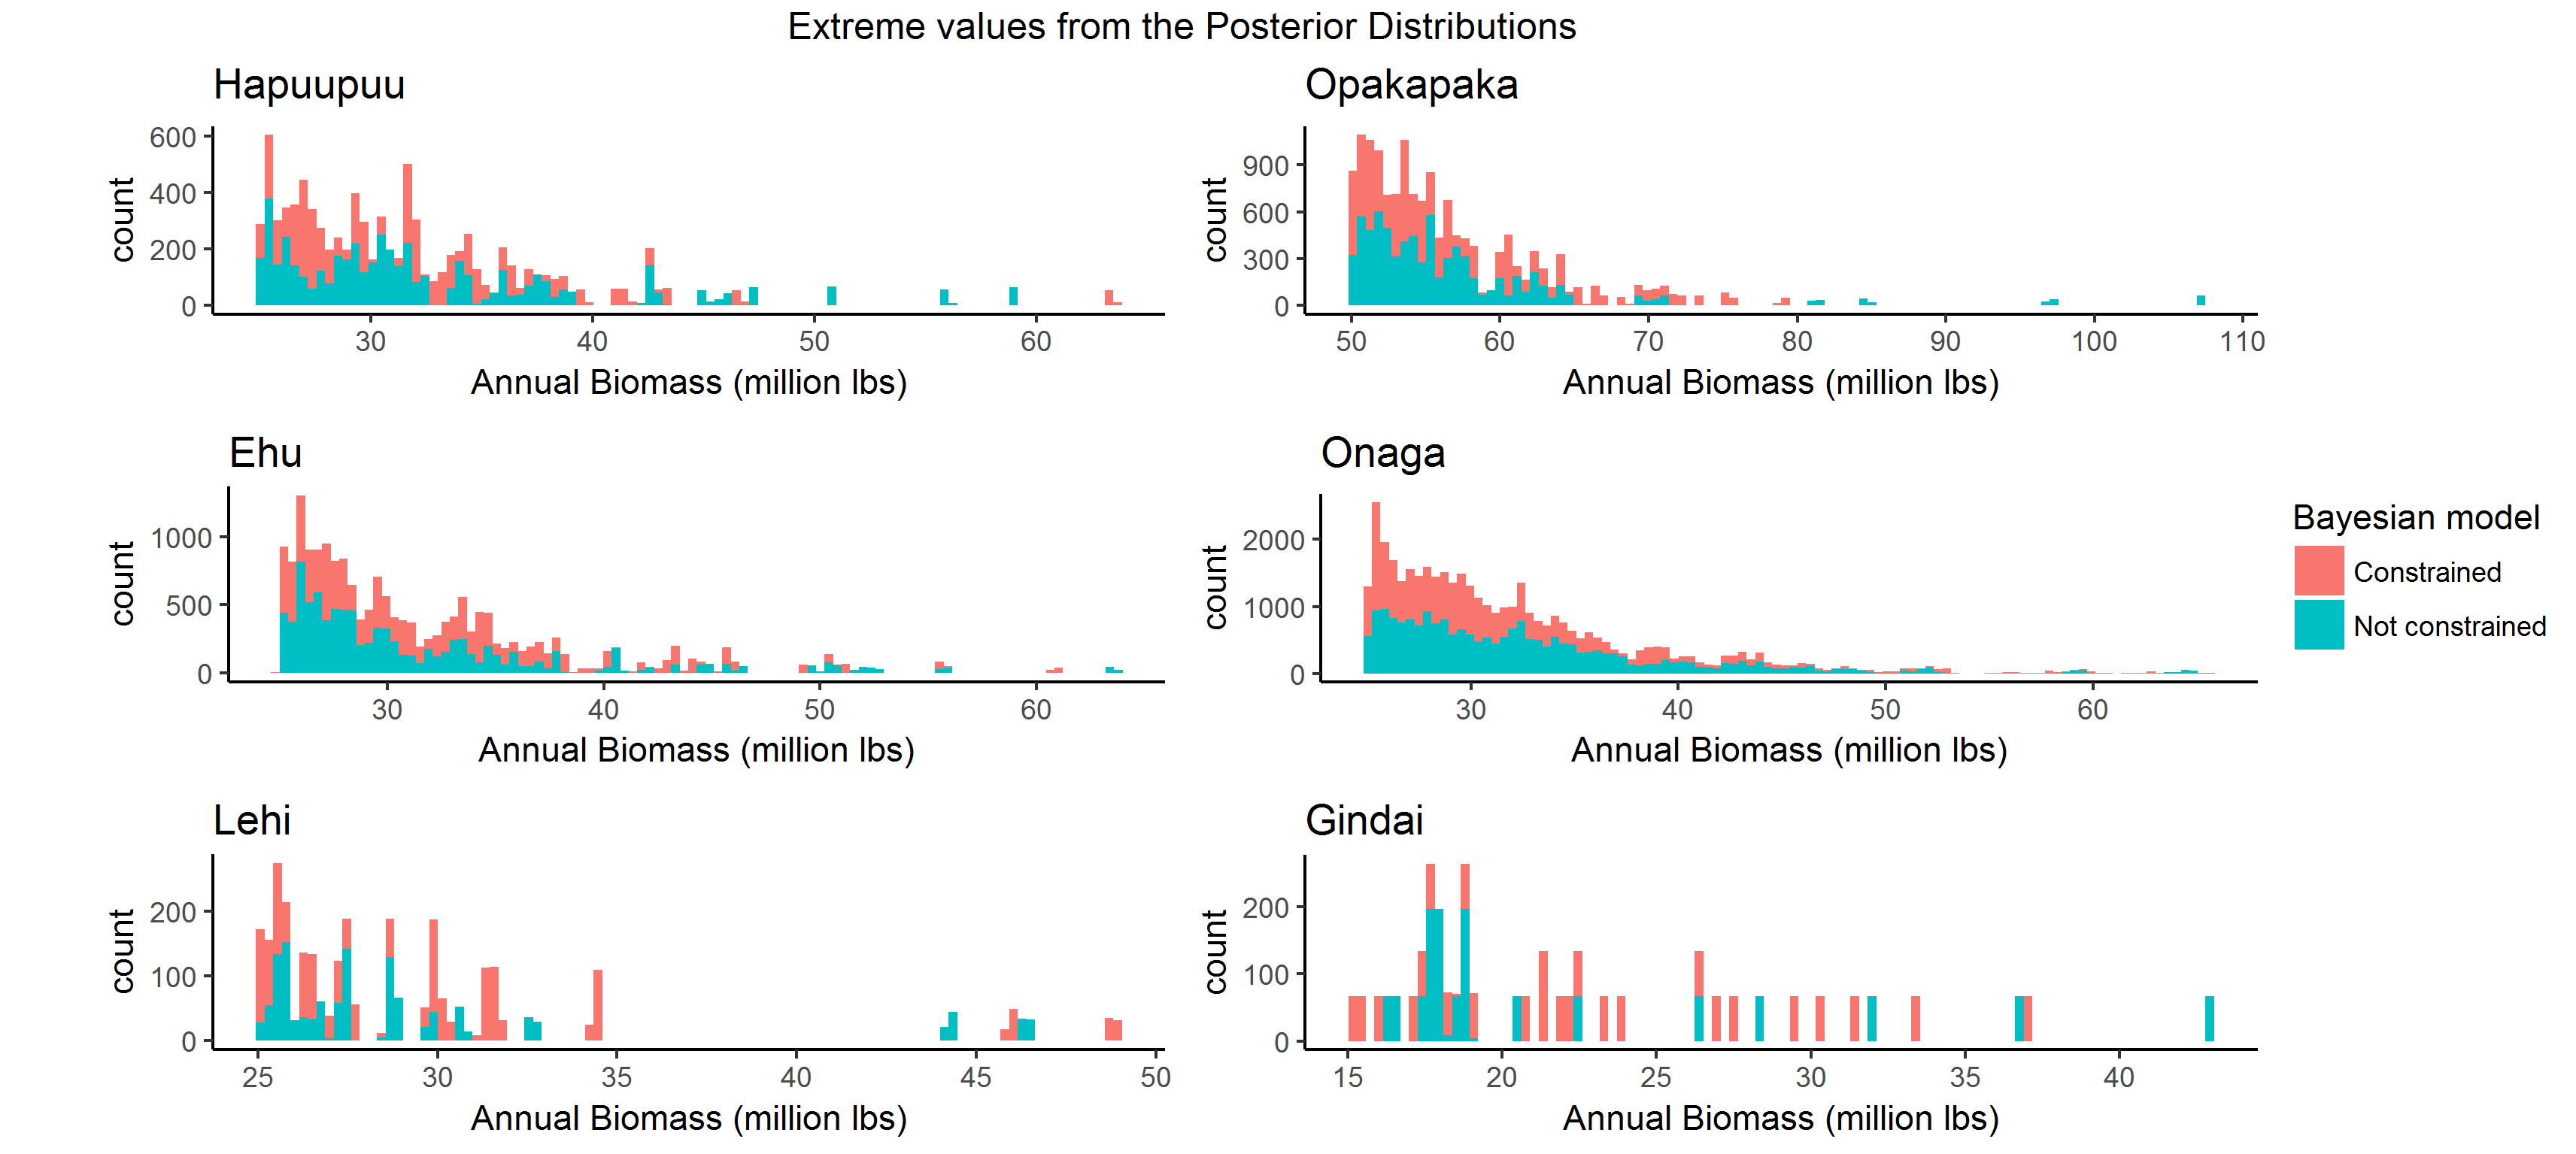
\includegraphics[width=\textwidth]{fig/post_ext}
    \caption{Histogram of the extreme predicted biomass values from the posterior distribution for the six species at trophic level 4. We adjusted the x-axis to visualize only the rare events. The original range extends out further. Plot created using R v.3.4.3 \cite{Rcite} ggplot2 package v.2.2.1 \cite{ggplot}.}
    \label{postext}
\end{figure}


\section*{Discussion}
As discussed above, modeling species as a complex assumes they share life history traits. When this assumption is invalid, we risk the chance of overestimating the abundance for some or all of the species in the complex. One of the Deep7 Bottomfish species, Opakapaka, makes up the majority of the catch composition (Fig. \ref{catchandcpue}). Based upon the assumptions in our model, our results suggests that Opakapaka has a drastically different distribution in relation to the other five species found at trophic level four. While the catch rates may be set at a level that is sustainable for Opakapaka, there is a chance that the ``weaker” stocks (e.g., Hapuupuu, Ehu, Onaga, Lehi, and Gindai) in this complex could be overfished and driven to unsustainably low levels \cite{hastings2017marine}. As a result, we are concerned that the assumption that species in the Deep7 Bottomfish Complex have similar life history traits is potentially invalid, which compromises the results and management suggestions made by the stock assessment.

\vspace{5mm}

We found that the Bayesian models are extremely sensitive to initial starting conditions. We theorize this could be due to a few reasons. We hypothesize that we need to improve our understanding of ecological data. From Chapter 3: Untangling uncertainty in food web models, we obtained a relatively large distribution of trophic level biomass. Our results would be more definite, if we had a narrower range for the trophic level biomass. Another explanation is that this method would be better suited for data-rich fisheries. Even without the ecological knowledge, the posterior distribution for the six species at trophic level 4 gave large distributions of biomass. Future work will test this modeling approach on a data-rich fishery.

\vspace{5mm}

While the inclusion of ecological information gave inconclusive results, the way we split up the aggregated data has potential application in fisheries. We pulled apart and obtained species-level information when the data was originally clustered. We were able to calculate species-specific estimates of carrying capacity in contrast with the aggregated estimate currently available for the fishery through the use of hyperpriors and hyperparameters. We argue the use of hyperpriors and hyperparameters for breaking apart the aggregate carrying capacity into its individual components can help data-limited fisheries move away from assessing the fishery as a complex to instead assessing the individual species. 

\vspace{5mm}
 
The inclusion of ecological information in the Bayesian production models did not always constrain the single-species model selection process. The presence of ecological information truncated off some of the largest estimated carrying capacity and biomass values, but not for every species (Fig. \ref{postext}). This finding is counter intuitive to what many ecologists and fisheries scientists believe. In theory, ecological knowledge would inform fisheries models and help ground truth the recommended sustainable removals by removing the unrealistic estimates. Our results found that single-species models are performing just fine. Thus in contrast to what some believe, perhaps incorporating ecosystem knowledge into fisheries management is not that necessary.
 
\subsection*{Limitations of Model}
We also placed an assumption about the starting biomass in the production model. Even though the locals have fished the Hawaiian bottomfish for hundreds of years, we assume unfished/virgin biomass in the start of the commercial fishery in year 1949. We are assuming that before modern technology, the effect of small-scale and artisanal fishing did not impact the populations enough to move it away from its natural unfished state. 

\vspace{5mm}

In general, our current carrying capacity estimates are conservative since we include only a subset of species. In the constrained Bayesian framework, we argued that the carrying capacity for the six bottomfish species could not exceed the trophic level four biomass. However, we acknowledge that more than just six species exist at trophic level four. If more species found in trophic level four were included, we would have even more information on what are reasonable carrying capacity estimates. 





%=== Appendix ============================================
\appendix

\dsp

\chapter{Appendix for Chapter 2: Tangled is the web we weave}{\label{appendix:a}}

\section{Decision trees}
We used regression trees with pruning, bagging, and random forests on the marine data set and trained the classifiers on 75\% of the marine transfer data. We tried different tree-based methods which involve stratifying or segmenting the predictor space (i.e., transfer efficiency) into a number of simple regions. Though the simple tree-building process may produce good predictions on our training data, it is likely to over fit the data, leading to poor test set performance. Thus, a better strategy is to grow a very large tree, and then prune it in order to obtain a subtree. We also tried other tree methods, such as bagging and random forests. These methods grow multiple trees which are then combined to yield a single consensus prediction. Combining a large number of trees can often result in dramatic improvements in prediction accuracy and reduce variance, at the expense of some loss in interpretation. For bagging, we construct regression trees using 1,000 bootstrapped training datasets. Random forest builds on the idea of bagging, but de-correlates the trees, thus leading to more reduction in variance. We build a 1,000 decision trees on bootstrapped training sample, but in the tree building process, each time a split in a tree is considered, a random sample of 2 predictors is chosen as split candidates from the full set of 3 predictors.

\vspace{5mm}

We selected the optimal number of number of nodes using cross validation. The best subtree with the minimized error had three nodes. The final subtree is visualized in Figure \ref{tree} and illustrates that combinations of specific factors can lead to distinct transfer efficiencies. It shows that trophic level is the most important factor in predicting transfer efficiency and that certain trophic levels have higher and lower transfer efficiencies. It also indicates that different regions in the ocean impact transfer efficiency at the primary consumer level. 

\begin{figure}[H]
     \centering
       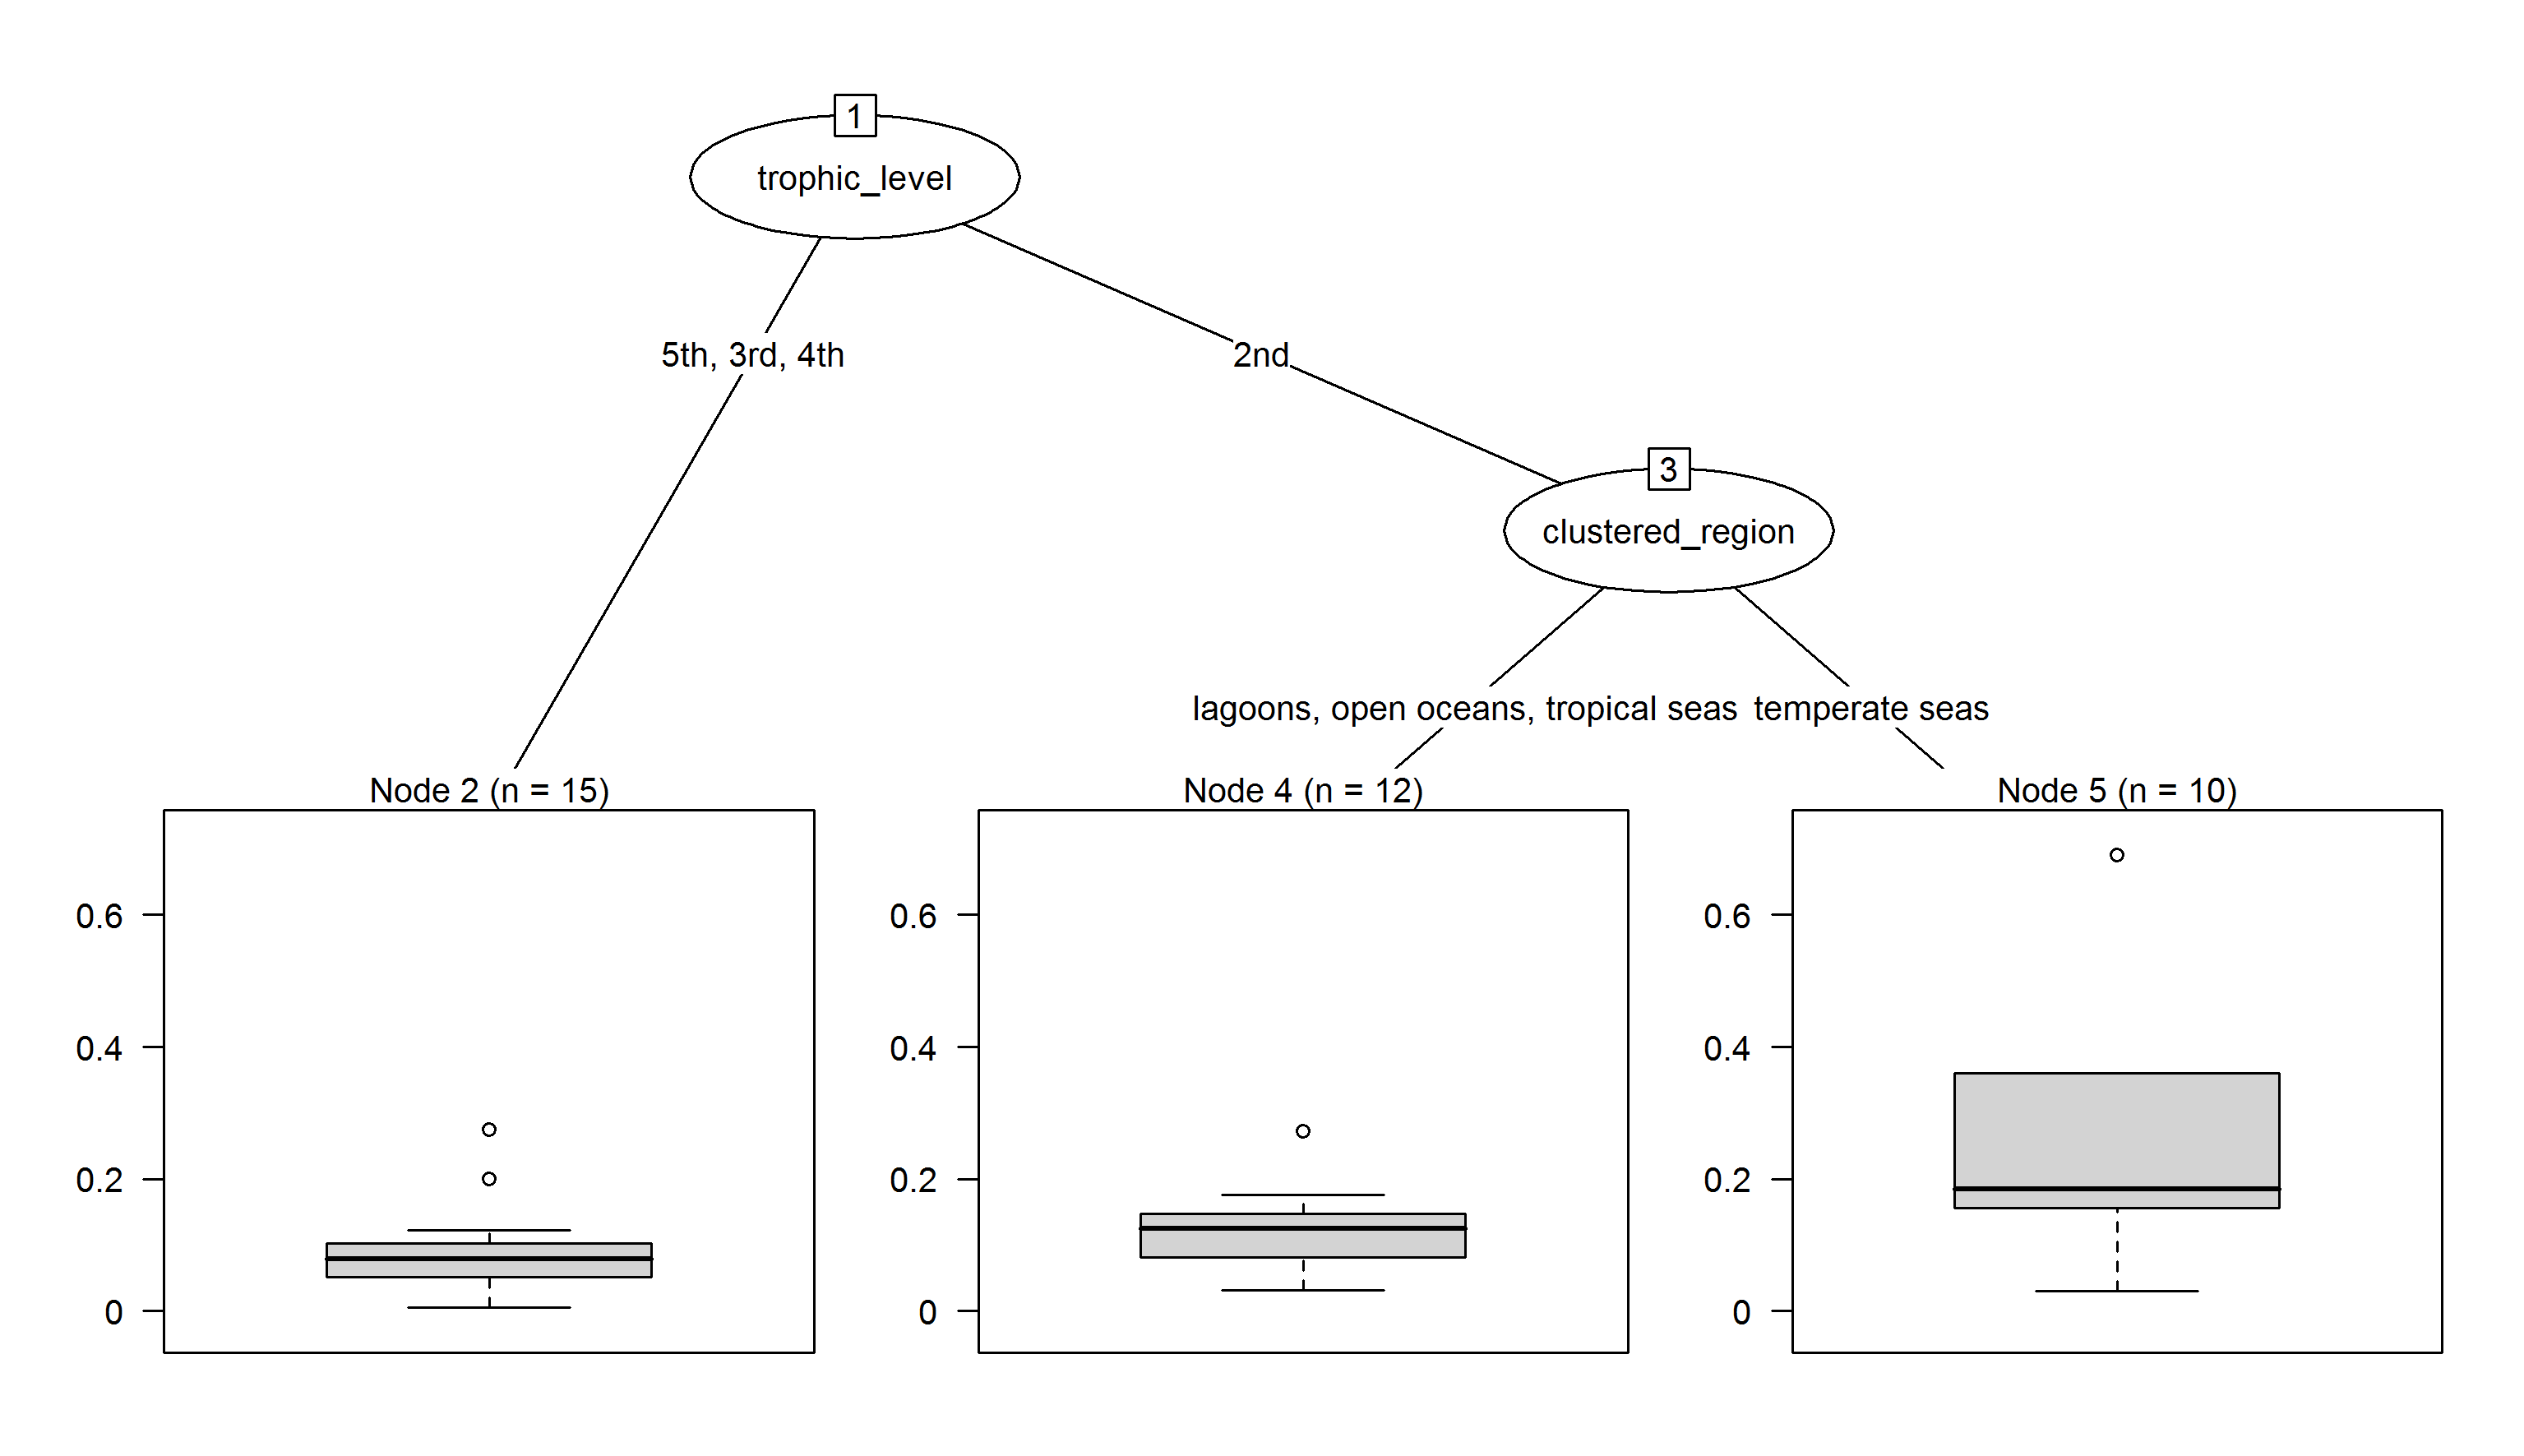
\includegraphics[width=\textwidth]{fig/tree}
    \caption{Visualization of regression tree with pruning ending in three terminal nodes. The tree stratifies transfer efficiency into three segments: when the transfer efficiency applies to either secondary, tertiary, and quaternary consumers, when the transfer applies to primary consumers and the region is either a lagoon, open ocean, or tropical shelves and seas, and when the transfer efficiency applies to primary consumers and the region is temperate shelves and seas. Plot created using R v.3.4.3 \cite{Rcite} partykit package v.1.2-2 \cite{hothorn2015partykit}.}
    \label{tree}
\end{figure}

\section{Fitting approximate distributions}
In the Monte Carlo simulations, we randomly drew from an approximate distribution that was fitted to the marine transfer efficiency data. In order to determine an approximate distribution for the marine transfer efficiency data, we ran goodness-of-fit tests. We started off with a skewness-kurtosis plot (Figure \ref{cf_te_a1}) to initially decide which distributions to consider (i.e., Beta and Gamma) \cite{fitdistrplus}. Then we fitted individual distributions to the data using maximum likelihood estimation and compared density plots of the fitted distributions to the histogram of the empirical distribution, a cumulative distribution (CDF) plot of both the empirical distribution and the fitted distributions, Q-Q plots, and P-P plots (Figure \ref{gof_te_a1}). Lastly, we used both AIC and BIC criterion to choose the most approximate distribution (Table \ref{te_aic_a1}). While the Gamma distribution was a reasonable choice. We preferred the Beta distribution because, like percentages, it is defined within the range [0, 1]. Therefore, we concluded that a $Beta(\alpha = 1.90, \beta = 13.36$) distribution was the most appropriate approximate distribution. 

\begin{table}[H]
\centering
\caption{Goodness-of-fit criteria for transfer efficiency data}
\begin{tabular}{r|c|c}
  \hline \small
 Goodness-of-fit criteria & Beta  & Gamma \\ 
   \hline
   Akaike's Information Criterion (AIC) & -354.94 & -369.97 \\   
   Bayesian Information Criterion (BIC) & -348.96 &  -363.99  \\
   \hline
\end{tabular} 
\label{te_aic_a1}
\end{table}

\begin{figure}[H]
     \centering
       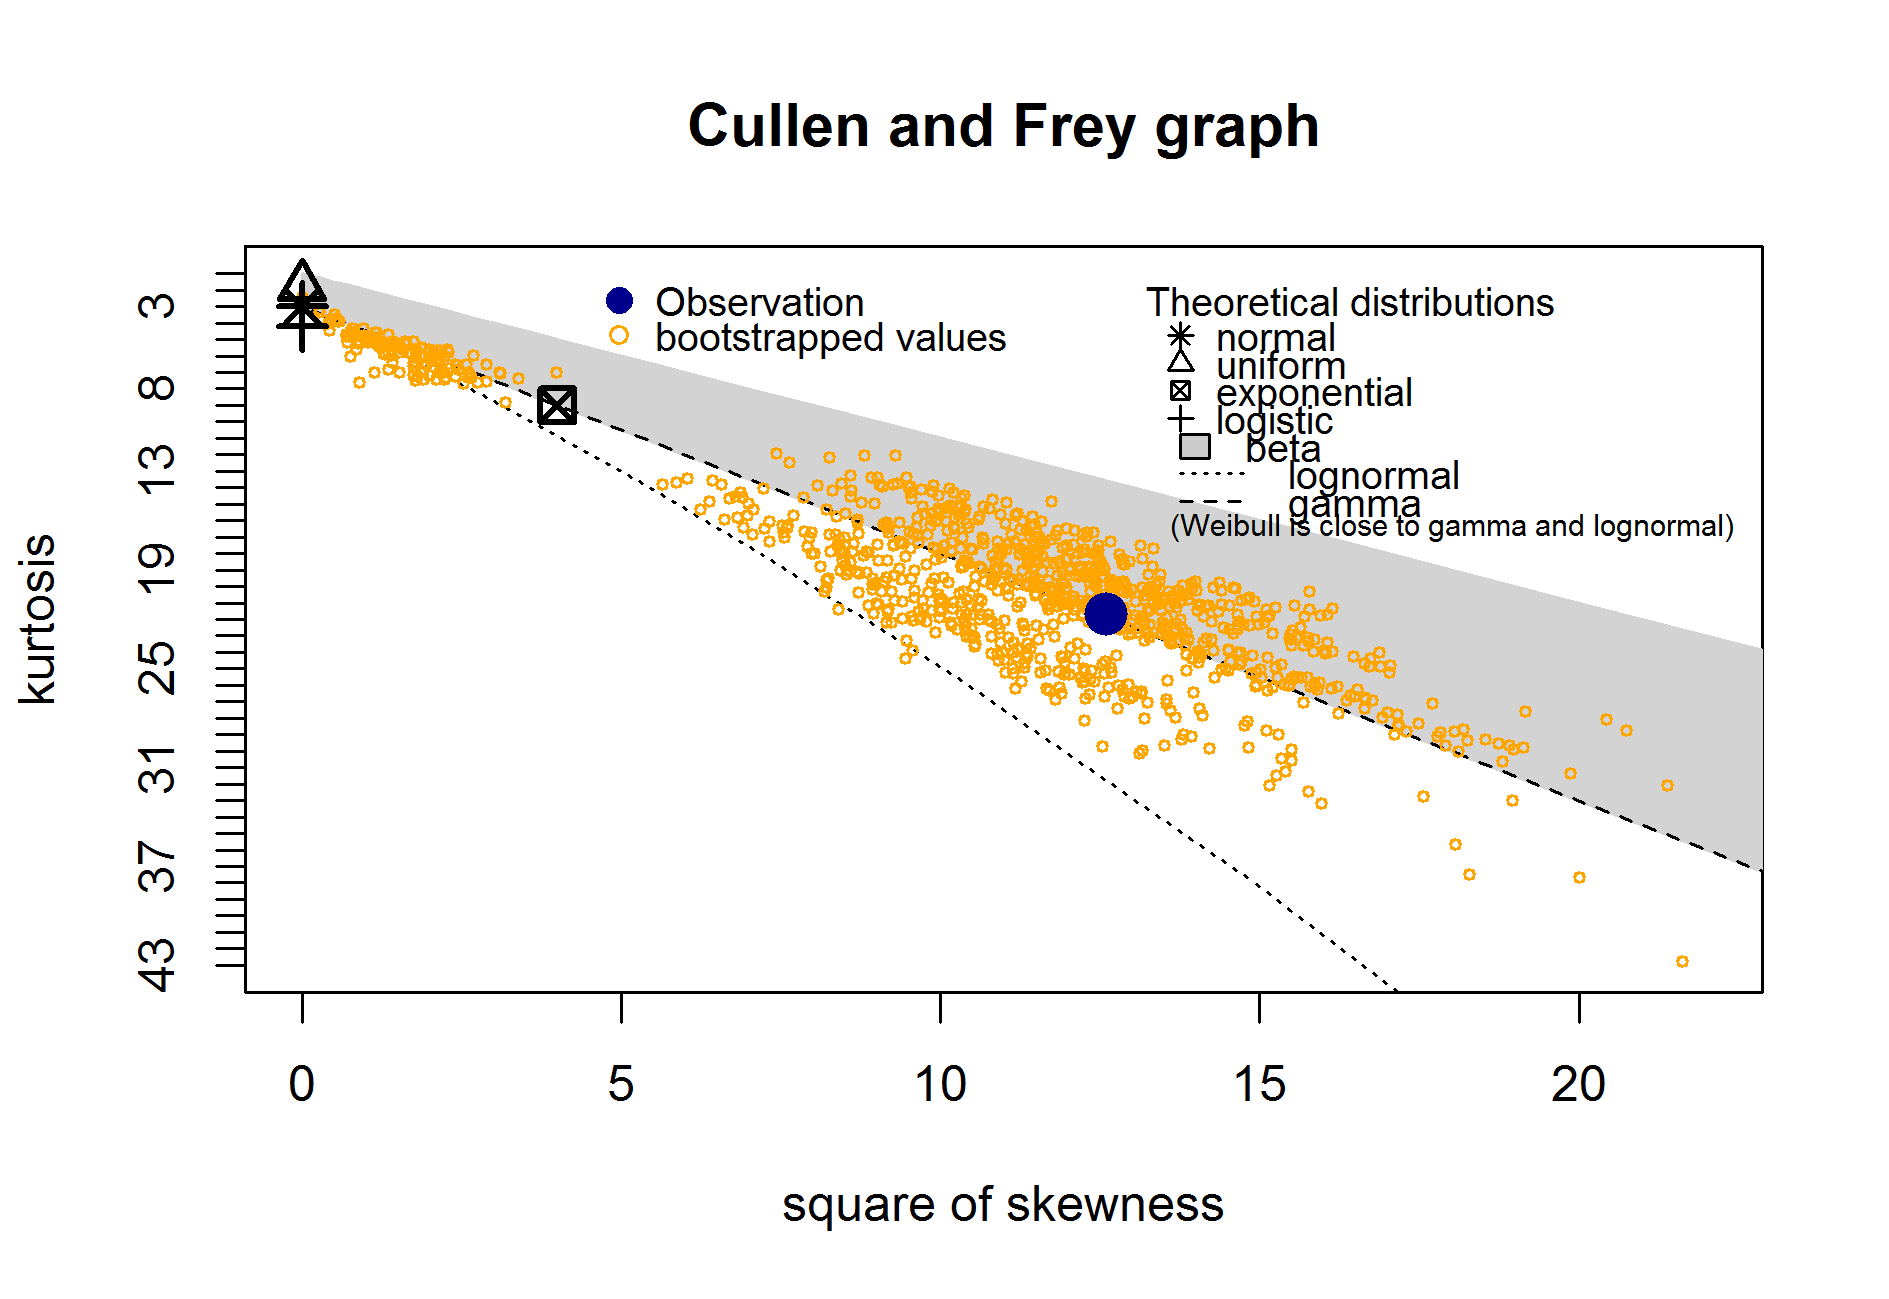
\includegraphics[width=.8\textwidth]{fig/cullen_frey_te}
    \caption{Visualizes all potential continuous distributions against the marine transfer data and bootstrapped data. The figure shows it potentially follows a Beta and Gamma distribution. Plot created using R v.3.4.3 \cite{Rcite} fitdistrplus package v.$1.0-9$ \cite{fitdistrplus}. }
    \label{cf_te_a1}
\end{figure}

\begin{figure}[H]
     \centering
       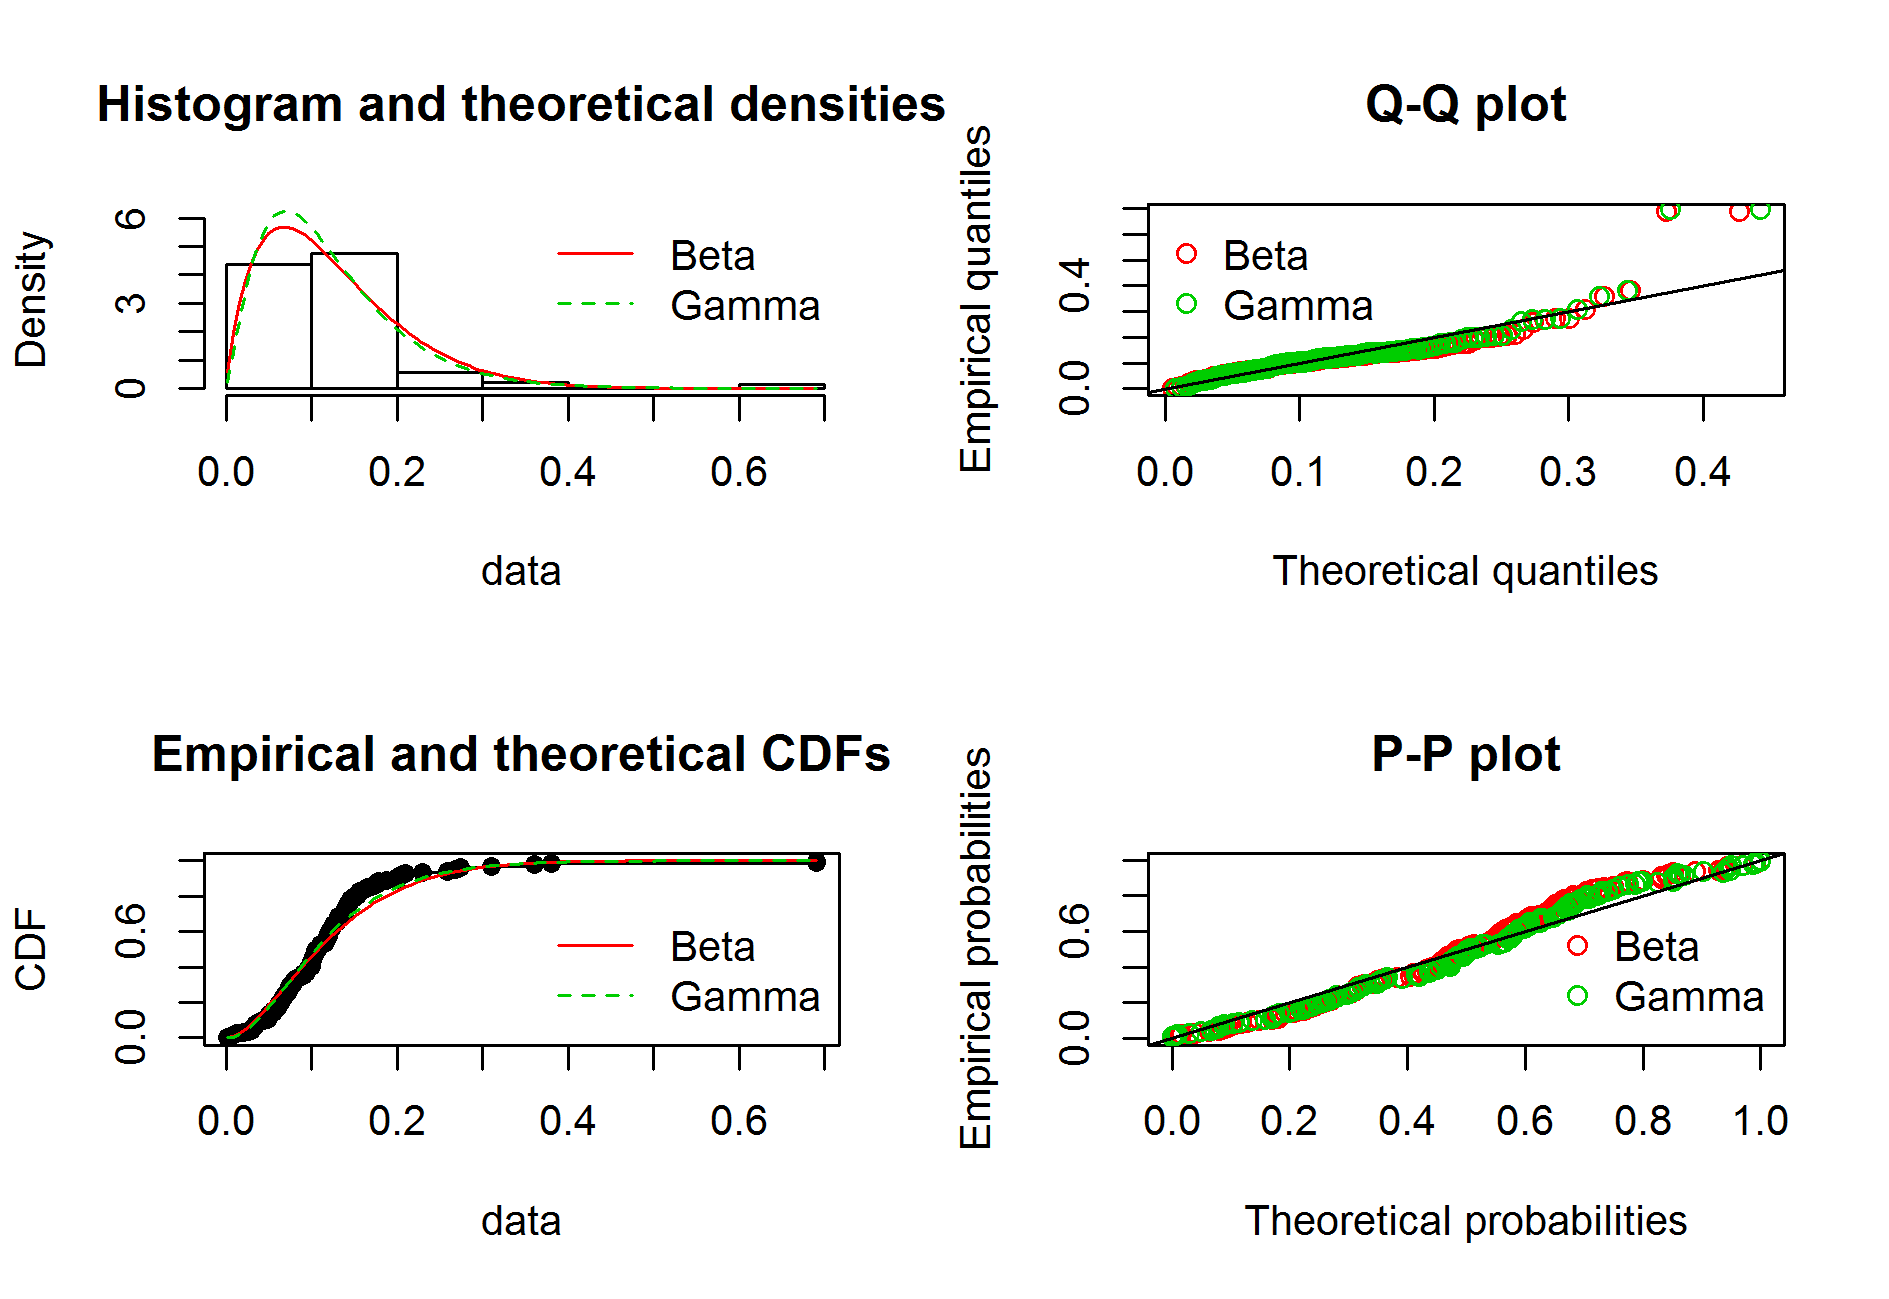
\includegraphics[width=.8\textwidth]{fig/gof_te}
    \caption{Density plots of the fitted distributions to the histogram of the empirical distribution using the marine transfer efficiency data, a CDF plot of both the empirical distribution and the fitted distributions (for the Beta and Gamma choices), Q-Q plots, and P-P plots. Plot created using R v.3.4.3 \cite{Rcite} fitdistrplus package v.$1.0-9$ \cite{fitdistrplus}. }
    \label{gof_te_a1}
\end{figure}

\section{SeaWiFS}
We used 8-day time series Sea-viewing Wide Field-of-view Sensor (SeaWiFS) chlorophyll \textit{a} data from 1997 to 2010 that was transformed using the Vertically Generalized Production Model (VGPM) to estimate net primary production (NPP) from chlorophyll \textit{a} \cite{behrenfeld1997photosynthetic}. The SeaWiFS data were originally obtained from the Oregon State Ocean Productivity website (\url{http://www.science.oregonstate.edu/ocean.productivity}). They use a gap filling algorithm to populate missing pixels due to cloud coverage; however if no good data is available, pixels remain empty. We segmented the SeaWiFS data using the boundaries of the California Current and assumed a closed system at equilibrium. The data then were converted from 8 day averages in mg C / $m^2 $/ day per 9 km x 9 km pixel into total metric tons of Carbon per year total across the entire region. Although from 1997 to 2010 SeaWiFS collected data every 8 days per 9 km x 9 km pixel, the time series had gaps due to machine parts malfunctioning. Therefore, the updated data set used for our analysis contained observations only from 1998-2007. From there we fit an ARIMA model to calculate the mean (505210291 tons of C/year) of the time series. 

\section{R packages and versions}
To promote reproducibility, we include a list of all R packages and versions used in this analysis.

\begin{itemize}
\item astsa package v.1.8 \cite{astsa}
\item dplyr package v.0.7.5 \cite{wickham2015dplyr}
\item fitdistrplus package v.$1.0-9$ \cite{fitdistrplus}
\item forecast package v8.2 \cite{forecast1, forecast2} 
\item ggplot2 package v.2.2.1 \cite{ggplot}
\item gridExtra package v.2.3 \cite{gridextra}
\item partykit package v.1.2-2 \cite{hothorn2015partykit}
\item R v.3.4.3 \cite{Rcite} 
\item randomForest v.4.6-12 \cite{liaw2016classification}
\item rpart package v.4.1-11 \cite{therneau2015rpart}
\item tree package v.1.0-37 \cite{ripley2016tree}
\end{itemize}


\chapter{Appendix for Chapter 3: Untangling uncertainty in food web models}{\label{appendix:b}}

\subsection{SeaWiFS}
\subsubsection{Time Series Analysis}
To create Case 1 ($f^1(\nu)$) in the trophic pyramid food web model where $\nu$ is a fixed constant, we used 8-day time series Sea-viewing Wide Field-of-view Sensor (SeaWiFS) chlorophyll \textit{a} data from 1997 to 2010 that was transformed using the \textit{Eppley-}Vertically Generalized Production Model (VGPM) to estimate net primary production (NPP) from chlorophyll \textit{a}. The \textit{Eppley-}VGPM estimates were used rather than the VGPM data since temperatures surrounding the main Hawaiian Islands (MHI) are above $20^{\circ}$C \cite{morel1991pigment, antoine1996oceanic, stock2017reconciling}. The SeaWiFS data were originally obtained from the Oregon State Ocean Productivity website (\url{http://www.science.oregonstate.edu/ocean.productivity/}). They use a gap filling algorithm to populate missing pixels due to cloud coverage; however if no good data is available, pixels remain empty. We segmented the SeaWiFS data using the exclusive economic zone (EEZ) boundaries of the MHI and assumed a closed system at equilibrium (Fig. \ref{A2:SeaWiFSmhi}). The data then were converted from 8 day averages in mg C / $m^2$ / day per 9 km x 9 km pixel into total metric tons of Carbon per year total across the entire MHI. Although from 1997 to 2010 SeaWiFS collected data every 8 days  per 9 km x 9 km pixel, the time series had gaps due to machine parts malfunctioning. Therefore, the updated data set used for our analysis contained observations only from 1998-2007. 

\begin{figure}[H]
     \centering
       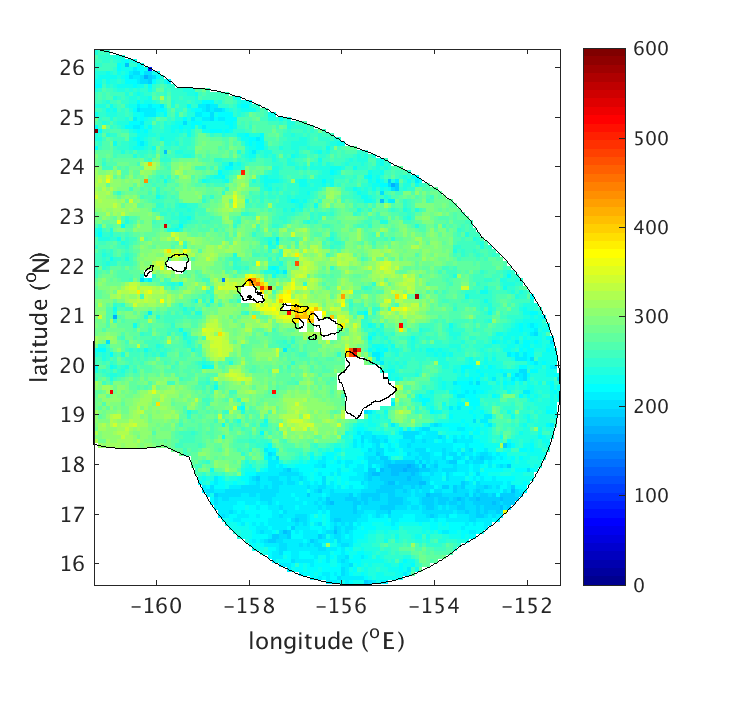
\includegraphics[width=.7\textwidth]{fig/SeaWiFSmhi}
    \caption{A single 8-day time frame of the SeaWiFS \textit{Eppley-}VGPM NPP data in January 1998 for the main Hawaiian Islands EEZ. The color scale shows the amount of estimated NPP in total gigatons of Carbon per year per pixel. The pixel size of the SeaWiFS data set is 9 by 9 km.}
    \label{A2:SeaWiFSmhi}
\end{figure}

Since the SeaWiFS data were collected over time, we started off by verifying that there was a violation of independence and then chose a usable time series model. The NPP data demonstrated a strong annual frequency, a smaller six month frequency, and were non-stationary in the trend and seasonality (See Fig. \ref{A2:SeaWiFSmhi_eda1}  and \ref{A2:SeaWiFSeda3}). This was not surprising since most biological data sets are seasonal and are influenced by the time of year. 

\begin{figure}[H]
     \centering
       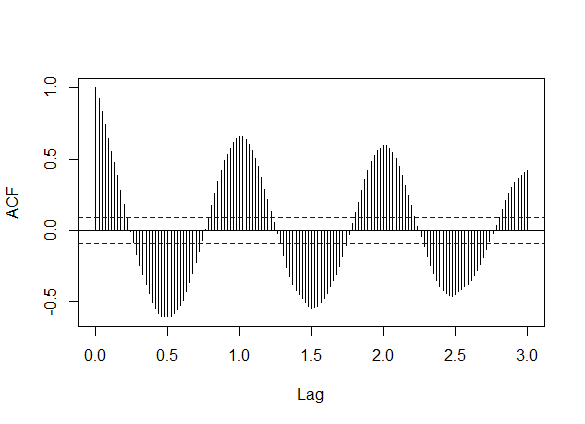
\includegraphics[width=.7\textwidth]{fig/seawifs_acf}
    \caption{ACF plot of SeaWiFS data. Plots created using R v.3.4.3 \cite{Rcite} forecast package v8.2 \cite{forecast1, forecast2}.}
    \label{A2:SeaWiFSeda1}
\end{figure}

\begin{figure}[H]
     \centering
       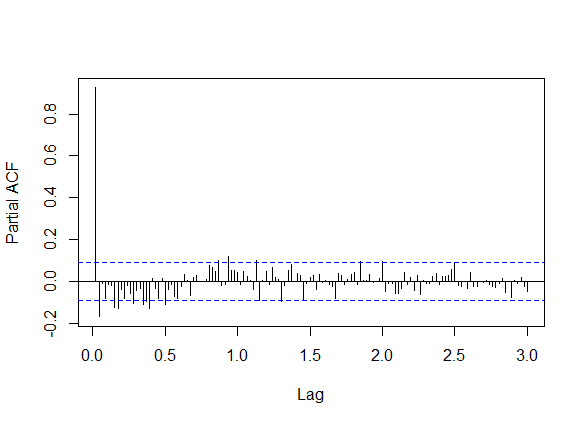
\includegraphics[width=.7\textwidth]{fig/seawifs_pacf}
    \caption{PACF plots of SeaWiFS data. Plots created using R v.3.4.3 \cite{Rcite} forecast package v8.2 \cite{forecast1, forecast2}.}
    \label{A2:SeaWiFSeda2}
\end{figure}

\begin{figure}[H]
     \centering
       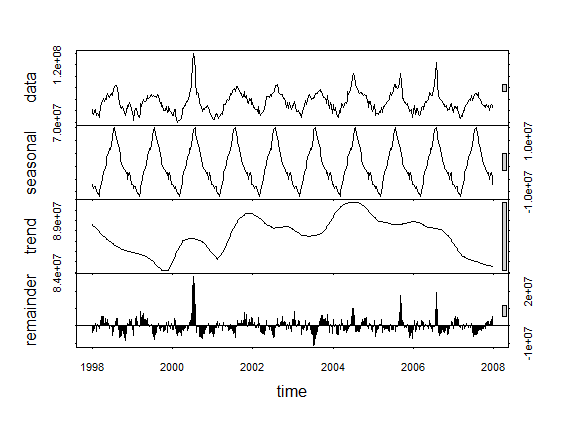
\includegraphics[width=.7\textwidth]{fig/seawifs_periodic}
    \caption{Exploratory time series plots of SeaWiFS data--seasonal and trend components. Plots created using R v.3.4.3 \cite{Rcite} forecast package v8.2 \cite{forecast1, forecast2}.}
    \label{A2:SeaWiFSeda3}
\end{figure}

We fitted a seasonal autoregressive integrated moving average model, or \\ SARIMA$(0,0,2)(0,0,2)_{46}$ to the pre-processed SeaWiFS NPP data (i.e., moving average order $q = 2$, seasonal moving average $Q = 2$, and seasonal component $s = 46$ (365 days/8-day time series = 46)).

\begin{equation} \label{sarima}
X_t = \delta + (1 + \theta_1B + \theta_2B^2)(1 + \Theta_1B^{46} + \Theta_2B^{92})W_t
\end{equation}

In Eq. \ref{sarima}, $X_t$ is the total NPP estimated across the MHI in 8-day time periods from 1998-2007 where $t \in$ \{1, 460\}, $\delta$ represents the mean of the time series, $\theta_1$ and $\theta_2$ are the moving average parameters, $\Theta_2$ and $\Theta_2$ are the seasonal moving average parameters, and $W_t \stackrel{iid}{\sim} N(0,\sigma_w^2)$. The backshift operator, B, is defined as $ BW_t  = W_{t-1}$, $B^2W_t  = W_{t-2}$, $B^{46}W_t  = W_{t-46}$, and $B^{92}W_t  = W_{t-92}$.  Our model, Eq. \ref{sarima}, was chosen based on information criteria. Parameters were estimated using maximum likelihood estimation \cite{forecast1, forecast2}. The parameter estimates can be found in Table \ref{sarima_parameters}. The estimate of parameter $\delta$ was used for the value of $\nu$ when it was treated as a fixed constant in the hierarchical food web model ($c_1$ in $f^1(\nu)$).

\begin{table}[H]
\centering
\caption{Seasonal ARIMA parameter estimates for Eq. \ref{sarima} and their respective standard error calculated using R v.3.4.3 \cite{Rcite} forecast package v8.2 and function auto.arima() \cite{forecast1, forecast2} }
\begin{tabular}{r|c|c}
  \hline \small
 Parameters & Estimates & Standard error \\ 
   \hline
   $\delta$ & 87339861.7 & 696375.7 \\   
   $\theta_1$ & 0.9806 & 0.0413 \\
   $\theta_2$ & 0.4817 & 0.0359 \\
   $\Theta_1$ & 0.3379 & 0.0470 \\
   $\Theta_2$ & 0.3392 & 0.0449 \\
   $\sigma_w^2$ & 1.494306e+13 & \\
   \hline
\end{tabular} 
\label{sarima_parameters}
\end{table}

\subsubsection{Simulation Setting}
While in Case 1 ($f^1(\nu)$) $\nu$ is treated as a fixed constant, in Case 2 ($f^2(\nu)$) $\nu$ is a random variable. In order to determine an approximate distribution for $\nu$, we ran goodness-of-fit tests on the SeaWiFS NPP data. We started off with a skewness-kurtosis plot (Fig. \ref{SeaWiFSgof}) to initially decide which distributions to consider (i.e., Lognormal, Weibull, and Gamma) \cite{fitdistrplus}. Then we fitted individual distributions to the data using maximum likelihood estimation and compared density plots of the fitted distributions to the histogram of the empirical distribution, a cumulative distribution (CDF) plot of both the empirical distribution and the fitted distributions, Q-Q plots, and P-P plots (Fig. \ref{SeaWiFSgof2}). Lastly, we used both AIC and BIC criterion to choose the most approximate distribution (Table \ref{seawifs_aic}). From there, we concluded that the Lognormal distribution was the most appropriate approximate distribution. The Lognormal distribution has two parameters $\mu$ and $\sigma^2$ and is defined within the range for $\nu > 0$. The probability distribution function (PDF) and equations for the mean and variance of a Lognormal distribution can be found in Table \ref{distributions}.

\begin{table}[H]
\centering
\caption{Goodness-of-fit criteria for SeaWiFS NPP data}
\begin{tabular}{r|c|c|c}
  \hline \small
 Goodness-of-fit criteria & Lognormal & Weibell & Gamma \\ 
   \hline
   Akaike's Information Criterion (AIC) & 15997.97 & 16192.32 & 16007.49 \\   
   Bayesian Information Criterion (BIC) & 16006.23 & 16200.58 & 16015.75 \\
   \hline
\end{tabular} 
\label{seawifs_aic}
\end{table}

\begin{figure}[H]
     \centering
       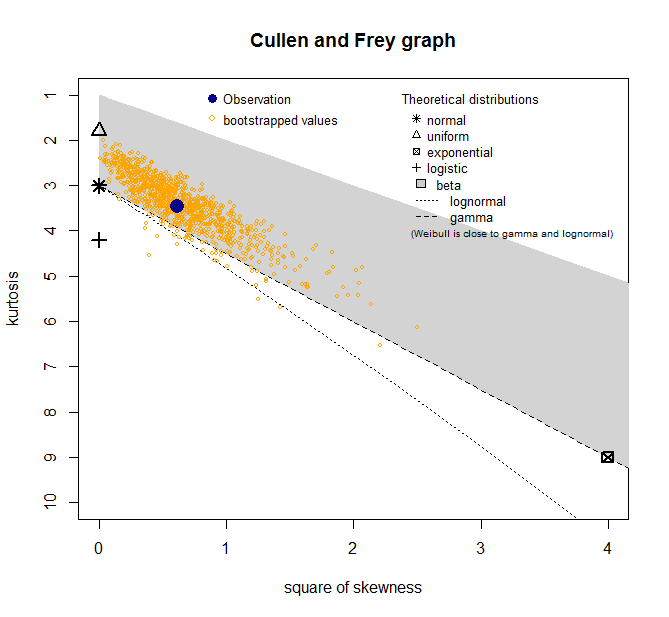
\includegraphics[width=.7\textwidth]{fig/Scen2gof}
    \caption{Visualizes all potential continuous distributions against the SeaWiFS data and bootstrapped data. The figure shows it potentially follows a Gamma, Weibull, and Lognormal distribution. It also appears Beta could be a reasonable choice, but the SeaWiFS data is not constricted between 0 and 1. Therefore Beta is ruled out as a potential distribution. Plot created using R v.3.4.3 \cite{Rcite} fitdistrplus package v.$1.0-9$ \cite{fitdistrplus}. }
    \label{SeaWiFSgof}
\end{figure}

\begin{figure}[H]
     \centering
       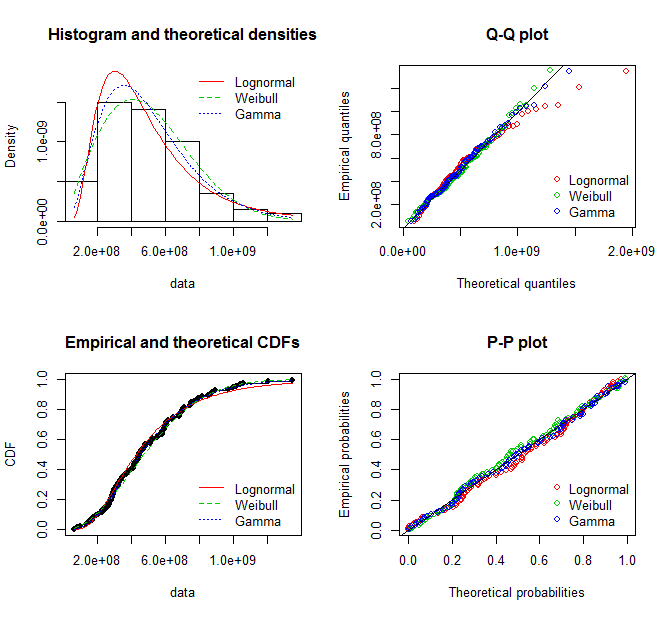
\includegraphics[width=.7\textwidth]{fig/Scen2gof2}
    \caption{Density plots of the fitted distributions to the histogram of the empirical distribution, a CDF plot of both the empirical distribution and the fitted distributions (Gamma, Weibull, and Lognormal), Q-Q plots, and P-P plots. Plot created using R v.3.4.3 \cite{Rcite} fitdistrplus package v.$1.0-9$ \cite{fitdistrplus}. }
    \label{SeaWiFSgof2}
\end{figure}

\subsection{Transfer Efficiency}
We utilized data gathered from a literature review on transfer efficiencies to fit approximate distributions for Case 2 and 3 of the transfer efficiencies ($\tau_h$). The data includes articles that mentioned both food web and transfer efficiency and then selected from these studies those that included data whether model-based or empirical. Case 2 used all of the marine data (i.e., both model-based and empirical) to fit a distribution. The resulting distributional assumption was placed on transfer efficiencies ($\tau_h$) for all trophic levels $h \in \{2, 3, 4\}$. Case 3 subsetted the marine transfer efficiency data by trophic level $h$ in order to place distinct distributional assumptions on transfer efficiencies at each trophic level. In order to determine approximate distributions for each of the cases, we ran goodness-of-fit tests. We started off with skewness-kurtosis plots (Fig. \ref{cf_te_a2}, \ref{cf_te2}, \ref{cf_te3}, and \ref{cf_te4}) to initially decide which distributions to consider (i.e., Beta and Gamma) \cite{fitdistrplus}. Then we fitted individual distributions to the data using maximum likelihood estimation and compared density plots of the fitted distributions to the histogram of the empirical distribution, a cumulative distribution (CDF) plot of both the empirical distribution and the fitted distributions, Q-Q plots, and P-P plots (Fig. \ref{gof_te_a2}, \ref{gof_te2}, \ref{gof_te3}, and \ref{gof_te4}). Lastly, we used both AIC and BIC criterion to choose the most approximate distribution (Table \ref{te_aic_a2}, \ref{te2_aic}, \ref{te3_aic}, and \ref{te4_aic}). While the Gamma distribution was a reasonable choice, we preferred the Beta distribution, because the transfer efficiency is a percentage and the Beta distribution is defined within the range [0, 1]. Therefore, we concluded that for both Case 2 and 3 the Beta distribution was the most appropriate approximate distribution. Each data set used in Case 2 and 3 have distinct values for the shape parameters $\alpha$ and $\beta$. The probability distribution function (PDF) and equations for the mean and variance of a Beta distribution can be found in Table \ref{distributions}.

\begin{table}[H]
\centering
\caption{Goodness-of-fit criteria for transfer efficiency data}
\begin{tabular}{r|c|c}
  \hline \small
 Goodness-of-fit criteria & Beta  & Gamma \\ 
   \hline
   Akaike's Information Criterion (AIC) & -354.94 & -369.97 \\   
   Bayesian Information Criterion (BIC) & -348.96 &  -363.99  \\
   \hline
\end{tabular} 
\label{te_aic_a2}
\end{table}

\begin{figure}[H]
     \centering
       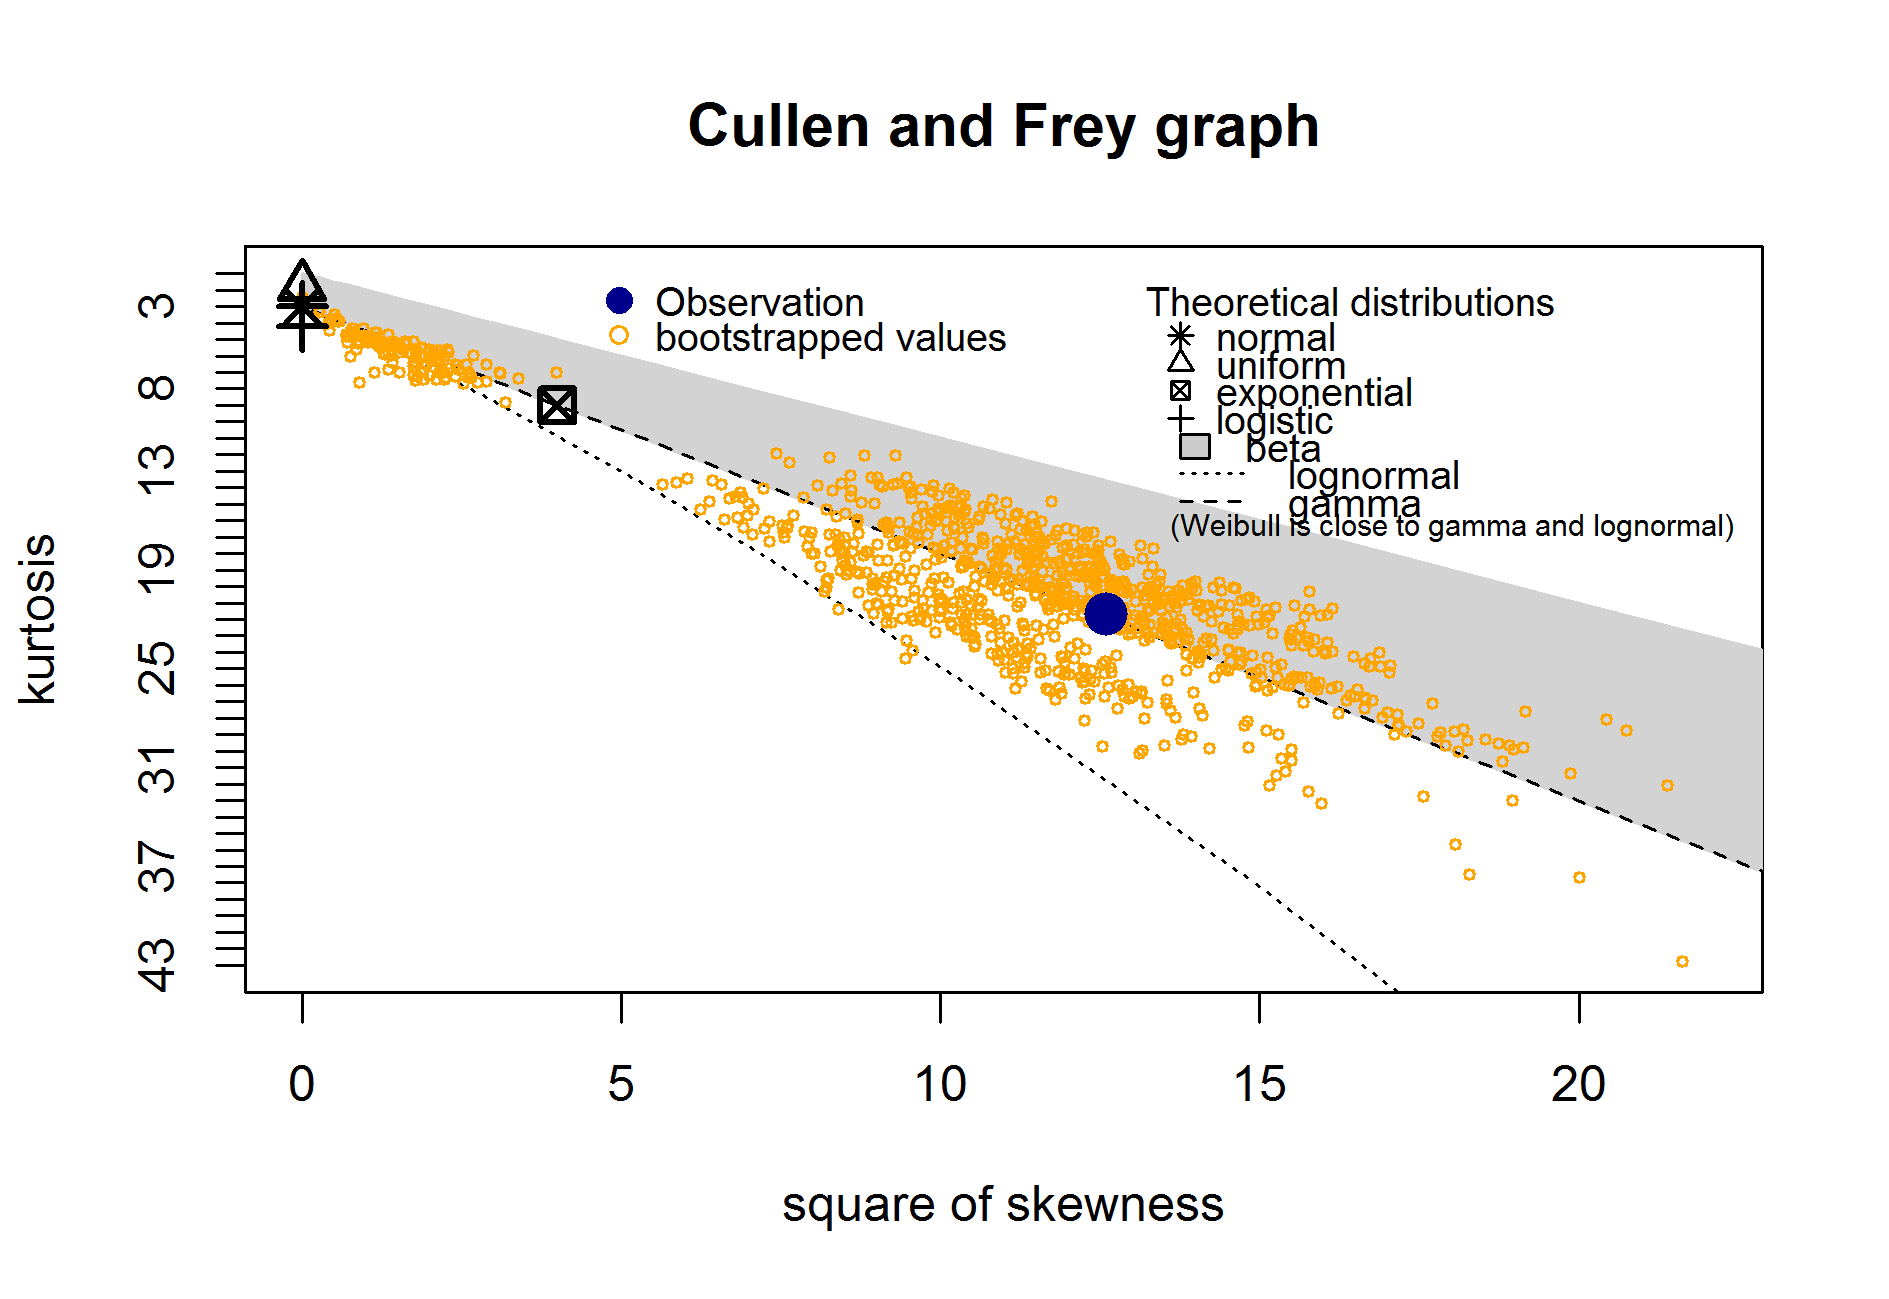
\includegraphics[width=.8\textwidth]{fig/cullen_frey_te}
    \caption{Visualizes all potential continuous distributions against the marine transfer data (Case 2) and bootstrapped data. The figure shows it potentially follows a Beta and Gamma distribution. Plot created using R v.3.4.3 \cite{Rcite} fitdistrplus package v.$1.0-9$ \cite{fitdistrplus}. }
    \label{cf_te_a2}
\end{figure}

\begin{figure}[H]
     \centering
       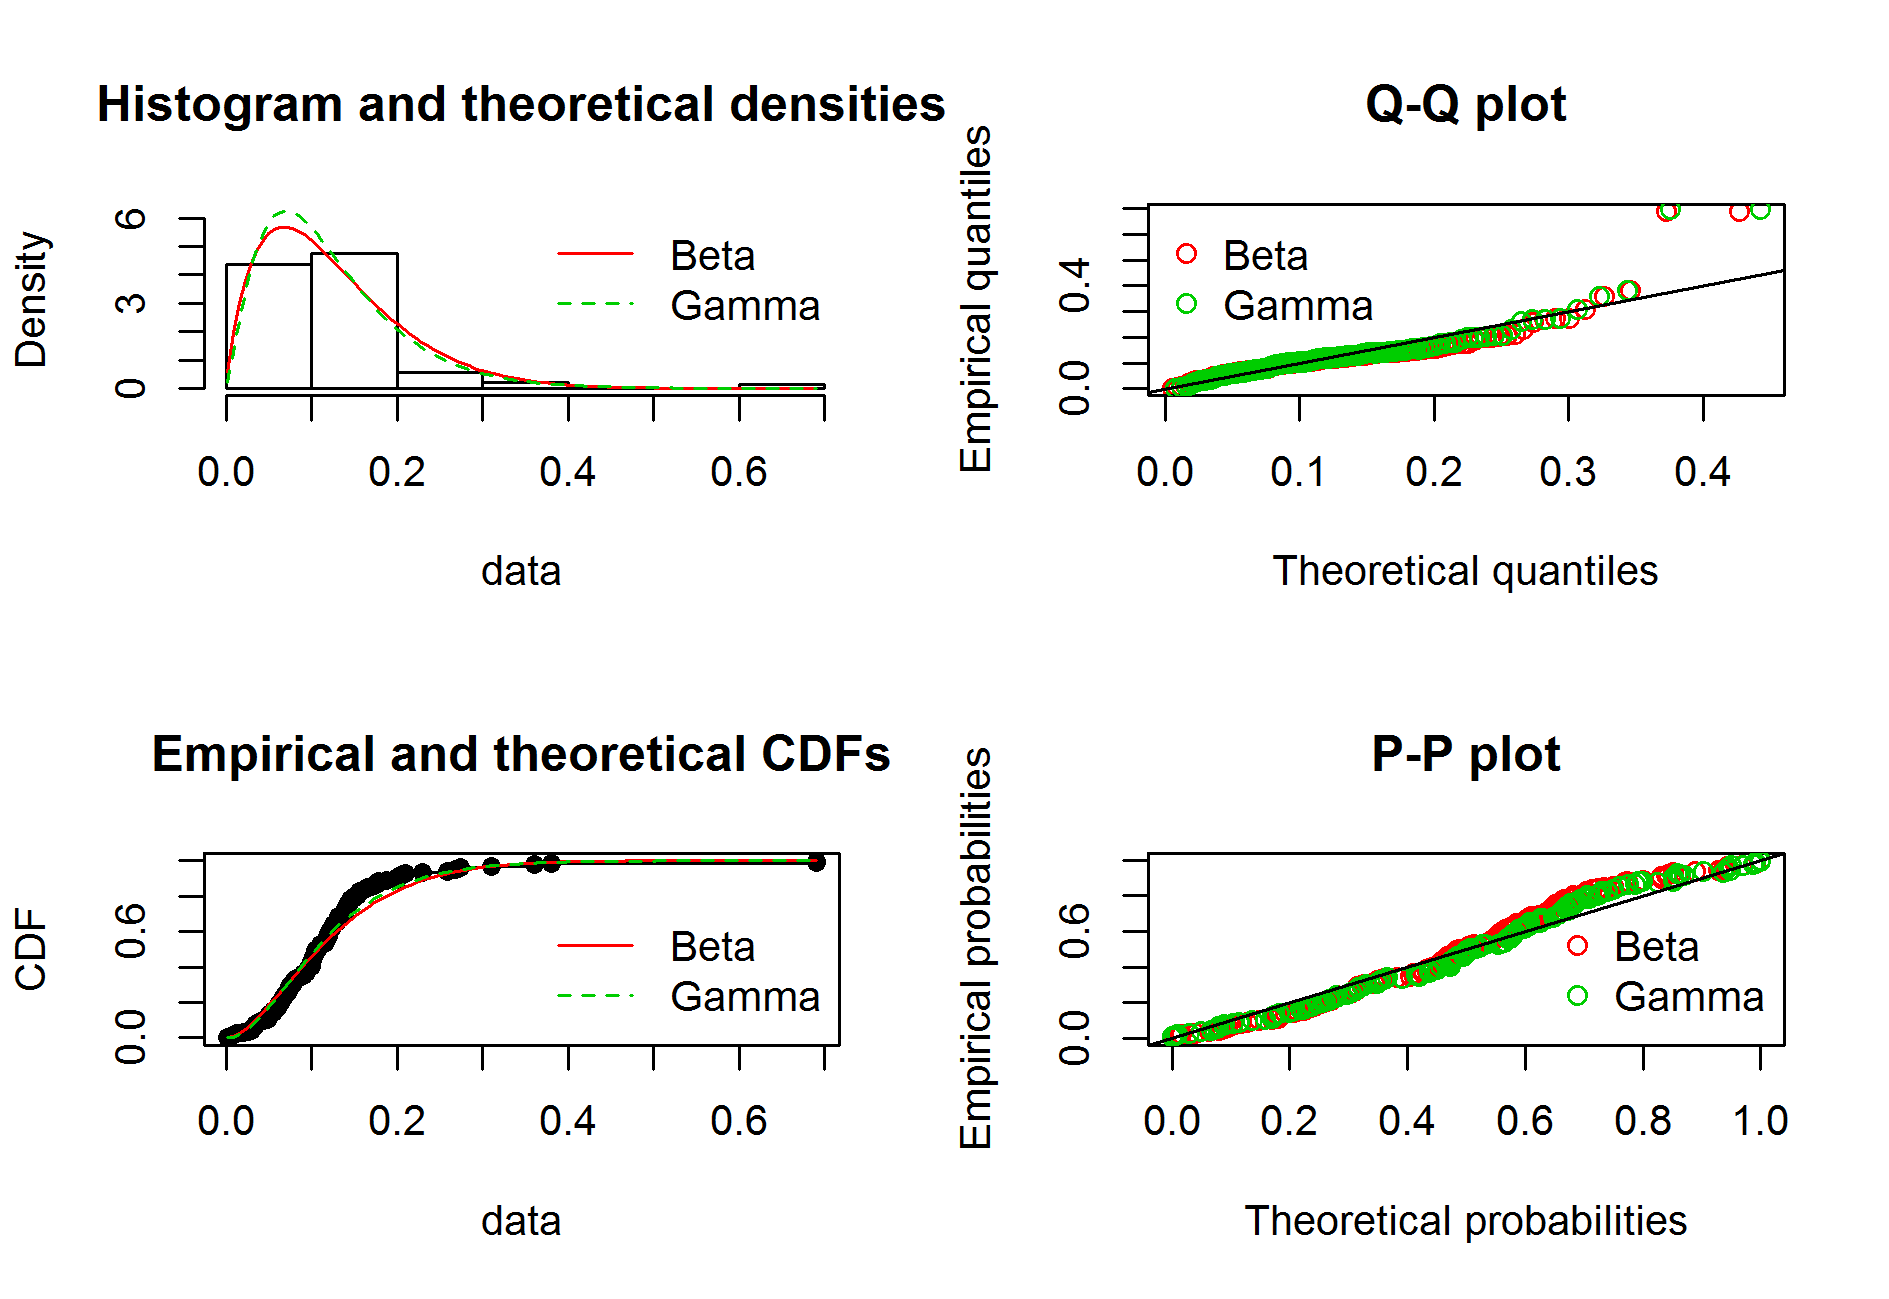
\includegraphics[width=.8\textwidth]{fig/gof_te}
    \caption{Density plots of the fitted distributions to the histogram of the empirical distribution using the marine transfer efficiency data (Case 2), a CDF plot of both the empirical distribution and the fitted distributions (Beta and Gamma), Q-Q plots, and P-P plots. Plot created using R v.3.4.3 \cite{Rcite} fitdistrplus package v.$1.0-9$ \cite{fitdistrplus}. }
    \label{gof_te_a2}
\end{figure}

\begin{table}[H]
\centering
\caption{Goodness-of-fit criteria for transfer efficiency data at trophic level 2}
\begin{tabular}{r|c|c}
  \hline \small
 Goodness-of-fit criteria & Beta  & Gamma \\ 
   \hline
   Akaike's Information Criterion (AIC) & -39.22 & -44.05 \\   
   Bayesian Information Criterion (BIC) & -36.48 &  -41.32  \\
   \hline
\end{tabular} 
\label{te2_aic}
\end{table}

\begin{figure}[H]
     \centering
       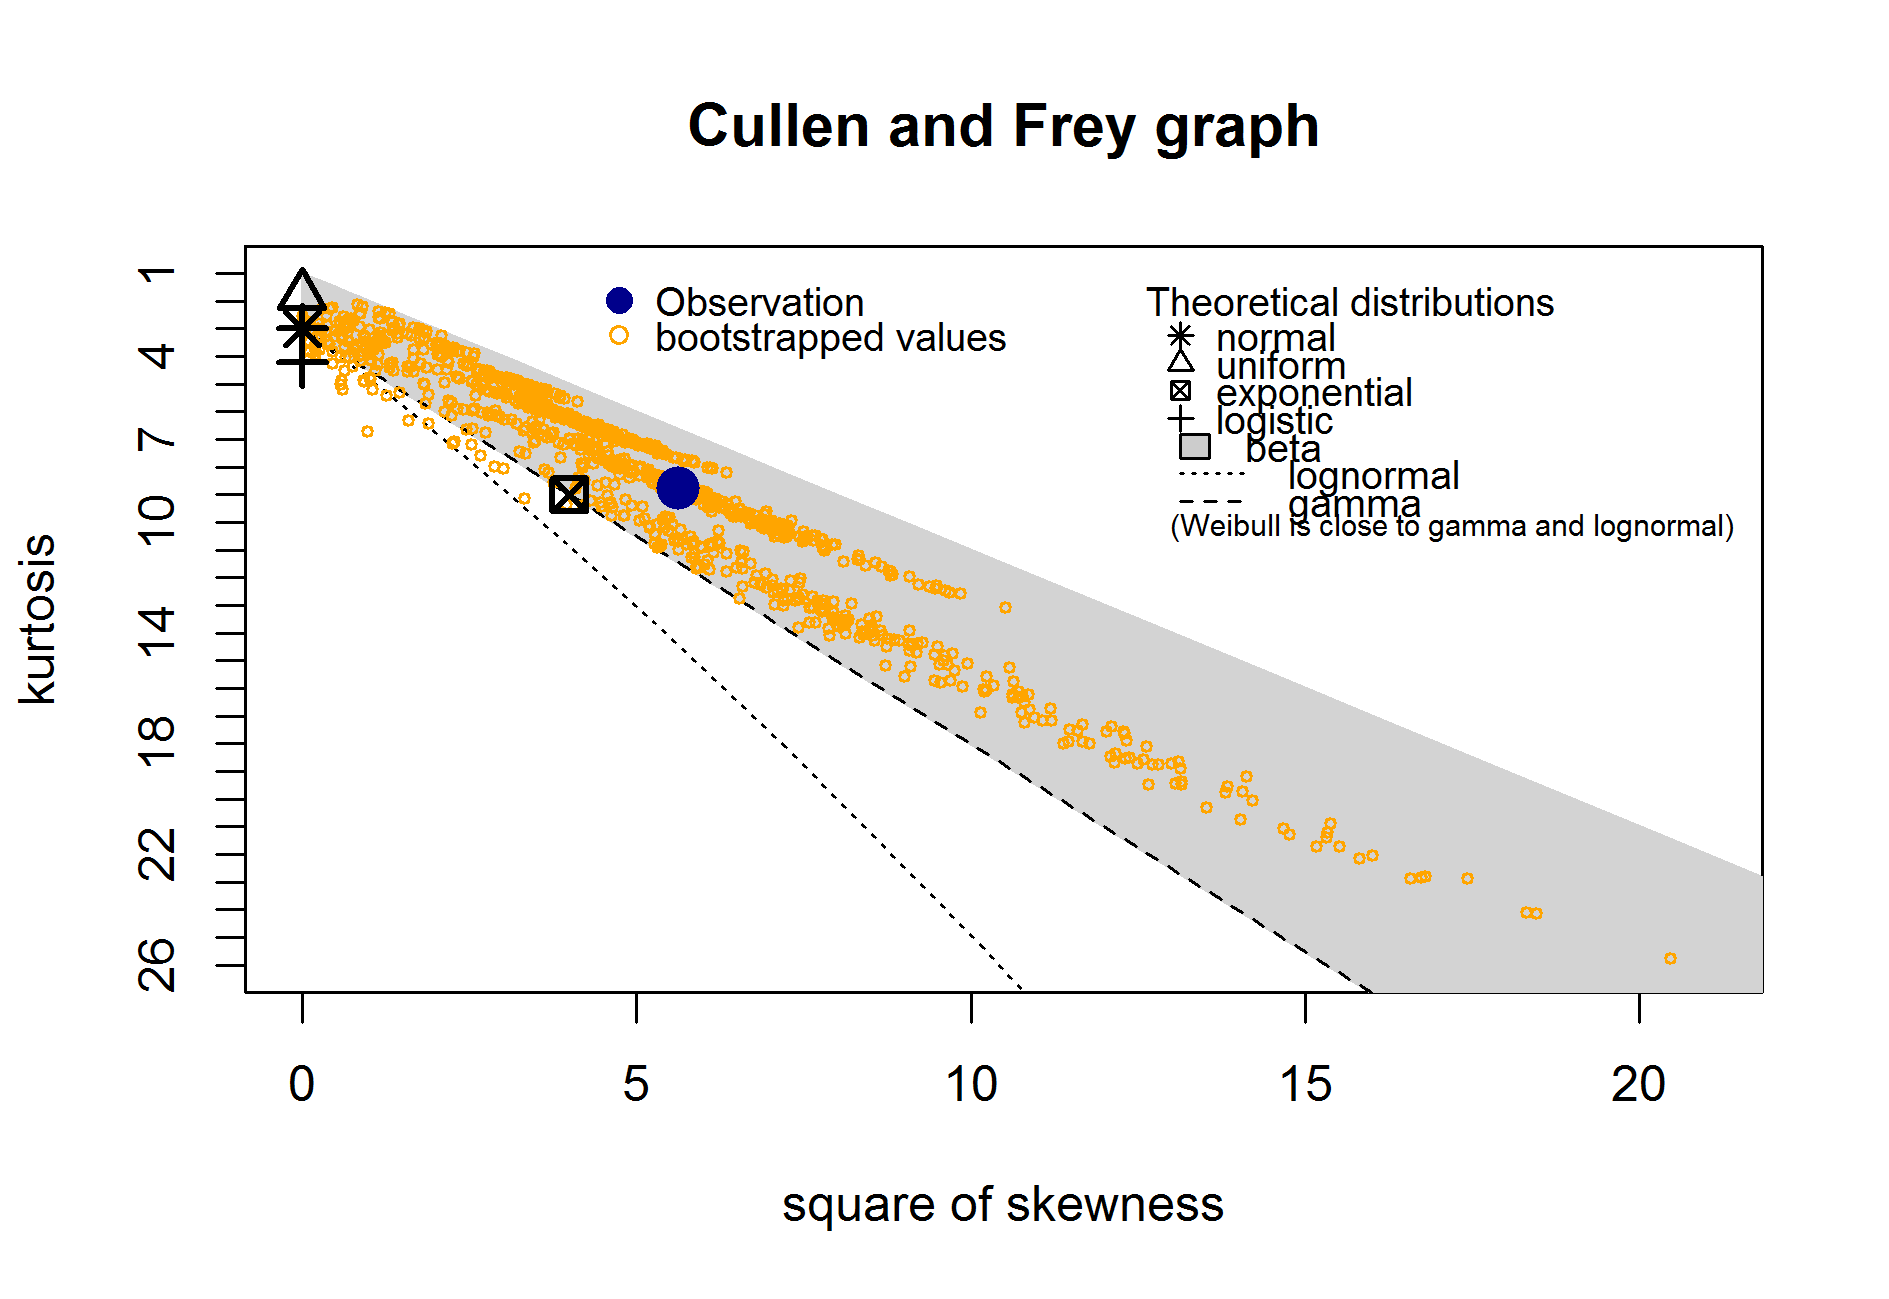
\includegraphics[width=.8\textwidth]{fig/cullen_frey_te2}
    \caption{Visualizes all potential continuous distributions against the marine transfer data for trophic level 2 (Case 3) and bootstrapped data. The figure shows it potentially follows a Beta distribution. Plot created using R v.3.4.3 \cite{Rcite} fitdistrplus package v.$1.0-9$ \cite{fitdistrplus}. }
    \label{cf_te2}
\end{figure}

\begin{figure}[H]
     \centering
       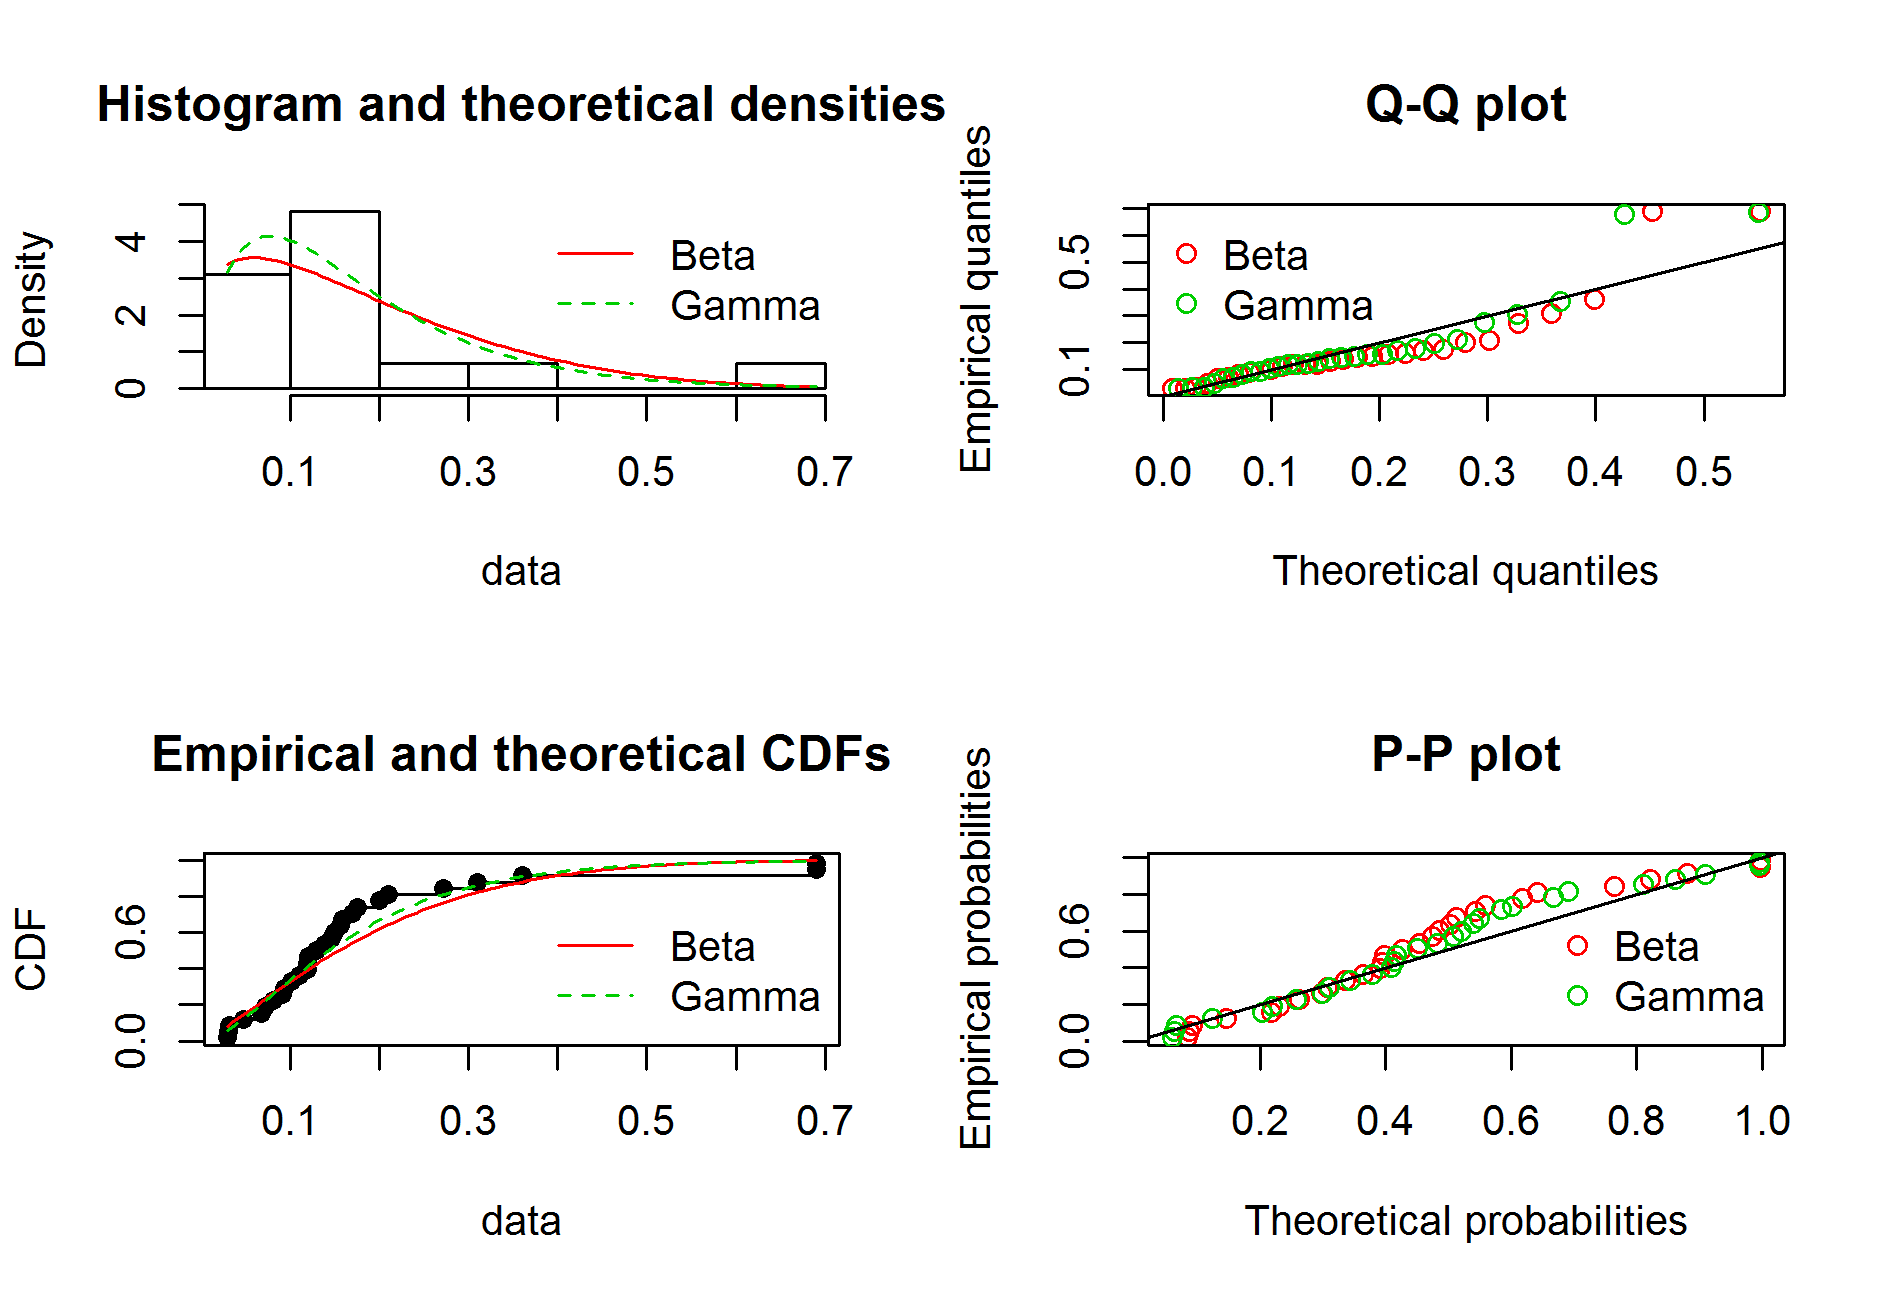
\includegraphics[width=.8\textwidth]{fig/gof_te2}
    \caption{Density plots of the fitted distributions to the histogram of the empirical distribution using the marine transfer efficiency data for trophic level 2 (Case 3), a CDF plot of both the empirical distribution and the fitted distributions (Beta and Gamma), Q-Q plots, and P-P plots. Plot created using R v.3.4.3 \cite{Rcite} fitdistrplus package v.$1.0-9$ \cite{fitdistrplus}. }
    \label{gof_te2}
\end{figure}

\begin{table}[H]
\centering
\caption{Goodness-of-fit criteria for transfer efficiency data at trophic level 3}
\begin{tabular}{r|c|c}
  \hline \small
 Goodness-of-fit criteria & Beta  & Gamma \\ 
   \hline
   Akaike's Information Criterion (AIC) & -25.73 & -25.90 \\   
   Bayesian Information Criterion (BIC) & -24.94 &  -25.11  \\
   \hline
\end{tabular} 
\label{te3_aic}
\end{table}

\begin{figure}[H]
     \centering
       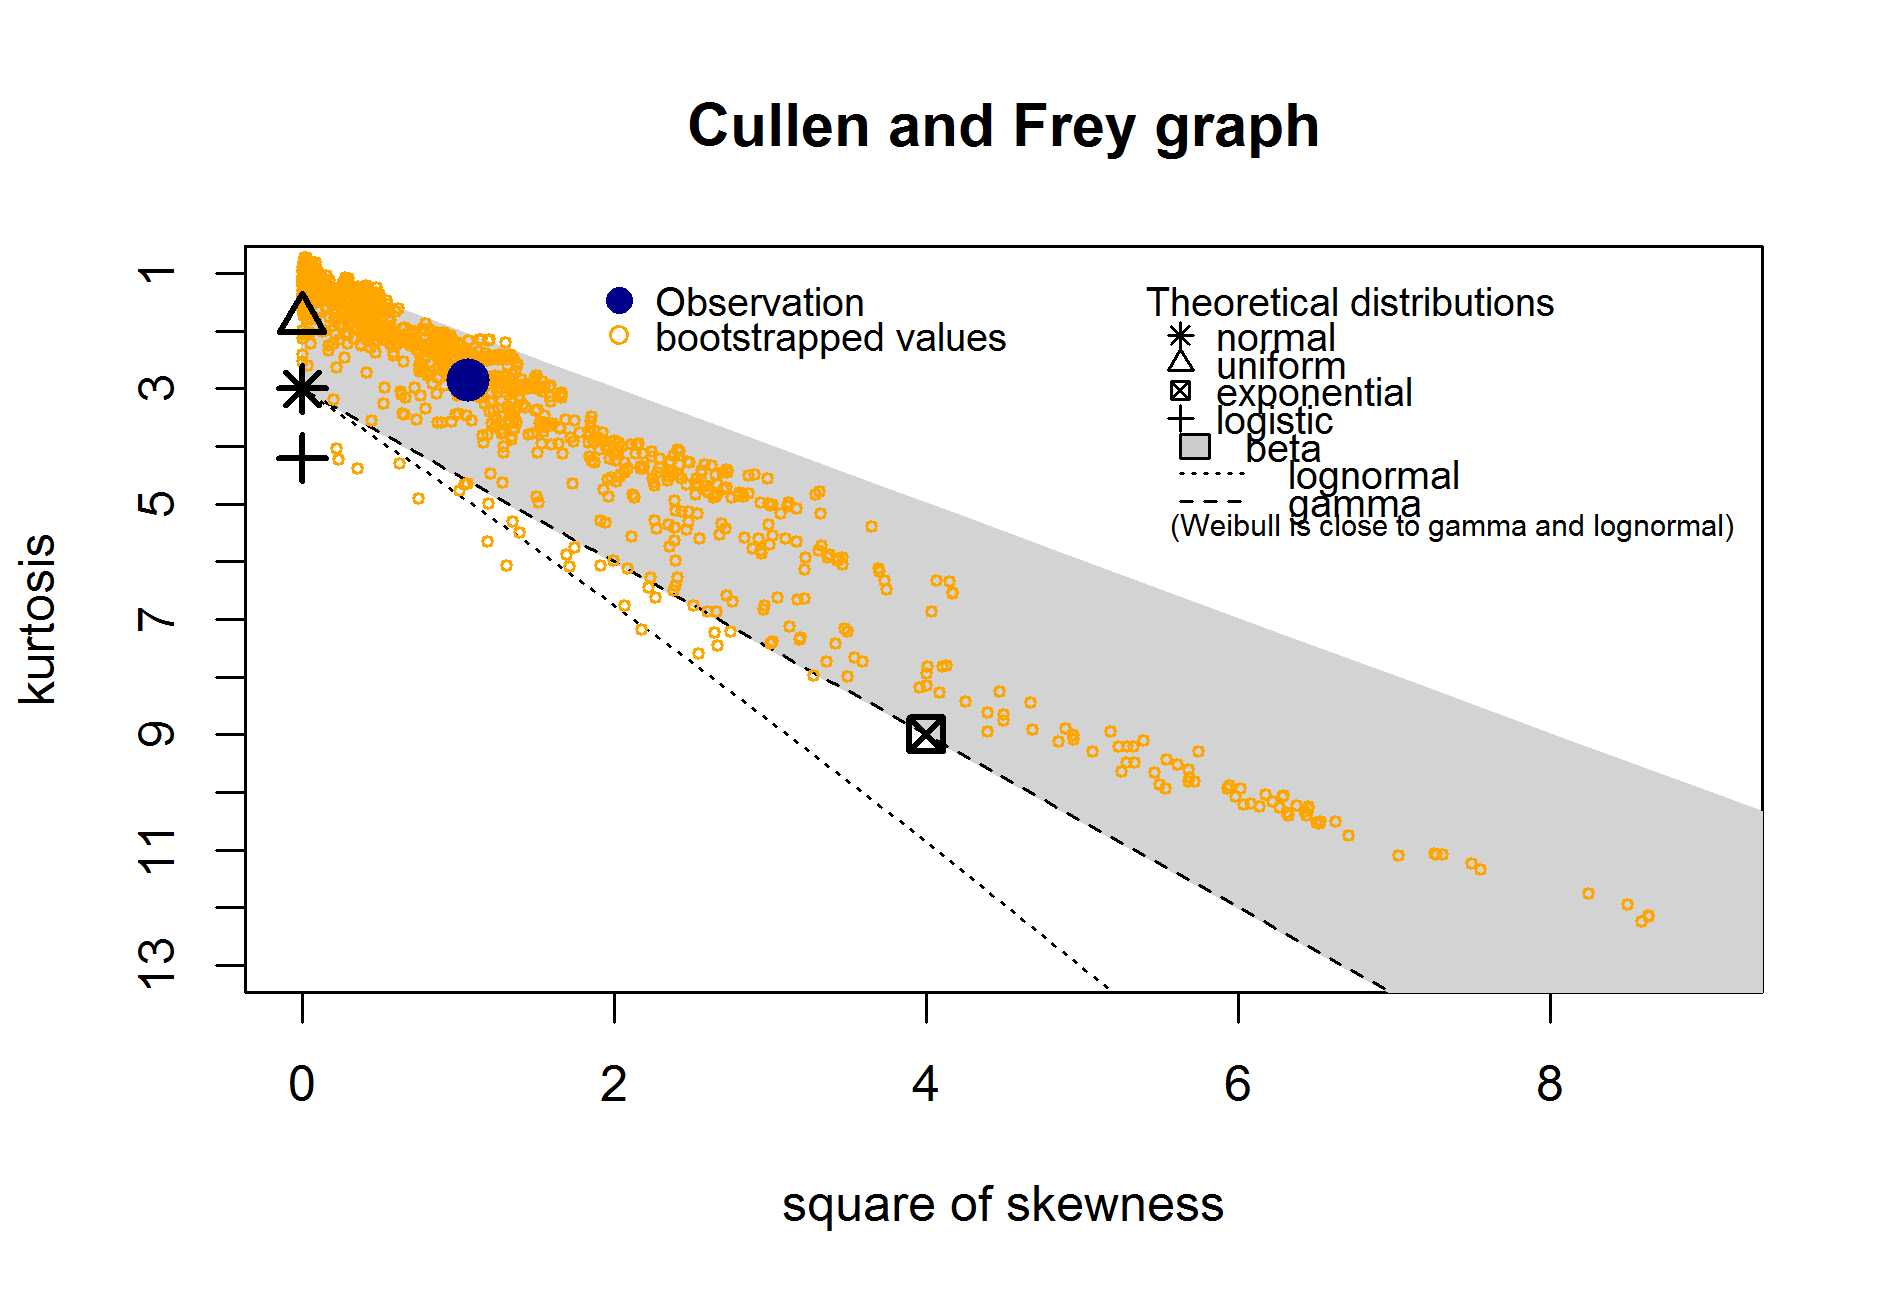
\includegraphics[width=.8\textwidth]{fig/cullen_frey_te3}
    \caption{Visualizes all potential continuous distributions against the marine transfer data for trophic level 3 (Case 3) and bootstrapped data. The figure shows it potentially follows a Beta distribution. Plot created using R v.3.4.3 \cite{Rcite} fitdistrplus package v.$1.0-9$ \cite{fitdistrplus}. }
    \label{cf_te3}
\end{figure}

\begin{figure}[H]
     \centering
       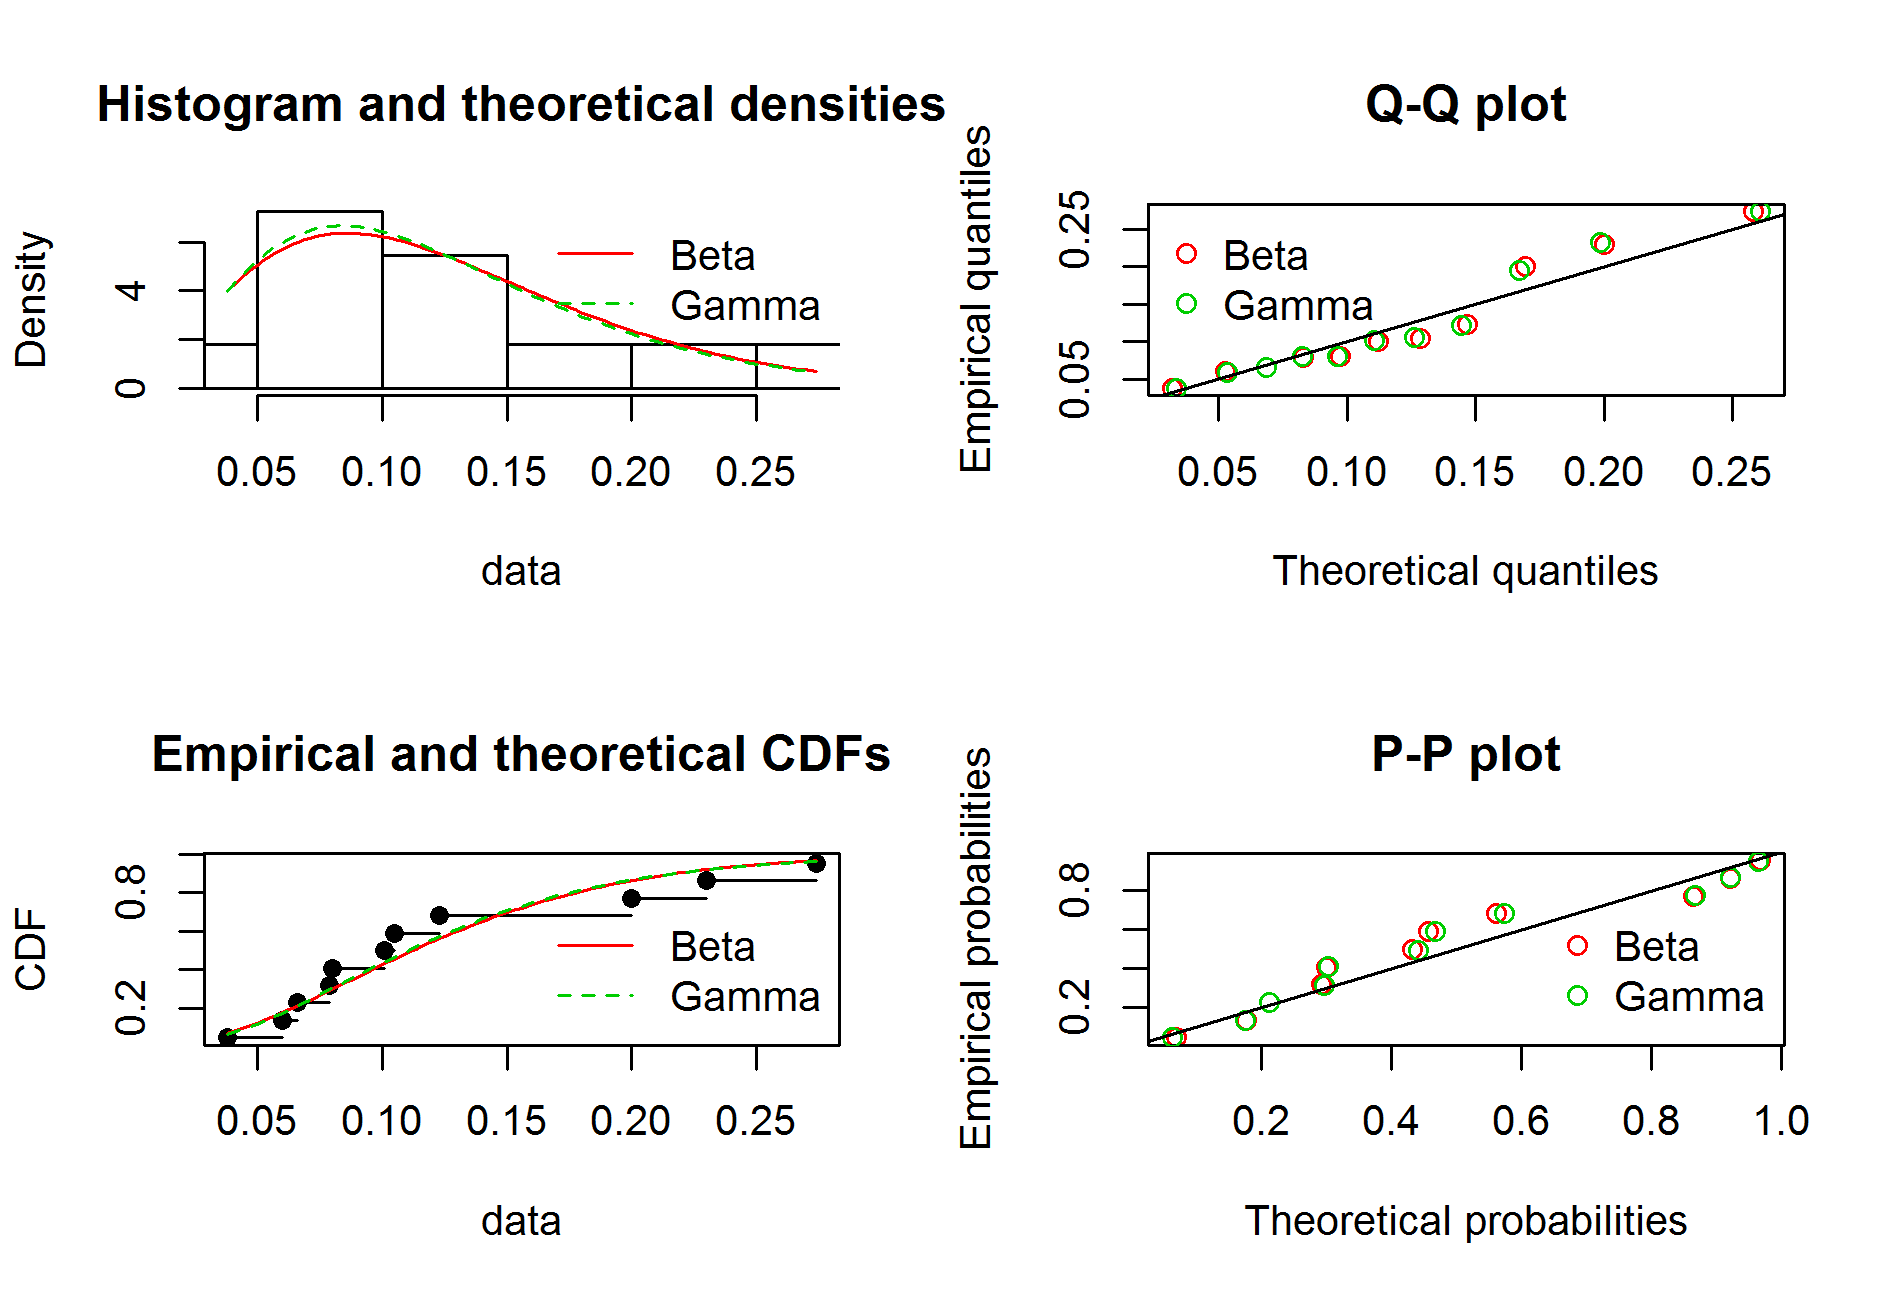
\includegraphics[width=.8\textwidth]{fig/gof_te3}
    \caption{Density plots of the fitted distributions to the histogram of the empirical distribution using the marine transfer efficiency data for trophic level 3 (Case 3), a CDF plot of both the empirical distribution and the fitted distributions (Beta and Gamma), Q-Q plots, and P-P plots. Plot created using R v.3.4.3 \cite{Rcite} fitdistrplus package v.$1.0-9$ \cite{fitdistrplus}. }
    \label{gof_te3}
\end{figure}

\begin{table}[H]
\centering
\caption{Goodness-of-fit criteria for transfer efficiency data at trophic level 4}
\begin{tabular}{r|c|c}
  \hline \small
 Goodness-of-fit criteria & Beta  & Gamma \\ 
   \hline
   Akaike's Information Criterion (AIC) & -9.54 & -10.32 \\   
   Bayesian Information Criterion (BIC) & -9.73 &  -10.51  \\
   \hline
\end{tabular} 
\label{te4_aic}
\end{table}

\begin{figure}[H]
     \centering
       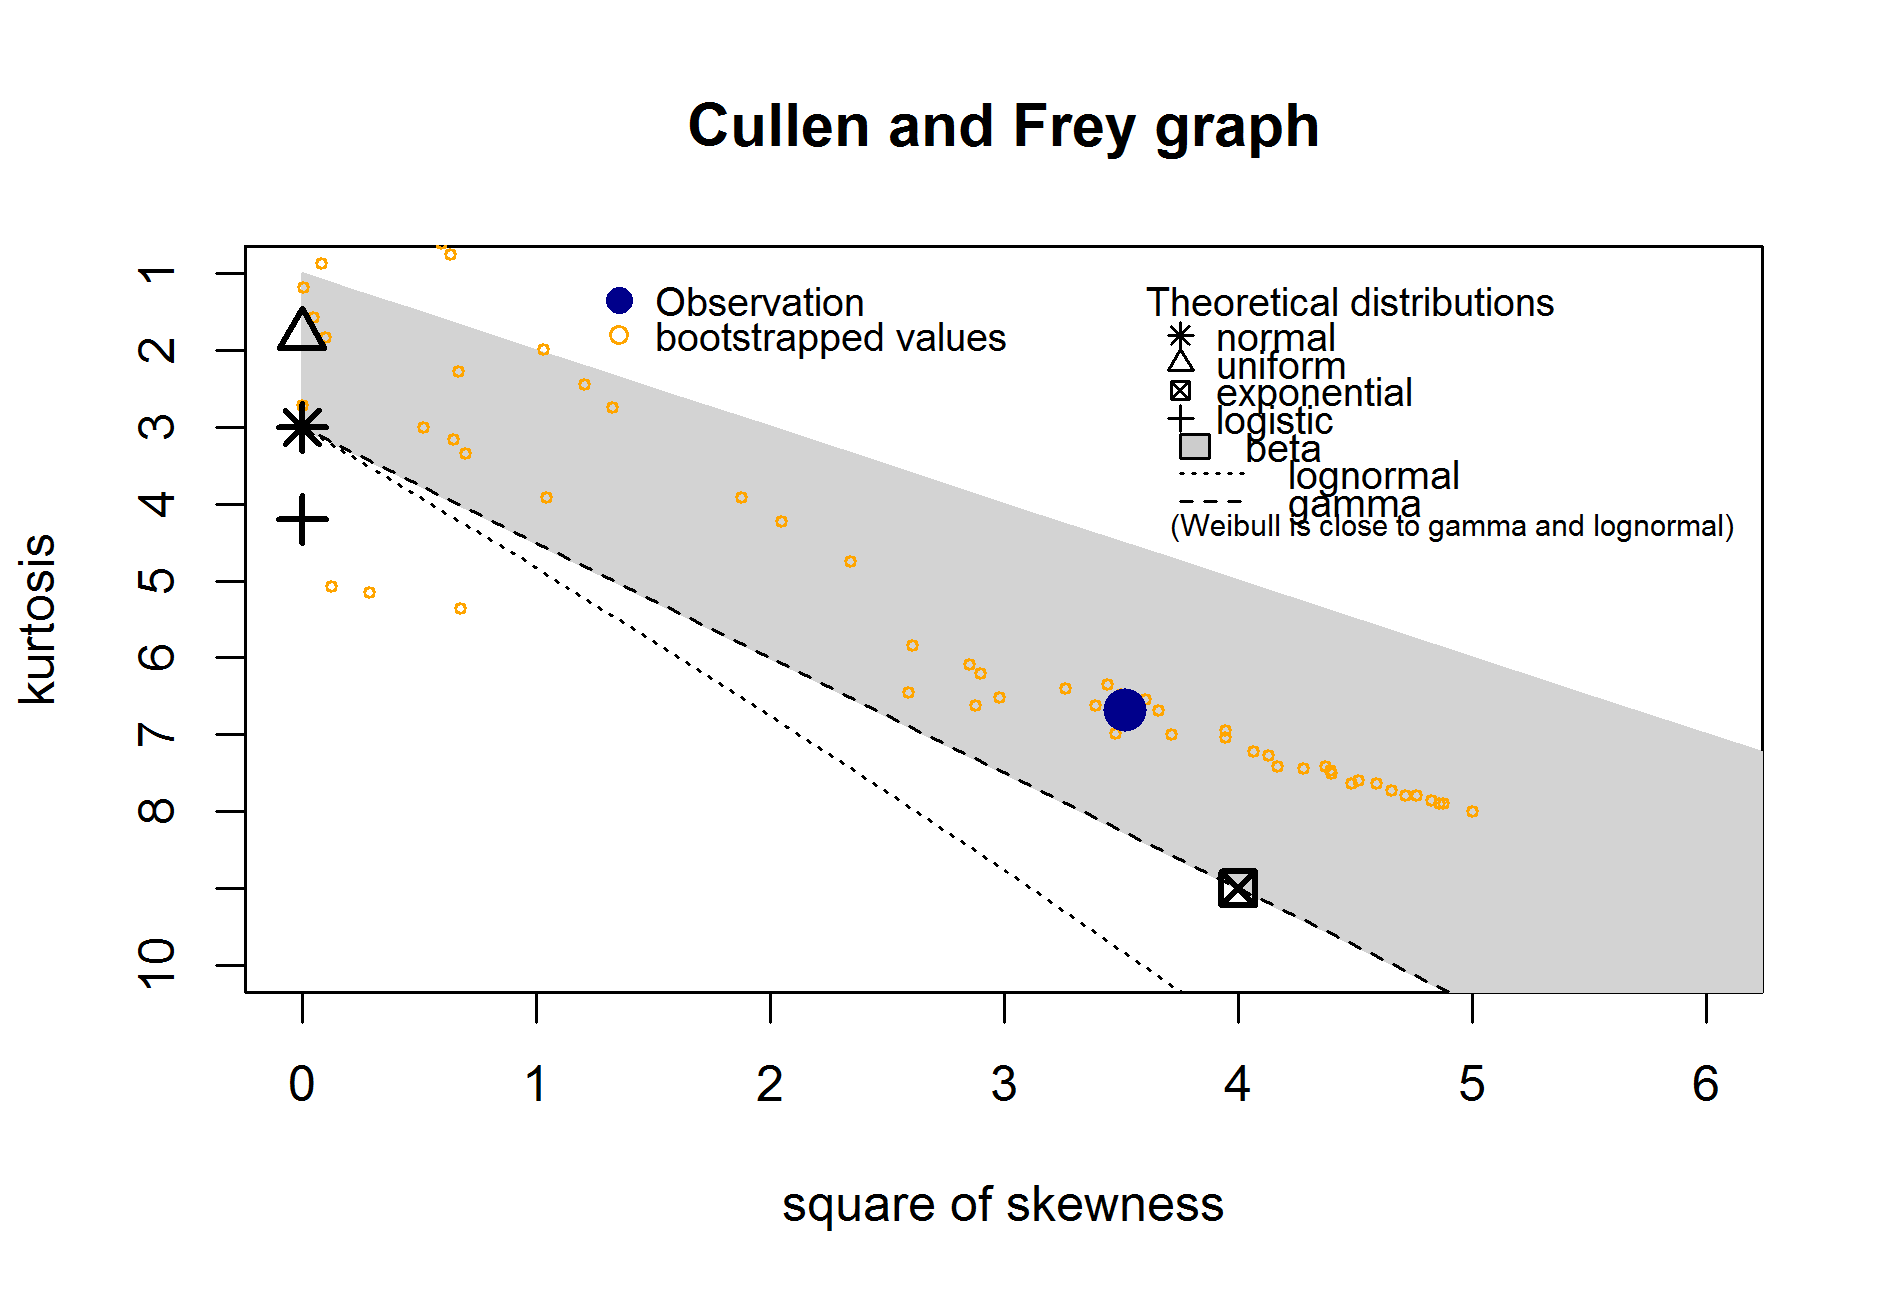
\includegraphics[width=.8\textwidth]{fig/cullen_frey_te4}
    \caption{Visualizes all potential continuous distributions against the marine transfer data for trophic level 4 (Case 3) and bootstrapped data. The figure shows it potentially follows a Beta distribution. Plot created using R v.3.4.3 \cite{Rcite} fitdistrplus package v.$1.0-9$ \cite{fitdistrplus}. }
    \label{cf_te4}
\end{figure}

\begin{figure}[H]
     \centering
       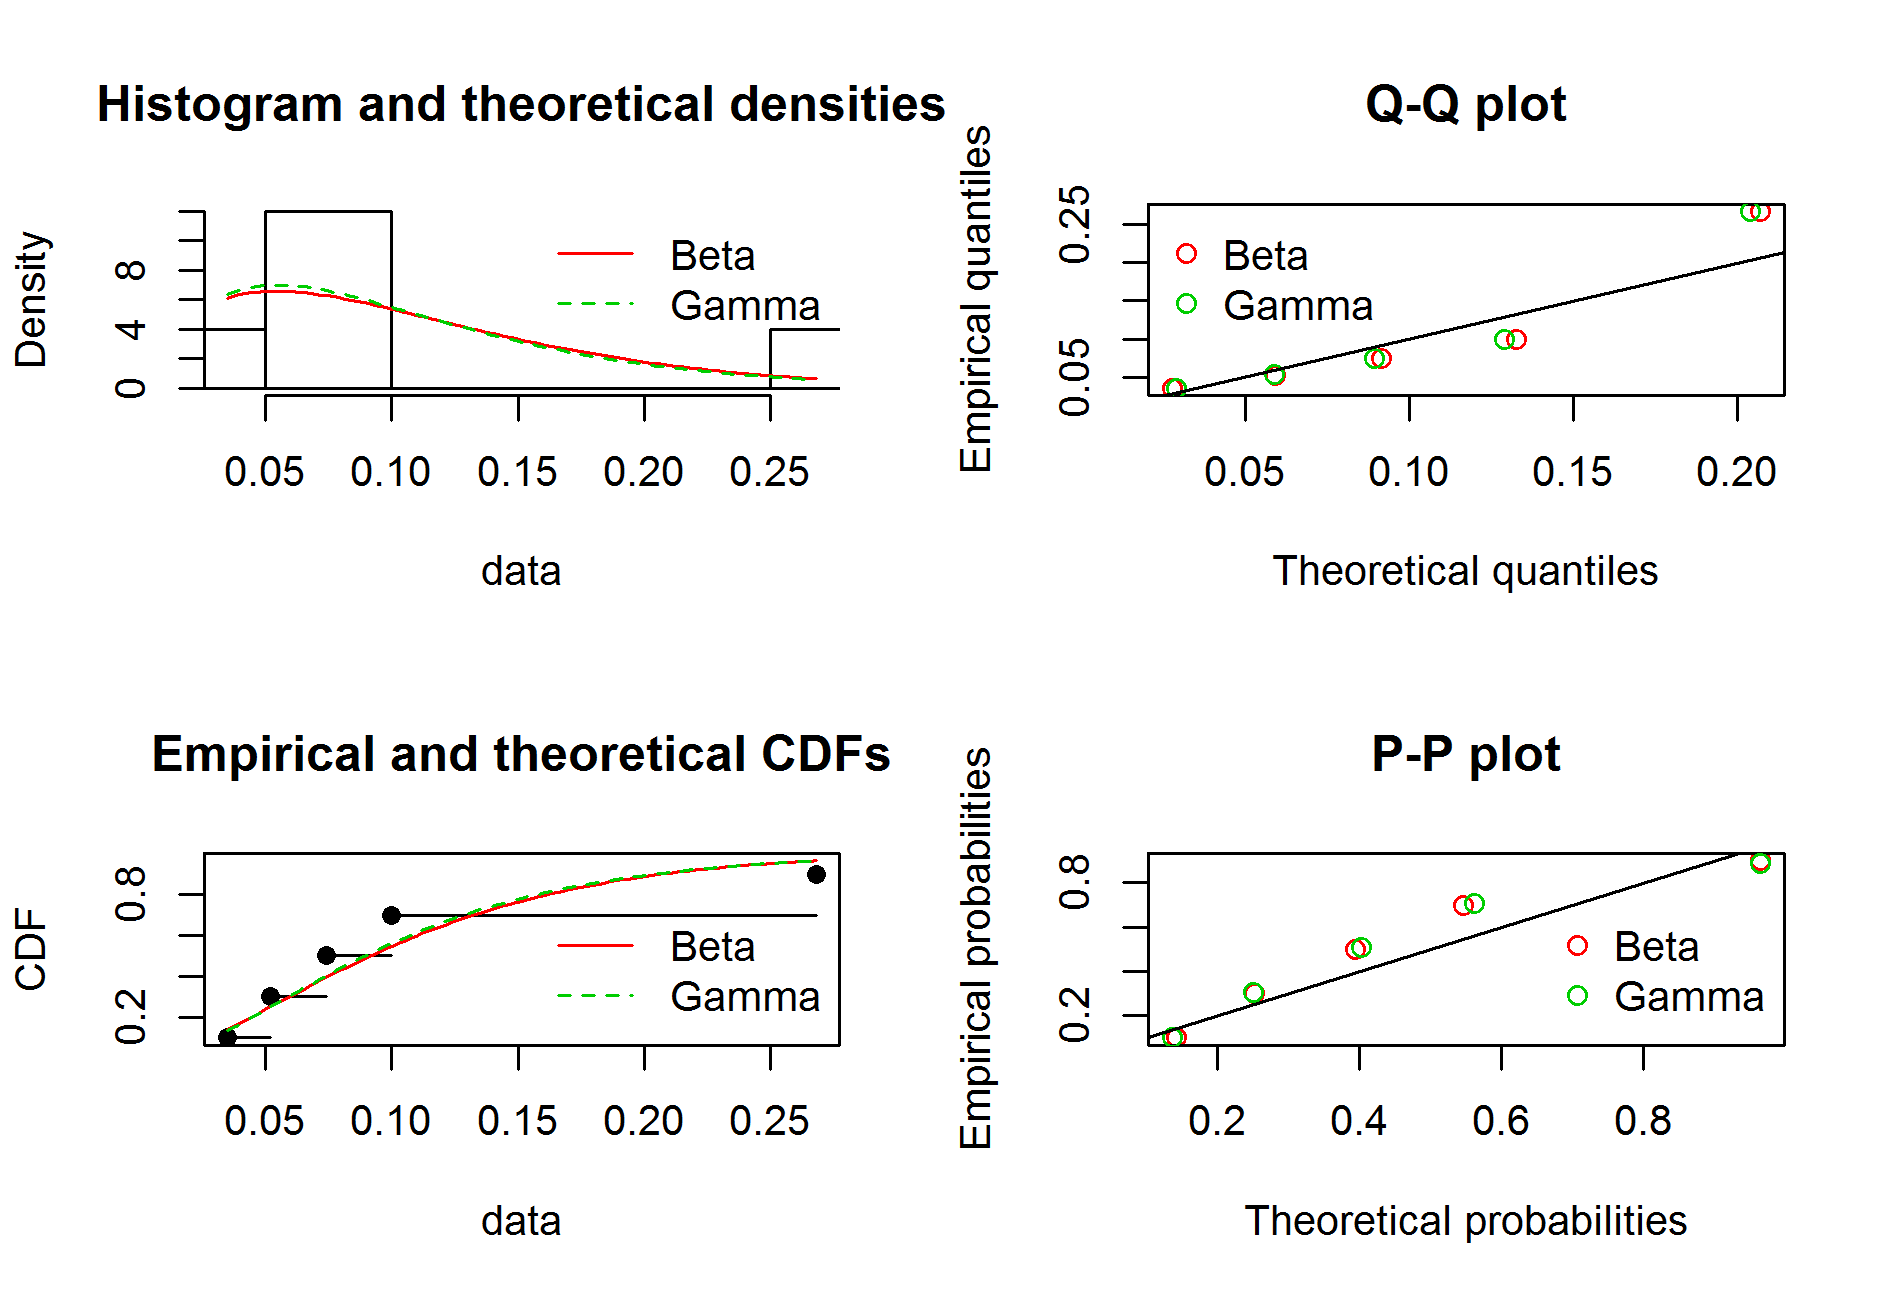
\includegraphics[width=.8\textwidth]{fig/gof_te4}
    \caption{Density plots of the fitted distributions to the histogram of the empirical distribution using the marine transfer efficiency data for trophic level 4 (Case 3), a CDF plot of both the empirical distribution and the fitted distributions (Beta and Gamma), Q-Q plots, and P-P plots. Plot created using R v.3.4.3 \cite{Rcite} fitdistrplus package v.$1.0-9$ \cite{fitdistrplus}. }
    \label{gof_te4}
\end{figure}

\subsection{FishBase}
\subsubsection{Trophic Level}
Estimated trophic levels (rational numbers) were calculated from the FishBase database (\url{http://www.fishbase.org/}) for each species and truncated to cluster species into integer-valued trophic levels. Truncated trophic levels range in the MHI from $h=1,\dots,4$ with $h=1$ representing phytoplankton, $h=2$ primary consumers, $h=3$ secondary consumers, and $h=4$ tertiary consumers. If the rational number was greater than or equal to 4, then the organism was put into trophic level 4, if it was less than 4 and greater than or equal to 3 it was put into trophic level 3, and if it was less than 3 it was put into trophic level 2. The number of species found at each trophic level were not equal.

\subsubsection{Maximum Expected Lifespan}
The maximum expected lifespan $\lambda_h$ for species at trophic level $h = 2, 3, 4$ was treated as a random value in Case 2. We ran goodness-of-fit tests for each level of $h$ to find an approximate distribution. We started off with a skewness-kurtosis plot (Fig. \ref{cf_l2}, \ref{cf_l3}, and \ref{cf_l4}) to initially decide which distributions to consider (i.e., Lognormal, Weibull, and Gamma) \cite{fitdistrplus}. Then we fitted individual distributions to the data using maximum likelihood estimation and compared density plots of the fitted distributions to the histogram of the empirical distribution, a cumulative distribution (CDF) plot of both the empirical distribution and the fitted distributions, Q-Q plots, and P-P plots (Fig. \ref{gof_l2}, \ref{gof_l3}, and \ref{gof_l4}). Lastly, we used AIC and BIC criterion to choose the most approximate distribution (Table \ref{l2_aic}, \ref{l3_aic}, and \ref{l4_aic}). We found for all trophic levels the most appropriate approximate distribution was a Lognormal distribution, where each trophic level has distinct values for $\mu$ and $\sigma^2$. 

\begin{table}[H]
\centering
\caption{Goodness-of-fit criteria for maximum expected lifespan data at trophic level 2}
\begin{tabular}{r|c|c|c}
  \hline \small
 Goodness-of-fit criteria & Lognormal & Weibell & Gamma \\ 
   \hline
   Akaike's Information Criterion (AIC) & 558.43 & 580.58 & 571.93 \\   
   Bayesian Information Criterion (BIC) & 563.55 & 585.71 & 577.06 \\
   \hline
\end{tabular} 
\label{l2_aic}
\end{table}

\begin{figure}[H]
     \centering
       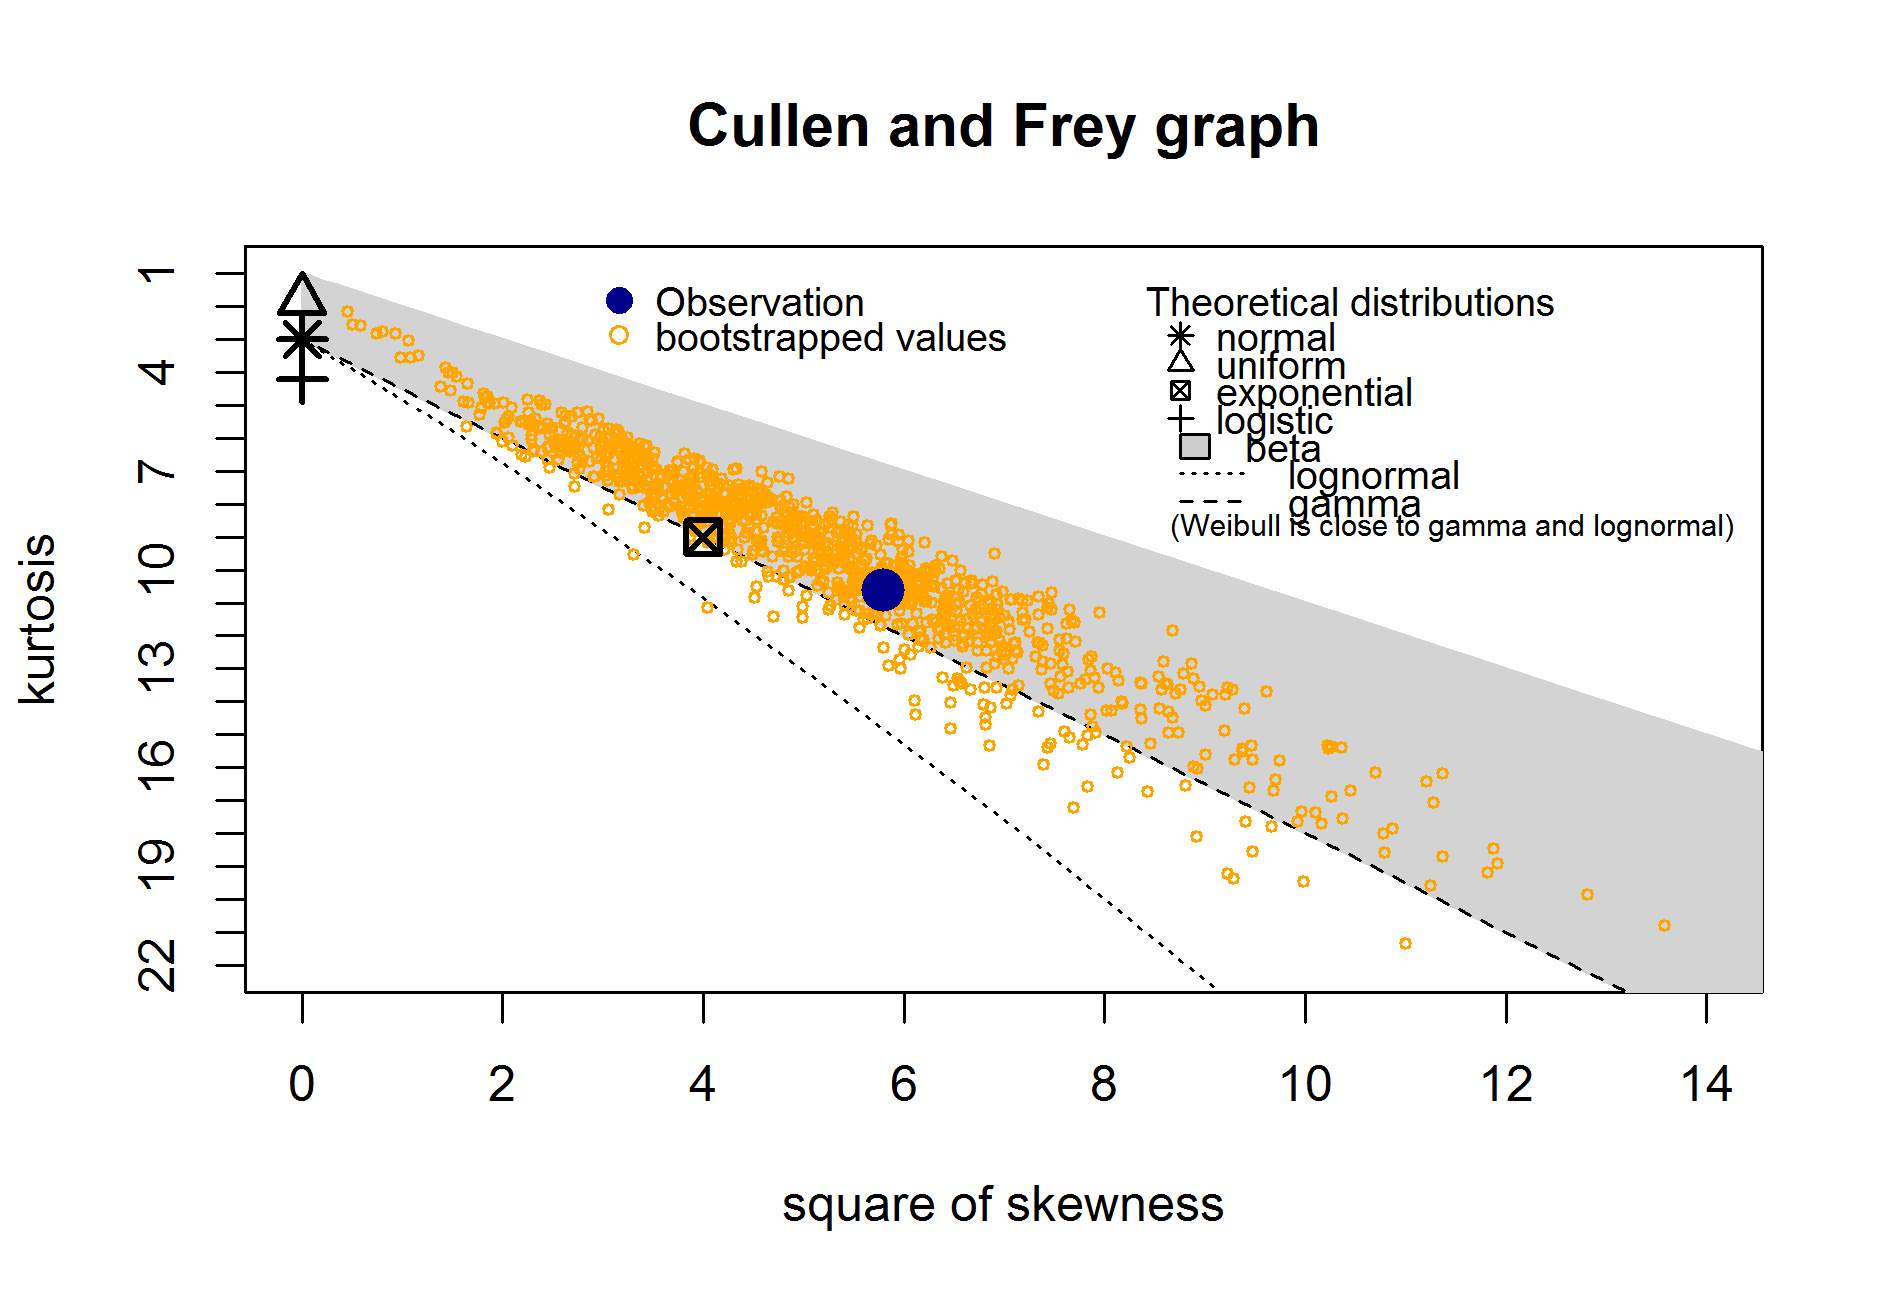
\includegraphics[width=.8\textwidth]{fig/cullen_frey_l2}
    \caption{Visualizes all potential continuous distributions against the maximum expected lifespan data for trophic level 2 and bootstrapped data. The figure shows it potentially follows a Gamma, Weibull, and Lognormal distribution. Plot created using R v.3.4.3 \cite{Rcite} fitdistrplus package v.$1.0-9$ \cite{fitdistrplus}. }
    \label{cf_l2}
\end{figure}

\begin{figure}[H]
     \centering
       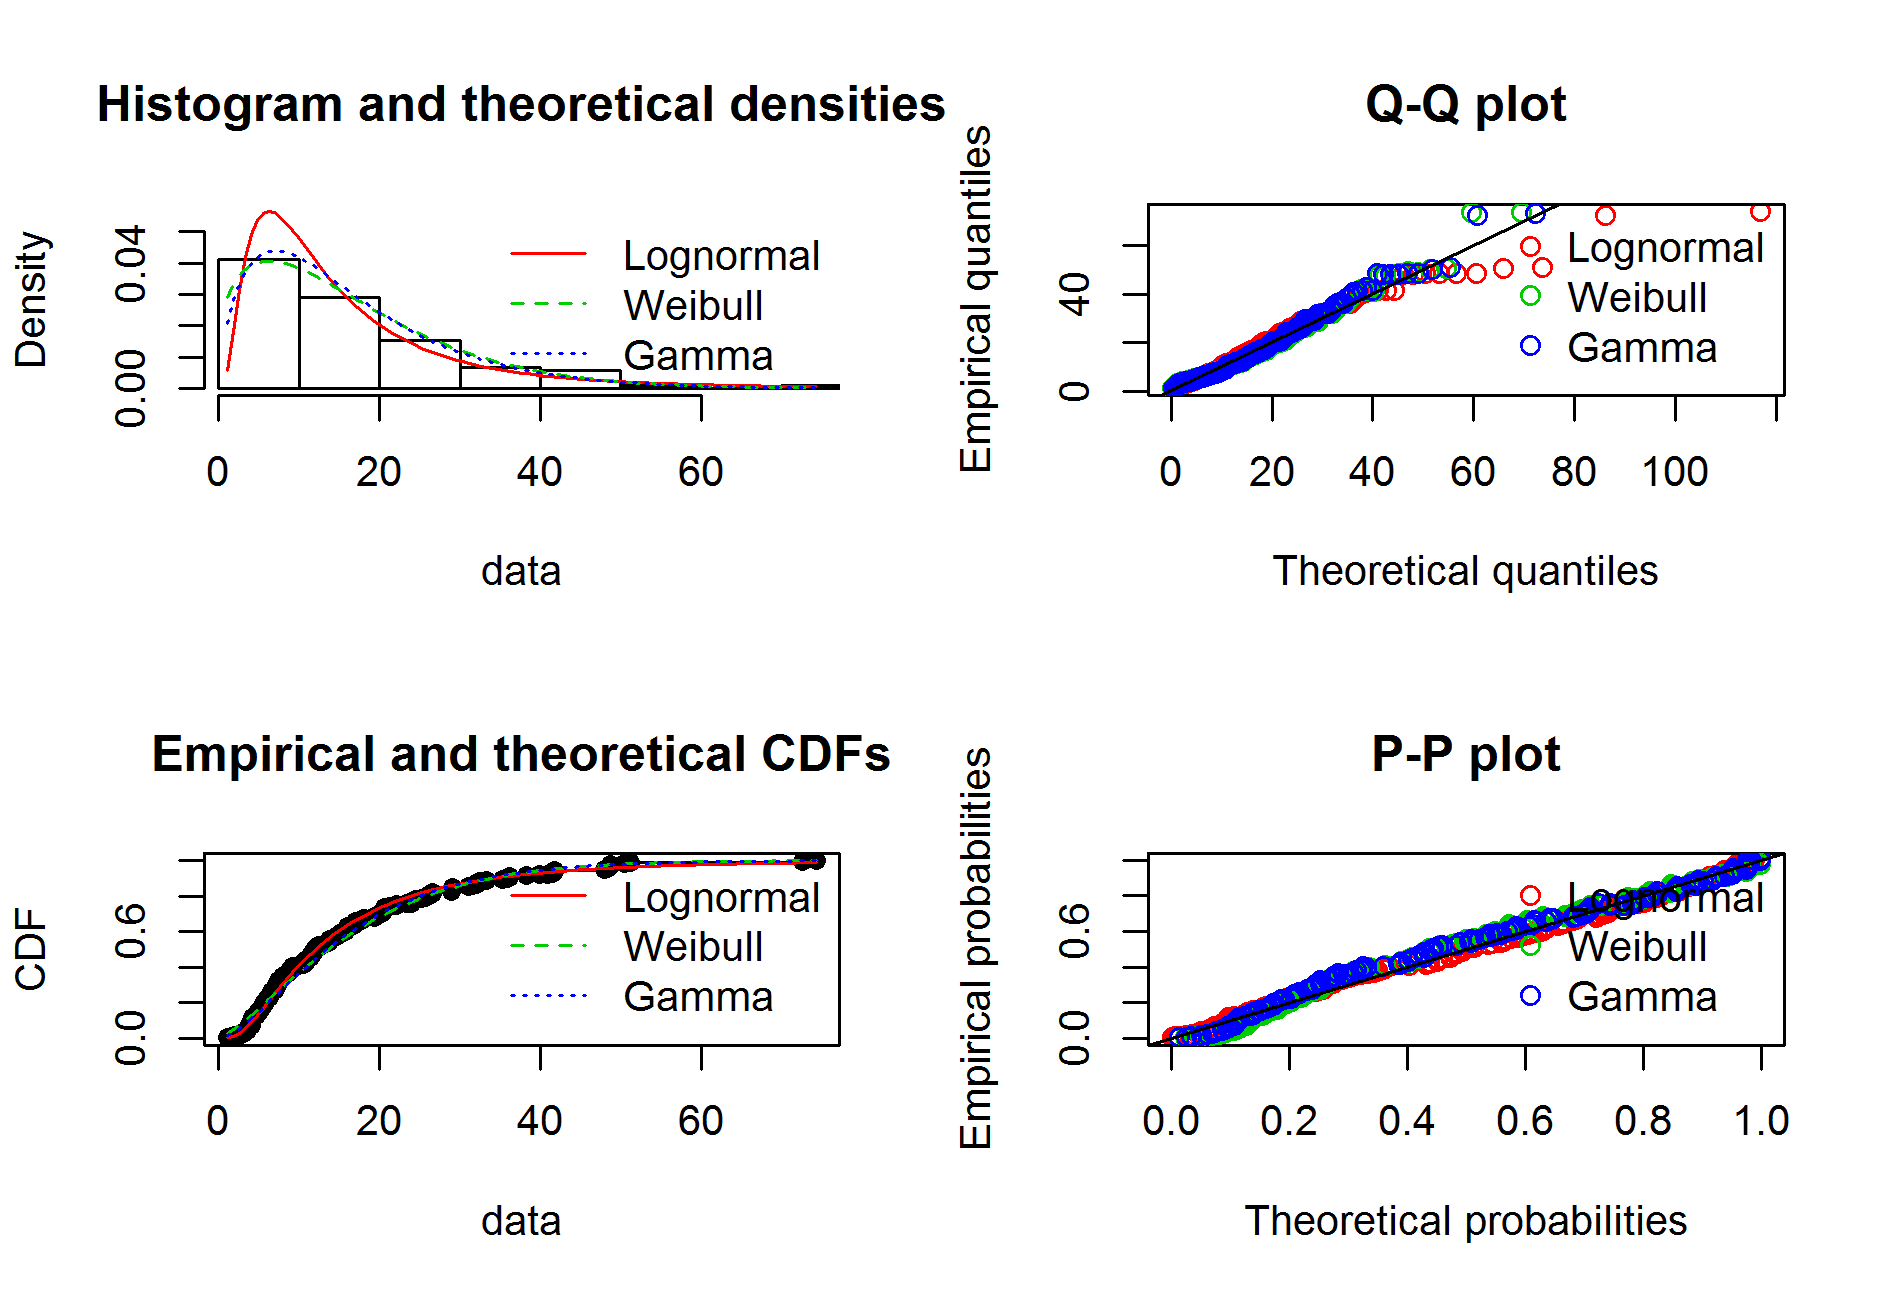
\includegraphics[width=.8\textwidth]{fig/gof_l2}
    \caption{Density plots of the fitted distributions to the histogram of the empirical distribution using the maximum expected lifespan data for trophic level 2, a CDF plot of both the empirical distribution and the fitted distributions (Gamma, Weibull, and Lognormal), Q-Q plots, and P-P plots. Plot created using R v.3.4.3 \cite{Rcite} fitdistrplus package v.$1.0-9$ \cite{fitdistrplus}. }
    \label{gof_l2}
\end{figure}

\begin{table}[H]
\centering
\caption{Goodness-of-fit criteria for maximum expected lifespan data at trophic level 3}
\begin{tabular}{r|c|c|c}
  \hline \small
 Goodness-of-fit criteria & Lognormal & Weibell & Gamma \\ 
   \hline
   Akaike's Information Criterion (AIC) & 1980.06 & 2030.41 & 2011.78 \\   
   Bayesian Information Criterion (BIC) & 1987.66 & 2038.01 & 2019.38 \\
   \hline
\end{tabular} 
\label{l3_aic}
\end{table}

\begin{figure}[H]
     \centering
       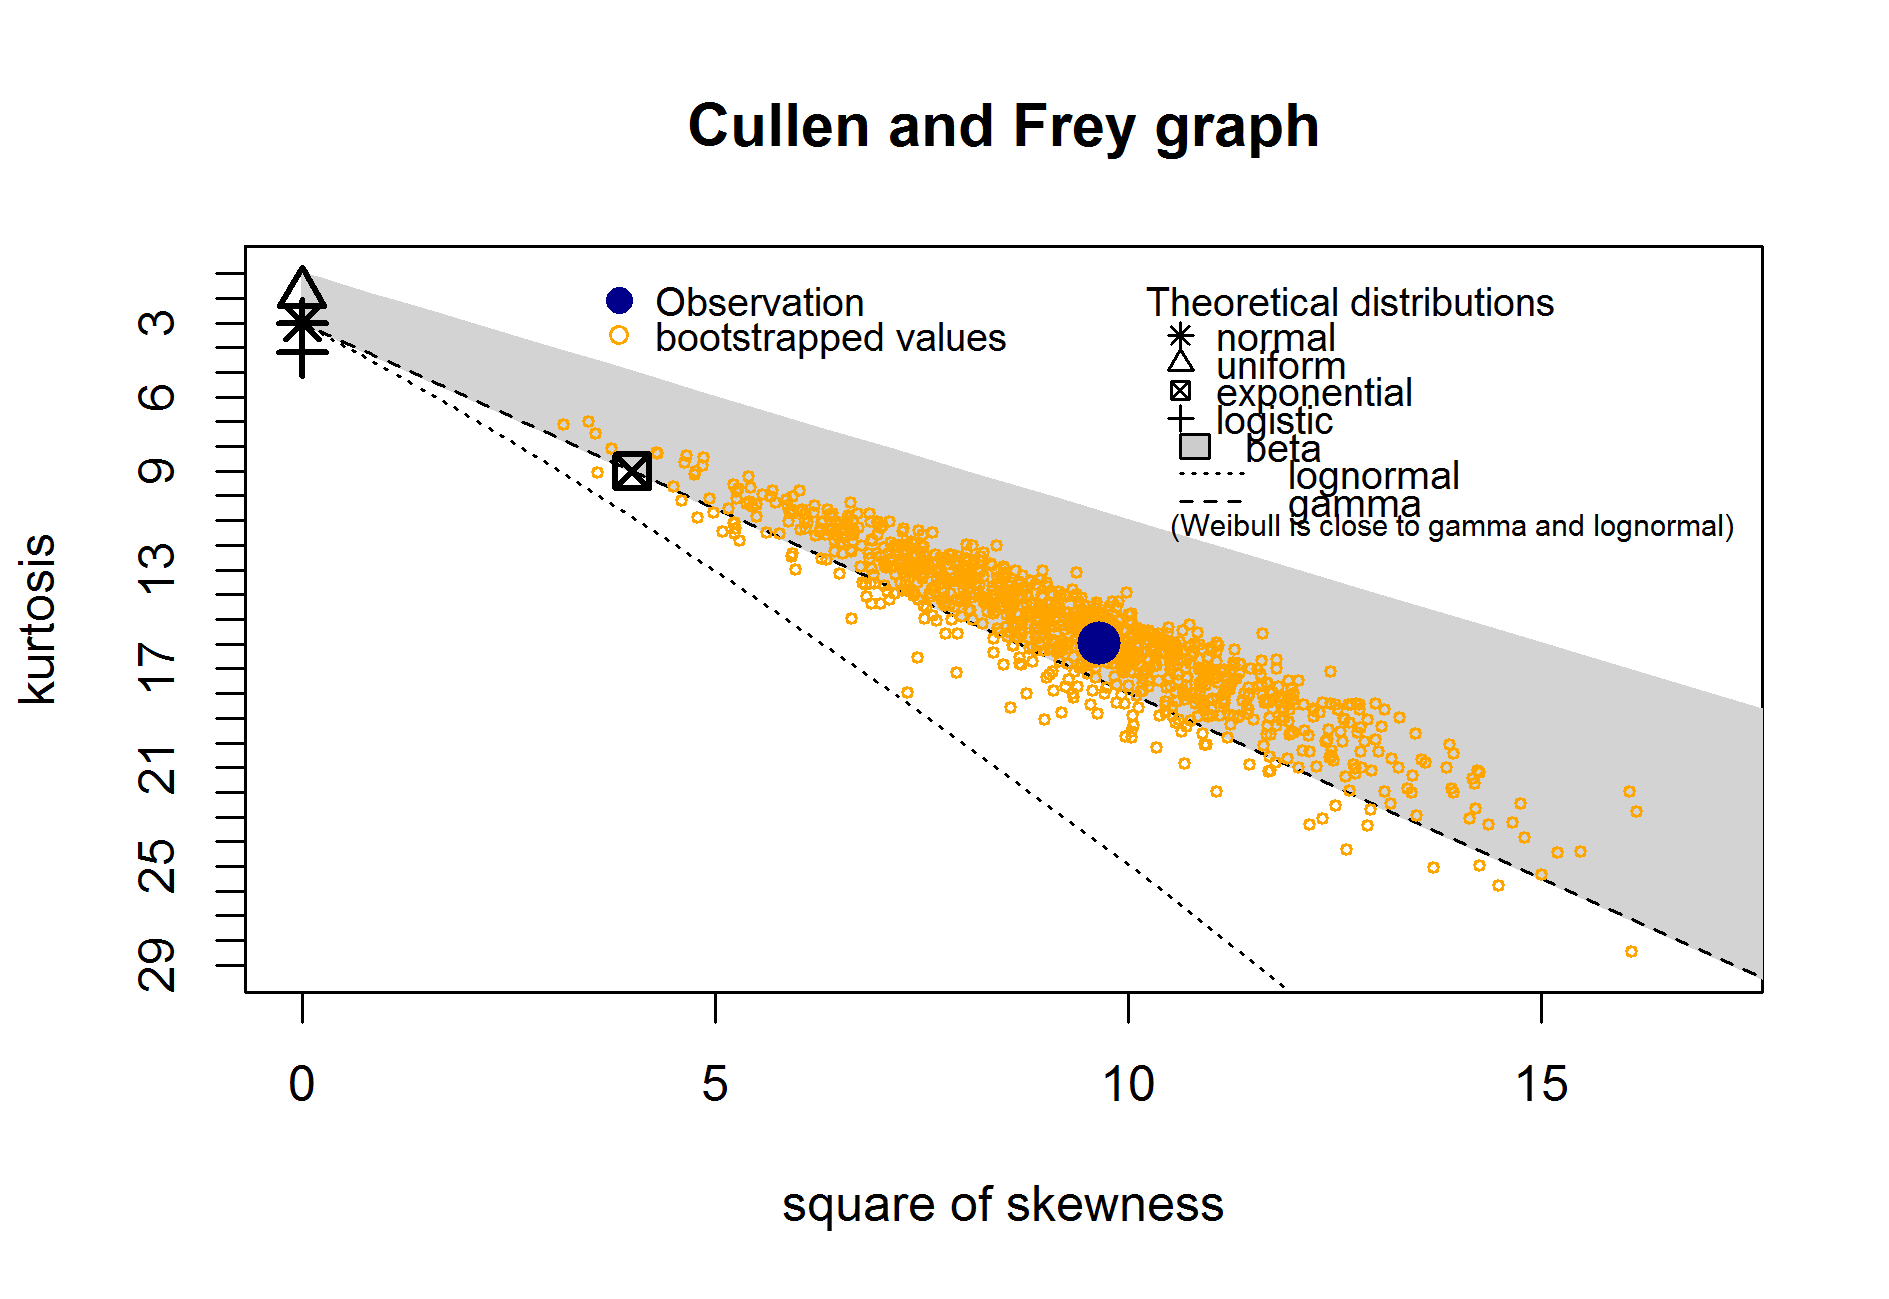
\includegraphics[width=.8\textwidth]{fig/cullen_frey_l3}
    \caption{Visualizes all potential continuous distributions against the maximum expected lifespan data for trophic level 3 and bootstrapped data. The figure shows it potentially follows a Gamma, Weibull, and Lognormal distribution. Plot created using R v.3.4.3 \cite{Rcite} fitdistrplus package v.$1.0-9$ \cite{fitdistrplus}. }
    \label{cf_l3}
\end{figure}

\begin{figure}[H]
     \centering
       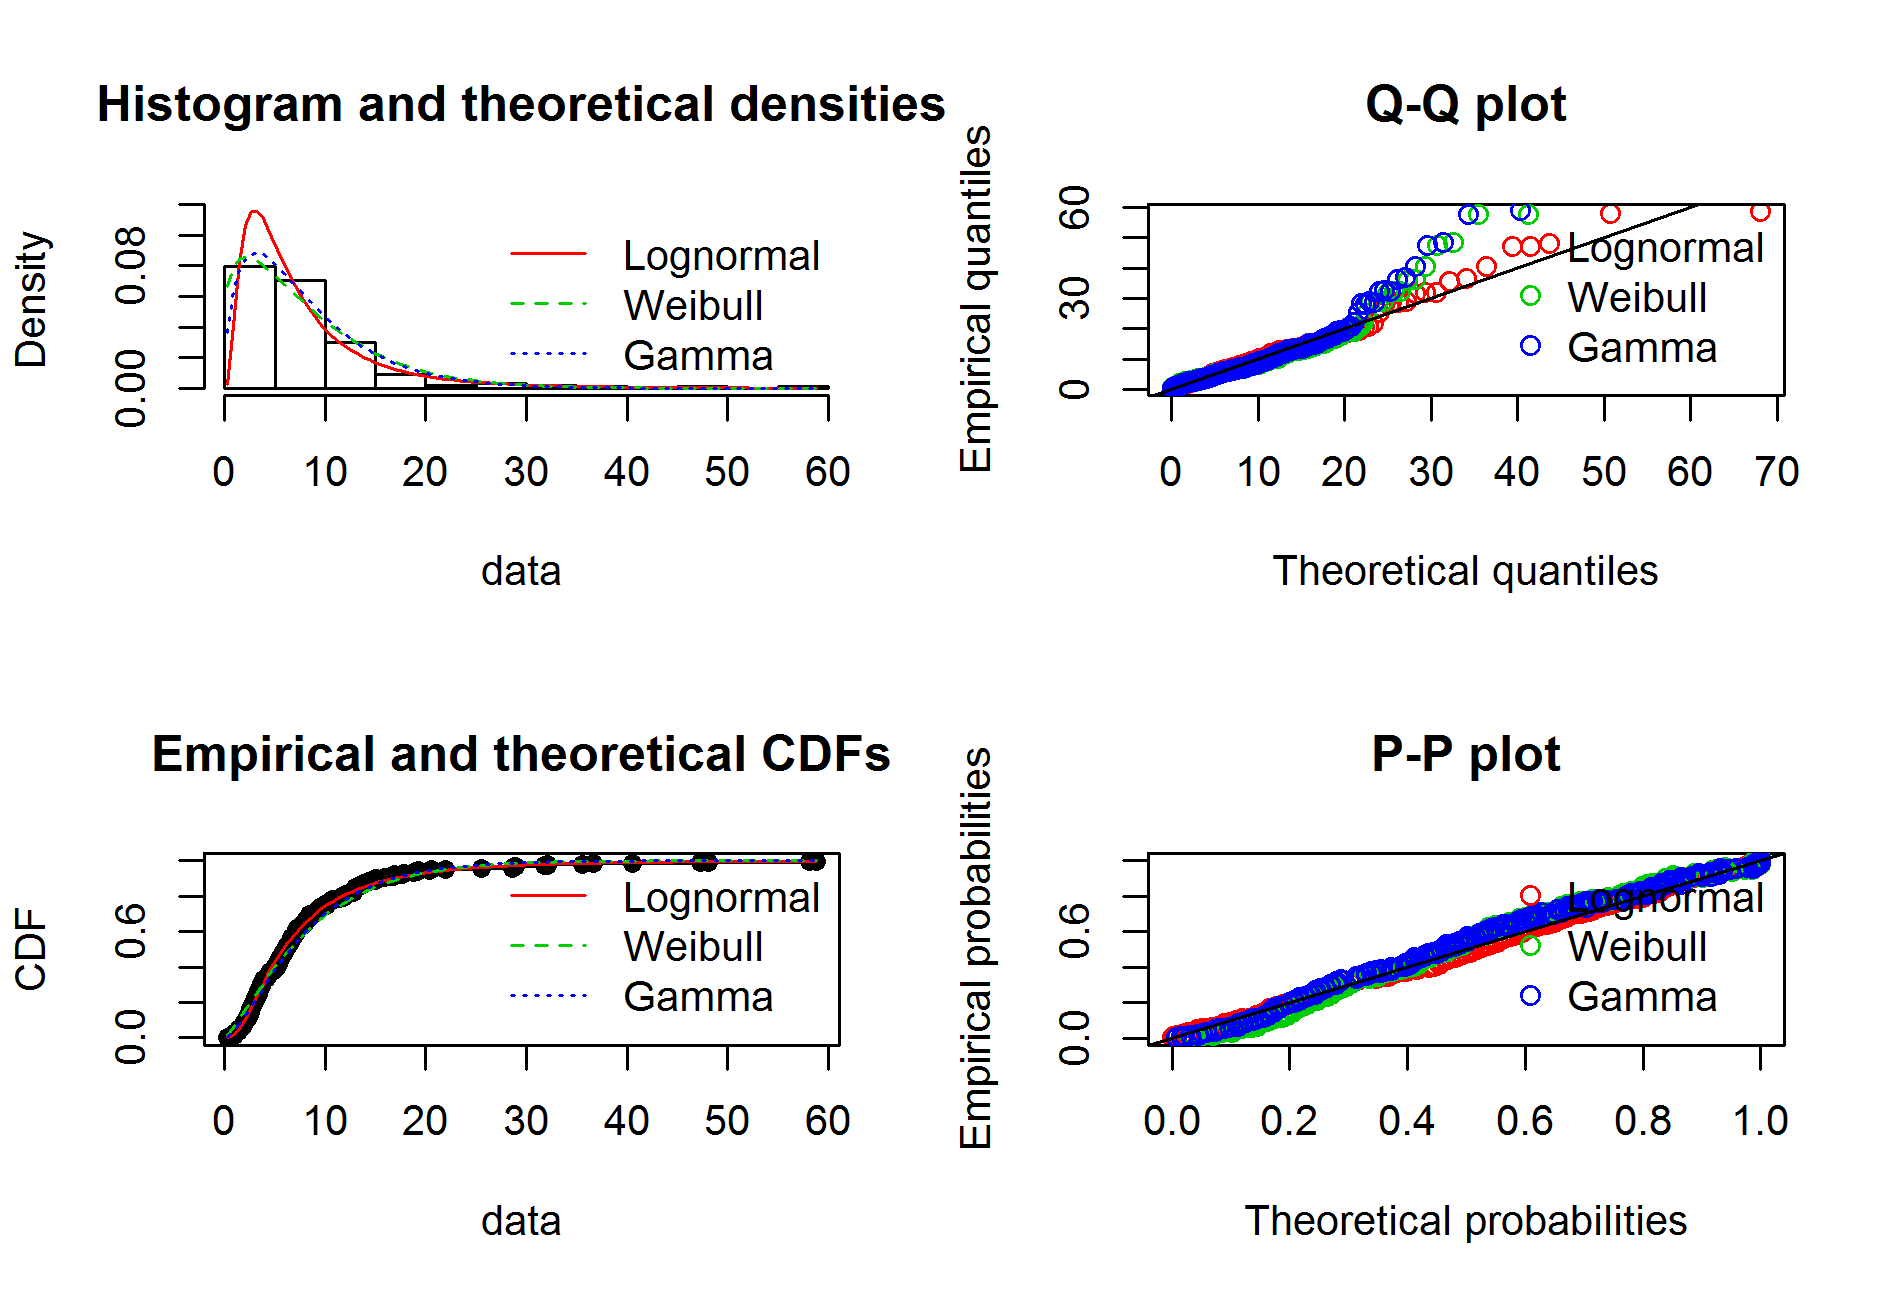
\includegraphics[width=.8\textwidth]{fig/gof_l3}
    \caption{Density plots of the fitted distributions to the histogram of the empirical distribution using the maximum expected lifespan data for trophic level 3, a CDF plot of both the empirical distribution and the fitted distributions (Gamma, Weibull, and Lognormal), Q-Q plots, and P-P plots. Plot created using R v.3.4.3 \cite{Rcite} fitdistrplus package v.$1.0-9$ \cite{fitdistrplus}. }
    \label{gof_l3}
\end{figure}

\begin{table}[H]
\centering
\caption{Goodness-of-fit criteria for maximum expected lifespan data at trophic level 4}
\begin{tabular}{r|c|c|c}
  \hline \small
 Goodness-of-fit criteria & Lognormal & Weibell & Gamma \\ 
   \hline
   Akaike's Information Criterion (AIC) & 1411.29 & 1426.64 & 1419.63 \\   
   Bayesian Information Criterion (BIC) & 1417.78 & 1433.14 & 1426.12 \\
   \hline
\end{tabular} 
\label{l4_aic}
\end{table}

\begin{figure}[H]
     \centering
       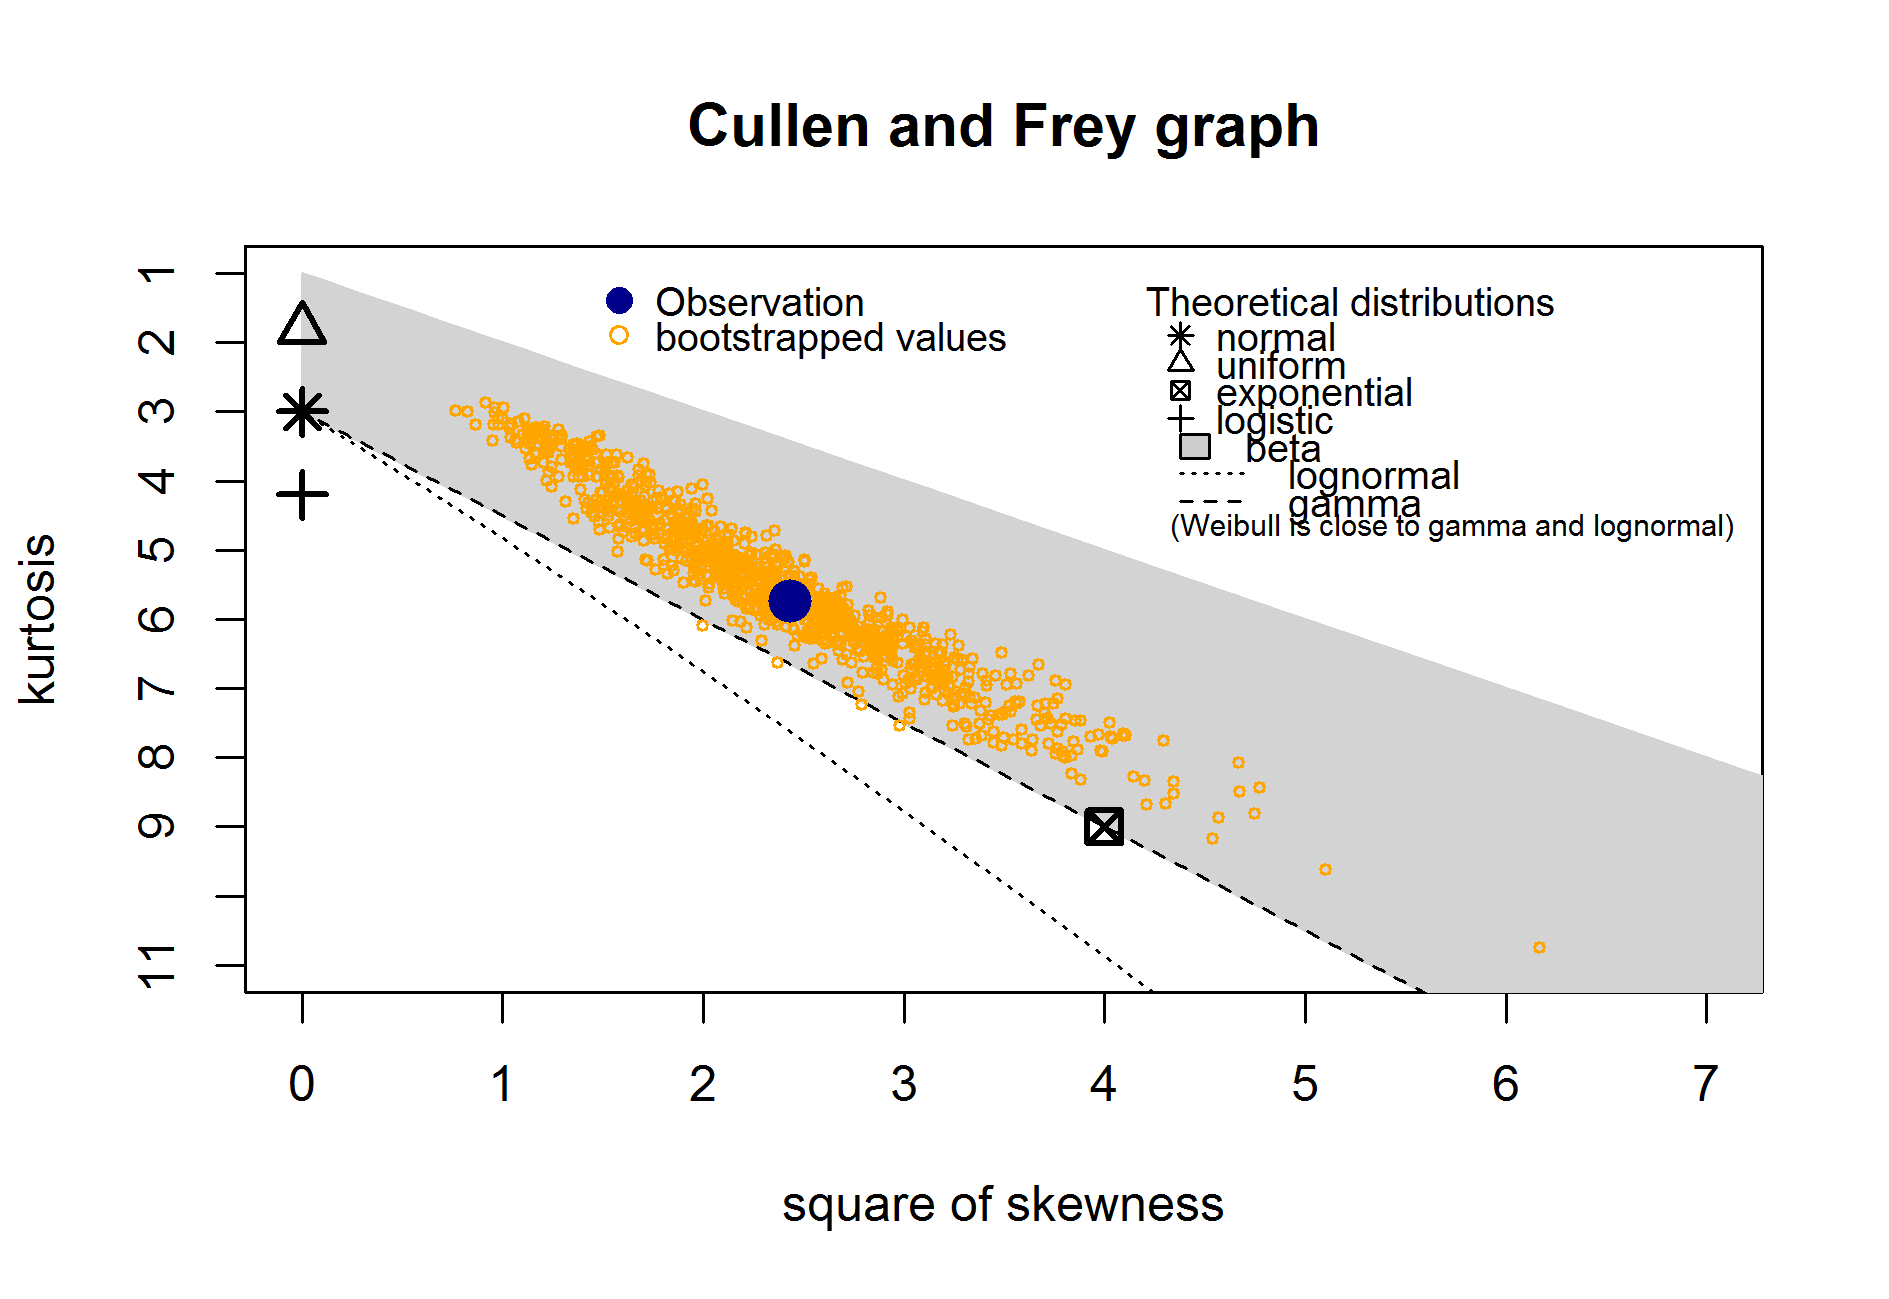
\includegraphics[width=.8\textwidth]{fig/cullen_frey_l4}
    \caption{Visualizes all potential continuous distributions against the maximum expected lifespan data for trophic level 4 and bootstrapped data. The figure shows it potentially follows a Gamma, Weibull, and Lognormal distribution. Plot created using R v.3.4.3 \cite{Rcite} fitdistrplus package v.$1.0-9$ \cite{fitdistrplus}. }
    \label{cf_l4}
\end{figure}

\begin{figure}[H]
     \centering
       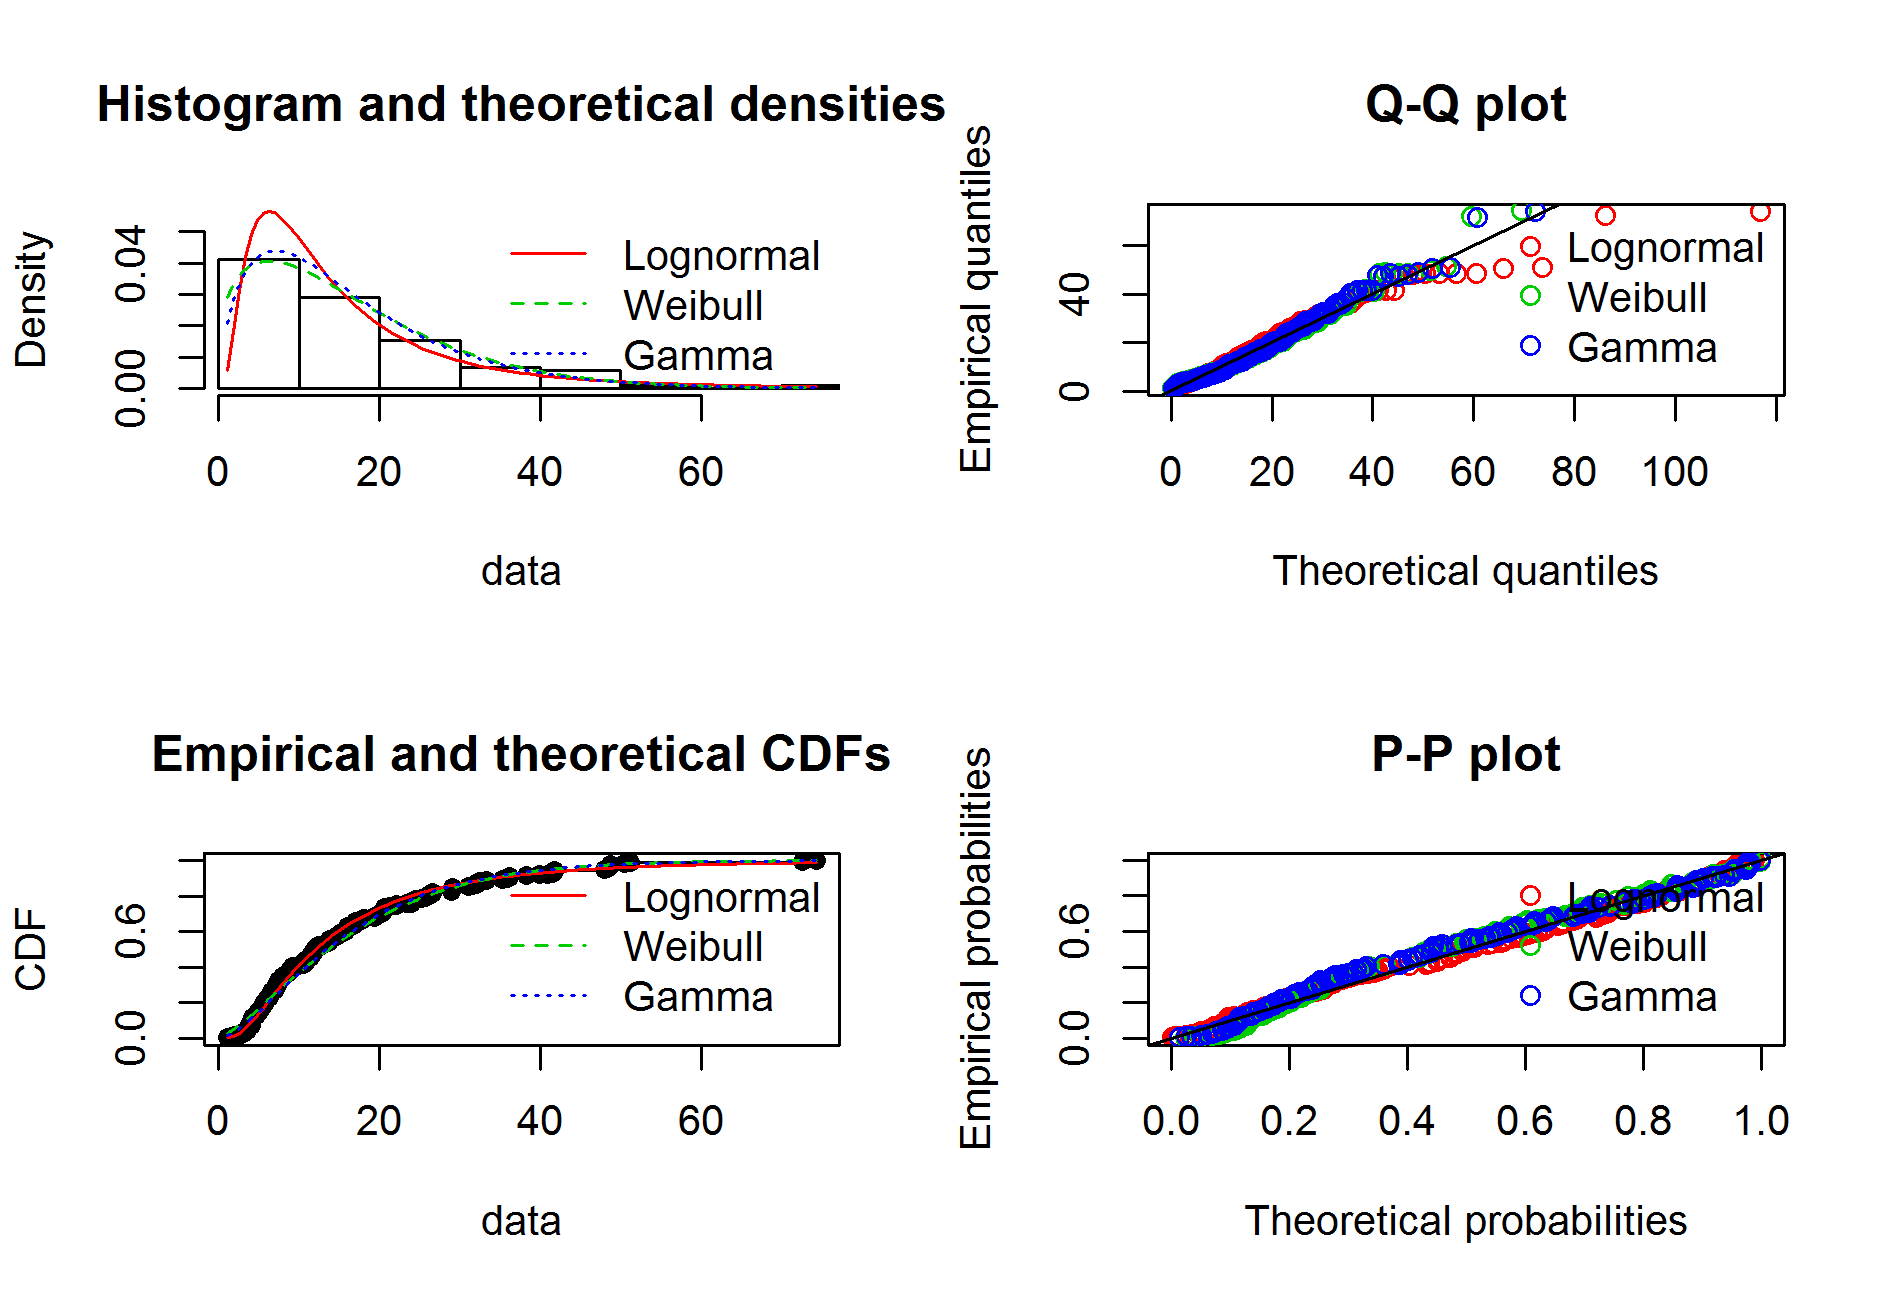
\includegraphics[width=.8\textwidth]{fig/gof_l4}
    \caption{Density plots of the fitted distributions to the histogram of the empirical distribution using the maximum expected lifespan data for trophic level 4, a CDF plot of both the empirical distribution and the fitted distributions (Gamma, Weibull, and Lognormal), Q-Q plots, and P-P plots. Plot created using R v.3.4.3 \cite{Rcite} fitdistrplus package v.$1.0-9$ \cite{fitdistrplus}. }
    \label{gof_l4}
\end{figure}


\section{Marginal Distributions}
When attempting to solve for the equations for the distributions of $\gamma_h$, we started off with the simplest stochastic scenario and progressed toward more complex cases.  
 
\subsection{Deriving Equations for Scenario NTl}
In Scenario NTl, both $\nu$ and $\tau_h$ are treated as fixed constants. We let $\lambda_h \sim Lognormal(\mu_{\lambda_h}, \sigma^2_{\lambda_h} )$ for $h \in \{2, 3, 4\}$ where $\mu_{\lambda_h}$ and $\sigma^2_{\lambda_h}$ are known constants. 

\vspace{5mm}

Beginning with the top layer in the hierarchical model (i.e., trophic level 2). We write  Eq. (1) from the main paper under Scenario NTl's assumptions where $c_{\nu9\tau_2}=\nu*9*\tau_2$.

\begin{equation*}
\gamma_2 = \nu * 9 * \tau_2 *\lambda_2  = c_{\nu9\tau_2} *\lambda_2 
\end{equation*}

From here, we are interested in determining the distribution of $c*\lambda_h$ assuming $c>0$. Since we let $\lambda_h \sim Lognormal(\mu_{\lambda_h}, \sigma^2_{\lambda_h})$, we can take the log to obtain $log(\lambda_h) \sim N(\mu_{\lambda_h}, \sigma^2_{\lambda_h})$. Therefore, $\gamma_h = c*\lambda_h$ can be transformed into $log(\gamma_h) = log(c*\lambda_h) = log(c) + log(\lambda_h)$. Using Jacobian transformations, we find that $log(\gamma_h) \sim N(\mu_{\lambda_h} + log(c), \sigma^2_{\lambda_h})$. Finally using the same logic as earlier, we conclude that $\gamma_h \sim Lognormal(\mu_{\lambda_h} + log(c), \sigma^2_{\lambda_h})$.

\vspace{5mm}

Therefore in Scenario NTl, trophic level biomass ($\gamma_h$) at each trophic level $h$ follows the following distributions:

\begin{equation}
\begin{split}
\gamma_2 & \sim Lognormal(\mu_{\lambda_2} + log(c'), \sigma^2_{\lambda_2}) \hspace{5mm} \text{where} \hspace{5mm} c' = \nu*9*\tau_2\\
\gamma_3 & \sim Lognormal(\mu_{\lambda_3} + log(c''), \sigma^2_{\lambda_3}) \hspace{5mm} \text{where} \hspace{5mm} c'' = \nu*9*\tau_2*\tau_3 \\
\gamma_4 & \sim Lognormal(\mu_{\lambda_4} + log(c'''), \sigma^2_{\lambda_4}) \hspace{5mm} \text{where} \hspace{5mm} c''' = \nu*9*\tau_2*\tau_3*\tau_4 \\
\end{split}
\end{equation}

\subsection{Deriving Equations for Scenario nTl}
In Scenario nTl, $\tau_h$ is treated as a fixed constant, and we treat $\nu \sim Lognormal(\mu_\nu, \sigma^2_\nu)$ and $\lambda_h \sim Lognormal(\mu_{\lambda_h}, \sigma^2_{\lambda_h} )$ for $h \in \{2, 3, 4\}$ where we assume the parameters for both $\nu$ and $\lambda_h$ are known constants. 

\vspace{5mm}

Beginning with the top layer in the hierarchical model (i.e., trophic level 2), we write Eq. (1) from the main paper under Scenario nTl's assumptions where $c_{9\tau_2}=9*\tau_2$.

\begin{equation*}
\gamma_2 = \nu * 9 * \tau_2 *\lambda_2  = \nu * c_{9\tau_2} *\lambda_2 
\end{equation*}

We want to determine the distribution when two random variables that follow distinct Lognormal distributions are multiplied together. If we let $\lambda_h' = ln(\lambda_h) \sim N(\mu_{\lambda_h}, \sigma^2_{\lambda_h})$ and $\nu' = ln(\nu) \sim N(\mu_\nu, \sigma^2_\nu)$, then using properties of Normal distributions we obtain that $Y' = \lambda_h' + \nu' \sim N(\mu_{\lambda_h} + \mu_\nu, \sigma^2_{\lambda_h} + \sigma^2_\nu)$. Remembering that $Y' = ln(\lambda_h) + ln(\nu)$, we can then raise it to the exponent fo find that $e^{Y'} = e^{ln(\lambda_h*\nu)} = \lambda_h*\nu$. We then find that $e^{Y'} \sim Lognormal(\mu_{\lambda_h} + \mu_\nu, \sigma^2_{\lambda_h} + \sigma^2_\nu)$. Using the theory outline in Scenario NTl pertaining constants ($c>0$) and Lognormal distributions, we conclude that $c*\lambda_h*\nu \sim Lognormal(\mu_{\lambda_h} + \mu_\nu + log(c),  \sigma^2_{\lambda_h} + \sigma^2_\nu)$.

\vspace{5mm}

Therefore in Scenario nTl, trophic level biomass ($\gamma_h$) at each trophic level $h$ follows the following distributions:

\begin{equation}
\begin{split}
\gamma_2 & \sim Lognormal \left( \mu_\nu + \mu_{\lambda_2} + log(c'), \sigma^2_\nu+\sigma^2_{\lambda_2} \right) \hspace{5mm} \text{where} \hspace{5mm} c' = 9*\tau_2 \\
\gamma_3 & \sim Lognormal \left( \mu_\nu + \mu_{\lambda_3} + log(c''), \sigma^2_\nu+\sigma^2_{\lambda_3} \right) \hspace{5mm} \text{where} \hspace{5mm} c'' = 9*\tau_2*\tau_3 \\
\gamma_4 & \sim Lognormal \left( \mu_\nu + \mu_{\lambda_4} + log(c'''), \sigma^2_\nu+\sigma^2_{\lambda_4} \right) \hspace{5mm} \text{where} \hspace{5mm} c''' = 9*\tau_2*\tau_3*\tau_4 \\
\end{split}
\end{equation}

\subsection{Attempting to Derive Equations for Scenario \textit{NtL}}
In Scenario \textit{NtL}, $\nu$ and $\lambda_h$ for $h \in \{2, 3, 4\}$ are treated as fixed constants. We let $\tau_h \sim Beta(\alpha_h, \beta_h)$ for $h \in \{2, 3, 4\}$ and assume $\alpha_h$ and $\beta_h$ are known constants for $\tau_h$.

\vspace{5mm}

Beginning with the top layer in the hierarchical model (i.e., trophic level 2), we write Eq. (1) from the main paper under Scenario \textit{NtL}'s assumptions where $c_{9\nu\lambda_2}=9*\nu\lambda_2$.

\begin{equation*}
\gamma_2 = \nu * 9 * \tau_2 *\lambda_2 = c_{\nu9\lambda_2}*\tau_2 
\end{equation*}

While we are interested in determining the distribution of $c*\tau_2$ assuming $c>0$,  no theorems exist that prove the beta distribution has the scaling property. In addition, at higher trophic levels we will be multiplying multiple independent Beta distributions. Therefore given the lack of extant research on the topic, we decided simulation was a reasonable option. 

\subsection{Attempting to Derive Equations for Scenario \textit{Ntl}}
In Scenario \textit{Ntl}, $\nu$ is treated as a fixed constant. We treat $\tau_h \sim Beta(\alpha_h, \beta_h)$ and $\lambda_h \sim Lognormal(\mu_{\lambda_h}, \sigma^2_{\lambda_h} )$ for $h \in \{2, 3, 4\}$. We assume $\mu_{\lambda_h}$ and $\sigma^2_{\lambda_h} $ are known constants for $\lambda_h$ and $\alpha_h$ and $\beta_h$ are known constants for $\tau_h$.

\vspace{5mm}

Beginning with the top layer in the hierarchical model (i.e., trophic level 2), we write Eq. (1) from the main paper under Scenario \textit{Ntl}'s assumptions where $c_{9\nu}=9*\nu$.

\begin{equation*}
\gamma_2 = \nu * 9 * \tau_2 *\lambda_2 = c_{\nu9}*\tau_2*\lambda_2 
\end{equation*}

While our goal was to determine the exact distribution of the product of two random variables that follow a Beta and a Lognormal distribution, extant research (e.g., \citealt{casella2002statistical, rohatgi2015introduction}) on the topic provides no clear path forward. The closest match were two papers on the distribution of the product of a Beta, Gamma, and mean zero Normal \cite{springer1970distribution, gaunt2018products}. 

\vspace{5mm}

\citealt{gaunt2018products} extends Stein's method to products of independent Beta, Gamma, generalized Gamma and mean zero Normal random variables. Gaunt defined a characteristic function outlined in Corollory 3.3 for the Product Beta, Product Gamma, and Product Normal where $W \sim N(0, \sigma^2)$. This Corollory derived from \citealt{gaunt2018products} state that a characteristic function can be found for the Product Beta, Product Gamma, and Product central Normal. However, we believe this proof is going to break down when moving from a symmetric to a non-symmetric distribution. 
Providing additional complexity, in Scenario \textit{Ntl} and the in the remaining scenarios, Lognormal distributions are used (as opposed to Normal distributions). 

\begin{figure}[H]
     \centering
       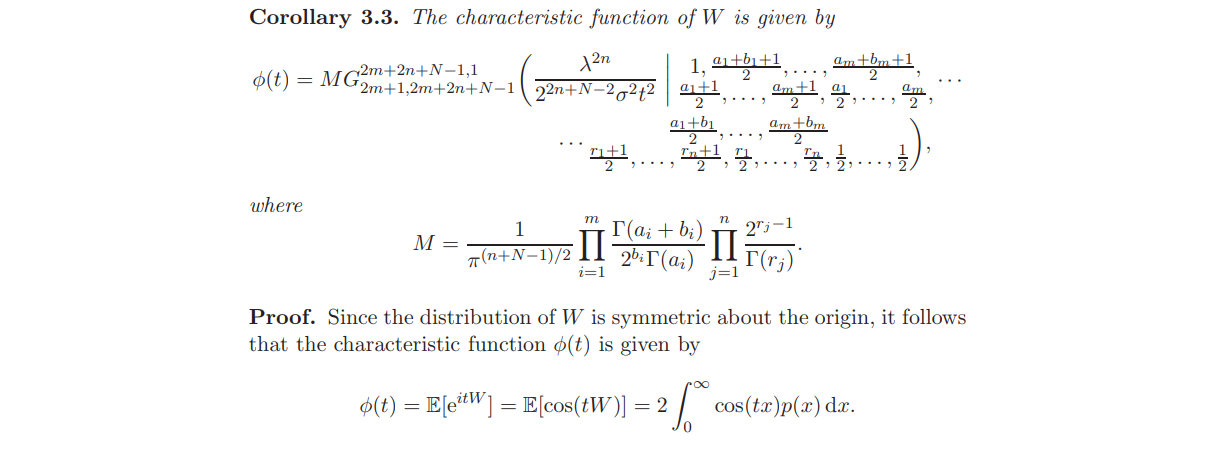
\includegraphics[width=1\textwidth]{fig/Stein}
\end{figure}

 
\section{Table of Distributions}

\begin{sidewaystable}
\caption{Table of Distributions}
\begin{tabular}{l|l|l}
  \hline \small
 Distribution & PDF & Mean \& Variances \\ 
   \hline
   Lognormal & \(\displaystyle f(\nu;\mu,\sigma^2) = \frac{1}{\sqrt{2\pi}\sigma \nu}exp\left( -\frac{(log(\nu)-\mu)^2}{2\sigma^2} \right) \hspace{2mm} \text{for} \hspace{2mm} \nu > 0 \) & \(\displaystyle E[\nu] = e^{\mu + \frac{\sigma^2}{2}} \) \\
      & &  \(\displaystyle Var[\nu] =  e^{2\mu + \sigma^2}(e^{\sigma^2} - 1) \) \\
   \hline
   Beta & \(\displaystyle f(\tau_{h};\alpha,\beta) = \frac{1}{B(\alpha, \beta)} \tau_{h}^{\alpha -1} (1-\tau_{h})^{\beta -1}  \hspace{2mm} 0 \leq \tau_{h} \leq 1   \) &  \(\displaystyle E[\tau_{h}] = \frac{\alpha}{\alpha + \beta} \) \\
	   & &  \(\displaystyle Var[{\tau_{h}}] = \frac{\alpha\beta}{(\alpha + \beta)^2(\alpha + \beta + 1)} \) \\
   \hline
\end{tabular} 
\label{distributions}
\end{sidewaystable}

\newpage

\section{R packages and versions}
To promote reproducibility, we include a list of all R packages and versions used in this analysis.

\begin{itemize}
\item astsa package v.1.8 \cite{astsa}
\item data.table package v.$1.10.4-3$  \cite{datatable}
\item ExtDist package v.$0.6-3$ \cite{extdist}
\item fitdistrplus package v.$1.0-9$ \cite{fitdistrplus}
\item forecast package v8.2 \cite{forecast1, forecast2} 
\item ggplot2 package v.2.2.1 \cite{ggplot}
\item gridExtra package v.2.3 \cite{gridextra}
\item gtable package v.0.2.0 \cite{gtable}
\item logspline package v.2.1.9 \cite{logspline}
\item R v.3.4.3 \cite{Rcite} 
\item reshape package v.0.8.7 \cite{reshape}
\end{itemize}


\chapter{Appendix for Chapter 4: Ecosystem knowledge in Bayesian surplus production models--what can it tell us?}{\label{appendix:c}}


\section{Data}
\subsection{SeaWiFS}
\subsubsection{Time Series Analysis}
In the trophic pyramid food web model, $\nu$ is the mean of the SeaWiFS time series (87339861.7 metric tons C/year) within the EEZ of the MHI found by fitting a seasonal autoregressive integrated moving average model (SARIMA model) to the SeaWiFS data using R v.3.4.3 \cite{Rcite} forecast package v8.2 and function auto.arima() \cite{forecast1, forecast2}. To find $\nu$, we used 8-day time series Sea-viewing Wide Field-of-view Sensor (SeaWiFS) chlorophyll \textit{a} data from 1997 to 2010 that was transformed using the \textit{Eppley-}Vertically Generalized Production Model (VGPM) to estimate net primary production (NPP) from chlorophyll \textit{a}. The \textit{Eppley-}VGPM estimates were used rather than the VGPM data since temperatures surrounding the main Hawaiian Islands (MHI) are above $20^{\circ}$C \cite{morel1991pigment, antoine1996oceanic, stock2017reconciling}. The SeaWiFS data were originally obtained from the Oregon State Ocean Productivity website (\url{http://www.science.oregonstate.edu/ocean.productivity/}). They use a gap filling algorithm to populate missing pixels due to cloud coverage; however if no good data is available, pixels remain empty. We segmented the SeaWiFS data using the exclusive economic zone (EEZ) boundaries of the MHI and assumed a closed system at equilibrium (Fig. \ref{A3:SeaWiFSmhi}). The data then were converted from 8 day averages in mg C / $m^2$ / day per 9 km x 9 km pixel into total metric tons of Carbon per year total across the entire MHI. Although from 1997 to 2010 SeaWiFS collected data every 8 days  per 9 km x 9 km pixel, the time series had gaps due to machine parts malfunctioning. Therefore, the updated data set used for our analysis contained observations only from 1998-2007. 

\begin{figure}[H]
     \centering
       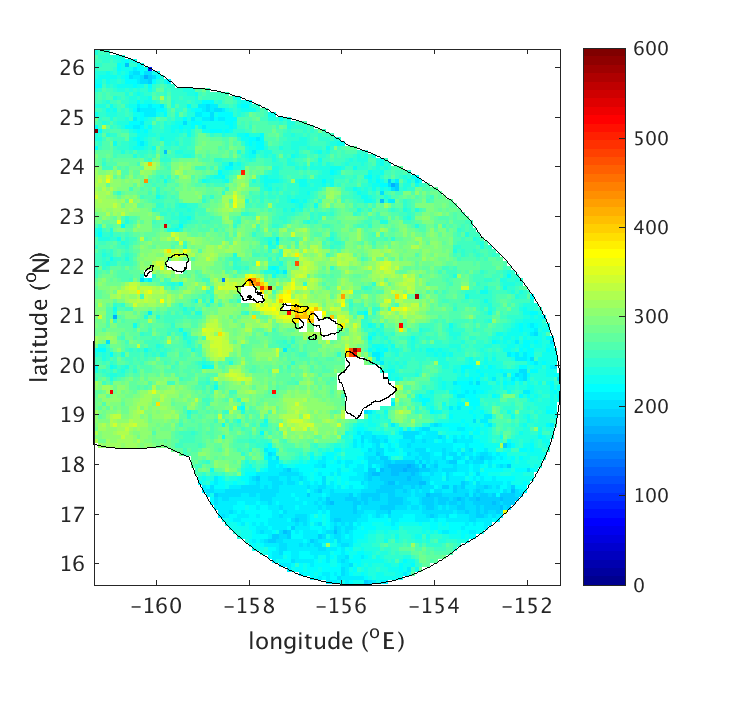
\includegraphics[width=.7\textwidth]{fig/SeaWiFSmhi}
    \caption{A single 8-day time frame of the SeaWiFS \textit{Eppley-}VGPM NPP data in January 1998 for the main Hawaiian Islands EEZ. The color scale shows the amount of estimated NPP in total gigatons of Carbon per year per pixel. The pixel size of the SeaWiFS data set is 9 by 9 km.}
    \label{A3:SeaWiFSmhi}
\end{figure}

Since the SeaWiFS data were collected over time, we started off by verifying that there was a violation of independence and then chose a usable time series model. The NPP data demonstrated a strong annual frequency, a smaller six month frequency, and were non-stationary in the trend and seasonality (See Fig. \ref{A3:SeaWiFSmhi_eda1}  and \ref{A3:SeaWiFSeda3}). This was not surprising since most biological data sets are seasonal and are influenced by the time of year. 

\begin{figure}[H]
     \centering
       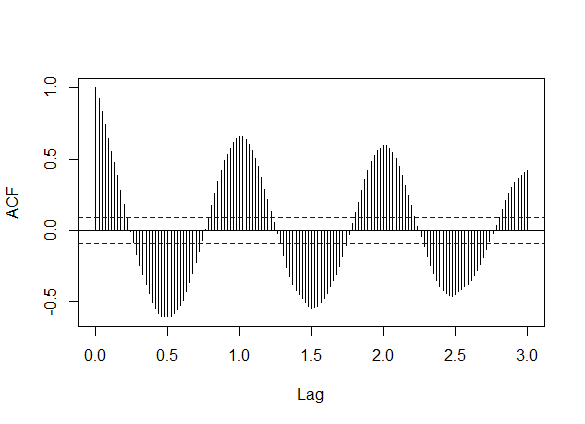
\includegraphics[width=.7\textwidth]{fig/seawifs_acf}
    \caption{ACF plot of SeaWiFS data. Plots created using R v.3.4.3 \cite{Rcite} forecast package v8.2 \cite{forecast1, forecast2}.}
    \label{A3:SeaWiFSeda1}
\end{figure}

\begin{figure}[H]
     \centering
       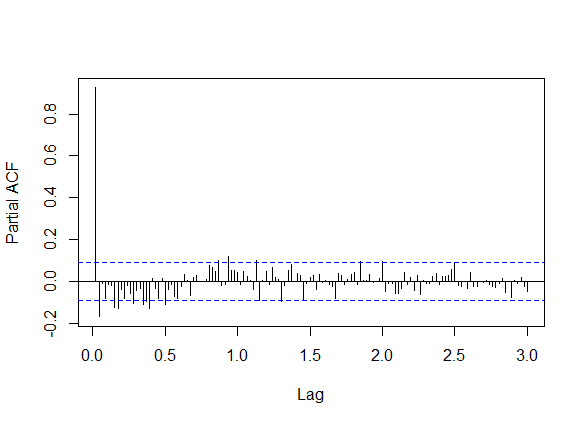
\includegraphics[width=.7\textwidth]{fig/seawifs_pacf}
    \caption{PACF plots of SeaWiFS data. Plots created using R v.3.4.3 \cite{Rcite} forecast package v8.2 \cite{forecast1, forecast2}.}
    \label{A3:SeaWiFSeda2}
\end{figure}

\begin{figure}[H]
     \centering
       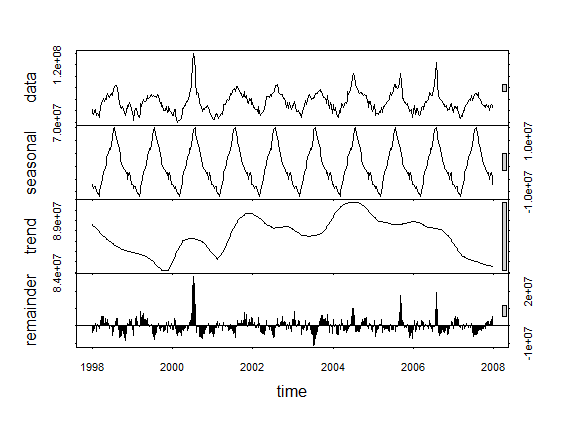
\includegraphics[width=.7\textwidth]{fig/seawifs_periodic}
    \caption{Exploratory time series plots of SeaWiFS data--seasonal and trend components. Plots created using R v.3.4.3 \cite{Rcite} forecast package v8.2 \cite{forecast1, forecast2}.}
    \label{A3:SeaWiFSeda3}
\end{figure}

We fitted a seasonal autoregressive integrated moving average model, or \\ SARIMA$(0,0,2)(0,0,2)_{46}$ to the pre-processed SeaWiFS NPP data (i.e., moving average order $q = 2$, seasonal moving average $Q = 2$, and seasonal component $s = 46$ (365 days/8-day time series = 46)).

\begin{equation} \label{sarima_a3}
X_t = \delta + (1 + \theta_1B + \theta_2B^2)(1 + \Theta_1B^{46} + \Theta_2B^{92})W_t
\end{equation}

In Eq. \ref{sarima_a3}, $X_t$ is the total NPP estimated across the MHI in 8-day time periods from 1998-2007 where $t \in$ \{1, 460\}, $\delta$ represents the mean of the time series, $\theta_1$ and $\theta_2$ are the moving average parameters, $\Theta_2$ and $\Theta_2$ are the seasonal moving average parameters, and $W_t \stackrel{iid}{\sim} N(0,\sigma_w^2)$. The backshift operator, B, is defined as $ BW_t  = W_{t-1}$, $B^2W_t  = W_{t-2}$, $B^{46}W_t  = W_{t-46}$, and $B^{92}W_t  = W_{t-92}$.  Our model, Eq. \ref{sarima_a3}, was chosen based on information criteria. Parameters were estimated using maximum likelihood estimation \cite{forecast1, forecast2}. The parameter estimates can be found in Table \ref{sarima_parameters_a3}. The estimate of parameter $\delta$ was used for the value of $\nu$ when it was treated as a fixed constant in the hierarchical food web model ($c_1$ in $f^1(\nu)$).

\begin{table}[H]
\centering
\caption{Seasonal ARIMA parameter estimates for Eq. \ref{sarima_a3} and their respective standard error calculated using R v.3.4.3 \cite{Rcite} forecast package v8.2 and function auto.arima() \cite{forecast1, forecast2} }
\begin{tabular}{r|c|c}
  \hline \small
 Parameters & Estimates & Standard error \\ 
   \hline
   $\delta$ & 87339861.7 & 696375.7 \\   
   $\theta_1$ & 0.9806 & 0.0413 \\
   $\theta_2$ & 0.4817 & 0.0359 \\
   $\Theta_1$ & 0.3379 & 0.0470 \\
   $\Theta_2$ & 0.3392 & 0.0449 \\
   $\sigma_w^2$ & 1.494306e+13 & \\
   \hline
\end{tabular} 
\label{sarima_parameters_a3}
\end{table}

\subsection{Transfer Efficiency}
We utilized data gathered from a literature review (i.e., Chapter 2: Tangled is the web we weave) on transfer efficiencies to fit an approximate distribution ($\tau_h$). The data includes articles that mentioned both food web and transfer efficiency and then selected from these studies those that included data whether model-based or empirical. We used all of the marine data (i.e., both model-based and empirical) to fit a distribution. The resulting distributional assumption was placed on transfer efficiencies ($\tau_h$) for all trophic levels $h \in \{2, 3, 4\}$. In order to determine an approximate distributions, we ran goodness-of-fit tests. We started off with skewness-kurtosis plots (Fig. \ref{cf_te_a3}) to initially decide which distributions to consider (i.e., Beta and Gamma) \cite{fitdistrplus}. Then we fitted individual distributions to the data using maximum likelihood estimation and compared density plots of the fitted distributions to the histogram of the empirical distribution, a cumulative distribution (CDF) plot of both the empirical distribution and the fitted distributions, Q-Q plots, and P-P plots (Fig. \ref{gof_te_a3}). Lastly, we used both AIC and BIC criterion to choose the most approximate distribution (Table \ref{te_aic_a3}). While the Gamma distribution was a reasonable choice, we preferred the Beta distribution, because the transfer efficiency is a percentage and the Beta distribution is defined within the range [0, 1]. Therefore, we concluded that the Beta distribution was the most appropriate approximate distribution. The probability distribution function (PDF) and equations for the mean and variance of a Beta distribution can be found in Table \ref{distributions_a3}.

\begin{table}[H]
\centering
\caption{Goodness-of-fit criteria for transfer efficiency data}
\begin{tabular}{r|c|c}
  \hline \small
 Goodness-of-fit criteria & Beta  & Gamma \\ 
   \hline
   Akaike's Information Criterion (AIC) & -354.94 & -369.97 \\   
   Bayesian Information Criterion (BIC) & -348.96 &  -363.99  \\
   \hline
\end{tabular} 
\label{te_aic_a3}
\end{table}

\begin{figure}[H]
     \centering
       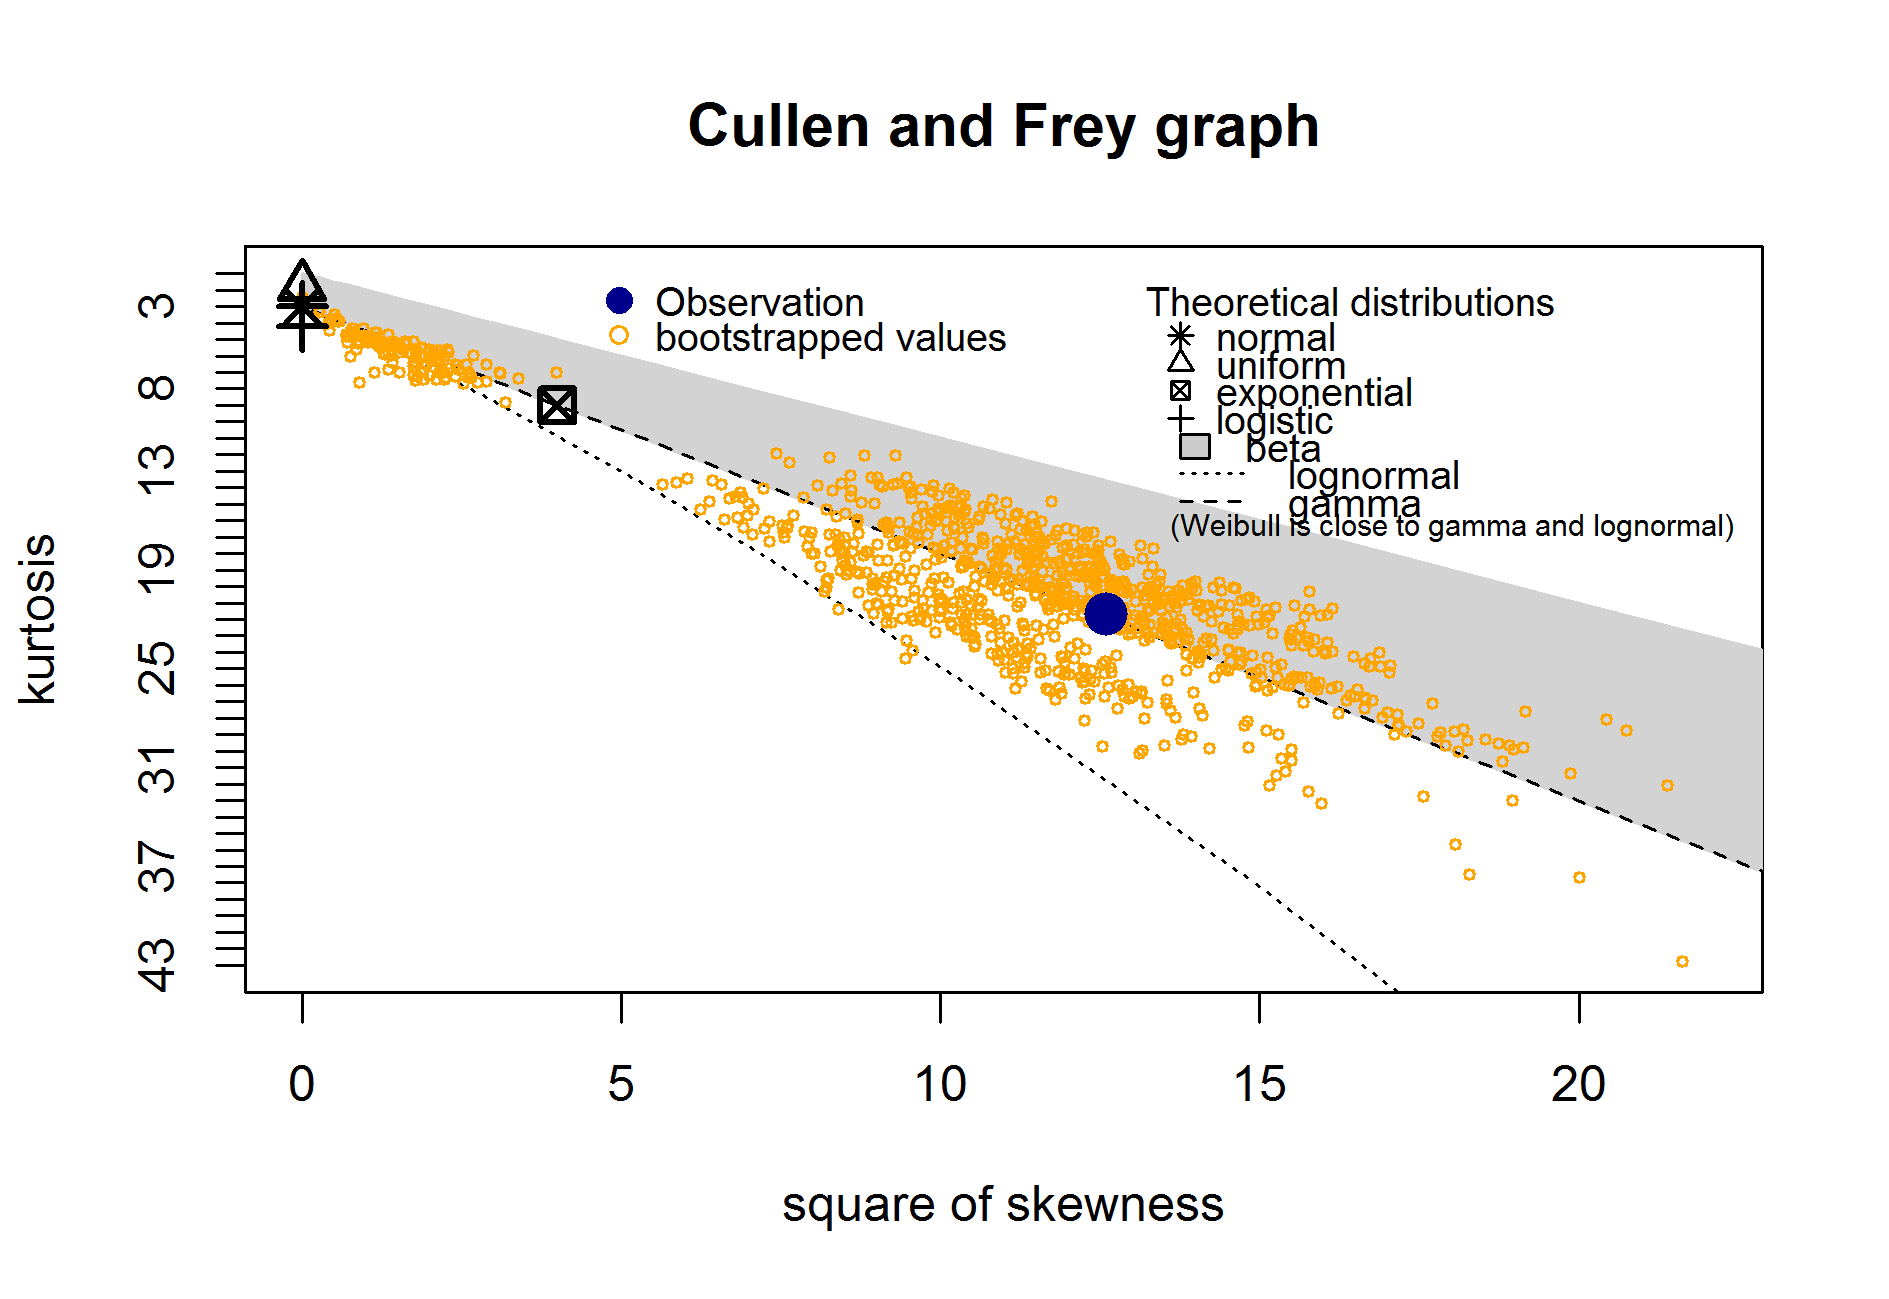
\includegraphics[width=.8\textwidth]{fig/cullen_frey_te}
    \caption{Visualizes all potential continuous distributions against the marine transfer data (Case 2) and bootstrapped data. The figure shows it potentially follows a Beta and Gamma distribution. Plot created using R v.3.4.3 \cite{Rcite} fitdistrplus package v.$1.0-9$ \cite{fitdistrplus}. }
    \label{cf_te_a3}
\end{figure}

\begin{figure}[H]
     \centering
       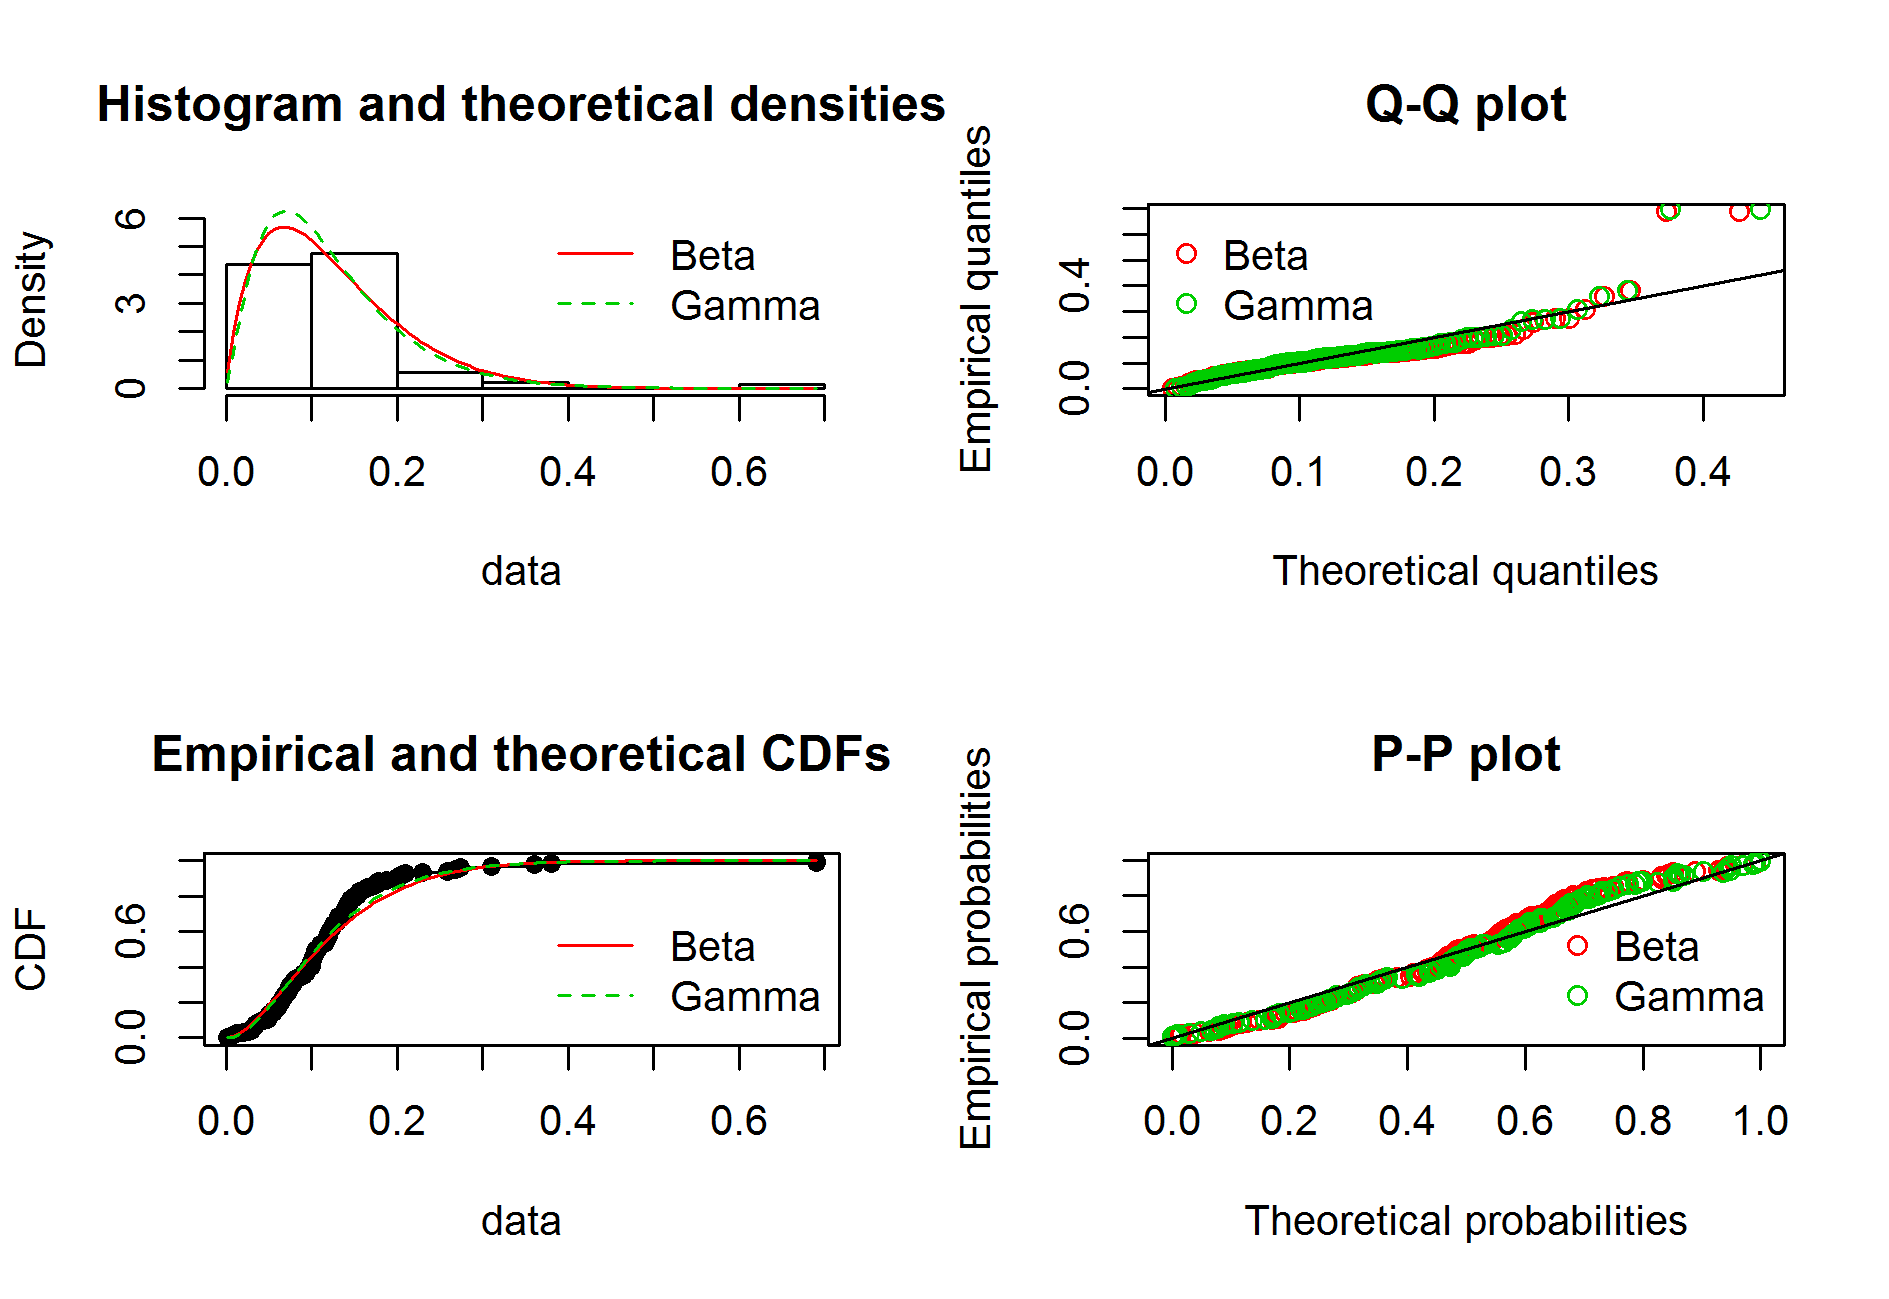
\includegraphics[width=.8\textwidth]{fig/gof_te}
    \caption{Density plots of the fitted distributions to the histogram of the empirical distribution using the marine transfer efficiency data (Case 2), a CDF plot of both the empirical distribution and the fitted distributions (Beta and Gamma), Q-Q plots, and P-P plots. Plot created using R v.3.4.3 \cite{Rcite} fitdistrplus package v.$1.0-9$ \cite{fitdistrplus}. }
    \label{gof_te_a3}
\end{figure}


\subsection{FishBase}
\subsubsection{Trophic Level}
Estimated trophic levels (rational numbers) were calculated from the FishBase database (\url{http://www.fishbase.org/}) for each species and truncated to cluster species into integer-valued trophic levels. Truncated trophic levels range in the MHI from $h=1,\dots,4$ with $h=1$ representing phytoplankton, $h=2$ primary consumers, $h=3$ secondary consumers, and $h=4$ tertiary consumers. If the rational number was greater than or equal to 4, then the organism was put into trophic level 4, if it was less than 4 and greater than or equal to 3 it was put into trophic level 3, and if it was less than 3 it was put into trophic level 2. The number of species found at each trophic level were not equal.


\subsubsection{Maximum Expected Lifespan}
The maximum expected lifespan $\lambda_4$ for species at trophic level $h = 4$ was treated as a random value. We ran goodness-of-fit tests to find an approximate distribution. We started off with a skewness-kurtosis plot (Fig. \ref{cf_l4_a3}) to initially decide which distributions to consider (i.e., Lognormal, Weibull, and Gamma) \cite{fitdistrplus}. Then we fitted individual distributions to the data using maximum likelihood estimation and compared density plots of the fitted distributions to the histogram of the empirical distribution, a cumulative distribution (CDF) plot of both the empirical distribution and the fitted distributions, Q-Q plots, and P-P plots (Fig. \ref{gof_l4_a3}). Lastly, we used AIC and BIC criterion to choose the most approximate distribution (Table \ref{l4_aic_a3}). We found for all trophic levels the most appropriate approximate distribution was a Lognormal distribution, where each trophic level has distinct values for $\mu$ and $\sigma^2$. 

\begin{table}[H]
\centering
\caption{Goodness-of-fit criteria for maximum expected lifespan data at trophic level 4}
\begin{tabular}{r|c|c|c}
  \hline \small
 Goodness-of-fit criteria & Lognormal & Weibell & Gamma \\ 
   \hline
   Akaike's Information Criterion (AIC) & 1411.29 & 1426.64 & 1419.63 \\   
   Bayesian Information Criterion (BIC) & 1417.78 & 1433.14 & 1426.12 \\
   \hline
\end{tabular} 
\label{l4_aic_a3}
\end{table}

\begin{figure}[H]
     \centering
       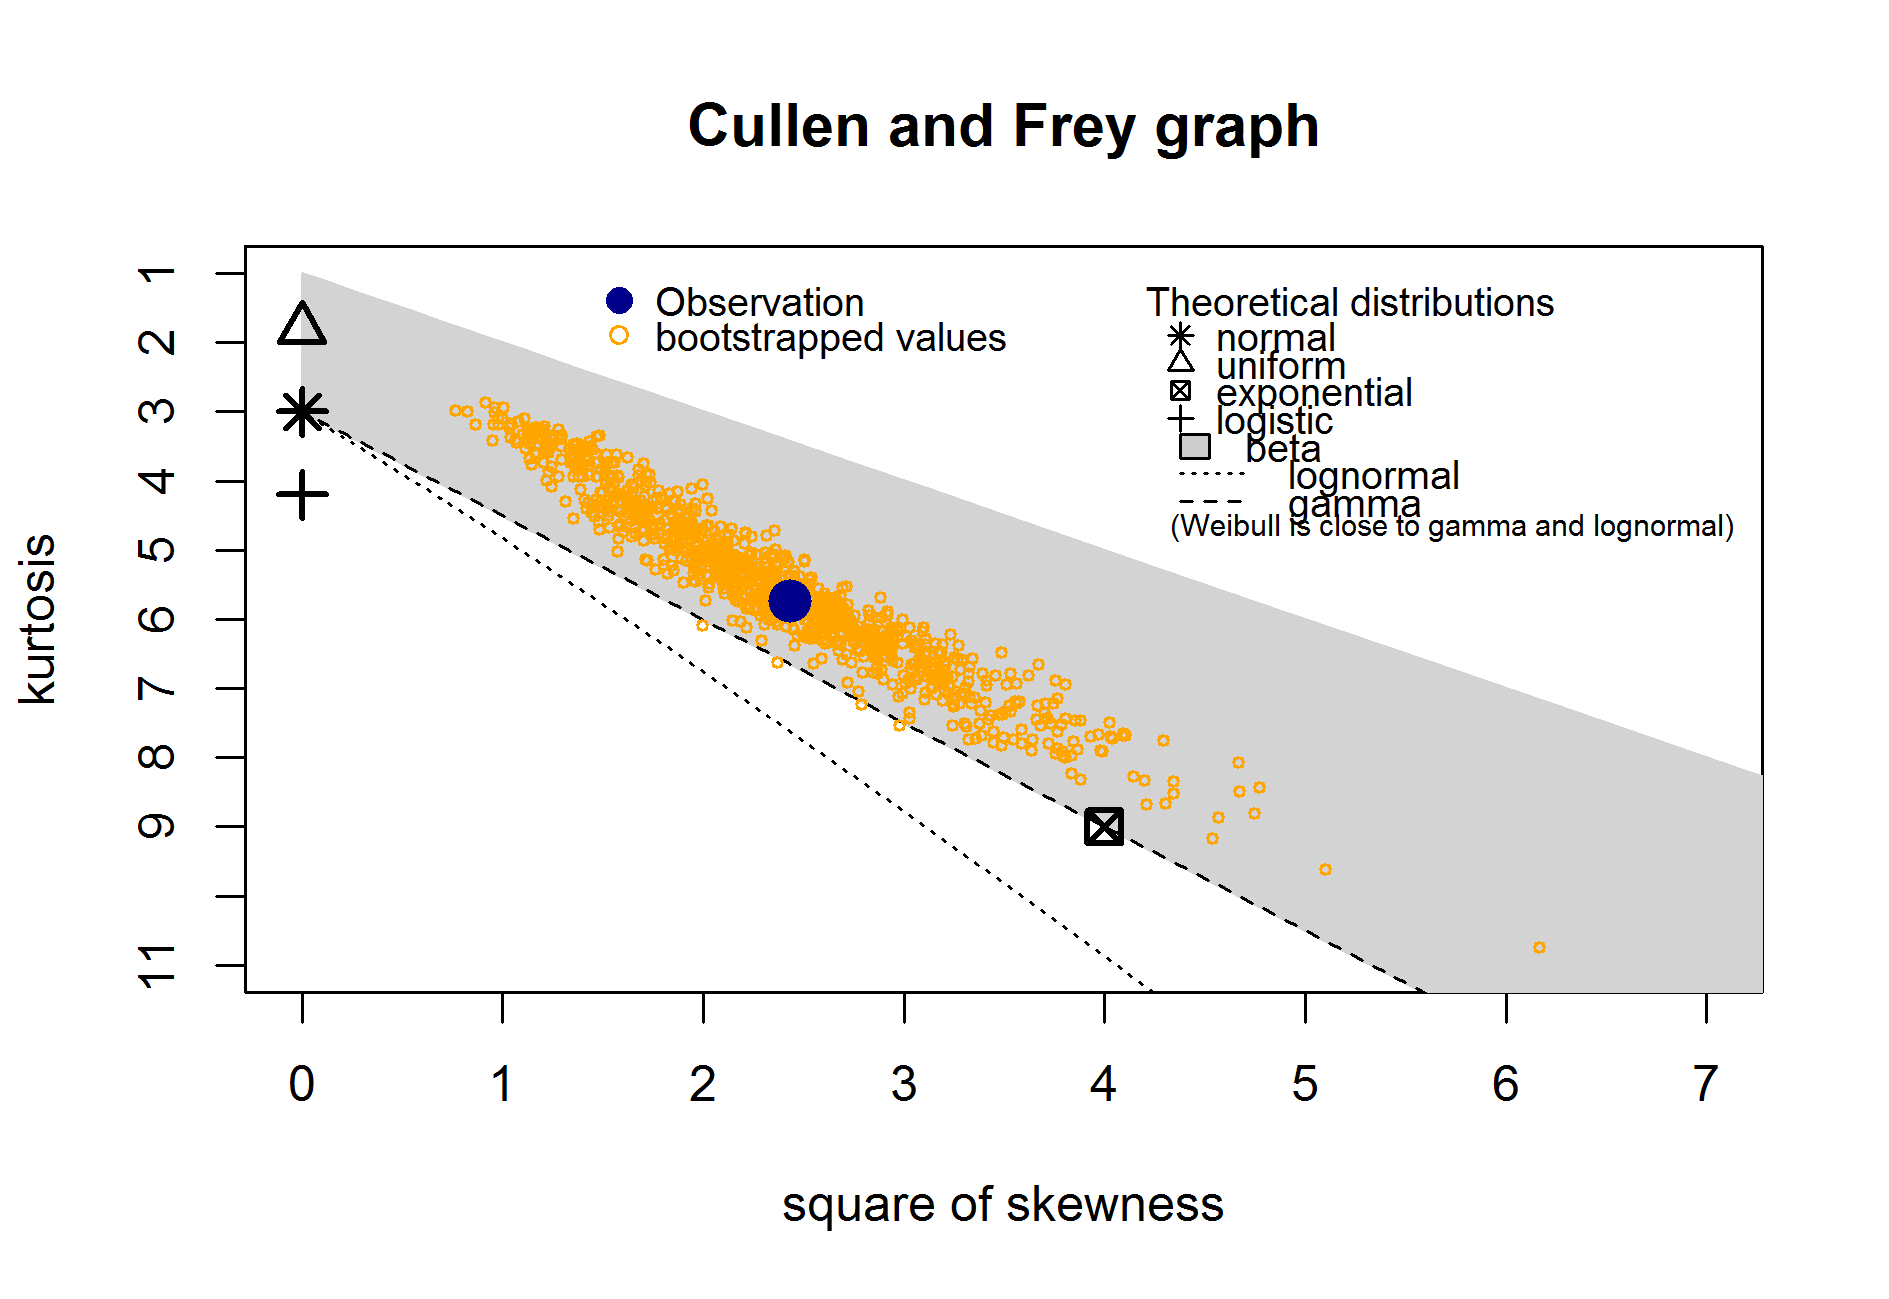
\includegraphics[width=.8\textwidth]{fig/cullen_frey_l4}
    \caption{Visualizes all potential continuous distributions against the maximum expected lifespan data for trophic level 4 and bootstrapped data. The figure shows it potentially follows a Gamma, Weibull, and Lognormal distribution. Plot created using R v.3.4.3 \cite{Rcite} fitdistrplus package v.$1.0-9$ \cite{fitdistrplus}. }
    \label{cf_l4_a3}
\end{figure}

\begin{figure}[H]
     \centering
       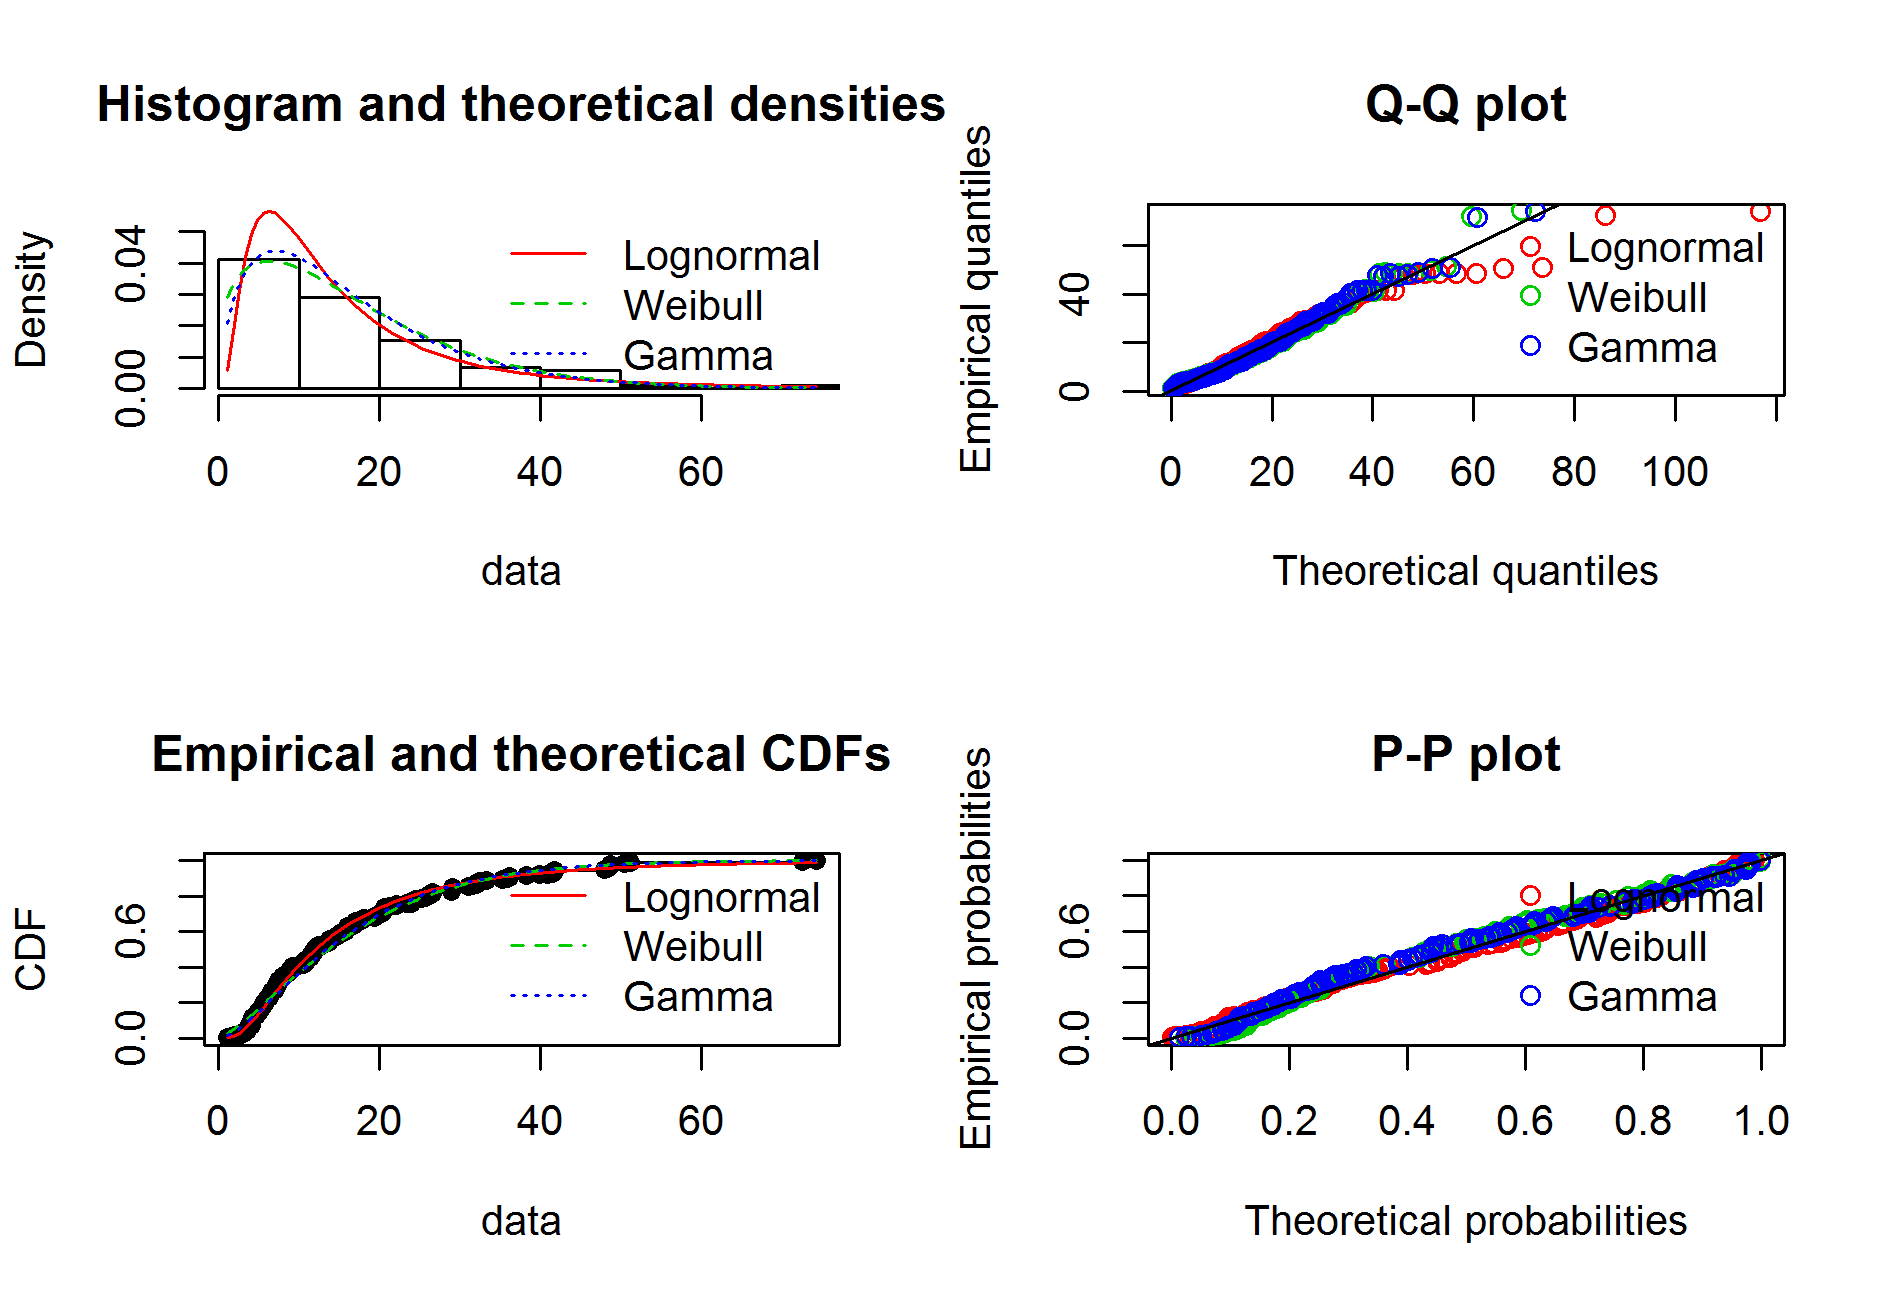
\includegraphics[width=.8\textwidth]{fig/gof_l4}
    \caption{Density plots of the fitted distributions to the histogram of the empirical distribution using the maximum expected lifespan data for trophic level 4, a CDF plot of both the empirical distribution and the fitted distributions (Gamma, Weibull, and Lognormal), Q-Q plots, and P-P plots. Plot created using R v.3.4.3 \cite{Rcite} fitdistrplus package v.$1.0-9$ \cite{fitdistrplus}. }
    \label{gof_l4_a3}
\end{figure}

\section{Table of Distributions}
\begin{sidewaystable}
\caption{Table of Distributions}
\begin{tabular}{l|l|l}
  \hline \small
 Distribution & PDF & Mean \& Variances \\ 
   \hline
   Lognormal & \(\displaystyle f(\nu;\mu,\sigma^2) = \frac{1}{\sqrt{2\pi}\sigma \nu}exp\left( -\frac{(log(\nu)-\mu)^2}{2\sigma^2} \right) \hspace{2mm} \text{for} \hspace{2mm} \nu > 0 \) & \(\displaystyle E[\nu] = e^{\mu + \frac{\sigma^2}{2}} \) \\
      & &  \(\displaystyle Var[\nu] =  e^{2\mu + \sigma^2}(e^{\sigma^2} - 1) \) \\
   \hline
   Beta & \(\displaystyle f(\tau_{h};\alpha,\beta) = \frac{1}{B(\alpha, \beta)} \tau_{h}^{\alpha -1} (1-\tau_{h})^{\beta -1}  \hspace{2mm} 0 \leq \tau_{h} \leq 1   \) &  \(\displaystyle E[\tau_{h}] = \frac{\alpha}{\alpha + \beta} \) \\
	   & &  \(\displaystyle Var[{\tau_{h}}] = \frac{\alpha\beta}{(\alpha + \beta)^2(\alpha + \beta + 1)} \) \\  	
   \hline
      Normal &  \(\displaystyle f(SS;\mu,\sigma^2) = \frac{1}{\sqrt{2\pi}\sigma }exp\left( -\frac{(SS-\mu)^2}{2\sigma^2} \right) \hspace{2mm} \text{for} \hspace{2mm} SS > 0 \) & \(\displaystyle E[SS] =\mu \) \\
      & &  \(\displaystyle Var[SS] =  \sigma^2 \) \\
\end{tabular} 
\label{distributions_a3}
\end{sidewaystable}

\newpage

\section{R packages and versions}
To promote reproducibility, we include a list of all R packages and versions used in this analysis.

\begin{itemize}
\item astsa package v.1.8 \cite{astsa}
\item data.table package v.$1.10.4-3$  \cite{datatable}
\item ExtDist package v.$0.6-3$ \cite{extdist}
\item fitdistrplus package v.$1.0-9$ \cite{fitdistrplus}
\item forecast package v8.2 \cite{forecast1, forecast2} 
\item ggplot2 package v.2.2.1 \cite{ggplot}
\item gridExtra package v.2.3 \cite{gridextra}
\item gtable package v.0.2.0 \cite{gtable}
\item MCMCpack package v.$1.4-2$ \cite{mcmcpack}
\item logspline package v.2.1.9 \cite{logspline}
\item R v.3.4.3 \cite{Rcite} 
\item reshape package v.0.8.7 \cite{reshape}
\item xtable package v.$1.8-2$ \cite{xtable}
\end{itemize}





\end{mainmatter}

%----- Bibliography ----------------
\ssp
\newcommand{\newblock}{}
\bibliographystyle{apalike}
\bibliography{dissertation}

\end{document} 
